% ##############################################
% Start: Template Preamble
% ##############################################
%
\listfiles
% Documentclass definition
\input{01_Preamble/documentclass.tex}

% Loading additional packages from the KOMA-Script family
\input{01_Preamble/KOMA-Script-Packages.tex}

% Page layout definition
\input{01_Preamble/PageLayout.tex}

% Standard packages
% Input encoding is 'latin1' (Latin 1 - also known as ISO-8859-1)
% CTAN: http://www.ctan.org/pkg/inputenc
%
% A newer package is available - you may look into:
% \usepackage[x-iso-8859-1]{inputenc}
% CTAN: http://www.ctan.org/pkg/inputenx
\usepackage[latin1]{inputenc}%OK

% Font Encoding is 'T1' -- important for special characters such as Umlaute � or � and special characters like � (enje)
% CTAN: http://www.ctan.org/pkg/fontenc
\usepackage[T1]{fontenc, url}%OK
\usepackage[bitstream-charter]{mathdesign}

% Language support for 'english' (alternative 'ngerman' or 'french' for example)
% CTAN: http://www.ctan.org/pkg/babel
\usepackage[english]{babel} %OK
\usepackage[babel]{csquotes}
\usepackage{hyphenat}
\hyphenation{tem-pe-ra-tu-re}

% Doing calculations with LaTeX units -- needed for the vertical line in the footer
% CTAN: http://www.ctan.org/pkg/calc
\usepackage{calc}%OK

% Extended graphics support
% There is also a package named 'graphics' - watch out!
% CTAN: http://www.ctan.org/pkg/graphicx
\usepackage{graphicx}%OK

% Extendes support for floating objects (tables, figures), adds the [H] placing option (\begin{figure}[H]) which palces it "Here" (without any doubt).
% CTAN: http://www.ctan.org/pkg/float
\usepackage{float}

% Support for captions, subcaptions and subfigures
\usepackage{subcaption}
\usepackage{caption}
\captionsetup{justification=centering}

% Extended color support
% I use the command \definecolor for example.
% Option 'Table': Load the colortbl package, in order to use the tools for coloring rows, columns, and cells within tables.
% CTAN: http://www.ctan.org/pkg/xcolor
\usepackage[table]{xcolor}

% Nice tables
% CTAN: http://www.ctan.org/pkg/booktabs
\usepackage{booktabs}%OK

% Better support for ragged left and right. Provides the commands \RaggedRight and \RaggedLeft.
% Standard LaTeX commands are \raggedright and \raggedleft
% http://www.ctan.org/pkg/ragged2e
\usepackage{ragged2e}

% Create function plots directly in LaTeX
% CTAN: http://www.ctan.org/pkg/pgfplots
\usepackage{pgfplots}
\pgfplotsset{compat=1.11}

%Create appendix
\usepackage[toc,page]{appendix}

% Create table of contents for each chapter
% CTAN: http://www.ctan.org/pkg/minitoc
\usepackage{minitoc}
\setcounter{minitocdepth}{2}

% Create nice bibliography
% CTAN: http://www.ctan.org/pkg/biblatex
\usepackage[backend=biber, bibstyle=authoryear, citestyle=authoryear-comp, sortcites, url=true, doi=true, dashed=false, indexing, backref=true, sorting=nyt]{biblatex}%refsection=chapter,
\AtEveryCite{\color{myColorMainA}}
\usepackage{guit}
\urlstyle{sf}

%Create list of abbreviations
\usepackage[acronym]{glossaries}

%Create analytical index
\usepackage{makeidx}
\DeclareIndexFieldFormat{indextitle}{}{}{}

%for schemes and pictures
\usepackage{tikz}
\usetikzlibrary{calc}

%Auxiliary packages for styling
\usepackage[protrusion=true,expansion=true]{microtype}

\usepackage[color=yellow,linecolor=white,textsize=footnotesize]{todonotes} % 

\usepackage{nicefrac}

\usepackage[binary-units=true]{siunitx}
\sisetup{per-mode = symbol-or-fraction}
\sisetup{detect-family = true}

%for nice tables
\usepackage{array}
\newcolumntype{P}[1]{>{\centering\arraybackslash}p{#1}}
\newcolumntype{M}[1]{>{\centering\arraybackslash}m{#1}}

\usepackage{longtable}
\usepackage{rotating}
\usepackage{tabularx}

\newcolumntype{s}{>{\hsize=.5\hsize}X}

\newcommand{\heading}[1]{\centering{\textbf{#1}}}

% ####-Important-####
%
% Definition of the two main colors
% -----------------------
% The corresponding xcolor package ist loaded in the file
% 01_Preamble/StandardPackages.tex
%
% ####-Important-####
\definecolor[named]{myColorMainA}{RGB}{0,26,153}
\definecolor[named]{myColorMainB}{RGB}{174,49,54}
% Customization of:
% - Floating Objects (Caption)
% - Table of Contents (TOC)
% - List of Figures
% - List of Tables
% - Headings (like chapter, section, etc.)
\input{01_Preamble/Floating-AND-TOC-AND-ListOf-AND-Headings.tex}

% Customization of the header, footer and teh margin note
\input{01_Preamble/HeaderFooterMarginnote.tex}

% Optimize paragraphs (avoid overfull... warnings)
\input{01_Preamble/ParagraphOptimization.tex}

% PDF related packages
\input{01_Preamble/PDF-Related.tex}

% PDF related packages
% Package to create test text -- just for demonstration purposes
% The command \blindtext produces a test text -- good for testing the layout
% CTAN: http://www.ctan.org/pkg/blindtext
\usepackage[]{blindtext}
% The custom command \myMarginnote is defined in the file: 
% 01_Preamble/HeaderFooterMarginnote.tex
\renewcommand{\blindmarkup}[1]{\myMarginnote{#1}}

% Custom commands for style
\DeclareMathVersion{mathchartertext}
\SetSymbolFont{letters}{mathchartertext}{OML}{mdbch}{m}{n}
\newcommand{\charmu}{\mathversion{mathchartertext}$\mu$\mathversion{normal}}

%\newcommand\ReferencesList{}
%\newcommand\AddtoRefsList[1]{\xdef\ReferencesList{\ReferencesList,#1}}
%\AtEveryCitekey{\AddtoRefsList{\thefield{entrykey}}}

%\makeatletter
%\patchcmd{\blx@addbackref@i}{\c@refsection}{\c@savedrefsection}{}{}

%\newcounter{savedrefsection}
%\newcommand\saverefsection{%
%  \protected@write\@mainaux{}{\string\setcounter{savedrefsection}{\the\c@refsection}}%
%}
%\makeatother

\newcounter{oldtocdepth}

\newcommand{\hidefromtoc}{%
  \setcounter{oldtocdepth}{\value{tocdepth}}%
  \addtocontents{toc}{\protect\setcounter{tocdepth}{-10}}%
}

\newcommand{\unhidefromtoc}{%
  \addtocontents{toc}{\protect\setcounter{tocdepth}{\value{oldtocdepth}}}%
}

%Title page Packages
\usepackage{amsmath}
\usepackage{tikz}
\usepackage{epigraph}
\usepackage{lipsum}
\usepackage{addfont}
\addfont{OT1}{cmpica}{\pica}

\renewcommand\epigraphflush{flushright}
\renewcommand\epigraphsize{\normalsize}
\setlength\epigraphwidth{0.7\textwidth}

%\definecolor{titlepagecolor}{cmyk}{1,.60,0,.40}
\definecolor{titlepagecolor}{RGB}{0,26,153}


%\DeclareFixedFont{\titlefont}{T1}{ppl}{b}{it}{0.5in}
\DeclareFixedFont{\titlefont}{T1}{qag}{b}{it}{0.43in}


\makeatletter
\def\printuniv{%
    {\large \@author}}
\makeatother
\author{%
    Universit\'{e} Claude Bernard Lyon 1\\
    Physics departement\\
    Doctoral school ED52: Physics and Astrophysics\vspace{20pt} \\
    }

% The following code is borrowed from: https://tex.stackexchange.com/a/86310/10898

\newcommand\titlepagedecoration{%
\begin{tikzpicture}[remember picture,overlay,shorten >= -10pt]

\coordinate (aux1) at ([yshift=-15pt]current page.north east);
\coordinate (aux2) at ([yshift=-380pt]current page.north east);
\coordinate (aux3) at ([xshift=-3.8cm]current page.north east);
\coordinate (aux4) at ([yshift=-150pt]current page.north east);

\begin{scope}[titlepagecolor,line width=12pt,rounded corners=12pt]
\draw
  (aux1) -- coordinate (a)
  ++(225:4) --
  ++(-45:5.1) coordinate (b);
\draw[shorten <= -10pt]
  (aux3) --
  (a) --
  (aux1);
\draw[opacity=0.3,titlepagecolor,shorten <= -10pt]
  (b) --
  ++(225:2.2) --
  ++(-45:2.2);
\end{scope}
%\draw[titlepagecolor,line width=8pt,rounded corners=8pt,shorten <= -10pt]
%  (aux4) --
 % ++(225:0.8) --
  %++(-45:0.8);
\begin{scope}[titlepagecolor!70,line width=6pt,rounded corners=8pt]
\draw[shorten <= -10pt]
  (aux2) --
  ++(225:3) coordinate[pos=0.45] (c) --
  ++(-45:3.1);
\draw
  (aux2) --
  (c) --
  ++(135:2.5) --
  ++(45:2.5) --
  ++(-45:2.5) coordinate[pos=0.3] (d);
\draw
  (d) -- +(45:1);
\end{scope}
\end{tikzpicture}%
}


%
% #######################
% End: Template Preamble
% #######################

%%Adding bibliography files
%\addbibresource{05_Bibliography/Biblio_13.bib}
\addbibresource{05_Bibliography/thesis.bib}

% ##############################################
% Start: Document
% ##############################################
%
% ------------------------------------------------------------------


\newglossaryentry{henry}{name={\ensuremath{\alpha_\mathrm{H}}},description={Solubility (a.k.a. Partitioning coefficient) \ensuremath{c_\mathrm{water} = \alpha_\mathrm{H} \cdot c_\mathrm{air}} } }



% *****  ACRONYMS  ************

%%%%%%%%%%%%%%%%%% Institutions - collaborations - groups %%%%%%%%%%%%%%%%%%%%%%%%%
\newacronym{ipnl}{IPNL}{Institut de Physique Nucl\'{e}aire de Lyon}
\newacronym{lpsc}{LPSC}{Laboratoire de Physique Subatomique et Corpuscolaire}
\newacronym{lpc}{LPC}{Laboratoire de Physique de Clermont}
\newacronym{creatis}{CREATIS}{Centre de Recherche en Acquisition et Traitement de l'Image pour la Sant\'{e}}
\newacronym{cppm}{CPPM}{Centre de Physique des Particules de Marseille}
\newacronym{clarys}{CLaRyS}{Contr\^{o}le en Ligne de l’hadronth\'{e}rapie par Rayonnements Secondaires - Online monitoring of ion beam therapy through secondary particles}
\newacronym{ganil}{GANIL}{Grand Accelerateur National d'Ions Lourds}
\newacronym{hit}{HIT}{Heidelberg Ion Therapy Center}
\newacronym{ipno}{IPNO}{Institut de Physique Nucl\'{e}aire d'Orsay}
\newacronym{lal}{LAL}{Laboratoire de l'Acc\'{e}l\'{e}rateur Lin\'{e}aire}
\newacronym{irfu}{IRFU}{Institut de Recherche sur les lois Fondamentales de l'Univers}
\newacronym{micrhau}{MICRHAU}{Micro-\'{e}lectronique RH\^{o}ne AUvergne}

%%%%%%%%% Materials %%%%%%%%%%%%%%%%
\newacronym{bgo}{BGO}{Bismuth Germanium Oxide - Bi$\mathrm{_{12}}$GeO$\mathrm{_{20}}$}
\newacronym{cdte}{CdTe}{Cadmium Telluride}
\newacronym{pmma}{PMMA}{Poly Methyl Metacrylate}
\newacronym{naitl}{NaI(Tl)}{Sodium Iodide doped with Thallium}
\newacronym{lyso}{LYSO}{Lutetium-Yttrium OxyorthoSilicate - Lu$\mathrm{_{2(1-x)}}$Y$\mathrm{_{2x}}$SiO$\mathrm{_{5}}$}
\newacronym{baf2}{BaF$_2$}{Barium Fluoride}


%%%%%%%%%%%% Detectors and utils %%%%%%%%%%%%%%%%%%%%%%
\newacronym{tof}{TOF}{Time-Of-Flight}
\newacronym{fwhm}{FWHM}{Full Width at Half Maximum}
\newacronym{enc}{ENC}{Equivalent Noise Charge}
\newacronym{dssd}{DSSD}{Double-sided Silicon Strip Detector}
\newacronym{hegp}{HEGP}{High Energy General Purpose}
\newacronym{pm}{PM}{Photo-Multiplier}
\newacronym{fe}{FE}{Front-End}
\newacronym{asic}{ASIC}{Application-Specific Integrated Circuit}
\newacronym{led}{LED}{Light Emitting Diode}
\newacronym{adc}{ADC}{Analog-to-Digital Converter}
\newacronym{tdc}{TDC}{Time-to-Digital Converter}
\newacronym{nim}{NIM}{Nuclear Instrumentation Module}
\newacronym{utca}{\charmu-TCA}{Micro Advanced Telecommunications Computing architecture}
\newacronym{rms}{RMS}{Root Mean Square}
\newacronym{csa}{CSA}{Charge Sensitive Amplifier}
\newacronym{shs}{SHS}{Slow Shaper}
\newacronym{fpga}{FPGA}{Field Programmable Gate Array}
\newacronym{lvds}{LVDS}{Low-Voltage Differential Signaling}
\newacronym{cr-rc}{CR-RC}{Capacitor Resistor - Resistor Capacitor}
\newacronym{dll}{DLL}{Delay Locked Loop}

%%%%%%%%%%%% Code and software utils %%%%%%%%%%%%%%%%%%%%%
\newacronym{geant4}{GEANT4}{GEometry And Tracking 4}
\newacronym{lm-mlem}{LM-MLEM}{List Mode-Maximum Likelihood Expectation Maximization}
\newacronym{megalib}{MEGAlib}{Medium-Energy Gamma-ray Astronomy library}
\newacronym{gate}{GATE}{GEANT4 Application for Tomographic Emission}


%%%%%%%%%%%%% Medical physics %%%%%%%%%%%%%%%%%%%
\newacronym{pet}{PET}{Positron Emission Tomography}
\newacronym{spect}{SPECT}{Single Photon Emission Computed Tomography}
\makeglossaries

\makeindex

\begin{document}

\dominitoc
%\dominilof
%\dominilot

\pagenumbering{gobble}
%Thesis cover page
%\frontmatter
\hidefromtoc

%%%%%%%%%%%%%%%%
% modèle de page de garde pour une thèse de l'Université de Lyon (version de mars 2016)
% Attention ! Encodage UTF8 ! Sinon adapter en conséquence...
%%%%%%%%%%%%%%%%

\documentclass[11pt,a4paper]{book}

\usepackage[utf8]{inputenc}
\usepackage[T1]{fontenc}
\usepackage{graphicx}
\usepackage[frenchb]{babel}
\usepackage[inner=2.5cm,outer=2.5cm, top=2.5cm, bottom=2.5cm]{geometry}

\begin{document}

\setlength{\parindent}{0pt}
\thispagestyle{empty}


\begin{center}
\includegraphics[height=3cm]{logo} %le fichier "logo" doit être dans le même dossier que le fichier tex
\end{center}


\fontsize{11pt}{13pt}\selectfont
N\textsuperscript{o} d'ordre NNT : xxx

\vspace{1cm}

\begin{center}
\fontsize{14pt}{16pt}\selectfont
\textbf{\uppercase{Thèse de doctorat de l'université de Lyon}}\\
\fontsize{12pt}{14pt}\selectfont
opérée au sein de\\
\textbf{l'Université Claude Bernard Lyon 1}

\vspace{0.5cm}

\textbf{École Doctorale ED52\\% rectifier le numéro d'accréditation
Physique et Astrophysique de Lyon}% nom complet de l'école doctorale

\vspace{0.5cm}

\textbf{Spécialité de doctorat :\\
Discipline : Physique m\'{e}dicale} % éventuellement


\vspace{1.5cm}

Soutenue publiquement/à huis clos le jj/12/2018, par :\\
\fontsize{14pt}{16pt}\selectfont
\textbf{Mattia Fontana}

\vspace{1.5cm} % adapter à la longueur du titre

\rule[20pt]{\textwidth}{0.5pt}

\fontsize{25pt}{28pt}\selectfont
\textbf{Gamma camera development for ion beam therapy monitoring and nuclear medicine applications}

\rule{\textwidth}{0.5pt}

\vspace{2cm} % adapter à la longueur du titre
\end{center}

\fontsize{12pt}{14pt}\selectfont
Devant le jury composé de :
\bigskip

\fontsize{11pt}{13pt}\selectfont

Nom Prénom, grade/qualité, établissement/entreprise \hfill Président(e) % mention "président" à ne préciser qu'après la soutenance

\bigskip

Nom Prénom, grade/qualité, établissement/entreprise \hfill  Rapporteur(e)

Nom Prénom, grade/qualité, établissement/entreprise \hfill Rapporteur(e)

Nom Prénom, grade/qualité, établissement/entreprise \hfill Examinateur/trice

Nom Prénom, grade/qualité, établissement/entreprise \hfill Examinateur/trice

\bigskip

Testa \'{E}tienne, grade/qualité, établissement/entreprise \hfill Directeur de thèse

L\'{e}tang Jean Michel, grade/qualité, établissement/entreprise \hfill Co-directeur de thèse % le cas échéant

Dauvergne Denis, grade/qualité, établissement/entreprise \hfill Invité % le cas échéant

\newpage

%\fontsize{12pt}{14pt}\selectfont   % si le document général n'est pas en police 11pt, décommenter et préciser la taille utilisée
% Suite du manuscrit
\end{document}

% Empty page after title page
\cleardoublepage

%Change geometry after cover page

\newgeometry{% siehe geometry.pdf (Figure 1)
	bottom=30mm,
	showframe=false, % For debugging: try true and see the layout frames
	%showframe=true, % For debugging: try true and see the layout frames
	margin=30mm,
	marginparsep=3mm,
	marginparwidth=20mm
}

% Title page
%% Title page using \maketitle (a more flexible alternative is the titlepage environment)
\title{PHD Thesis}
\subtitle{Tests and characterization of gamma
cameras for ion beam therapy monitoring and nuclear
medicine application.}
\author{Mattia Fontana}
\date{03.12.2018}
\maketitle
\begin{titlepage}

\noindent
\textcolor{myColorMainA}{\titlefont Tests and characterization \newline of gamma
cameras for \newline medical applications}\par
\epigraph{PhD Candidate}%
{\textsc{Mattia Fontana}}

\epigraph{Thesis directors}%
{\textsc{\'{E}tienne Testa} and \textsc{Jean Michel L\'{e}tang}}
\null\vfill
\vspace*{1cm}
\noindent
\hfill
\begin{minipage}{0.35\linewidth}
    \begin{flushright}
        \printuniv 
        Defended on December the \nth{14} 2018
    \end{flushright}
\end{minipage}
%
\begin{minipage}{0.02\linewidth}
    \rule{1pt}{125pt}
\end{minipage}
\titlepagedecoration
\end{titlepage}



% Empty page after title page
\cleardoublepage

% Activate header and footer defined in the file:
% 01_Preamble/HeaderFooterMarginnote.tex
\pagestyle{scrheadings}

% Activate roman numbering 
\pagenumbering{roman}

% Start with page 1 (I)
\setcounter{page}{1}

% Prologue
%\input{02_Chapters/Prologue.tex}

% Abstract
% Chapter without numbering but with appearance in the Table of Contents
% \addchap is a command from KOMA-Script
%\addchap{Abstract}
\chapter*{Abstract}


Ion beam therapy is a promising technique in cancer treatment because of the ion defined range and favorable dose delivery features. Strict and precise treatment planning and monitoring are now key points for the method developments and full exploitation. In particular, with the aim of optimizing the ion treatment effectiveness, the ion range monitoring is mandatory: different solutions have been explored, but an online treatment check is still a challenge. 
The ion beam treatment monitoring is mainly performed by means of secondary charged or neutral particles. In this context, the detection of the prompt-gammas (PG) emitted during treatments has proven its potential in the ion range control in real time. Since the first evidence of the existing correlation between the emitted gamma profile fall-off and the Bragg peak position, several groups are involved in research activities in order to develop and optimize instruments and methods with the aim of improving this monitoring technique.  Among the others, collimated and Compton cameras are being studied and optimized for this application. The same detectors can also be employed in nuclear medicine for the detection of the radioactive elements decay products.      



A collaboration of 5 institutions in France is involved in the parallel development of two composite detectors for ion beam monitoring and nuclear medicine application, and this thesis is carried out within this collaboration with the detectors clinical trial as final aim.



The project started a few years ago and is now at the final stage. The two cameras have been designed according to simulation studies, and the different components are now under tests.
The collimated camera is composed by a multi-slit tungsten mechanical collimator, set in front of an absorber composed of 96 BGO blocks, for a total size of 380x380x30 mm$^{3}$; each block presents a streaked surface with a 8x8 pixel matrix and the signal is read-out by 4 photomultipliers. A $\sim$3 ns time resolution can be achieved for the prompt gamma detection. The same absorber is part of the Compton camera, in addition to a scatterer section composed by 7 Double-Sided Silicon Detectors 96x96x2 mm$^{3}$ each.
With the collimated camera, the parallel emitted photons are selected by the collimator and a mono-dimensional emission profile can be reconstructed. The Compton camera has a more efficient detection technique, being absent a mechanical collimation system, and could potentially lead to 3D information thanks to the reconstruction of the Compton cone. 
In both cases an additional detector component is needed to temporally tag the incoming beam ions and help rejecting the relevant background (mostly due to neutrons) which strongly affects the prompt gamma yield. A scintillating fiber tagging hodoscope is then under development: it is composed by 128x2 perpendicular scintillating fibers, read-out from both sides by 8 64-channel silicon photomultipliers by Hamamatsu. 
The thesis work consists in the critical evaluation, characterization and tuning of the different components, together with the associated electronics, and of the complete detectors on beam. In parallel, simulation studies can improve the detection technique and optimize the detector structure, as well as pave the way for further applications.    

\cleardoublepage

% Table of Contents and Lost of Figures/Tables
\input{02_Content/Lists/TOC-AND-ListOf.tex}

\cleardoublepage

% Activate arabic numbering 
\pagenumbering{arabic}

% Start with page 1
\setcounter{page}{1}

\unhidefromtoc

% Prologue
\input{02_Content/Abstract_preThesis/Prologue.tex}

% Introduction
\chapter{Context}\label{chap::1}

\vfill

\minitoc

\newpage


\glsresetall

\section{Ion beam therapy}

\subsection{Physics}

\subsection{Advantages and drawbacks}

\subsection{Range verification}

\subsection{Secondary radiation techniques}

\subsubsection{Positron Emission Tomography}
PET techniques are based on the detection of the two back-to-back 511~keV photons produced by the annihilation of positrons (created by the emitter fragments of nuclear reactions) with patient electrons, resulting in a delayed radiation which should be detected with time coincidences, allowing for an intrinsic background reduction. Nevertheless, the monitoring with positron emitters secondary signal must deal with a limited count rate compared to medical imaging PET, with the lifetime of emitters providing a delayed information that implies the signal integration over a whole treatment fraction (not a single spot or group of spots), with physiological washout effects depending on to the emitters lifetime.

Even if the only available and functional range monitoring system in a clinical center is based on this technique~\parencite{Enghardt2004}, several clinical experience with commercial or adapted PET system already shown intrinsic limitations mainly connected to the ring geometry (not directly applicable to the treatment monitoring due to the presence of the beam) or in general to geometrical constraints limiting the field of view and the resulting system global efficiency and spatial accuracy (the limited detection angle generates artifacts in the final image)~\parencite{Parodi2016}. The research is ongoing and new results are expected for the next years thanks to the introductions of new systems with adapted geometries, to the improvements in acquisition and reconstruction techniques and to the clinical introduction of time-of-flight systems, intrinsically able to improve the detector spatial resolution via interaction time information, and depth-of-interaction reconstruction, which will allow for a more precise spatial reconstruction for reduced angular artifacts effects.

\subsection{Prompt-gammas: physics and features}



\subsection{State of the art of range verification and prompt-gamma techniques}


\section{Nuclear medicine}

\subsection{PET and SPECT}

\subsection{Comparison, advantages and drawbacks}

\subsection{State of the art of SPECT}


\clearpage
%\printbibliography[heading=subbibintoc]


% Main Part
\chapter{Gamma detection in medicine}\label{chap::2}

\vfill

\minitoc

\newpage

\glsresetall

As described in chapter~\ref{chap::1}, the detection of gamma photons plays a role of utmost importance in medical physics, for what concerns both the monitoring of ion beam therapy treatments and the nuclear medicine examination techniques. 

Ion beam therapy is rapidly emerging as a valuable cancer treatment technique and a superior alternative to photon radiotherapy for specific clinical indications. The narrow dose peak at the end of the ion range allows for targeted delivery of high dose to the tumor while sparing healthy surrounding tissues. However, since such a treatment technique is highly sensitive to dose prediction and delivery uncertainties, online range monitoring solutions are necessary. Over- and under-shooting effects potentially lead to severe damages to healthy tissues and/or treatment inefficiency, and thus have to be controlled in real-time. The research effort in this field mainly focuses on the non-invasive detection of primary by-products of beam-tissue nuclear interactions: photons from electron-positron annihilation and prompt gammas are most extensively studied for this purpose. 

In nuclear medicine diagnostics, radioactive tracers are injected in the patient body and the gamma rays, products of the tracer isotope decay, exiting the patient are detected to retrieve physiological and anatomical information. Positrons are emitted by $\beta^+$-decaying isotopes, and the two back-to-back photons generated by their annihilation with patient electrons are detected in time coincidences in \gls{pet} techniques. On the other hand, \gls{spect} exploits single photons emitted by $\gamma$-decaying isotopes with collimated detectors.

The research work presented in this thesis focus on the development of gamma cameras for the detection of prompt gamma rays to tackle the challenge of real-time range monitoring during particle therapy treatments. In addition, the developed prototype design has been tested for application in nuclear medicine \gls{spect}-like examinations. 
In this chapter, after a brief introduction about the photon interaction channels in matter, the main techniques based on gamma detection developed in the two mentioned fields are described, and the state-of-the-art of gamma detectors employed for these two purposes is sketched.

\section{Photon interactions in matter}\label{chap2::subsec::PhotonInteractions}

In penetrating an absorbing medium, photons may experience various interactions with the atoms of the medium, involving either the nuclei or the orbital electrons. The interactions with nuclei may be direct photon-nucleus collisions or interactions between the photon and the electrostatic field of the nucleus (pair production). On the other hand, the photon-orbital electron interactions can involve either loosely bound electrons (binding energy $E_B$ small in comparison with the photon energy $h\nu$ - $E_B \ll h\nu$) or tightly bound electrons (binding energy comparable to, or slightly smaller than the photon energy - $E_B  \lesssim h\nu$). 
All these processes are characterized by a partial or complete energy transfer of the gamma-ray photon, and two different outcomes are possible:
\begin{itemize}
\item Photon disappears (i.e. is completely absorbed) and its energy is transferred to light charged particles (electron and positrons);
\item Photon is scattered and two results are possible:
	\begin{itemize}
		\item the resulting photon has the same energy as the incident photon and no light charged particle is released in the interaction;
		\item the resulting scattered photon has a lower energy than the incident photon and the energy excess is transferred to a light charged particle (electron).
	\end{itemize}
\end{itemize}

We focus here on the interaction channels which play an important role in radiation measurements: 
\begin{itemize}
\item photoelectric absorption;
\item Compton scattering;
\item pair production.
\end{itemize}

In case the photon interacts with an absorber \myMarginnote{Photoelectric absorption} atom and completely disappears by transferring all its energy to the target, the interaction mechanism is called photoelectric absorption. In the interaction an orbital electron  is ejected with kinetic energy $E_K$ corresponding to the difference between the incident photon energy $h\nu$ and the electron binding energy $E_B$, as reported in equation~\ref{chap2::eq::energyPhotoelectron}. The ejected orbital electron is generally referred to as \enquote{photoelectron}. A schematic view of the photoelectric absorption mechanism is shown in \figurename~\ref{chap2::fig::photoel_abs}.

\begin{equation}
E_K = h\nu - E_B
\label{chap2::eq::energyPhotoelectron}
\end{equation}

\begin{figure}[!htbp]
\centering
\includegraphics[width=0.8\textwidth]{03_GraphicFiles/chapter2_GammaCameras/photoelectric_abs.pdf}
\caption{Schematic diagram of the photoelectric effect. A photon with energy $h \nu$ interacts with a K-shell electron, which is ejected as photoelectron with kinetic energy $E_K$. In~\cite{Podgorsak2010}.}
\label{chap2::fig::photoel_abs}
\end{figure} 

The interaction is with the atom as a whole, and cannot take place with free electrons for conservation of energy and momentum constraints, although the whole photon energy is transferred to an atomic electron in one of the atom bound shells (tightly bound electron). Energy and momentum cannot be conserved simultaneously in a photon-free electron interaction: the momentum conservation requires a third object (the atom) involved in the interaction which must absorb the extra momentum. When the photon energy exceeds the K-shell binding energy of the absorber, about 80\% of all photoelectric absorption interactions occur with the K-shell electrons. If the energy transferred to the photoelectron is not below the binding energy threshold, it can be sufficient to raise it to a higher orbit, in a process of excitation. 
As a result of the photoelectric absorption, in addition to the ejected photoelectron, the absorber atom has a vacancy in one of its bound shells. This vacancy is quickly filled through capture of a free electron of the medium and/or rearrangement of electrons from other shells at higher energy level. Therefore, depending on the involved shells, one or more characteristics x-ray photons (fluorescent photons) may also be generated. Such photons are generally reabsorbed close to the original atom site through a further photoelectric absorption involving less tightly bound shells. In some fraction of the cases, the emission of an Auger electron may substitute for the characteristic x-ray in carrying away the atomic excitation energy. As the fluorescent photons, Auger electrons are generally reabsorbed very near the site of the original interaction.
The photoelectric process is the predominant mode of interaction for gamma rays of relatively low energy, and it is also enhanced for absorber materials of high atomic number Z. Even if a single analytic expression for the probability of photoelectric absorption over all ranges of photon energy $E_{\gamma}$ and Z, the probability ($\sigma_{PE}$)dependence on these two parameters can be approximated as shown in equation~\ref{chap2::eq::photoelProb}, where $n$ varies in the range [4,5] depending on the photon energy (4 for relatively low photon energies, 5 in the relativistic region)~\parencite{Knoll2000}.

\begin{equation}
\sigma_{PE} \varpropto \frac{Z^n}{E^{3.5}_{\gamma}} 
\label{chap2::eq::photoelProb}
\end{equation}  
 
In \figurename~\ref{chap2::fig::photonCrossSec} the cross section for the photoelectric absorption is compared to the one of the other photon interaction mechanisms for a copper absorber as a function of the photon energy. It exhibits a characteristic sawtooth structure in which the sharp discontinuities arise whenever the photon energy coincides with the binding energy of a particular electron shell. Except for the K shell, all other shells have a fine energy structure which reflect in the cross section curve.  

An interaction of a photon of energy $h\nu$ \myMarginnote{Compton scattering} with a loosely bound orbital electron of an absorber is called Compton scattering in honor of Arthur Compton who made the first measurements of photon-\enquote{free electron} scattering in 1923~\parencite{Compton1923}. Compton earned the Nobel prize for the discovery in 1927.  
In Compton scattering, the incoming gamma-ray photon is deflected through an angle $\theta$ with respect to its original direction, while transferring a portion of its energy to the electron, referred to as \enquote{recoil electron}. In theoretical studies of such an interaction mechanism, an assumption is made that the photon interacts with a free and stationary electron. As a result of the interaction, the photon, which had an initial energy $h\nu$, continue traveling in the new direction (angle $\theta$ with respect to the incident direction) with reduced energy $h\nu'$, and the recoil electron is ejected from the atom with a kinetic energy $E_K$ and a direction with an angle $\phi$ with respect the photon incident direction. A schematic view of the interaction is given in \figurename~\ref{chap2::fig::compton_principle}.
The expression that relates the energy transfer and the scattering angle for any given interaction can be derived by writing simultaneous equations for the conservation of energy and momentum. The obtained relationship is presented in equation~\ref{chap2::eq::Compton}, with the notation described above and $m_{0}c^2$ the rest-mass energy of the electron (511~keV). From the same calculation the kinetic energy of the recoil electron is also obtained from the expression in equation~\ref{chap2::eq::ComptonRecEnergy}.

\begin{equation}
h\nu' = \frac{h\nu}{1+\frac{h\nu}{m_{0}c^2}(1-\cos(\theta))}
\label{chap2::eq::Compton}
\end{equation} 

\begin{equation}
E_K = h\nu \frac{\frac{h\nu}{m_0c^2} (1-\cos(\theta))}{1+\frac{h\nu}{m_{0}c^2}(1-\cos(\theta))}
\label{chap2::eq::ComptonRecEnergy}
\end{equation} 

\begin{figure}[!htbp]
\centering
\includegraphics[width=0.8\textwidth]{03_GraphicFiles/chapter2_GammaCameras/ComptonPrinciple.jpg}
\caption{Schematic view of the Compton scattering principle. Image from https://universe-review.ca/R15-12-QFT10.htm.}
\label{chap2::fig::compton_principle}
\end{figure} 

From equation~\ref{chap2::eq::Compton} emerges how small scattering angles correspond to little energy transfers, and the other way around. In particular, for $\theta = 0$, no energy is transferred to the electron and the interaction becomes a classical Thomson scattering. For for $\theta > 0$ the energy of the scattered photon saturates at high values of the incident photon energy; the larger is the scattering angle, the lower is the saturation value of $h\nu'$ for $h\nu \lim \infty$
The relationship between the photon energy before and after the interaction is shown in \figurename~\ref{chap2::fig::ComptonEnergy} for various scattering angles $\theta$ between 0\textdegree (forward scattering) and $\pi$ (back-scattering.) 
The scattering angle $\theta$ and the recoil electron angle $\phi$ are related by equation~\ref{chap2::eq::ComptonAngles}.

\begin{equation}
\cot(\phi) = (1+\frac{h\nu}{m_{0}c^2})\tan\bigg(\frac{\theta}{2}\bigg)
\label{chap2::eq::ComptonAngles}
\end{equation} 

This relationship shows that for a given $\theta$, the higher is the incident photon energy $h\nu$, the smaller is the recoil electron angle $\phi$. In \figurename~\ref{chap2::fig::thetaphirel} the scattering and recoil angle dependence is plotted for different values of $\epsilon = h\nu / m_{0}c^2$.

\begin{figure}
\centering
\begin{subfigure}[t]{.49\textwidth}
\includegraphics[width=1.1\linewidth]{03_GraphicFiles/chapter2_GammaCameras/ComptonEnergy.pdf}
\caption{Scattered photon energy against the incident photon energy for various Compton scattering angles in the range from 0\textdegree to $\pi$.}
\label{chap2::fig::ComptonEnergy}
\end{subfigure}
\begin{subfigure}[t]{.49\textwidth}
\includegraphics[width=1.1\linewidth]{03_GraphicFiles/chapter2_GammaCameras/scattRecoilAnglesCompton.pdf}
\caption{Relationship between the electron recoil electron $\phi$ and the photon Compton scattering angle $\theta$.}
\label{chap2::fig::thetaphirel}
\end{subfigure}
\caption{In~\cite{Podgorsak2010}}
\label{chap2::fig::ComptonAngular}
\end{figure}
   
The probability of Compton scattering per atom of the absorber depends on the number of electrons available as scattering targets and therefore linearly increases with the atomic number Z. In \figurename~\ref{chap2::fig::photonCrossSec} the probability energy dependence is shown for a copper target and compared to the other interaction channels probability. The differential cross section, or angular distribution of scattered gamma rays, is predicted by a formula derived by Oskar Klein and Yoshio Nishina in 1929, and reported in equation~\ref{chap2::eq::KleinNishina}~\parencite{Klein1929}.
 \begin{equation}
\frac{\mathrm{d}\sigma}{\mathrm{d}\Omega} = Zr_{e}\bigg(\frac{1}{1+\epsilon (1-\cos(\theta))}\bigg)^{2}\bigg( \frac{1+\cos^2(\theta)}{2} \bigg)\bigg(1+\frac{\epsilon^2(1-\cos(\theta))^2}{(1+\cos^2(\theta)[1+\epsilon(1-\cos(\theta))])} \bigg) 
\label{chap2::eq::KleinNishina}
\end{equation} 
where $r_{e}$ is the classical electron radius expressed in equation~\ref{chap1::eq::electronRad}. The distribution is shown graphically in \figurename~\ref{chap2::fig::ComptonAngCrossSection} and illustrates the strong tendency for forward scattering at high values of the gamma-ray energy. At low incident photon energies the probability for forward scattering and back-scattering are equal and twice as large as the probability for side scattering. As the incident photon energy increases, the scattering becomes increasingly more forward peaked and back-scattering rapidly diminishes.

\begin{figure}[!htbp]
\centering
\includegraphics[width=0.8\textwidth]{03_GraphicFiles/chapter2_GammaCameras/ComptonPolar.pdf}
\caption{Polar plot of the number of photons (incident from the left side) Compton scattered into a unit solid angle at the scattering angle $\theta$, for the different indicated incident photon energies. In~\cite{Knoll2000}.}
\label{chap2::fig::ComptonAngCrossSection}
\end{figure}
 
As mentioned, the Compton cross section and energy transfer are calculated with the assumption of free electrons, but at very low incident photon energies such an assumption breaks down and the electronic binding energy $E_B$ affects the Compton interaction: the closer is the photon energy $h\nu$ to $E_B$, the larger is the deviation of the atomic cross section from the one calculated with the Klein-Nishina formula. Various theories have been developed to account for electronic binding energy effects and apply corrections on the Compton atomic cross sections~\parencite{Bergstrom1997}. It is worth to notice that for a given absorber Z, the binding energy correction is more significant at lower photon energies, and for a given initial energy $h\nu$, the binding energy correction is more significant at higher atomic number Z. The described binding energy effect is also referred to as \enquote{Doppler broadening}~\parencite{DuMond1928, DuMond1929}. 
   
If the photon incident energy exceeds twice the the rest-mass energy of and electron \myMarginnote{Pair production} $2m_ec^2 = $ 1.02~MeV, the production of an electron-positron pair in conjunction with a complete absorption of the photon becomes energetically possible. In practice, as shown in \figurename~\ref{chap2::fig::photonCrossSec},  the probability of such an interaction mechanism, referred to as pair production, remains very low until the gamma-ray energy approaches several MeV and therefore pair production is predominantly confined to high-energy photons. For $h\nu > 2m_ec^2$, energy and charge can be conserved even if pair production occurs in free space, but the conservation of linear momentum requires the Coulomb field of a collision partner (atomic nucleus or orbital electron). The photon, indeed, possesses momentum excess that is not absorbed by the electron-positron pair, and must be absorbed by the collision partner. When such an extra momentum is absorbed by the atomic nucleus, the recoil energy, as a result of the relatively large nuclear mass, is exceedingly small and the effect is described as the standard pair production: the incident gamma-ray disappears and is replaced by an electron-positron pair. When an orbital electron of the atom picks up the extra momentum, the recoil energy may be significant and determine the ejection of the orbital electron; in this case, the photon is absorbed and three particles leaves the interaction site, two electrons and a positron, in the so-called \enquote{triplet production}. A schematic representation of these two effects is given in \figurename~\ref{chap2::fig::pairprod}.

\begin{figure}[!htbp]
\centering
\includegraphics[width=0.9\textwidth]{03_GraphicFiles/chapter2_GammaCameras/pairProd.pdf}
\caption{Schematic representation of pari production (a) in the COulomb field of a nucleus and triplet production (b) in the Coulomb field of an orbital electron. In~\cite{Podgorsak2010}.}
\label{chap2::fig::pairprod}
\end{figure} 

The total kinetic energy transferred to the charged particles is the difference between the photon incident energy and twice the rest-mass energy of the positron-electron pair.
In both cases, because the positron will annihilate after slowing down in the absorbing medium, two annihilation photons are normally produced as secondary products of the interaction. 
No simple expression exists for the probability of pair production per nucleus, but its magnitude varies approximately as the square of the absorber atomic number Z, and it rises sharply with the photon energy. 

\begin{figure}[!htbp]
\centering
\includegraphics[width=0.8\textwidth]{03_GraphicFiles/chapter2_GammaCameras/Photon-energy-dependent-cross-sections-Cross-sections-of-the-photoelectric-absorption.png}
\caption{Cross sections of the photoelectric absorption, Thomson scattering, Compton scattering, pair production (electron-positron pairs), and photonuclear absorption for a copper absorber as a function
of the photon energy energy. In~\cite{Hermanss2013}.}
\label{chap2::fig::photonCrossSec}
\end{figure} 

The relative importance of the three described interaction processes for different absorber materials (Z) and gamma-ray energies ($h\nu$) are illustrated in \figurename~\ref{chap2::fig::relativePhotonInt}. Three areas are defined by the two solid lines in the plot, which indicates the energy/Z values for which the two neighboring effects have equivalent probability. 
 
\begin{figure}[!htbp]
\centering
\includegraphics[width=0.8\textwidth]{03_GraphicFiles/chapter2_GammaCameras/RelativePhotonInt.pdf}
\caption{Relative importance of the three major types of photon interaction in matter. The lines show the values of Z and $h\nu$ for which the two neighboring effects are just equal. In~\cite{Knoll2000}.}
\label{chap2::fig::relativePhotonInt}
\end{figure} 


If we now consider a photon beam interacting with a target, all the mentioned interaction processes removes gamma-ray photons from the beam either by absorption or by scattering away from the beam direction, and can be characterized by a fixed probability of occurrence per unit path length in the absorber. The sum of these probabilities is simply the probability per unit path length that the photon is lost and is referred to as \enquote{linear attenuation coefficient} $\mu$. Ther number of transmitted photons $I$ can be then expresses in terms of the number of incident photons in the beam $I_0$ as a function of the linear attenuation coefficient and the absorber thickness $t$, as shown by equation~\ref{chap2::eq::attenuation}.

 \begin{equation}
\frac{I}{I_0} = e^{-\mu t}
\label{chap2::eq::attenuation}
\end{equation} 

The average distance traveled by the a photon of the beam in the absorber before an interaction takes place is called \enquote{mean free path} $\lambda$, and is the reciprocal of the linear attenuation coefficient. In solids, for common gamma-ray energies, $\lambda$ can vary in the range between few millimeters to tens of centimeters. 
A more widely used parameter is the \enquote{mass attenuation coefficient} $\mu_{\rho}$, which normalize the linear attenuation coefficient to the absorber density $\rho$ (equation~\ref{chap2::eq::massAttenuation}).

\begin{equation}
\mu_{\rho} = \frac{\mu}{\rho}
\label{chap2::eq::massAttenuation}
\end{equation} 

If the mass attenuation coefficient is used, the convenient concept of mass thickness is also introduced, corresponding to the product of the absorber thickness $t$ by its density $\rho$ and generally measured in mg/cm$^2$. For compound and mixtures, the mass attenuation coefficient is approximated by a summation of a weighted average of its constituent, as expressed in equation~\ref{chap2::eq::massAttCoeffCompoud}.

 \begin{equation}
\mu_{\rho} = \sum_i{w_i\frac{\mu_i}{\rho}}
\label{chap2::eq::massAttCoeffCompoud}
\end{equation} 

with $w_i$ the proportion by weight of the i-th constituent, and $\mu_i/rho$ its mass attenuation coefficient. The attenuation coefficients have specific values for a given photon energy $h\nu$ and absorber atomic number Z, and are tabulated on the \gls{nist} database according to the calculations in~\cite{Seltzer1993}.


\section{Ion range monitoring with secondary gamma rays}\label{chap2::sec::GammaIonRange}

Among the secondary radiations produced during particle therapy treatments, gamma rays are probably the most extensively studied for range verification purposes. Gamma rays are emitted in relaxation processes of atoms excited by the beam nuclear interactions and as result of the annihilation of positrons produced by beam-induced positron emitting isotopes. In both cases, the emission profiles correlate to the ion path in matter, and the profile fall-off allows to locate the Bragg peak position. 

In the following, the developed methods exploiting these two ion range signatures are described.

\subsection{Range verification with Positron Emission Tomography}\label{chap2::subsec::PETrangeVerif}

As explained in section~\ref{chap1::subsubsec::ionInteractions}, the fragmentation processes involving target nuclei during proton therapy irradiation and both projectile and target nuclei in case of heavier ion beam therapy, can produce radioactive isotopes. In particular, $\beta^+$ emitting fragments are of significant interest for range verification purpose. Table~\ref{chap2::tab::petIsotopes} shows the main reaction channels and relative isotopes produced along a proton beam path in tissue. More details about the most relevant reaction channels and their characteristics (energy threshold, isotope decay constant, maximal kinetic energy of the emitted positrons), can be found in~\cite{Oelfke1996}. Additional channels and isotopes are produced during carbon ion irradiation, given the possible projectile activation. 

\begin{table}[!htbp]
\centering
\caption{Proton-nuclear reaction channels and relative positron emitters produced in human tissues. Table reproduced from~\cite{Espana2011b}.}
\label{chap2::tab::petIsotopes}
\resizebox{\textwidth}{!}{%
\begin{tabular}{llcc}
\toprule
\rowcolor{myColorMainA!20} 
\textbf{Target}& \textbf{Nuclear reaction channel} & \textbf{$\beta^+$ isotopes} & \textbf{Half-life} \\
\midrule
C & $^{12}$C(p, pn)$^{11}$C, $^{12}$C(p, p2n)$^{10}$C & $^{10}$C, $^{11}$C & 19.29~s, 20.33~min\\
N & $^{14}$N(p, 2p2n)$^{11}$C, $^{14}$N(p, pn)$^{13}$N, $^{14}$N(p,n)$^{14}$O & $^{13}$N ($^{11}$C, $^{14}$O) & 9.96~min \\
O & $^{16}$O(p, pn)$^{15}$O, $^{16}$O(p, 3p3n)$^{11}$C, $^{16}$O(p,2p2n)$^{13}$N, $^{16}$O(p,p2n)$^{14}$O, $^{16}$O(p,3p4n)$^{10}$C   &  $^{14}$O, $^{15}$O, ($^{11}$C, $^{13}$N)& 70.61~s, 122.24~s\\
P & $^{31}$P(p, pn)$^{30}$P&$^{30}$P & 2.50~min\\
Ca & $^{40}$Ca(p, 2pn)$^{38}$K & $^{38}$K & 7.64~min\\
\bottomrule
\end{tabular}}
\end{table}    

\begin{figure}[!htbp]
\centering
\includegraphics[width=0.8\textwidth]{03_GraphicFiles/chapter1_Introduction/PET_concept.pdf}
\caption{Schematic representation of the \gls{pet} technique principle. In the top figure, a standard real annihilation event is presented, while in the bottom line the principle of conventional and \gls{tof}-\gls{pet} are compared. In~\cite{Vandenberghe2016}.}
\label{chap2::fig::PETconcept}
\end{figure}   

\figurename~\ref{chap2::fig::PETconcept} (top) shows the concept of the \gls{pet} detection technque. The emitted positrons annihilate with human tissue electrons after traveling few mm distances, and 511~keV back-to-back photons are produced and can be detected in coincidence with \gls{pet} machines. The spatial distribution of the $\beta^+$ decay points can be then obtained via the reconstruction of the so-called \enquote{lines of response} connecting the two detected photons, and it correlates, even if not directly, to the dose profile. \figurename~\ref{chap2::fig::PETrangeProf} shows the one-dimensional $\beta^+$ activity profiles along the beam axis for various incident beam types impinging on a \gls{pmma} target. The positron emitter distribution dependence on the beam nature clearly emerges from these profiles, but a form of indirect correlation with the dose profile distal edge is always verified. In particular, a remarkable difference exists between light ions (protons, $^3$He and $^7$Li), for which the induced activity is almost only due to target residuals, and heavier ones ($^{12}$C and $^{16}$O), with a considerable contribution also coming from projectile fragmentation sub-products, which concentrate near the end of the range, explaining the activity peak. The investigation of the correlation between delivered dose and $\beta^+$ detected activity must face several issues, as highlighted in~\cite{Parodi2004}, mainly connected to the difficulty to retrieve quantitative information from \gls{pet} images and to wash-out effects. Long-lived positron emitters, indeed, can be transported away from the production point by blood flow and metabolic processes, affecting the precision of the obtained images. This effect has been deeply studied experimentally at \gls{himac} with rabbit tissues and Anger-type scintillation cameras~\parencite{Mizuno2003, Tomitani2003}, and, more recently, at \gls{gsi} with $^{12}$C beams~\parencite{Fiedler2008}. A reduction of a factor up to 1.5 in the precision of the range determination due to wash-out processes is reported, and a correlation between biological half-life and local dose has been verified and used in simulation to improve the quality of \gls{pet} images. Although several research efforts have been dedicated to improve the precision of the dose recovery from $\beta^+$-emitter distributions~\parencite{Parodi2006, Parodi2007, Parodi2010}, the only feasible solution for the monitoring of dose delivery is the comparison of measured distributions to simulated ones~\parencite{Ponish2004}. These Monte Carlo simulations are based on the planning \gls{ct} scan, the irradiation scheme, the detector geometry, the imaging procedure; deviations in the delivered dose caused by patient positioning or anatomical modifications can be detected, mainly because they are reflected in changes in the maximum particle range in the target tissues. Thus, the main quality criterion of the \gls{pet} monitoring method is the precision in the measurement of range shifts with respect to the predicted ones~\parencite{Fiedler2010}. The accuracy of the reference simulated activity distribution has advanced in the last years, but it is still limited by the lack of underlying cross-sectional data, the not perfect knowledge of the elemental composition of the patient and the complex prediction of metabolic wash-out processes. Complementary imaging modalities can give fundamental contributions to the simulation predictions: for example, the use of supplemental \gls{mri} data has been proposed to better analyze local wash-out effects. In addition to this, the implementation of hybrid \gls{pet}-\gls{ct} systems, preferably with dual-energy \gls{ct}, would improve the conversion of \gls{ct} information to the material composition needed for the \gls{pet} simulations~\parencite{Landry2013}.  

\begin{figure}[!htbp]
\centering
\includegraphics[width=0.98\textwidth]{03_GraphicFiles/chapter1_Introduction/PETrangeProf.pdf}
\caption{$\beta^+$ activity profiles for various ion beams impinging on a \gls{pmma} thick target. The depth-dose profiles are also shown in dashed lines for comparison. In~\cite{Fiedler2012}.}
\label{chap2::fig::PETrangeProf}
\end{figure}   

The \gls{pet} data acquisition can be performed following three main strategies:
\begin{itemize}
\item In-beam data acquisition: the \gls{pet} system is integrated in the beam delivery system and the data acquisition is performed during or immediately after irradiation in the treatment room. In synchrotron facilities, a further solution is represented by acquisitions in the time between different spills, while for cyclotrons data-taking during beam extraction has been explored and seems feasible~\parencite{Kraan2014}. On one hand, this method is advantageous because it allows detecting short-lived isotopes, thus increasing the available statistics, and reducing the effects of biological processes. Moreover, the patient position does not change with respect to the treatment. On the other hand, the integration of \gls{pet} scanners in the treatment site can be costly and cause limitations on the detector geometry affecting detection efficiency and, consequently, image quality. The scanner should not be directly exposed to the beam in order to avoid damage and activation of active modules and electronics, and at the same time it should allow enough degrees of freedom for the patient table. The need of an opening for the beam portal typically results in the choice of planar dual-head configurations.
\item In-room data acquisition: the installation of commercial full-ring \gls{pet} scanners in the treatment room, but not directly on the beam line, allows the so-called \enquote{in-room} data acquisitions quickly after the end of the treatment irradiation. This solution leads to longer treatment room occupation, because some minutes of imaging time is required to gain enough statistics, but allows one to use commercial machines, less expensive and more efficient than custom integrated scanners designed for in-beam applications. Moreover, patient positioning issues are minimized by the limited movements and signal wash-out is reduced.
\item Off-line data acquisition: if the patient has to be transported out of the treatment room for the \gls{pet} scan, the implemented strategy is classified as \enquote{off-line}. The limited cost and treatment occupation time are probably the only advantages of this method, which suffers from relevant signal decay and wash-out processes given the long time between the end of the irradiation and the beginning of the \gls{pet} scan. Off-line images predominantly show activity from isotopes whose half-life is comparable or longer then the transportation and setup time, thus it is mainly restricted to $^{11}$C (half-life longer than 20 minutes), produced in relative small amount in proton therapy, more abundant in carbon treatments. The reduced number of available decays requires longer acquisition time with respect to in-beam and in-room solutions, which further enhance the effect of metabolic processes. The patient repositioning issues also contribute to the image quality degradation. 
\end{itemize}
A schematic view of the three \gls{pet} acquisition modalities is presented in \figurename~\ref{chap2::fig::PETmodes}. As mentioned in the three data acquisition modality description, the counting statistics is one of the fundamental parameters to be studied for the design of \gls{pet} monitoring solutions. It can be estimated as the integral of the decay curve shown in \figurename~\ref{chap2::fig::PETactDistr}, where the time intervals corresponding to the three acquisition strategies are separated. The curve is based on measurements performed at \gls{gsi} during therapeutic irradiation with carbon ions; an in-beam solution has been adopted, with 40~s additional data taking time after the irradiation. The in-room selected window lasts 3 minutes, and for the off-line case, long-time measurements of one patient have been used~\parencite{Fiedler2008b}. If 100\% is assigned to the number of registered true events in the in-beam condition, 50\% is estimated for the in-room solution and 58\% for the off-line data taking~\parencite{Shakirin2011}. It is then clear that off-line solutions are severely challenged by the extremely low signal, considerably lower with respect to the standard application of the employed commercial scanners (down to average activity values of few tens of Bq/ml~\parencite{Bauer2013}).
The scanner geometry is another fundamental parameter to be considered: as mentioned, the chosen data-acquisition strategy determines the scanner design. In-room and off-line solutions can make use of commercial full-ring systems, with a complete field of view. In addition to this, modern combined \gls{pet}-\gls{ct} scanners enable an accurate co-registration of treatment and imaging position, so that the unavoidable patient movement due to transportation and repositioning can be partially corrected. The geometrical constraints imposed by in-beam integrated solutions cause reduced efficiency and restricted field-of-view, which are reflected in image artifacts~\parencite{Crespo2006}, particularly significant in the imaging of large tumor objects. Improvement can be provided by \gls{tof}-\gls{pet} detectors~\parencite{Crespo2007, Surti2011}, as discussed below.
In~\cite{Parodi2015} the author highlights how the first historical attempts to implement \gls{pet} particle therapy monitoring, described in the following, have not relied on optimized instrumentation for the peculiar application. Anyway, the promising results obtained by several groups encouraged dedicated investigations which are leading to substantial improvements of such a technique in the last years. In particular, the application of gamma detectors with depth-of-interaction capability, also studied for standard diagnostics applications, has demonstrated its effectiveness in correcting parallax artifacts in the reconstructed images; improvements in data acquisition and synchronization with the accelerator radio-frequency offer the possibility of including the signal detected during the beam-on time for in-beam solutions, thus increasing the counting statistics and reducing the acquisition time; new adapted geometries, such as the Japanese OpenPET system~\parencite{Tashima2012, Yamaya2008}, recently finalized in its upgraded version~\parencite{Yamaya2017}, offer higher-efficiency alternatives to standard dual-head systems. 
It is worth to dedicate particular attention to the already mentioned \gls{tof}-\gls{pet}, deeply studied in the last years, which already demonstrated improved imaging capabilities with respect to standard scanners. The measurement of the detection time of each of the two photons helps, through the calculation of the arrival time difference, in restricting the emission point along the reconstructed line of response and thus also in rejecting part of accidentals. In standard \gls{pet}, the three-dimensional reconstruction relies on the superposition of several lines of response and on filtered back-projection algorithms. The time information adds a second dimension to the line of response reconstruction, with the localization of the interaction point in a few cm along the line, depending on the detector time resolution. For example, a coincidence timing resolution of 600 ps \gls{fwhm} translates to a position uncertainty of 9 cm \gls{fwhm}. In~\figurename~\ref{chap2::fig::PETconcept} (bottom line), the \gls{tof}-\gls{pet} principle is sketched and compared to the conventional \gls{pet} detection scheme. 
The potential benefits of \gls{tof} information in \gls{pet} image reconstruction were already understood since the early stage of its development for diagnosis purpose, and the first \gls{tof}-\gls{pet} systems were built already in the 1980s in the US~\parencite{Gariod1982}. They were based on \gls{csf} or \gls{baf2} scintillators, the best available at the time in terms of time resolution, but their spatial performance and sensitivity were poor with respect to conventional \gls{pet} scanners. The improvements in scintillating material as well as in \gls{pm} performance and reliability allowed for the first commercial proposal of a \gls{tof}-\gls{pet} scanner only in 2006, by Philips~\parencite{Surti2007}. The development of \gls{tof}-\gls{pet} machines is strongly connected to their application in diagnosis, and further details will be given in section~\ref{chap2::subsec::PET_NM}. As for particle therapy monitoring application, the \gls{tof} technique applied to \gls{pet} can be used to partially reverse the effects caused by non-complete angles of in-beam data collection~\parencite{Crespo2006}, and in general to improve the image quality. Various groups are developing detector solutions for clinical implementation of such a technique; some of them have already been tested on beam with promising results. They will be described in more details in the following, after a brief historical overview of the \gls{pet} application in particle therapy quality assurance. 

\begin{figure}[!htbp]
\begin{subfigure}[t]{.49\textwidth}
\centering
\includegraphics[width=0.98\linewidth]{03_GraphicFiles/chapter1_Introduction/PETmodes.pdf}
\caption{Schematic view of the three \gls{pet} configurations for the application in ion range monitoring. Form left to right: in-beam, off-line and in-room \gls{pet}. In~\cite{Zhu2013}.}
\label{chap2::fig::PETmodes}
\end{subfigure}
\begin{subfigure}[t]{.49\textwidth}
\centering
\includegraphics[width=0.92\linewidth]{03_GraphicFiles/chapter1_Introduction/PETactDistr.pdf}
\caption{\gls{pet} registered events as a function of time corresponding to the measurement of one field during
irradiation and up to 20 minutes after irradiation. The time intervals corresponding to  in-beam, in-room, and off-line \gls{pet} measurements are highlighted. In~\cite{Shakirin2011}.}
\label{chap2::fig::PETactDistr}
\end{subfigure}
\caption{The application of the \gls{pet} technique to the monitoring of ion range in particle therapy includes three possible modalities: in-beam, in-room and off-line \gls{pet}, represented in the scheme in (a). The amount of registered events depends on the created positron emitter half-life, and thus on the implemented modality, as shown by the histogram in (b).}
\label{chap2::fig::PETmodalities}
\end{figure} 

As emerges from the above paragraphs, \gls{pet} is probably the most extensively studied technique for online beam range verification and is at present the only method clinically implemented~\parencite{Enghardt2004, Yamaya2018}. The first published proposal of using \gls{pet} for range verification in particle therapy dates back to 1975~\parencite{Bennett1975}. In the next years, further suggestions were connected to pion~\parencite{Goodman1986, Shirato1989} and neutron therapy~\parencite{Vynckier1989}, but the actual clinical implementation was pioneered in the context of heavy ion therapy at \gls{lbl}~\parencite{Llacer1979, Chatterjee1981}. The original idea was to verify the correctness of $^{20}$Ne ion therapy treatment plans by delivering a low dose $\beta^+$ emitting ion beam (e.g. $^{19}$Ne) prior to the treatment and measuring its range via \gls{pet} imaging of the emitted photons; before the regular treatment with stable beams. Pilot experiments were conducted with a planar \gls{pet} camera based on two blocks of \gls{bgo} crystals, including measurements in a live dog~\parencite{Llacer1984b}. The experimental data showed interesting results, even if the use of a passive beam shaping system determined a significant activation of the \gls{bgo} camera (mainly due to neutrons) and, thus, a substantial noise level. Analog investigations using radioactive ion beams ($^{15}$O, $^{17}$F, $^{19}$Ne) were carried out in the nineties at \gls{gsi} with various \gls{pet} cameras~\parencite{Pawelke1996}, and further developments of this technique were obtained at the \gls{himac} facility~\parencite{Iseki2004, Kitagawa2006}, where a dedicated line was set up for radioactive beam based treatments~\parencite{Urakabe2001, Kanazawa2002}. The \enquote{autoactivation} process~\parencite{Tobias1971} described above (i.e. the production of radioactive nuclei in the target by incident beam of stable ions) makes anyway possible the implementation of \gls{pet} monitoring techniques on standard high-energy beams, and the first clinical implementation of such  technique was launched at \gls{gsi} in 1997, after the tests with radioactive beams mentioned above and fragmentation studies conducted with $^{12}$C, $^{16}$O, $^{20}$Ne beams on a \gls{pmma} target~\parencite{Enghardt1992}. An in-beam \gls{pet} system was designed and installed into the treatment room and has been employed routinely for monitoring the irradiation of more than 440 patients (mainly suffering from head-and-neck cancer), with data acquisitions performed in the pause of pulsed beam delivery. This experience proved how \gls{pet} is a valuable tool for particle therapy quality assurance~\parencite{Enghardt2004}. In parallel to these developments in Germany, an off-line solution was implemented at \gls{nirs} with a commercial full-ring volumetric scanner, but it was not used in clinics. As previously explained, notwithstanding the lacking peak structure in the activity profile (cf. \figurename~\ref{chap2::fig::PETrangeProf}), also proton irradiation therapy can be monitored by \gls{pet} scanners. Various detailed studies investigated its feasibility and performance in the nineties~\parencite{Litzenberg1992, Paans1993, Oelfke1996, Litzenberg1999}. Two groups worked in parallel on clinical studies of \gls{pet} monitoring in proton therapy. In Japan, a dual-head \gls{pet} scanner has been installed at the National Cancer Center, Kashiwa~\parencite{Nishio2006}: it is based on high-resolution \gls{bgo} detector components and integrated in the proton gantry. The measurements are collected immediately after irradiation (in-room solution), mainly due to the considerable radiation background during the continuous beam delivery and the passive beam shaping. The satisfactory results led to the implementation of a daily \gls{pet} workflow, which allowed the research group to follow the anatomical changes of the patient during the treatment progress and correct the treatment planning. The test of this method included 48 patients suffering from head-and-neck, liver, lung, prostate and brain tumors~\parencite{Nishio2010}. In the US, at the \gls{mgh}, Boston, a pilot clinical study was performed with an off-line solution which made use of a commercial full-ring scanner~\parencite{Parodi2007}. The \gls{pet} scan was performed about 20 minutes after proton irradiation. The off-line approach has been deeply studied in the same context in those years, and compared to in-beam \gls{pet} solutions in cyclotron and synchrotron based scenarios~\parencite{Parodi2008, Knopf2011}. The advantage in terms of available statistics for in-beam solutions has been measured: the ratios between the amount of physical decays available for in-beam and off-line detection range from 40\% to 60\% for cyclotron-based facilities, to 65\% to 110\% (carbon ions) and 94\% to 166\% (protons) at synchrotron-based facilities~\parencite{Parodi2008}. The in-room solution has also been explored at the same institution, with an acquisition time reduced to less than 5 minutes thanks to the higher sensitivity with respect to the off-line modality~\parencite{Zhu2011}.  
At \gls{hit}, in Germany, both an in-beam~\parencite{Sommerer2009}, and an off-line solution~\parencite{Bauer2013} have been tested, while alternative off-line solutions have been implemented in Japan~\parencite{Hishikawa2002} and US~\parencite{Hsi2009}. 
With the aim of extending the field of view and thus enhancing the sensitivity of in-beam \gls{pet} designs, Japanese researchers proposed the already mentioned OpenPET as a new geometrical solution. Its first-generation prototype is composed of two complete rings, with the beam port between the two~\parencite{Yamaya2008, Yamaya2009} and the possible implementation of an integrated \gls{ct}. A more efficient geometry has been proposed some years later, consisting of a single-ring which can provide an accessible and observable open space with higher sensitivity and reduced number of detectors compared to the previous generation one~\parencite{Tashima2012}. The ring is cut at a slant angle in order to be disposed at a certain angle with respect to the beam line, but maintain parallel detector modules orientation. A similar solution was proposed in~\cite{Crespo2006}, but with a conventional \gls{pet} ring with an oblique orientation with respect to the beam direction (\enquote{slant \gls{pet}}). A small prototype of single-ring OpenPET was produced, consisting of 4 layers (16$\times$16 array) of Zr-doped GSO scintillators with a size of 2.8$\times$2.8$\times$7.5~mm$^3$ read out by H8500 Hamamatsu \glspl{pm}~\parencite{Tashima2016}, and tested at \gls{himac} with radioactive $^{11}$C beam. The prototype can operate in open and closed mode, the second only adapted for acquisition in beam-off condition, and easily arranged in the two configurations. The tests, performed in the two modes, the spatial resolution and sensitivity were 2.6~mm and 5.1\% for the open mode and 2.1~mm and 7.3\% for the closed one. A rapid transformation to a closed arrangement is foreseen by the authors immediately after irradiation in order to minimize the decrease of resolution and sensitivity. After these encouraging results, a full-size whole-body  version of the single-ring OpenPET has been recently completed~\parencite{Yamaya2017}.    
Extensive studies about \gls{pet} monitoring have been and are being carried out also in Italy. An in-beam prototype consisting of two planar heads made of \gls{lyso} crystals~\parencite{Vecchio2007}, 5$\times$5~cm$^2$ active area, has been tested at the proton therapy center CATANA, in Catania, equipped with a 62~MeV beam line for ocular tumor treatments~\parencite{Cirrone2003}. The measurements validated the detector design~\parencite{Attanasi2008}, which has been called DoPET and also compared to the in-beam system installed at \gls{gsi} with simultaneous measurements of $\beta^+$ activity induced in a \gls{pmma} target~\parencite{Attanasi2009}, showing improved spatial resolution mainly due to the smaller crystals. The field of view of the first prototype was a major issue, so that an extended version with 10$\times$10~cm$^2$ active area per head has been realized and tested by the Italian collaboration at \gls{cnao}~\parencite{Rosso2013, Kraan2015} and in Catania~\parencite{Sportelli2014, Camarlinghi2014}. The comparison of the results with Monte Carlo simulated data showed good agreement; for treatment-like data taking, the ability of the system to give valuable feedback on particle range on homogeneous targets within 2~minutes after irradiation has been demonstrated, but the data collected during beam-on time were not satisfactory.
In the context of \gls{pet} data taking during beam-on time, several studies have been performed concerning short-lived isotopes, which has to be included in the total activity evalutation in case of in-spill acquisitions. Already mentioned in the DoPET related publications, they have been deeply studied experimentally. Defined as positron emitters with half-life below 19~s, the ones significant for in-vivo \gls{pet} monitoring have been identified in~\cite{Dendooven2015}: in particular, the author concludes that the contribution to the $\beta^+$ activity given by $^{12}$N isotopes in the first tens of seconds after irradiation can potentially lead to real-time range verification of proton therapy with the implementation of optimized knife-edge detectors, providing equal or superior information with respect to \gls{pg} detection (see sections~\ref{chap1::subsec::PGgeneral} and~\ref{chap2::sec::PGionRangeMonitoring}). A proof-of-principle experiment for the detection of such isotopes has been performed at the KVI-CART cyclotron with 90~MeV protons and a \gls{pet} system based on \gls{lyso} crystals coupled to  digital \glspl{sipm}~\parencite{Buitenhuis2017}.  A range shift of 5~mm could be measured with 3~mm accuracy using the $^{12}$N activity profile. 
Another \gls{pet} prototype based on \glspl{sipm} is the one developed by the Italian \gls{inside} collaboration~\parencite{Marafini2015}, and described in~\parencite{Bisogni2017}. The design is based on fast pixelated \gls{lfs} scintillators coupled one-to-one to \glspl{sipm}. The readout electronics has been developed to accept the count rate expected from synchrotron beams during the spill phase~\parencite{Rolo2013}. The whole system also includes a charged particle tracker (\enquote{dose profiler}), and its design has been studied for the installation on the \gls{cnao} beam line, where it has been tested and is at present in operation. The first characterization tests performed with \gls{pmma} and anthropomorphic phantoms demonstrated the capability of the system to operate in both beam-on and -off condition, and the comparison between in-spill and interspill data showed a substantial agreement in terms of distal fall-off. The results were also in agreement with Monte Carlo simulated data. In December 2016, the \gls{inside} \gls{pet} was also tested during a patient treatment, and the possibility of online monitoring of proton therapy in clinical conditions has been demonstrated~\parencite{Ferrero2018}. For carbon ion irradiation, in-spill measurments have not been satisfactory due to the large amount of random coincidences, but at treatment end, or at most 20 s afterwards, the range measurement has been verified to be reliable within 1–2 mm, when comparing both different experimental sessions and data with simulations~\parencite{Pennazio2018}. 
Digital photon counters have been the basis for the development of \gls{tof}-\gls{pet} prototypes, attractive solution for improved spatial reconstruction capabilities in both full-ring and dual head solutions. Within the European project ENVISION, two different configurations have been explored for in-beam \gls{tof}-\gls{pet} imaging: one of them relies on \gls{lyso} crystal read out by \gls{sipm}, and a \gls{tof} resolution of 235~ps \gls{crt} \gls{fwhm} have been obtained~\parencite{Morrocchi2012}. The alternative solution involved low-cost gas detectors (multigap \gls{rpc}), but it was less performing in terms of time resolution~\parencite{Watts2013}. Another small prototype based on \gls{lyso} crystal and digital photo-sensors, presented in~\parencite{Degenhardt2012}, has been tested for \gls{tof} application in clinical conditions at \gls{hit} with protons. The acquisitions were performed in the pauses between spills or after irradiation, providing relevant information for a future development of a clinical size detector~\parencite{CambraiaLopes2016}.    

The \gls{clarys} collaboration, in France, also included in its research project proposal the development of an in-beam \gls{pet} detector; the advancement of the study is at present limited to the \gls{lpc} research group. The prototype, called \gls{dpga} (French) or \gls{lapd} (English), is composed of 240 identical 13$\times$1$\times$315~mm$^3$ \gls{lyso} crystals glued to \glspl{pm}, assembled in groups of four (\enquote{quartets}) with similar gain \glspl{pm} for the read-out on a custom \gls{fe} board~\parencite{Montarou2016}. The system has been first tested in a hospital in Clermon-Ferrand with a \gls{pmma} phantom and \gls{fdg} injected radiotracer (some tenth of MBq of activity), and then with proton beams at \gls{hit}, in a reduced-size version. These first tests have been used to validate and characterize the detector, but limited acquisition rate capabilities have been verified with the preliminary \gls{vme}-based solution. The prototype is now installed at the \gls{cal} in Nice, on the 65~MeV line, and the new acquisition system based on \gls{utca} is at the test stage.  

\gls{pet} is at present the only applied solution for ion range monitoring in clinical conditions~\parencite{Enghardt2004, Yamaya2018}, and, as described, the research is ongoing to provide real-time control capabilities with improved image quality. Its principle can also be applied to hybrid systems, investigated in the last years and briefly mentioned in section~\ref{chap1::subsec::rangeComplTechniques}, including the detection of $\beta^+$ activity in combination with \glspl{pg} (see sections~\ref{chap1::subsec::PGgeneral} and chapter~\ref{chap2::sec::PGionRangeMonitoring}) or additional single photon emission. This implementation will probably imply compromises in the individual technique performance, but their complementary information can open new perspectives for in vivo ion range verification.  

\subsection{Ion range monitoring with prompt-gamma radiation}\label{chap2::sec::PGionRangeMonitoring}

As introduced in chapter~\ref{chap::1}, the high ballistic precision of particle therapy is advantageous because it provides high dose selectivity while sparing the healthy tissues surrounding the tumors, but at the same time it makes such a cancer care modality quite sensitive to any source of uncertainty and deviation with respect to the treatment planning: patient mispositioning, organ motion or anatomical between fractions (such as tumor shrinking, weight loss, cavity filling). A reduction of the safety margins presently applied to the \gls{ptv} to account for such uncertainties would be only possible with the availability of a real-time range monitoring system. As the primary beam stops inside the patient, the range control should be based on secondary radiations issued from nuclear reactions. In particular, the work presented in this thesis is focused on range monitoring techniques relying on the detection of \gls{pg} rays.
 
\subsubsection{Prompt-gamma emission during particle therapy}\label{chap2::subsec::PGproduction}

The \gls{pg} range monitoring techniques rely on the emission of photons due to the relaxation of excited nuclei within about one nanosecond after the nuclear interaction. The \glspl{pg} are emitted in the whole solid angle around the patient and in a wide energy range (from some hundreds of keV up to 10 MeV). Such a prompt radiation has been demonstrated to be correlated to the ion range for both protons and carbon ions. It can be exploited via single photon detection systems to provide a real-time feedback in case of major deviations of the measured range with respect to the planned one, and eventually trigger a treatment emergency stop.

\begin{figure}
\centering
\begin{subfigure}[t]{.49\textwidth}
\hspace{-1cm}\includegraphics[width=1.3\linewidth]{03_GraphicFiles/chapter2_GammaCameras/PG_secPartDistr_p.pdf}
\caption{Emission vertices of secondary particles emerging from a cylindrical water target (15~cm diameter, 40~cm length) irradiated by a 160~MeV proton beam. An energy lower threshold of 1~MeV has been applied.}
\label{chap2::fig::PGsecDistrp}
\end{subfigure}
\begin{subfigure}[t]{.49\textwidth}
\hspace{-1cm}\includegraphics[width=1.3\linewidth]{03_GraphicFiles/chapter2_GammaCameras/PG_secPartDistr_C.pdf}
\caption{Emission vertices of secondary particles emerging from a cylindrical water target (15~cm diameter, 40~cm length) irradiated by a 310~MeV/u carbon ion beam. An energy lower threshold of 1~MeV has been applied.}
\label{chap2::fig::PGsecDistrC}
\end{subfigure}
\caption{In~\cite{Krimmer2017}.}
\label{chap2::fig::PGsecDistr_gen}
\end{figure}

\figurename~\ref{chap2::fig::PGsecDistr_gen} shows the distribution of emission vertices \myMarginnote{PG spatial features} of secondary radiation emitted by an homogeneous water phantom (cylinder of 15~cm diameter and 40~cm length) in the beam direction, together with the dose profile. The simulated data have been obtained by irradiating the phantom with 160~MeV protons (\figurename~\ref{chap2::fig::PGsecDistrp}) and 310~MeV/u carbon ions (\figurename~\ref{chap2::fig::PGsecDistrp}), having the same expected range in water. All the secondary particle vertex distributions are correlated to the primary ion range, and in particular \glspl{pg} appear as the best candidates for range monitoring purpose, given the significant emitted statistics. Also neutrons are produced in considerable fraction, mainly in carbon ion irradiation, but the spatial information about their production vertex is hardly retrievable.  The correlation between longitudinal \gls{pg} and dose profiles can be exploited for \enquote{imaging} monitoring approaches lo locate the Bragg peak position. Physically and electronically collimated prototypes are used to access the spatial information carried by the emitted photons, and will be described in following sections. 
In addition to the spatial information, also energy and timing \gls{pg} specific features can be used as tools to retrieve the Bragg peak position with the so-called \enquote{non-imaging techniques}. The wide energy spectrum of the produced \gls{pg} rays \myMarginnote{PG energy distribution} depends on the composition of the target material, and it is characterized by discrete lines. In \figurename{chap2::fig::PGEdistr}, the \gls{pg} energy spectrum is shown for the simulated irradiation of \gls{pe}, \gls{pmma} and water targets with a 160~MeV proton beam. The discrete spectroscopic lines are clearly visible: in particular, three lines are highlighted, corresponding to the de-excitation of $^{16}$O (6.13~MeV), $^{12}$C (4.44~MeV), and deuterium (2.22~MeV). The latter is the result of neutron capture by hydrogen, and the produced photon distribution is not correlated to the primary particle range. The comparison of the measured \gls{pg} energy spectrum to the expected one can be used to access information about the material traversed by the primary beam and estimate the proton range: such a technique is referred to as \gls{pgs}~\parencite{Verburg2014}, and will be further discussed in following sections. To be noticed that the \gls{pg} yields are not only depending on the traversed material composition, but also on the beam energy; a global enhancement is observed as the energy decreases~\parencite{Krimmer2017}.  

\begin{figure}
\centering
\begin{subfigure}[t]{.49\textwidth}
\includegraphics[width=1.\linewidth]{03_GraphicFiles/chapter2_GammaCameras/PG_E_targets.pdf}
\caption{\gls{pg} energy spectra resulting from the irradiation of \gls{pe}, \gls{pmma} and water targets (cylinders 15~cm diameter, 25~cm length) with 160~MeV protons. The vertical lines highlight specific spectroscopic transitions.}
\label{chap2::fig::PGEdistr}
\end{subfigure}
\begin{subfigure}[t]{.49\textwidth}
\includegraphics[width=1.\linewidth]{03_GraphicFiles/chapter2_GammaCameras/PG_TOF_PMMA.pdf}
\caption{\gls{tof} spectra of \glspl{pg} emerging from a \gls{pmma} cylindrical target (cylinders 15~cm diameter, 25~cm length) for 65~MeV, 100~MeV and 160~MeV proton beam irradiation.}
\label{chap2::fig::PGTdistr}
\end{subfigure}
\caption{In~\cite{Krimmer2017}.}
\label{chap2::fig::PG_ET}
\end{figure}

As mentioned, also time information can be used for range monitoring purpose. \myMarginnote{PG TOF distribution} \figurename~\ref{chap2::fig::PGTdistr} shows the \gls{tof} distribution of \glspl{pg} emerging from a \gls{pmma} target (15~cm diameter, 25~cm length) irradiated with 65~MeV, 100~MeV and 160~MeV proton beams. The influence of proton energy (range) on the spectrum peak position, width and integral is clear, and is the basic idea for two proposed monitoring techniques: \gls{pgt}, which is based on the \gls{tof} spectrum peak position and width~\parencite{Golnik2014}, and \gls{pgpi}, additionally exploiting the \gls{tof} spectrum integral to verify beam position and total dose, thus apporaching in vivo dosimetry~\parencite{Krimmer2017b}. 

All monitoring techniques based on \glspl{pg} must commonly deal with some specific \gls{pg} features. As a starting point, \gls{pg} production yields must be considered when designing monitoring prototypes. 
Specific measurements are needed for particle therapy, with peculiar beam energies, targets and irradiation fields, even if some data of \gls{pg} production by proton and carbon ions are available in the literature for general nuclear physics and astrophysics purposes~\parencite{Dyer1981, Kiener1998}.
In~\cite{Pinto2015} the authors studied the absolute \gls{pg} production yields in ten single-slit experiments with the irradiation of \gls{pmma} and water targets with proton and carbon ion beams, and the results are shown in \figurename~\ref{chap2::fig::PG_yields} for proton (left) and carbon ion beams (right) and summarized in table~\ref{chap2::tab::PG_yields_tab}, reproduced from the same publication. 

\begin{figure}
\centering
\begin{subfigure}[t]{.49\textwidth}
\hspace{-0.7cm}\includegraphics[width=1.2\linewidth]{03_GraphicFiles/chapter2_GammaCameras/PG_absYields_p.pdf}
\caption{Absolute \gls{pg} yields profiles for 160~MeV proton beam irradiation of a \gls{pmma} target. The different colors represent 5 different data sets, 3 obtained with \gls{labr3} detector, 2 with \gls{lyso} detector.}
\label{chap2::fig::PG_absYields_p}
\end{subfigure}
\begin{subfigure}[t]{.49\textwidth}
\hspace{-0.7cm}\includegraphics[width=1.2\linewidth]{03_GraphicFiles/chapter2_GammaCameras/PG_absYields_C.pdf}
\caption{Absolute \gls{pg} yields profiles for carbon ion beam irradiation of a \gls{pmma} target. The different colors represent 5 different data sets, collected at \gls{ganil}, \gls{hit} and \gls{gsi} with 95~MeV/u, 310 MeV/u adn 300~MeV/u carbon ion beams respectively. \gls{pmma} and water targets have been employed, and the \gls{pg} detection has been performed with \gls{baf2}, \gls{lyso} and gls{naitl} detectors.}
\label{chap2::fig::PG_absYields_C}
\end{subfigure}
\caption{In~\cite{Pinto2015}.}
\label{chap2::fig::PG_yields}
\end{figure}

\begin{table}[!htbp]
\centering
\caption{Absolute \gls{pg} yields measured in the first point after the \gls{pg} profile entrance rise. The energy range shows the energy range of the primary particles inside the \gls{fov} of the measurement point estimated in simulation. Table reproduced from~\cite{Pinto2015}.}
\label{chap2::tab::PG_yields_tab}
\resizebox{\textwidth}{!}{%
\begin{tabular}{llcc}
\toprule
\rowcolor{myColorMainA!20} 
\textbf{Material}& \textbf{Energy range (MeV/u)} & \textbf{Ion species} & \textbf{Absolute yield [$\times$10$^{-6}$ counts ion$^{-1}$mm$^{-1}$sr$^{-1}$]} \\
\midrule
\gls{pmma} & [77-90] & Carbon ions & 124 $\varpm$ 0.7 $_{\mathrm{stat}} \varpm$ 30 $_{\mathrm{sys}}$\\
\gls{pmma} & [272-310] & Carbon ions & 79 $\varpm$ 2 $_{\mathrm{stat}} \varpm$ 23 $_{\mathrm{sys}}$\\
Water          & [264-292] & Carbon ions & 112 $\varpm$ 1 $_{\mathrm{stat}} \varpm$ 22 $_{\mathrm{sys}}$\\
\gls{pmma} & [139-156] & Protons & 16 $\varpm$ 0.07 $_{\mathrm{stat}} \varpm$ 1 $_{\mathrm{sys}}$\\
\bottomrule
\end{tabular}}
\end{table}    

The comparison of \gls{pg} yields for proton and carbon ion beam irradiation with the same range in water, i.e. 160~MeV protons and 310~MeV/u carbon ions, shows a value approximately five times greater for the latter with respect to the former. Such an increased emission is due to the contribution of both projectile and target nuclei, while only the target nuclei can emit \glspl{pg} in proton irradiation. For carbon ions irradiation at different energies, an increased \gls{pg} emission has been verified for the lowest energy ions, as expected from published cross sections. Moreover, if comparing the \gls{pmma} and water targets for the same primary ion features, water results in an enhanced prompt photon emission. 
Other experimental results are reported in~\cite{Agodi2012, Agodi2013}: the authors measured \gls{pg} yields of 80~MeV/u carbon ions impinging on a \gls{pmma} target considering the full ion range, while in~\cite{Pinto2015} the results are normalized to the path length unit (1~mm). The found yield is (2.32$\varpm$0.01$_{\mathrm{stat}} \varpm$ 0.15 $_{\mathrm{sys}}$) $\times$ 10$^{-3}$ counts ion$^{-1}$sr$^{-1}$, which is compatible to the results in~\cite{Pinto2015} if the proper normalization is considered. Higher energy carbon ion beams (220~MeV/u) and \gls{pmma} targets have been employed to produce the results presented in~\cite{Mattei2015}. More recently, the same authors studied the prompt photon production of $^{4}$He, $^{12}$C and $^{16}$O beams interacting in \gls{pmma} target at \gls{hit}, showing good agreements with the aformentioned results (for carbon ions), and providing additional information about new ion species~\parencite{Mattei2017}. 
Furthermore, detailed information about specific \gls{pg} spectroscopic lines are reported in~\cite{Verburg2014, Verburg2013}, and have been recently published in~\cite{Kelleter2017}.

In order to resume the present knowledge about \gls{pg} production and give reference values for clinical applications, as reported in~\cite{Krimmer2017}, a rough estimate of the \gls{pg} yields per projectile for 15~cm range in water is 0.05 per proton and about 0.3 per carbon ion. These yields results to be similar to the one of the total amount of $\beta^{+}$ emitters~\parencite{Pinto2015, Robert2013}. However, Secondary radiation attenuation is another fundamental parameter to be considered, since only a fraction of the emitted photons will be able to emerge from the patient body and, at the same time, keep the information on the creation vertex. The higher energies of prompt photons (1-10~MeV) with respect to positron annihilation ones (511~keV) lead to an improved transmission through the patient body (factor 5), thus an increased expected detection rate~\parencite{Moteabbed2011}. 
The available \gls{pg} statistics for beam range monitoring can be assessed by considering the absolute yields measurements presented above (including attenuation considerations) and the average clinical beam intensities. In particular, 10$^{10}$ protons per second and 10$^{[7-8]}$ carbon ions per second are typical clinical values. For a monitoring on a single spot basis, which is highly desirable, the most important spot (generally in the distal region of the \gls{ptv}) can be chosen as reference: the number of incident ions in such a spot is approximately 10$^8$ and $10^6$ for protons and carbon ions, respectively~\parencite{Kramer2000, Grevillot2012}. For these kinds of spots, in the whole solid angle, about 10$^7$ (for protons) and 10$^5$ (for carbon ions) \gls{pg} rays are emitted in the spot duration. This number is then reduced by the detection device efficiency and \gls{fov}. 

\subsubsection{Simulation of prompt-gamma emission and detection}\label{chap2::subsec::PGsimulation}

The general objective of \gls{pg} control of particle therapy treatment is the ion range on-line monitoring, which is performed via a comparison between measured and predicted \gls{pg} distributions, in accordance with the treatment planning. The prediction of \gls{pg} emission profiles relies on simulations, which are based on the experimental data described in the previous paragraph, and must include the prediction of the detector response. Precision and accuracy of the physical models and the reference data are crucial in the simulation process, also given the complex dependency of \gls{pg} yields to parameters such as beam features (ion species, energy, spatial distribution) and target composition. 

Monte Carlo simulation approaches are generally time consuming~\parencite{Robert2013, Dedes2015, Schumann2015}, and several approaches are being studied to reduce the calculation time and allow for direct translation to clinics. \gls{gpu}-oriented implementations highly improves the simulation efficiency, and some solutions have been successfully tested. Clinically acceptable dose calculation accuracy has been achieved with few tens of seconds of calculation time required, but electron and neutron transport have been disabled in the code described in~\cite{Qin2017}. With respect to standard Monte Carlo codes, an improvement in efficiency of three orders of magnitude is reported for the clinical validation of the code gPMC (\gls{gpu}-based \gls{mc} code for proton dose calculation ) in~\cite{Giantsoudi2015}. 
Alternative approximate methods are based on the \gls{vrt}, already implemented, for example, for in-beam \gls{pet} predictions~\parencite{Sommerer2009}. It has been shown that computation time can be reduced by about three orders of magnitude for the prediction of full three-dimensional \gls{pg} maps with respect to standard \gls{mc} codes~\parencite{Huisman2016, ElKanawati2015}. The calculation can be achieved in about two hours on a single core computer; this makes the clinical implementation possible, even if further improvements are still needed.  
As a general remark, it must be noticed that \gls{mc} tool-kits have not been conceived for the energy range of interest in particle therapy, thus a fine tuning of the model parameters is necessary. The comparison of different \gls{mc} codes often results in large differences in the \gls{pg} simulated yields~\parencite{Bohlen2010, Verburg2012, Schumann2015}, and the hadronic models still have to be improved, ideally with the availability of differential cross-sections and \gls{pg} yields further measurements in the clinical energy range~\parencite{Newhauser2015}. However, substantial enhancement have been achieved in the \gls{qmd} model~\parencite{Dedes2014}, and quantitative characterization of \gls{pg} emission yields have been performed~\parencite{Schumann2015, Pinto2016}.

In addition to \gls{mc}-based approaches, also the implementation of analytic models is efficient~\parencite{Sterpin2015, Russo2016}, even if they are based on pre-computed \gls{pg} profiles obtained with \gls{mc} calculations, thus they suffer from the aforementioned uncertainties.
Finally, the pre-computation of \gls{pg} profiles is not required by filtering approaches, which make use of the dose distribution maps, available form the treatment planning, and directly get the expected \gls{pg} distribution~\parencite{Kroniger2015}.  
  
\subsection{PG ion range monitoring devices: state of the art}\label{chap2::sec::PGdevices}

The detection of \gls{pg} rays for particle therapy monitoring has been proposed already in 2003~\parencite{Stichelbaut2003}, and since then several approaches have been investigated by developing adapted detection devices. The specificity of particle therapy range control techniques based on \glspl{pg} requires the design of dedicated detectors, adapted to a wide photon energy spectrum and able to cope with the background level expected during particle therapy treatments. Standard medical imaging cameras, like the Anger cameras employed for \gls{spect} examinations, cannot be adapted to such requirements. 
The explored solutions to create clinical prototypes can be classified, as proposed in~\cite{Krimmer2017} and already mentioned in this chapter, in imaging devices, based on the spatial information provided by each collected prompt photon, and non-imaging ones, which exploit integrated prompt photon yields. In table~\ref{chap2::tab::PGmodalities_tab}, reproduced from~\cite{Krimmer2017}, the main features exploited by the developed modalities are summarized.

\begin{table}[!htbp]
\centering
\caption{Characteristics of the \gls{pg} monitoring modalities. The star symbol represents mandatory measurements, the star in brackets means auxiliary but not mandatory measurements. Table reproduced from~\cite{Krimmer2017}.}
\label{chap2::tab::PGmodalities_tab}
\resizebox{\textwidth}{!}{%
\begin{tabular}{l | ccccc}
\toprule
\rowcolor{myColorMainA!20} 
\textbf{PG} & \multicolumn{2}{c}{\textbf{Imaging systems}} & \multicolumn{3}{c}{\textbf{Non-imaging systems}} \\ 
%\rowcolor{myColorMainA!20} 
%\cmidrule(lr){2-3}\cmidrule(lr){4-6}
\rowcolor{myColorMainA!20} 
 \textbf{features}   & Physical & Electronic & PG timing & PG peak integral & PG spectroscpy\\
\rowcolor{myColorMainA!20} 
    & collimation & collimation & (PGT) & (PGPI) & (PGS)\\    
\midrule
Position & $\star$ & $\star$&  & &  \\
Energy & ($\star$) & ($\star$) & ($\star$) &  ($\star$) & $\star$\\
TOF & ($\star$) & ($\star$) & $\star$& $\star$& ($\star$) \\
\bottomrule
\end{tabular}}
\end{table}      

In the following sections, the state of the art of the various \gls{pg} monitoring modalities is present following the proposed classification.

\subsubsection{Non-imaging prototypes}\label{chap2::subsec::PGdevices_nonImaging}

Non-imaging \gls{pg} monitoring solutions are based on the integrated measurement of time or energy resolved photon spectra, and exploit the indirect relation between the characteristics of such spectra and the primary ion range to verify the conformity of the delivered treatment to the planned one. The objective of such techniques is not to retrieve spatial information from the collected photons, thus less demanding detectors are required with respect to imaging solutions, and the footprint in the treatment room is minimized, as well as the device cost. 

As the primary ion beams interacting in the patient during treatments \myMarginnote{PGT} cause nuclear excitation and, thus, the emission of prompt photons along their path, until they are stopped, the total transit time depends on the total ion range. The width of the \gls{pg}-\gls{tof} spectrum can be then correlated to the ion range. Such a monitoring method has been first proposed in 2014 by Golnik and colleagues~\parencite{Golnik2014} and tested with 150~MeV protons at the AGOR cyclotron, KVI-CART. The proton beam irradiated a homogeneous graphite target (10$\times$10$\times$30~cm$^3$, density 1.7~g~cm$^{-3}$), with an expected range of 10.3~cm; the target has been set in three different positions (20~mm between each position), and the gamma detection has been performed with a \gls{gaggce} cylindrical detector.  The setup is shown on the left side of \figurename~\ref{chap2::fig::PGT_shifts}, and the resulting spectra are shown  on the right side.

\begin{figure}[!htbp]
\centering
\includegraphics[width=0.9\textwidth, trim = {1cm 5cm 1cm 5cm}, clip]{03_GraphicFiles/chapter2_GammaCameras/PGT_shifts.pdf}
\caption{(Left) Setup for the irradiation of a graphite target with 150~MeV proton beams. The target was set in three different positions, with successive 20~mm shifts. (RIght) Resulting \gls{pg}-\gls{tof} spectra; the photon measurements has been performed with a \gls{gaggce} cylindrical detector. The experimental data are normalized to 10$^9$ incident protons. In~\cite{Golnik2014}.}
\label{chap2::fig::PGT_shifts}
\end{figure}  

The shift of the average spectrum position, corresponding to the target shift, is clearly visible.In the same work, the authors also present the results of the irradiation with the same proton beam (150~MeV) of \gls{pmma} target at increasing thickness, from 5 to 15~cm. The detection has been performed with the same \gls{gaggce} detector. The resulting \gls{tof} spectra are shown in \figurename~\ref{chap2::fig::PGT_PMMA}.

\begin{figure}[!htbp]
\centering
\includegraphics[width=0.8\textwidth]{03_GraphicFiles/chapter2_GammaCameras/PGT_PMMA.pdf}
\caption{Comparison of simulated and experimental \gls{pg}-\gls{tof} profiles obtained with the irradiation of \gls{pmma} targets with increasing thickness. The \gls{pg} detection is performed with a \gls{gaggce} detector. In~\cite{Golnik2014}.}
\label{chap2::fig::PGT_PMMA}
\end{figure}  

The beam expected range was 13.6~cm, so that it stopped in the target only for 14 and 15~cm thick \gls{pmma} blocks. \figurename~\ref{chap2::fig::PGT_PMMA} shows the good agreement between simulated (solid lines) and experimental data (histograms), and the shift and broadening of the \gls{pg}-\gls{tof} spectra with the increasing target thickness. Similar results have been also obtained by simulating proton beams at increasing energies, from 50 to 230~MeV, corresponding to a range change in the range [2-17]~cm. Simulation studies also included the irradiation of heterogeneous targets, and the experimental clinical verification was performed at the proton treatment center in Essen, equipped with an \gls{iba} C230 cyclotron, with several phantoms and detectors. The range variations in a stacked \gls{pmma} target, as well as the effect of air cavities and bone inserts have been verified, and the \gls{pgt}-based range verification showed the ability to detect 5~mm range shifts in heterogeneous targets for clinical relevant doses, but the strong influence of the accelerator \gls{rf} signal stability has also been highlighted~\parencite{HuesoGonzalez2015b}. The \gls{tof} measurement was actually based on the accelerator \gls{rf} signal, and a phase variation on the time-scale of hours caused shifts in the \gls{tof} spectrum equivalent to the one provoked by the shift of the target of a few centimeters. The author pointed out the need of a beam monitoring system to provide the time reference for the \gls{tof} measurement; such a beam monitor has been developed and tested to characterize the bunch structure of the clinical C230 cyclotron of the Oncoray center in Dresden~\parencite{Petzoldt2016}. 
In \figurename~\ref{chap2::fig::PGT_stats} the authors show the ability of this monitoring method to detect range shifts due to target in-homogeneity for decreasing amount of primary protons: shifts due to bone and air inserts in an homogeneous \gls{pmma} can be detected for primary statistics down to 10$^8$ primary protons, with increasing uncertainty for decreasing number of primaries.  

\begin{figure}[!htbp]
\centering
\includegraphics[width=0.9\textwidth]{03_GraphicFiles/chapter2_GammaCameras/PGT_stats.pdf}
\caption{First three panels: \gls{pg}\gls{tof} spectra obtained with the 230~MeV proton irradiation of an homogeneous \gls{pmma} target and two targets with air and bone inserts are compared for increasing number of primary protons. The \gls{pg} detection is performed with an \gls{labr3} detector (L0). The bottom right panel shows the shift of the spectra falling edge with respect to the homogeneous target case as a function of the number of incident protons. In~\cite{HuesoGonzalez2015b}.}
\label{chap2::fig::PGT_stats}
\end{figure}  

It has been estimated in~\cite{Pausch2016} that 10$^4$ detected \gls{pg} rays are needed to reveal a 5~mm range shift, with a bunch width of 2~ns.This is a fundamental requirement to be taken into account when designing a prototype for this application, together with the expected data throughput, which is significant given the absence of collimation system. However, with energy selected gamma rays of several MeV, a timing resolution of 200~ps have been obtained with optimized detector configurations (\gls{cebr3} scintillators coupled to compact U100 energy and timing spectrometer specifically developed for this application), and throughput rates of about 600 kcps (kilo counts per second) have been handled~\cite{Pausch2016}. 

The time resolved measurement of \gls{pg} rays\myMarginnote{PGPI} is also exploited in the \gls{pgpi} monitoring method. The integral of the \gls{pg} peak in the \gls{tof} spectrum measured with various detectors located at different positions around the target is used to control the ion range. After preliminary studies at the in Arronax cyclotron in Nantes, experimental tests have been performed at the \gls{cal} in Nice, following previous results published in~\cite{Carnicer2012} and obtained with the same accelerator. 65~MeV protons at an intensity of 3$\times$10$^9$ protons per second have been used to irradiate an homogeneous \gls{pmma} target, and the \gls{pg} rays have been collected with \gls{labr3} scintillators read-out with a dedicated card developed at the \gls{ipnl}. The accelerator \gls{rf} signal or a beam monitoring system have to be used to provide the time reference for the \gls{tof} measurement. For this first study, the data have been synchronized to the positions of the modulator wheel used for passive beam delivery, provided via a photosensor. In \figurename~\ref{chap2::fig::PGPI_spectra} the \gls{pg} spectra collected for two different positions of the modulator (corresponding to the maximum thickness and the hole) are shown~\parencite{Krimmer2017b}. The integral is calculated after background subtraction and the selection of the \gls{tof} proper window for the \gls{pg} selection, and compared for different detectors in various positions. The ratios of the integrals measured in different positions are able to show few percent variations in the \gls{pg} emission rate, corresponding to few millimeter range deviations, with simple and quick analytic data processing.

\begin{figure}[!htbp]
\centering
\includegraphics[width=0.9\textwidth]{03_GraphicFiles/chapter2_GammaCameras/PGPI_spectra.pdf}
\caption{\gls{tof} spectra measured for two positions of the modulator wheel, corresponding to the maximum thickness (0\textdegree) amd the hole (90\textdegree). An energy threshold of 1~MeV have been applied for the gamma detection. After background subtraction (red line), the integral is calculated in the range delimited by the vertical dashed lines. In~\cite{Krimmer2017}.}
\label{chap2::fig::PGPI_spectra}
\end{figure}  

In the case of 65~MeV protons, such a method has been verified to be able to detect 3~mm range shifts in \gls{pmma}. In addition, the authors also highlight that absorption in the target can determine similar effects on the \gls{pg} spectra, so that with the combination of signals from several detectors placed around the target, its position can be retrieved~\parencite{Krimmer2017b}.

As an alternative to time-resolved measurements\myMarginnote{PGS}, spectroscopic \gls{pg} analysis can provide indirect information about the ion range in matter through the direct estimate of the target composition. Initial studies Further studies on the \gls{pg} energy spectra have been performed in simulation and with experimental measurements with germanium detectors~\parencite{Polf2009, Polf2009b}, and the relative content of specific oxygen and carbon isotopes in a target could be identified via quantitative analysis of the related spectroscopic lines~\parencite{Polf2013}. This principle was then developed by Verburg, preliminarily in simulation~\parencite{Verburg2012}, then experimentally with a shielded cerium doped \gls{labr3} detector: the composition of the target could be retrieved by the energy spectrum obtained with a single detector placed close to the end of the ion range (see \figurename~\ref{chap2::fig::PGS_composition}), and at the same time the residual proton range could be estimated~\parencite{Verburg2013, Verburg2014}. To do so, the energy dependence of the differential cross sections is accurately modeled, and the data are compared to such models. The method is adapted to both measure the absolute ion range, with an obtained accuracy of 1~mm, and to detect relative range shifts, with a precision below half a millimeter fro 5$\times$10$^8$ delivered protons. 

\begin{figure}
\centering
\begin{subfigure}[t]{.49\textwidth}
\hspace{-0.7cm}\includegraphics[width=1.2\linewidth, trim = {0 0 0 4cm}, clip]{03_GraphicFiles/chapter2_GammaCameras/PGS_spectrum.pdf}
\caption{Energy spectrum of \gls{pg} rays integrated in a 2~ns time window, measured 9~mm before and after the position of the 80\% of the dose fall-off level in water.}
\label{chap2::fig::PGS_spectrum}
\end{subfigure}
\begin{subfigure}[t]{.49\textwidth}
\hspace{-0.7cm}\includegraphics[width=1.2\linewidth]{03_GraphicFiles/chapter2_GammaCameras/PGS_range.pdf}
\caption{Discrete \gls{pg} spectroscopic lines along 165~MeV proton  beam stopped in water and polyethylene. The lines model the experimental data.}
\label{chap2::fig::PGS_range}
\end{subfigure}
\caption{In~\cite{Verburg2013} (left) and \cite{Verburg2014} (right).}
\label{chap2::fig::PGS_composition}
\end{figure}

A full-scale clinical prototype based on eight \gls{labr3} scintillators and an enhanced collimator design has been recently developed~\parencite{HuesoGonzalez2018}. The prototype has been tested with phantom on a proton \gls{pbs} gantry, and satisfactory performance has been obtained for a clinical beam current of 2nA incident on the phantoms. 1.1~mm precision in the measurement of the absolute proton range is stated, and tests on a ground-truth anthropomorphic head phantom~\parencite{Wohlfahrt2018} are foreseen for final validation.   

Non-imaging devices represent cost-effective solutions for range verification in particle therapy, and an extended clinical application of these methods can be expected in the next future. 

\subsubsection{Imaging prototypes}\label{chap2::subsec::PGdevices_Imaging}

With respect to non-imaging detection systems, imaging prototypes are more complex since the objective is the direct measurement of the spatial information carried by the prompt photons about their emission point. Collimation strategies are needed to retrieve spatial information, and the devices developed for particle therapy monitoring applications can be divided into mechanically and \enquote{electronically} collimated cameras. In addition to this, image reconstruction methods are needed, and are briefly presented in section~\ref{chap2::subsubsec::PGI_reconstruction}. 

\subsubsection{Mechanical collimation}\label{chap2::subsubsec::PGI_mechColl}

Mechanical collimation systems are intended to select the photons approaching the detector according to their direction, by absorbing or scattering away the undesired ones. The spatial distribution of the \gls{pg} emission points is directly retrieved along the beam path in matter, according to the specific camera \gls{fov}. The design is somehow similar to Anger cameras employed in nuclear medicine, but the collimator design has to be adapted to the \gls{pg} energy range, and the selection is generally made on a single dimension, parallel to the beam direction. As for Anger cameras, the collimator is generally coupled to high-density scintillator detectors read-out by photo-sensors.  
Several collimator geometries, with various degrees of complexity, have been tested since the beginning of the investigation of \gls{pg} as a tool for particle therapy range monitoring.
In the first \gls{pg} studies, which allowed to verify the correlation of the emission profile to the distal fall-off region, simple scintillator detectors have been placed behind parallel slit collimators~\parencite{Min2006, Min2007}. The collimator is also effective in capture fast neutrons thus reducing neutron background contamination, more pronounced with carbon-ion beams. In this case, \gls{tof} information has been used during measurements performed by the \gls{ipnl} group at \gls{ganil}, in addition to the mechanical parallel slit collimation~\parencite{Testa2008, Testa2009}. 

Parallel multi-slit configurations \myMarginnote{Multi-slit collimators} represent an improvement of such first approaches, but will require multiple or position sensitive detectors. As for Anger cameras, the presence of a passive selection system always imposes a trade-off between detection efficiency and spatial resolution, and dedicated simulation studies have been performed by the already cited groups to optimize multi-slit collimator designs~\parencite{Min2012, Pinto2014}. The collimator studied in~\cite{Pinto2014} is available at the \gls{ipnl} and composes, together with a \gls{bgo}-detector array, the collimated camera under development by the \gls{clarys} collaboration, object of this thesis work and described in details in chapter~\ref{chap::3}. The first tests on beam of a basic camera configuration has been recently performed at the \gls{cal} in Nice with 65~MeV proton beams, and the results are presented in chapter~\ref{chap::6}.   

Alternative designs include pinhole and knife-edge cameras\myMarginnote{Pinhole / Knife-edge cameras}. The pinhole design is directly derived from classical optics, and consists in a thick collimator with a tiny hole, allowing for two-dimensional imaging. The concept is adapted for the detection of \gls{pg} rays, and the collimator must be customized for the \gls{pg} energy range. Kim and colleagues designed via \gls{mc} simulations and constructed a pinhole camera based on thallium-doped \gls{csi} scintillation detectors, which has been tested with 50~MeV proton beams irradiating a water target~\parencite{Kim2009}. The camera aperture was located in proximity to the expected end point of the proton range, and 1~mm proton range variations could be detected in water. Such a collimation strategy strongly impacts the detection efficiency; for range monitoring, mono-dimensional imaging in the beam direction is sufficient, and the pinhole aperture can be extended to a knife-edge configuration, a single slit perpendicular to the beam direction and parallel to the detector plane~\parencite{Bom2012}. A knife-edge camera prototype has been optimized via \gls{mc} simulations and developed~\parencite{Smeets2012}; the tests performed on 100 and 160~MeV proton beams showed few millimeters standard deviation in the range estimate. Following these first studies, a second prototype with \gls{lyso} scintillation slabs and \glspl{sipm} have been constructed in collaboration with \gls{iba}. With such a device, shown in \figurename~\ref{chap2::fig::KE_IBA}, experimental studies have been performed with 100, 160 and 230~MeV protons on an homogeneous \gls{pmma} target, with beam currents at the nozzle exit of several nA. If compared to simulation expectations, the measured \gls{pg} profiles and a precision of 2$\sigma$ in retrieving 4~mm range shifts has been reported, with an \gls{pg} energy selection in the range 3-6~MeV~\parencite{Perali2014}. An extensive experimental study has also been performed to assess the camera performance in presence of target in-homogeneity, by using tissue equivelent inserts in a \gls{pmma} target to mimic ribs, lung air cavities and skin (adipose tissue). In most of the considered cases, the detectability of 2~mm shifts has been verified, bu the system failed in detecting range shifts in close proximity to large density gradients (for example, near air cavities or low density lung tissue)~\parencite{Priegnitz2015}. The beam must stop more than 7~mm after the cavity to detect range variations.   

\begin{figure}[!htbp]
\centering
\includegraphics[width=0.9\textwidth, trim={0 3cm 0 3cm}, clip]{03_GraphicFiles/chapter2_GammaCameras/knife_edge_IBA.pdf}
\caption{\gls{lyso} slabs of the knife-edge camera (left) and complete camera with the knife-edge-shaped slit collimator mounted on a trolley. In~\cite{Priegnitz2015}.}
\label{chap2::fig::KE_IBA}
\end{figure}  

The described study only included in-homogeneity in the beam direction, but laterally in-homogeneous targets can lead to range mixing which further complicate the range detection. As highlighted in~\cite{Priegnitz2016}, in such cases the detection of range deviations strongly depends on the target composition. The combination of range deviation detection with an analysis of the slope of the distal edge of the measured \gls{pg} profile is proposed by the authors to identify the origin of the range deviation if it is due to range mixing, because range mixed \gls{pg} profiles exhibit less steep distal slopes with respect to beams traversing laterally homogeneous targets. In a further study aiming to test the clinical applicability of the knife-edge camera, it has been showed that 2-5~mm range shifts can be detected also for passive beam delivery, with the proper neutron background rejection based on preliminary un-collimated data acquisition with water targets~\parencite{Priegnitz2016}. The \gls{lyso}-\gls{sipm} detector composing the knife-edge camera have been also tested with the \gls{ipnl} multi-slit collimator (see chapter~\ref{chap::3} and ~\cite{Pinto2014}), and comparison measurements of the two configuration have been performed at the \gls{wpe} with a C230 \gls{iba} cyclotron and a \gls{pbs}-dedicated nozzle. A \gls{pmma} target has been exposed to 100, 160 and 230~MeV proton beams, and \gls{pg} profiles have been collected with the two collimator setups. The knife-edge-shaped collimator was found to be better adapted to the used camera device, because twice less protons were needed to reach a given precision in the range measurement~\parencite{Smeets2016}.
All the presented study led to the first clinical implementation of the system and, more generally, of a \gls{pg}-based monitoring device~\parencite{Richter2016}. The knife-edge camera has been used to monitor an head-and-neck tumor treatment with passive beam delivery, with the setup shown in \figurename~\ref{chap2::fig::KE_IBA_clinical}. In \figurename~\ref{chap2::fig::KE_IBA_clinical_results} the \gls{pg} profiles obtained for three iso-energy layers of the treatment, corresponding to three steps of the modulator wheel, are shown. The capability to derive spatial information of the proton range during a real treatment has been demonstrated.

\begin{figure}
\centering
\begin{subfigure}[t]{.49\textwidth}
\hspace{-0.7cm}\includegraphics[width=1.2\linewidth]{03_GraphicFiles/chapter2_GammaCameras/KE_IBA_clinical.pdf}
\caption{Application of the knife-edge camera for the monitoring of the treatment of an head-and-neck tumor.}
\label{chap2::fig::KE_IBA_clinical}
\end{subfigure}
\begin{subfigure}[t]{.49\textwidth}
\hspace{-0.7cm}\includegraphics[width=1.2\linewidth]{03_GraphicFiles/chapter2_GammaCameras/KE_IBA_clinResults.pdf}
\caption{\gls{pg} net profiles collected during the first three iso-energy layers, corresponding to three different positions of the modulator wheel. In the first panel, the net profiles are shown. The other three panels show the Gaussian smoothed profiles of the three layers separated.}
\label{chap2::fig::KE_IBA_clinical_results}
\end{subfigure}
\caption{In~\cite{Richter2016}.}
\label{chap2::fig::KE_IBA_clinTest}
\end{figure}

A second \gls{iba} prototype has also been tested with \gls{pbs}, during 6 brain tumor treatment fraction over three weeks. Although some limitations have been identified, mainly related to the camera positioning, the possibility of spot-by-spot proton range verification has been demonstrated, with a precision of the shift retrieval depending on the number of protons in each spot. The capability of detecting range shifts below the range uncertainty margin applied in the treatment plan was also confirmed~\parencite{Xie2017}.

A two-dimensional collimated imaging solution has been designed and realized by Ready and colleagues~\parencite{Ready2016PHD, Ready2016}. It consists of a 4$\times$4 array of \gls{lso} crystals placed behind an arrangement of knife-edge slit collimators. Experimental tests have been performed by irradiating \gls{pmma} targets with a 50~MeV proton beam at currents up to 2nA, and \gls{pg} rays have been selected in the energy range 2-7~MeV. The two-dimensional \gls{pg} emission distributions have been reconstructed via \gls{mlem} algorithm and range shifts of approximately 3~mm could be detected for 10$^8$ delivered protons.   

\subsubsection{Electronic collimation: Compton cameras}\label{chap2::subsubsec::PGI_elecColl}

One of the main disadvantages of the previously described imaging system is the limited detection efficiency due to the presence of a physical collimator. In order to design imaging devices with higher statistics, the mechanical collimation has to be replaced by a so-called \enquote{electronic} collimation, which is based on Compton kinematics. In the \gls{pg} energy range the Compton effect is dominant, as shown in~\figurename~\ref{chap2::fig::relativePhotonInt}, thus can be exploited in combination with at least one more interaction to perform a sort of \enquote{photon tracking}. 
Originally designed for astrophysics applications, the potential of Compton cameras for medical imaging has been soon recognized~\parencite{Todd1974, Singh1983} and then directly translated to the ion beam therapy monitoring domain. Such a gamma detection system is generally composed of two sections: a scatterer and an absorber. The scatterer is dedicated to the gamma Compton-scattering, and should be designed to optimize the Compton scattering probability in the prompt gamma energy range, while reducing the so-called Doppler broadening effect due to electron binding and motion~\parencite{Ordonez1997} (see section~\ref{chap2::subsec::PhotonInteractions}); in most of the cases, this leads to the choice of a light material (low Z), segmented in several subsections. On the other hand, heavier materials may be used to improve photon detection efficiency. The absorber finally intends to capture the Compton scattered photons via photoelectric effect and is often composed of segmented high-Z scintillating materials. Slightly different Compton camera configurations can also achieve Compton electron tracking in the scattering detector, which results in additional information for the further reconstruction.
From the interactions points and the deposited energies in scatterer and absorber, the emission point of the incident photon can be constraint to the surface of a cone via Compton kinematics, as shown in \figurename~\ref{chap2::fig::CC_basics} for standard camera setups. Analytic or iterative algorithms use these cones to create the image of the prompt gamma emission distribution, with intrinsic three dimensional capability~\parencite{McKisson1994, Kuchment2016}. 
  
\begin{figure}
\centering
\begin{subfigure}[t]{.49\textwidth}
\includegraphics[width=1.0\linewidth]{03_GraphicFiles/chapter2_GammaCameras/ComptonCamera_principle.png}
\caption{Schematic view of the Compton camera detection principle for a standard camera setup.}
\label{chap2::fig::CC_detPrinciple}
\end{subfigure}
\begin{subfigure}[t]{.49\textwidth}
\includegraphics[width=1.0\linewidth]{03_GraphicFiles/chapter2_GammaCameras/Compton_cones.pdf}
\caption{Schematic showing a conventional Compton camera setup and reconstructed cones.}
\label{chap2::fig::CC_cones}
\end{subfigure}
\caption{Adapted from~\cite{Seo2010} (left) and in~\cite{Kim2013} (right).}
\label{chap2::fig::CC_basics}
\end{figure}

The Compton interaction position in the scatterer provides the apex of the cone, and the cone axis is given by the line connecting the interaction positions in scatterer and absorber. The cone aperture is then calculated via equation~\ref{chap2::eq::ComptonAperture}, where $E_1$ is the energy deposited in the scatterer, and $E_2$ is the energy deposited in the absorber. To be noticed that this relationship assumes that the initial photon energy ($E_0$) corresponds to $E_1 + E_2$; this means that full absorption of the photons is required for the application in \gls{pg} detection, since the energy of the incident photon is not known \textit{a priori}. 

\begin{equation}
\cos{\theta} = 1 - \frac{m_ec^2E_ 1}{E_2(E_1+E_2)} 
\label{chap2::eq::ComptonAperture}
\end{equation} 
with $m_{e}c^{2} = 511$~keV.

If at least two Compton interactions are collected in the scatterer layers, the full photon energy absorption is not necessary for the cone reconstruction, as explained in~\parencite{Kurfess2000}. The incident photon energy ($E_0$) can be calculated analytically as in equation~\ref{chap2::eq::ComptonTriple}, where $E_{1c}$ and $E_{2c}$ are the energy deposited in the two Compton scattering interactions and $\theta_{2c}$ is the Compton scattering angle related to the second interaction. 

\begin{equation}
E_0 = E_{1c} + \frac{1}{2}\bigg(E_{2c} + \sqrt{E_{2c}^2+\frac{4E_{2c}m_ec^2}{1-\cos\theta_{2c}}}\bigg) 
\label{chap2::eq::ComptonTriple}
\end{equation} 

However, the correct ordering of events is required, and limiting the data collection to multiple scattered events leads to an efficiency reduction of at least an order of magnitude~\parencite{Roellinghoff2011}.

Several research groups have developed or are developing Compton camera prototypes, following different strategies, concepts and employing various detector kinds, such as scintillators, semiconductors and gaseous detectors, as well as their combination. The application is not limited to the medical field; prototypes have been also developed for industrial monitoring, homeland security and nuclear inspections~\parencite{Martin1994, McKisson1994}. The field is in continuous progress, and in the following the state-of-the art of the prototypes already tested or under construction is presented.

Three layers of monolithic \gls{labr3} crystals \myMarginnote{Scintillators}(27.2$\times$26.8~mm$^2$ and 32$\times$36~mm$^2$ section and 5 and 10~mm thickness respectively) compose a Compton camera prototype developed in Valencia and called MACACO (see \figurename~\ref{chap2::fig::CC_MACACO}), successfully used to reconstruct point-like sources~\parencite{Llosa2016} and able to detect range shifts within 10~mm for 150~MeV proton beam impinging on a water target~\parencite{Solevi2016}. The final device followed preliminary prototypes based on a single \gls{labr3} coupled to \glspl{sipm}~\parencite{Llosa2012} and on the combination of \gls{labr3} and \gls{lyso} crystals~\parencite{Llosa2013}.

\begin{figure}
\centering
\begin{subfigure}[t]{.49\textwidth}
\hspace{-0.7cm}\includegraphics[width=1.2\linewidth]{03_GraphicFiles/chapter2_GammaCameras/MACACO.pdf}
\caption{Picture of the MACACO Compton prototype in a laboratory setup.}
\label{chap2::fig::CC_MACACO}
\end{subfigure}
\begin{subfigure}[t]{.49\textwidth}
\hspace{-0.7cm}\includegraphics[width=1.2\linewidth]{03_GraphicFiles/chapter2_GammaCameras/HandheldCC.pdf}
\caption{Schematic representation and picture of an handheld Compton camera based on \gls{gaggce} scintillators.}
\label{chap2::fig::CC_handheld}
\end{subfigure}
\caption{In~\cite{Solevi2016} (left) and in~\cite{Kishimoto2015} (right).}
\label{chap2::fig::CC_scintillators}
\end{figure}

A handheld Compton camera prototype based on \gls{gaggce} scintillators has been developed~\parencite{Kishimoto2015}. The prototype is shown in \figurename~\ref{chap2::fig::CC_handheld}. Such a device was originally designed to measure radioactive isotopes such as $^{137}Cs$, that were released during and after the Fukushima nuclear disaster in 2011. The device showed a spatial resolution in the reconstruction of point-like source emissions below 7~mm~\parencite{Kishimoto2015}. Its application to particle range monitoring has been tested with 70~MeV protons on water, \gls{pmma} and Ca(OH)$_2$ targets: significant uncertainties in the determination of the Bragg peak position determined the planning of an improved performance version of the system~\parencite{Taya2016}.

With the aim of maximizing the ratio between \myMarginnote{Semiconductors and scintillators}Compton and photoelectric absorption probabilities in the scatterer and, at the same time, reducing the Doppler broadening effects, semiconductor detectors have been considered in several prototypes, coupled to high-Z scintillators for the absorber. The Compton camera developed by the \gls{clarys} collaboration, main object of this thesis, is based on this idea and employs 7 \glspl{dssd} for the scatterer stack, coupled to an array of \gls{bgo} blocks as absorber~\parencite{Krimmer2015, Fontana2018}. A beam tagging hodoscope based on scintillating fibers is also included in the development program~\parencite{Krimmer2014}. A complete description of the camera components and the present status of the development is given in chapter~\ref{chap::3}. The most recent results obtained in simulation studies concerning the application of such prototype to particle therapy range monitoring and nuclear medicine are presented in chapter~\ref{chap::4} and chapter~\ref{chap::5}, respectively. 
The 2~mm thick silicon planes chosen for the scatterer section have been optimized to maximize the probability of stopping the Compton recoil electron within the same layer where the photon Compton interaction took place. As mentioned, the tracking of the Compton recoil electron gives additional information for the event reconstruction stage; the direction of the incident photon can be confined from the full cone to an arc.~\parencite{Frandes2010}. The possible exploitation of this imaging advantage is explored in the prototype developed in Munich by Thirolf and colleagues. The design concept is similar to the one proposed by the \gls{clarys} collaboration: a monolithic cerium-doped  \gls{labr3} scintillator crystal, 50$\times$50$\times$30~mm$^3$, used as absorber, is coupled to six \gls{dssd} layers 50$\times$50$\times$0.5~mm$^3$. The reduced thickness allows for the tracking of the recoil electron, with an increased escape probability. The absorber scintillator is read out via a 256-fold segemented multianode \gls{pm}; an energy resolution of 3.8\%  \gls{fwhm} has been reported at 662~keV, with a timing resolution of 270~ps~\parencite{Thirolf2016}.  An algorithm based on the k-nearest neighbor method is implemented for the position reconstruction~\parencite{vanDam2011}, and its \gls{cap} version has been verified to provide the best results~\parencite{Aldawood2017}. The algorithm is based on pre-determined spatially dependent detector response, and has been recently further improved with artifact correction capabilities; the new \gls{cgdr} algorithm has been used to obtain a spatial resolution below 3~mm at 1.3~MeV~\parencite{Liprandi2017}. 
A further electron-tracking Compton prototype based on a \gls{soi} pixel detector and a \gls{gaggce} detector has been developed and is described in~\cite{Yoshihara2017}. It has been conceived for the localization of contamination nuclides inside the Fukushima Daiichi Nuclera Power Plant in Japan, and two dimensional imaging of a $^137$Cs source has been demonstrated. The application of such an imaging device in nuclear medicine has been suggested by the authors, and its implementation in the monitoring on therapeutic beam range is not excluded. 
Various Compton camera prototypes make use of \gls{czt} as alternative to silicon detectors. In~\cite{Kormoll2011} the design study of a Compton camera composed of a \gls{czt} detector as scatterer (20$\times$20$\times$5~mm$^3$, 16 strips per plane) and a streaked \gls{lso} crystal as absorber (52.7$\times$52.7$\times$20~mm$^3$) is presented. The scatterer section showed a time resolution of 2.8~ns \gls{fwhm}, while a 0.6~ns resolution was reported as a result of tests performed with bremsstrahlung photons (up to 13~MeV) at the ELBE electron accelerator in Germany~\parencite{HuesoGonzalez2014}. The same authors presented a direct comparison of \gls{lso} and \gls{bgo} detectors for the detection of photons in the \gls{pg} energy range~\parencite{HuesoGonzalez2015}; although less performing than \gls{lso}, \gls{bgo} is an interesting alternative given the absence of internal radioactivity which reduce the amount of fake events contributing to the background (random coincidences). Moreover, its much lower prize makes it suitable for commercial devices. 
In addition to the \gls{clarys} collaboration prototype which includes \gls{bgo} blocks for the absorber section, a Compton camera coupling three \gls{bgo} crystals (52.7$\times$52.7$\times$20~mm$^3$) and a \gls{czt}-based scatterer has been tested with 4.44~MeV photons~\parencite{Golnik2016}. The \gls{bgo} crystals have been calibrated in energy on a single pixel-basis, with a method presented in~\parencite{HuesoGonzalez2015}, and an energy resolution of 27\% \gls{fwhm} has been found. 
Such a method has been refined and extended for the characterization measurements published in~\parencite{Fontana2018} and described in chapter~\ref{chap::3} for the \gls{clarys} \gls{bgo} blocks. 
A different approach has been first studied in simulation by Kim and colleagues, referred to as \gls{gevi}~\parencite{Kim2012, Kim2012ERR}, and then translated into a prototype. The concept relies on the passive conversion of \gls{pg} rays to electrons, that are then tracked. The developed prototype consists of a 1~mm thick beryllium plate to convert the incident photons into electrons; the electron tracker is then composed of two \gls{dssd} layers, 50$\times$50~mm$^2$ surface, 150 and 300~\charmu m thick, respectively.The kinetic energy of the electrons is then collected by a plastic-scintillator calorimeter~\parencite{Lee2017}. A $^90$Sr source has been employed to test the electron detection performance, replacing the beryllium converter; a spatial resolution of 16~mm \gls{fwhm} for the reconstruction of the point-like source has been obtained. With the converter, photons from a $^60$Co source have been used, and the obtained spatial resolution was 35~mm \gls{fwhm}. The present prototype is equipped with an acquisition system with limited rate acceptance, and tests with 45~MeV protons impinging on a \gls{pmma} target showed a very low sensitivity of 4$\times$10$^{-8}$~\parencite{Lee2017}.   

\begin{figure}
\centering
\begin{subfigure}[t]{.49\textwidth}
\hspace{-0.7cm}\includegraphics[width=1.2\linewidth]{03_GraphicFiles/chapter2_GammaCameras/CC_Munich.pdf}
\caption{Layout of the Munich electron tracking Compton camera.}
\label{chap2::fig::CC_Munich}
\end{subfigure}
\begin{subfigure}[t]{.49\textwidth}
\hspace{-0.7cm}\includegraphics[width=1.2\linewidth]{03_GraphicFiles/chapter2_GammaCameras/CC_GEVI.pdf}
\caption{Components of the \gls{gevi} prototype.}
\label{chap2::fig::CC_GEVI}
\end{subfigure}
\caption{In~\cite{Thirolf2016} (left) and in~\cite{Lee2017} (right).}
\label{chap2::fig::CC_scintiSemicon}
\end{figure}

Compton camera completely based on semiconductor\myMarginnote{Semiconductors only} detectors have also been explored. Simulations studies have been published in~\parencite{Peterson2010} a presents the design optimization of a three-stage Compton camera based on germanium detectors. In addition, different materials have been investigated~\parencite{Robertson2011}, and the influence of Doppler broadening have been analyzed in details~\parencite{Mackin2013}. 
Following the simulation results, a prototype only based on \gls{czt} detectors have been constructed, named Polaris-J Compton Camera: it consists of four pixelated detectors with 20$\times$20~mm$^2$ surface for 10 and 15~mm thickness~\parencite{McCleskey2015}. The camera showed an absolute efficiency in detecting gammas from a $^60$Co source of 2.2$\times$10$^{-5}$ and 5.8$\times$10$^{-7}$ for double and triple scatter events, respectively. Clinical proton beams of 114 and 150~MeV on a water target have been used to test the feasibility of range verification, and 3~mm range shifts could be detected with one-dimensional profile analysis~\parencite{Polf2015}. The experimental setup is shown in figure~\ref{chap2::fig::CC_Polaris}.

\begin{figure}
\centering
\begin{subfigure}[t]{.49\textwidth}
\hspace{-0.7cm}\includegraphics[width=1.2\linewidth]{03_GraphicFiles/chapter2_GammaCameras/CC_Polaris.pdf}
\caption{Experimental setup for the beam tests of the Polaris-J Compton camera (b) with a water target (a). The box in the top left side shows a close up view of the four \gls{czt} detector stages.}
\label{chap2::fig::CC_Polaris}
\end{subfigure}
\begin{subfigure}[t]{.49\textwidth}
\hspace{-0.7cm}\includegraphics[width=1.2\linewidth]{03_GraphicFiles/chapter2_GammaCameras/CC_TPC.pdf}
\caption{Schematic view of the prototype and operation principle of the ETCC.}
\label{chap2::fig::CC_TPC}
\end{subfigure}
\caption{In~\cite{Polf2015} (left) and in~\cite{} (right).}
\label{chap2::fig::CC_SemiconGas}
\end{figure}

Gaseous detectors can also be applied to Compton imaging\myMarginnote{Gaseous detectors}. An electron tracking Compton camera (ETCC) has been proposed by Takada and colleagues, originally for astrophysics applications in baloon experiments~\parencite{Takada2011}. A gaseous \gls{tpc} (10$\times$10$\times$15~cm$^3$, filled with 1 atm of a mixture of Argon and C$_2$H$_6$) is devoted to the electron tracking, and coupled to scintillator detectors (cerium-doped \gls{gso} pixel scintillator array) read out by multi-anode \glspl{pm} to detect the scattered photons. A schematic view of the prototype is shown in \figurename~\ref{chap2::fig::CC_TPC}. Such a prototype has bee used for test measurements with 140~MeV proton beam stopped in a water target, with a reported efficiency of 3$\times$10$^{-6}$~\parencite{Kurosawa2012}. 

\section{Gamma detection in nuclear medicine}\label{chap2::sec::GammaNM}

The nuclear medicine diagnostics routine is mainly based on \gls{pet} and \gls{spect}. In the following sections, the basic principle of these two techniques are described. In addition to this, the theranostic approach coupling radiation therapy and diagnostic imaging with the use of custom developed agents is addressed. 

\subsection{Positron Emission Tomography}\label{chap2::subsec::PET_NM}

\gls{pet} systems rely on the detection of annihilation gamma rays that follow positron decay of the radioisotope injected in the patient and consequent positron annihilation. The gamma rays exiting the patient body are detected in coincidence by scintillating detectors surrounding the patient, and the distribution of positron emitters is retrieved \textit{in vivo}. 
\figurename~\ref{chap2::fig::NM_PET_princ} shows the principle at the basis of \gls{pet} imaging. 

\begin{figure}[!htbp]
\centering
\includegraphics[width=0.8\textwidth, trim = {0 3cm 0 3cm}, clip]{03_GraphicFiles/chapter1_Introduction/NM_PET_principle.pdf}
\caption{The $\beta^{+}$ decay of $^{18}$F creates the stable isotope $^{18}$O and a positron, which travels short distance (1-2~mm) before interacting with an electron. The consequent annihilation produces two anticollinear 511~KeV photons (a). The two photons are detected by the \gls{pet} scanner in time coincidence, and the two points of interaction defines a line of response, then extended to a so-called \enquote{tube of response} which accounts for the detector's elements finite dimensions (b). In~\cite{Vaquero2015}.}
\label{chap2::fig::NM_PET_princ}
\end{figure}   
The two annihilation photons are typically detected with time coincidence windows ranging between 1 and 10~ns, depending on the specific features of the employed scanner. The spatial resolution of \gls{pet} imaging is intrinsically limited by the fundamental nature of positron annihilation, if we consider that after its creation, the positron can travel a few millimeters and follow a tortuous path through the tissue (mainly due to Coulomb scattering with electrons which can occur at large angles given the fact that the rest mass of positron is the same as the one of the electron) before reaching thermal energies and annihilating. In addition to the positron range, also the variation in the momentum of the positron leads to a limitation of the spatial resolution of \gls{pet} images. Indeed, such a variation results in an angular uncertainty in the direction of the two annihilation photons known as \enquote{noncolinearity}. Moreover, significant limitations are linked to the employed detector: the coincidence detector-pair resolution is normally specified as the \gls{fwhm} of the \gls{psf} obtained from the convolution of the two individual detector \glspl{psf}. For a detector composed of small discrete crystals, the interactions are generally assumed to take place at the center of individual crystals, and the resulting \gls{fwhm} of the coincident detector \gls{psf} is one-half the crystal size. A further factor affecting \gls{pet} imaging resolution is the parallax error, which results form the uncertainty of the \gls{doi} of the gamma rays in the crystal. Thus, unless the \gls{doi} within a crystal can be accurately determined (dedicated designs are needed), an incorrect \gls{lor} will be assigned to the interaction. A schematic representation of the parallax error is provided in \figurename~\ref{chap2::fig::PET_parallax}. The parallax error is all the more increased when the \gls{pet} ring diameter is reduced of the thickness of the crystals is increased, as the relative thickness of the detector increases. 

\begin{figure}[!htbp]
\begin{subfigure}[t]{.49\textwidth}
\centering
\includegraphics[width=0.7\linewidth]{03_GraphicFiles/chapter1_Introduction/PET_parallax.pdf}
\caption{Schematic view of the parallax error. The gamma ray (solid line) interacts in a crystal after penetrating one or more adjacent crystals in the detector ring. The detection electronics, if \gls{doi} information is not accessible, will incorrectly assign the \gls{lor} (dotted line) based on the front of the interaction crystal.}
\label{chap2::fig::PET_parallax}
\end{subfigure}
\begin{subfigure}[t]{.49\textwidth}
\centering
\includegraphics[width=0.98\linewidth]{03_GraphicFiles/chapter1_Introduction/PET_events.pdf}
\caption{The three types of coincidence events measured in a \gls{pet} scanner.}
\label{chap2::fig::PET_events}
\end{subfigure}
\caption{In~\cite{Lewellen2004}.}
\label{chap2::fig::PET_details}
\end{figure} 

\figurename~\ref{chap2::fig::PET_events} shows the three kinds of coincidence events that a standard \gls{pet} accepts: 
\begin{itemize}
\item true coincidences: gamma rays are detected from a single decay that have not scattered in the patient;
\item scattered events: one or both gamma rays scatter within the patient;
\item random coincidences: two separate decays result in the detection of only one gamma rays from each one and the two events are close enough in time to be in coincidence.
\end{itemize}
It is clear that increasing the number of true coincidences leads to less noise in the final image and allows one to reconstruct the collected data with high spatial resolution, and the effect of scattered coincidences can be corrected at the reconstruction stage, as well as the attenuation effect in the patient. The random coincidences are hardly treated, but their number can be reduced by decreasing the injected radiotracer activity.

The origin of the \gls{pet} imaging modality dates back to the beginning of the 50s, when a simple brain probe was used to localize brain tumors by detecting photon coincidences with 2 opposing \gls{naitl} detectors at the \gls{mgh}~\parencite{Sweet1951}. In the same year, a similar approach was published on \textit{Science} by a second reserach group~\parencite{Wrenn1951}. The development of reconstruction techniques for tomographic imaging started in the early 1960s~\parencite{Kuhl1963}, and in parallel to the first clinical trial for x-ray computed tomography the \gls{mgh} physics group developed the \gls{fbp} technique~\parencite{Chesler1971}. The first ring tomograph was built in 1973 by Robertson of \gls{bnl}, and it was composed of 32 detectors disposed in a circular array~\parencite{Robertson1972}. One year later, the PETT I (Positron Emission Transaxial Tomography) tomograph prototype was built at the Washington University by Michael E. Phelps: such a prototype was then upgraded until a human-size system, called PET III, which included extended reconstruction not limited to the transaxial plane. The system consisted of an hexagonal array with 48 \gls{naitl} detectors, and of a gantry allowing for a 60-degree rotation. With this system, the first human \gls{pet} images using the \gls{fbp} algorithm were produced~\parencite{Hoffmann1976}, marking the beginning of modern \gls{pet} development. Following the PET III development, the first commercial \gls{pet} scanner, named ECAT II (Emission Computed Axial Tomograph), was designed and put on the market; it was composed of 96 \gls{naitl} crystals, and it had a dedicated computer. The transition to commercial systems continued in the following years, and it boosted the establishment of worldwide \gls{pet} research programs. Another fundamental step in the development of the \gls{pet} technology was the discovery of \gls{bgo} scintillator. The first scanners were all based on \gls{naitl}, difficult to manufacture because of its hygroscopic nature, and with a low density, thus limited efficiency in detecting 511~keV gamma rays.  The luminescence features of \gls{bgo} were first studied by Weber at the University of California~\parencite{Weber1973}, and Nester and Huang characterized the \gls{bgo} scintillation properties in 1975~\parencite{Nestor1975}. These studies leaded to the first design and construction of a \gls{bgo}-based \gls{pet} scanner in 1978, and right after to the commercialization of the NeuroECAT, the first commercial machine to use \gls{bgo} as scintillating material. Hundreds of \gls{bgo}-based tomographs have been produced since the first introduction. 
The availability of commercial valuable \gls{pet} scanners was only one of the factor determining the spread of this imaging technique: in parallel, the development of optimized radiotracers was the second key point. Since the beginning of the \gls{pet} experience and until the second half of the 1970s, the images were obtained mainly using $^{11}$C-glucose, $^{15}$O-water and $^{13}$N-ammonia for blood flow, $^{15}$O-oxygen for oxygen utilization, and $^{18}$F fluoride for bone scans. In addition, successful molecular imaging probe was derived from the $^{14}$C-deoxyglucose. The synthesis of $^{18}$F-tagged deoxyglucose was discussed already at the beginning of the 1970s, and the Brookhaven group (Al Wolf and Joanna Fowler in particular), synthesized the first \gls{fdg}~\parencite{Ido1978}. Refined synthesis methods were developed in the following years, also thanks to the improvements of cyclotron accelerator technology, allowing for a routine basis tracer production. Nowadays, a number of companies provide small cyclotrons with various forms of automated chemistry for producing molecular imaging probes, and \gls{fdg} is still the most employed one for modern clinical \gls{pet} imaging.
During the 1980s, particular focus was dedicated to the detector side, with the development of the so-called \enquote{block detectors}: the new optical multiplexing scheme permitted to use many small scintillator pixels on a small number of \glspl{pm}, and so provided high granularity (and spatial resolution) with a limited number of read-out channels. Since 1985, the majority of \gls{pet} tomographs used some form of block detectors, which also allowed for a reduction in the scanner production cost. The introduction of this technology also increased the participation of the major imaging companies in the \gls{pet} experience: in 1986, Siemens began to distribute \gls{pet} scanners along with small cyclotrons for the production of radiotracers, and soon after also \gls{ge} entered the \gls{pet} market by purchasing the tomograph business from Scanditronix. \gls{pet} machines and imaging techniques were soon introduced in the clinical routine and approved by the main health-care systems. 
In the 1980s, research efforts have been also dedicated to the introduction of \gls{doi} capabilities in the \gls{pet} scanners to reduce parallax errors. A combination of \gls{naitl} and \gls{bgo} crystals has been used by Karp and colleagues~\parencite{Karp1987}, and the different decay time constants were used to retrieve \gls{doi} information. Various techniques have been explored in the following years to develop \gls{doi} detection capabilities, such as the introduction of multiple crystal layers in the perpendicular direction~\parencite{Liu2001} or the implementation of reflectors to create custom light-sharing patterns~\parencite{Murayama1998}. Although the research is still active on this topic, it should be considered that the effect of parallax error is small if compared with the overall resolution of the \gls{pet} scanner itself.
Further improvements came with the discovery and first grown of \gls{lso} crystals, in 1989. \gls{bgo} is very dense but has only 15\% of the light output of \gls{naitl} and relatively slow decay time (300~ns). \gls{lso} has a slightly greater density, slightly lower effective atomic number, and 5 times more light output than \gls{bgo}. Moreover, the decay time is 7.5 times faster than \gls{bgo}~\parencite{Melcher1992}. The high refinement cost initially discouraged the use of \gls{lso} for \gls{pet}, but it soon decreased thanks to the development of cost-effective techniques, so that the first \gls{lso}-\gls{pet} tomograph, microPET, was designed and fabricated in 1997~\parencite{Cherry1997}. It was designed for small animals, and commercially reproduced in 30 copies for academic programs and pharmaceutical companies. In February 1999, the first human-size \gls{lso} tomograph was delivered to the Max Planck Institute in Germany, while a combination of \gls{lso} and \gls{naitl} crystal was used for a \gls{pet}-\gls{spect} tomograph used in the Free Unviersity of Amsterdam since March 2000. 
In addition to the higher light output of \gls{lso} with respect to \gls{bgo}, leading to better spatial and energy resolution, another major advantage of this scintillator is the fast timing, which translates in lower detector dead time and in the capability to measure the time difference between the arrivals of the two annihilation photons. This \gls{tof} measurement provides positioning information which can localize the positron annihilation within a few centimeters along the line of response. A schematic view of the \gls{tof}-\gls{pet} principle is provided in \figurename~\ref{chap2::fig::NM_PET_TOF}. 

\begin{figure}[!htbp]
\centering
\includegraphics[width=0.8\textwidth]{03_GraphicFiles/chapter1_Introduction/PET_TOF.pdf}
\caption{Schematic view of the information provided by \gls{tof} measurement to the \gls{pet} detection. Without \gls{tof}, a flat probability is assigned to the reconstructed \gls{lor} (blue), while the measurement of the arrival time difference between the two coincident photons is translated into a distance from the \gls{lor} midpoint where the probability density function should centered (red). In~\cite{Vaquero2015}.}
\label{chap2::fig::NM_PET_TOF}
\end{figure}   

This possibility was explored already in the 1980s with fast scintillators~\parencite{Ter-Pogossian1982, Lewellen1988}, such as \gls{csf} and \gls{baf2}, which were anyway not adapted to clinical \gls{pet} application due to a low stopping power. On the other hand, the \gls{bgo} response was too slow to perform \gls{tof}. With the introduction of \gls{lso}, it was also recognized that its very good timing resolution (together with the one of the similar scintillator \gls{lyso}) could be utilized in the development of \gls{tof}-\gls{pet} systems~\parencite{Moses1999}, overcoming the limitation of the early designs of the 1980s. In 2005 Siemens presented the results from a prototype that achieved a timing resolution of 1.2~ns, and soon after the first \gls{tof}-\gls{pet} machine was launched by Philips (Philips Gemini TF)~\parencite{Karp2008}.  Based on \gls{lyso} crystal, it provided 585~ps system timing resolution. At present, all the main \gls{pet} vendors offer \gls{tof}-\gls{pet} solutions with hundreds of ps timing resolution. 
Beyond PET detector designs using conventional \glspl{pm}, the arrival of \glspl{sipm} has led to a great interest in utilizing these new photosensors to achieve improved timing resolution in \gls{tof}-\gls{pet} scanners. Philips recently introduced the Vereos system, which uses digital  \glspl{sipm} for signal readout from individual \gls{lyso} crystals; such a machine provides a system coincidence timing resolution of approximately 310 ps~\parencite{Miller2015}. In parallel \gls{ge} developed the SIGNA \gls{tof}-\gls{pet}/\gls{mri} system using a detector ring based on analog \glspl{sipm} inserted in the magnet bore, thereby
allowing simultaneous \gls{pet} and MR imaging. The reported system coincidence timing resolution of this system is 390–400~ps~\parencite{Levin2013}. Hence, while scanners with detectors using conventional \glspl{pm} are pushing closer to 400~ps timing resolution, new \gls{sipm} technology indicates that system resolution close to 300~ps is achievable with the lutetium based scintillators.
With the rapid improvements of both scintillator and photosensor technology shown by recent results, a \gls{tof} resolution below 100~ps seems achievable in the next future~\parencite{Surti2016, Lecoq2017}.
Recent studies also investigated cost-effective solutions to achieve performance comparable to present commercial systems. In particular, a whole-body \gls{pet} scanner based on plastic scintillators is being developed in Poland by the Jagiellonian University group. The J-PET is constructed with axially arranged strips of plastic scintillators, aiming to detect the annihilation photons via Compton interaction and read out on both sides by \glspl{pm}. The position of interaction in the scintillator is determined from the time difference of light signal arriving on each strip end. A \gls{tot} technique is used instead of the charge measurement of standard \gls{pet} systems in order to take advantage of the superior timing properties of plastic scintillators with respect to crystal detectors (\gls{lso} and \gls{bgo}). Preliminary studies showed that it is possible to achieve a coincidence time resolution of about 500~ps \gls{fwhm} with simple time measurements, coupled to a few millimeters spatial resolution~\parencite{Niedzwiecki2017}.

\subsection{Single Photon Emission Computed Tomography}\label{chap2::subsec::SPECT_NM}
In \gls{spect} tomographic images of the radionuclide distribution in the patient are generated from the emitted gamma photons detected as singles with collimated scintillators. Planar imaging reproduces a two-dimensional projection of the tracer distribution from a single view, while the tomographic image is obtained by the reconstruction of several slices collected from multiple camera positions. Both techniques are used in clinics: planar imaging is less demanding and only requires a single camera head, while multiple camera heads mounted on a rotating gantry are generally used for tomographic imaging, and image reconstruction is required.

Although many innovations have been made since the introduction of the first gamma camera in 1958 by Hal Anger~\parencite{Anger1958}, today's clinical detectors share many of the essential features of Anger's early designs, and are often called Anger cameras. A standard \gls{spect} gamma camera is composed of an aperture or collimator which mechanically selects photons traveling in specific directions, depending on the collimator configuration. The photons approaching the camera from directions different than those specified by the collimation system are passively absorbed. The gamma photons with the selected direction then encounter a scintillation detectors coupled to photosensors. The related electronics and data acquisition system are generally optimized to impose energy threshold in order to reject undesired photons, such the ones which underwent scattering in the collimator section. A schematic view of the main component of the \gls{spect} camera is given in \figurename~\ref{chap2::fig::SPECT_components}, while a simplified view of the collimation principle is sketched in \figurename~\ref{chap2::fig::SPECT_collimator}.   

 \begin{figure}[!htbp]
\begin{subfigure}[t]{.49\textwidth}
\centering
\includegraphics[width=0.98\linewidth]{03_GraphicFiles/chapter1_Introduction/SPECT_components.pdf}
\caption{Schematic view of the main components of a \gls{spect} gamma camera.}
\label{chap2::fig::SPECT_components}
\end{subfigure}
\begin{subfigure}[t]{.49\textwidth}
\centering
\includegraphics[width=0.98\linewidth]{03_GraphicFiles/chapter1_Introduction/SPECT_collimator.pdf}
\caption{Schematic representation of the collimation principle of \gls{spect} gamma cameras.}
\label{chap2::fig::SPECT_collimator}
\end{subfigure}
\caption{In~\cite{Zeng2004}.}
\label{chap2::fig::SPECT_details}
\end{figure} 

The most simple photon passive selection device is the pinhole aperture, but acceptable spatial resolution can be only obtained at the expense of the system sensitivity. Improved, but always limited overall sensitivity is provided by the introduction of collimators, composed of array of holes separated by septa.  Collimator septa are composed of highly absorbing material with high atomic number and high density. Alloys of lead, tungsten and gold are the most common materials used for this purpose. 
Various hole shapes (circular, square, triangular or hexagonal) are used in common collimators, but the hexagonal shape is the most diffused because it provides the best efficiency. In addition to parallel hole patterns, also converging and diverging collimators have been developed. Converging collimators magnify an image on a camera face and thus can yield finer resolution and/or higher sensitivity images than those resulting from used of parallel-hole collimators. Converging solutions are adapted to small-size objects with respect to the camera \gls{fov}, while the image of large object would result truncated (if part of the object is outside the \gls{fov} of the camera) or distorted (because the magnification is dependent on the distance from the collimator). 
The most spread parallel-hole collimators find routine use in clinics in four configurations: \gls{lehr}, \gls{legp}, \gls{megp}, and \gls{hegp}. Each designation is adapted to a defined gamma energy range, and thus to certain radioisotopes, and is also an indication of the trade-off between resolution and sensitivity which are affected by the septal material, the hole size and length, and the septal thickness. Collimator sensitivity is maximized by the thinnest possible septa, but thin septa can lead to septal penetration which is extremely detrimental to diagnostic performance. The aforementioned trade-off is then a crucial parameter to be considered when designing a \gls{spect} camera, and, together with the employed scintillator and photosensor features, completely determine the overall system performance~\parencite{Gunter2004}.

The origins of \gls{spect} imaging can be identified with the invention of the Anger scintillation camera in the late 1950s~\parencite{Anger1958, Anger1964}; previously, scans were performed by manually positioning a Geiger counter above the organ of interest, but with the Anger camera the entire organ could be scanned at one time. During the 1960s, both longitudinal and transaxial emission tomography were deeply studied. Crandall and Cassen developed a longitudinal tomographic scanner which used a highly focusing collimator placed on a large crystal-matrix detector~\parencite{Crandall1966}, and in 1969, Anger invented a sophisticated longitudinal tomograph that used a scanning scintillation camera~\parencite{Anger1969}. Transaxial tomographs were developed by Kuhl and colleagues between 1963 and 1976, and the final prototype used discrete scintillator arrays~\parencite{Kuhl1976}. Discrete scintillation detectors have been also used for other scanners in the late 1970s, but the first investigators to explore the possible implementation of an Anger camera for transaxial tomography were Paul Harper and colleagues at the University of Chicago. In the early stages, a rotatable chair was placed in fornt of a single head fixed Anger camera~\parencite{Muehllehner1971}. In 1976, Jaszczak and Keyes, independently developed a \gls{spect} system that used an Anger camera mounted on a rotating gantry~\parencite{Jaszczak1977, Keyes1977}. In the following years, the first whole-body \gls{spect} system was developed and clinically evaluated in 1978 at the Baylor College of Medicine~\parencite{Jaszczak1979}. During the late 1970s and the 1980s, both rotating-camera \gls{spect} systems and stationary detector configurations were proposed and developed in Europe and US~\parencite{Larsson1980, Rogers1988}, and the bases for modern machines were established. 
The modern cameras, as mentioned, rely on the described designs and have been adapted.in the past years, to new tracers provided by the pharmaceutical industry. \gls{spect} takes advantage of many years of experience and is now a well-established imaging modality in nuclear medicine. Thanks to its cost-effectiveness, such an imaging technique is widely employed in the clinical routine, and all the major medical imaging companies offer a \gls{spect} system, generally in dual-head configuration with rotating gantry.
At present, virtually all single-photon imaging\myMarginnote{Compton cameras for SPECT} in nuclear medicine relies on Anger-type cameras, relatively simple and cost-effective, but limited in sensitivity and energy acceptance given the presence of a mechanical photon selection system. Already in 1974 this limitation was addressed by Todd and Nightingale which proposed the application of Compton imaging methods to nuclear medicine~\parencite{Todd1974}. The Compton detection principle is described in section~\ref{chap2::subsubsec::PGI_elecColl}. To be noticed that for the application in nuclear medicine, the detector design is less constraint then in ion range monitoring, given the \textit{a priori} knowledge of the incident photon energy.
Starting from 1981, Singh and colleagues published a number of seminal papers that described analytical and experimental results for Compton camera composed of a pixelated germanium first detector and a standard Anger camera as second detector~\parencite{Singh1981, Singh1983, Singh1983b}. The investigation of such an imaging modality for the application in single photon detection for nuclear medicine continued in the following years. More recently, a prostate probe hs been proposed and built by Llosa and colleagues, based on Compton imaging exploited by a composition of silicon sensors (4$\times$1~cm with 256 pads) and \gls{naitl} scintillators (16$\times$16$\times$1.27~cm$^3$). The prototype has been tested with $^{57}$Co and $^{133}$Ba sources~\parencite{Llosa2006}, and a spatial resolution of 5~mm \gls{fwhm} for the imaging of a point-like$^{133}$Ba source has been reported~\parencite{Llosa2008}. After a first prototype essentially developed for hihg-energy astrophysics observations~\parencite{Takeda2007}, a Japanese group optimized a Compton device based on silicon and \gls{cdte} detectors fro high spatial resolution, and proposed its application in nuclear medicine~\parencite{Takeda2009}. The prototype, then optimized for biomedical application and described in~\cite{Takeda2012}, consists of a 2.56$\times$2.56-cm \gls{dssd}vand four layers of pixelated \gls{cdte} detectors.The thickness of each detector is 0.5~mm. The device has been tested with rats and the resulting spatial resolution in the three dimensions was 8$\times$8$\times$10~mm~\parencite{Suzuki2013}, similar to the one of clinical \gls{spect} systems, but poorer with respect to \gls{pet} machines~\parencite{Madsen2007}. However, improvements and spatial resolution similar or superior with respect to standard \gls{pet} are expected. The same conclusions have been presented by the authors concerning the device efficiency, which was very low during the animal experiments, but orders of magnitude higher in astrophysics observations with previous prototypes. Notwithstanding the highlighted limitations, the capability of three dimensional image reconstruction in clinical condition has been verified.
\gls{dssd} layers and \gls{naitl} crystals are also the basic components of a double-scattering Compton camera developed by a Korean research group. First studied in \gls{mc} simulations~\parencite{Seo2007}, the system is composed of two identical 50$\times$50$\times$1.5~mm$^3$ silicon layers and a \gls{naitl} scintillator crystal, 3 inches diameter $\times$ 3 inches height. Preliminary tests with a point-like $^{22}$Na source showed a spatial resolution of 9.0 and 4.8~mm for 511~kev and 1275~keV photons, respectively~\parencite{Seo2010}. The device has also been tested with gamma sources placed inside anthropomorphic phantoms: in particular, $^{22}$Na and $^{137}$Cs have been used, and a spatial resolution below 15~mm has been showed in both cases~\parencite{Seo2011}. The application of such a prototype to ion beam range verification has also be envisaged. 
The performance of a Compton camera based on pixelated germanium detectors have been evaluated and are presented in~\parencite{Alnaaimi2011}. Although the camera demonstrated the ability to image distributed sources, some limitations in acquisition and image processing time have been highlighted. 
The ETCC camera~\parencite{Kabuki2007} presented in section~\ref{chap2::subsubsec::PGI_elecColl} has been also tested for nuclear medicine applications with the imaging of nucleat medicine common reagents~\parencite{Kabuki2009}. The camera has also been used for phantom and small animal tests: in particular, the brain of mice has been imaged with \gls{fdg} tracer, and the comparison with conventional \gls{pet} data showed a good agreement. In addition, the camera also succeeded in th imaging of multiple tracers (\gls{fdg} and $^{131}$I isotope)~\parencite{Kabuki2010}.
The field is still today actively explored: in particular, the availability of new high-energy tracers could provide advantages in terms of dose and spatial accuracy, but high-energy photons are hardly collimated with mechanical passive system. The electronic collimation exploited by Compton cameras can be the solution for high-sensitivity and high-resolution \gls{spect} examinations. 
More details can be found in in chapter~\ref{chap::5} of this thesis, where the described topic has been addressed with simulation studies. The presented results have been recently published in~\parencite{Fontana2017_PMB} and~\parencite{Fontana2017_APPB}. 

\subsection{Theranostics}\label{chap2::subsec::Theranostics}

The theranostics approach in nuclear medicine couples diagnostic imaging and cancer therapy using the same molecule or at least very similar drugs, given in different dosages. For example, the combination of \gls{iod131} (gamma emitter) and \gls{lut177} (beta emitter), is used for both imaging and therapy. Furthermore, different isotopes of the same elements (for example \gls{iod123}, \gls{iod131} and the newer terbium isotopes - Tb) can also be used for theranostics given the multiple associated emission (beta and gamma, gamma rays at different energies, alpha and gamma)~\parencite{Gerard2002, Alzahrani2012, Muller2012}. During the treatment, theranostics can be applied in monitoring the therapy course and estimating the potential response and eventual toxicity. The safety of high cumulative doses of radioactive agents after multiple repeated cycles is, however, a cause of concern. Anyway, remarkable improvements have been obtained in targeted therapies, which have proven to be effective with favorable safety profiles~\parencite{Baum2012, Kwekkeboom2008, Strosberg2017}. The diagnostic part of theranostics can be performed with both \gls{pet} and \gls{spect} machines, depending on the employed radioisotope emissions. Most therapeutic radiopharmaceuticals are labeled with $\beta^{-}$-emitting isotopes, having a tissue penetration of only few millimeters and so adapted to spare the healthy tissues surrounding the tumor. The first theranostic radiopharmaceutical in nuclear medicine history was radioiodine, used for therapy and imaging in thyroid diseases~\parencite{Hertz2016}. iodine is taken up by the thyroid galnd for the production of hormones, vital for the development of the brain, normal growth and metabolic balance. In 19367, Hertz developed the idea of administrating radioactive iodine in patients with thyroid diseases, and few years of preclinical studies at the \gls{mit} (where the first cyclotron for medical use had been built) followed this first proposal. In 1941, the first patient was treated with radioiodine~\parencite{Hertz1942}. \gls{iod131} is to the date the gold standard for certain therapeutical indications, given its low cost and the advantageous combination of $\beta^{-}$ and gamma emission. The electron radiation targets the thyroid from the inside, while the organ can be visualized using a gamma camera. 

Since its first proposal, the use of theranostic agents has been consistently increasing: the combination of targeted cancer imaging and therapy is a considerable contribution to personalized medicine and may play an important role in the future with the implementation of new chemical agents and the continuous improvement of imaging systems~\parencite{Yordanova2017}. For the peculiar context of this thesis it is worth to notice that, as for diagnosis \gls{spect}, high-energy gamma emitters can be applied in theranostics, and Compton camera can be implemented for the imaging task. This point is further discussed in chapter~\ref{chap::5}. 

\section{Image reconstruction}\label{chap2::sec::Image_reconstruction}

Regardless of their specific application, imaging-related data sets have to be reconstructed in order to obtain the desired image. Nuclear medicine and \gls{pg} detection devices share the basic reconstruction approaches, and peculiar algorithms have been developed for each application. In particular, image reconstruction approaches can be classified in analytic and iterative methods. Analytic algorithms are generally founded on back-projections, with further steps of filtering and regularization that could be added to the reconstruction process in order to provide enhanced accuracy. In the particular case of nuclear medicine, tomographic reconstruction algorithms are used in \gls{pet} and \gls{spect} to obtain three-dimensional information. Improvements over the analytic approach are usually provided by the iterative one, able to profit from more realistic model of the system as well as to account for image noise components. This better performance comes at the expense to algorithm complexity and calculation time. Iterative methods start from a model of the final image, generally corresponding to a regular geometric surface/volume divided into a defined number of equivalent pixels/voxels. The system is modeled in order to connect the image to the collected data: each element of the model represents the probability that the emission of a given collected gamma ray is related to a specific pixel/voxel. In order to model the data, since the gamma detection is Poisson distributed, a Poisson approach is implemented to describe in statistical terms the relationship between the value of the measurements and the expected value of the measurements. Modified Poisson statistical models and Gaussian models are also used, given the fact that after physical data corrections (attenuation, scatter, randoms, etc.) the data sets could diverge from a Poisson distribution. Once this first definition steps are accomplished, a principle governing the process iterations must be defined to converge to the \enquote{best image}. The Maximum Likelihood approach is probably the most intensively studied and used, at present, in medical imaging, but alternative methods are available. Finally, an algorithm must be created to find the best image according to the defined models and iteration principle. The Expectation Maximization algorithm is the most diffused one, and can be adopted in several variations according to the specific application and objectives. 

In the following sections, the two algorithms used during this thesis work to reconstruct the \gls{clarys} Compton camera data are described in more details.

\subsection{Line-cone analytic reconstruction}\label{chap2::subsec::LineConeRec} 

The analytic reconstruction of Compton camera collected data gives, for each event, a cone surface on which the gamma emission point must lie. In the particular case of the Compton camera application in ion range monitoring, the \textit{a priori} knowledge of the beam direction can be included in the reconstruction point: the intersection of each reconstructed cone with the beam line results in two single points per event. The mono-dimensional distribution of the gamma emission points can be then reconstructed in the beam direction. This is the basic principle of the line-cone analytic reconstruction, which is used to reconstruct the Compton camera data; reconstructed profiles obtained with simulated data are shown in chapter~\ref{chap::4}.
Alternative analytic reconstruction methods are proposed in other studies~\parencite{Cree1994, Basko1998, Parra1999, Hirasawa2003, Maxim2009}. 

\subsection{Iterative reconstruction of Compton camera data}\label{chap2::subsec::IterRec} 

Compton event reconstruction~\parencite{Schone2010, Zoglauer2011, Gillam2011, Mackin2012, Huang2018, Taya2017, Schone2017} \parencite{Lojacono2013}




\clearpage
%\printbibliography[heading=subbibintoc]


\chapter{CLaRyS prototypes}\label{chap::3}

The characterization method and the results presented in section~\ref{chap3::subsec::absBGOchar} of this chapter have been submitted for publication on JINST.

\vfill

\minitoc

\newpage

\glsresetall


Following the highlighted limits of ion beam therapy (see chapter~\ref{chap::1}), a collaboration of five French research institutions was established in 2008 (??) with the aim of exploring different experimental solutions for the ion range online monitoring. The research group originally involved the \enquote{\gls{ipnl}}, the \enquote{\gls{cppm}}, the \enquote{\gls{lpsc}} in Grenoble, the \enquote{\gls{lpc}} and the \enquote{\gls{creatis}} in Lyon. The collaboration focuses on the investigation of methods and detection solution for the online monitoring of ion beam range during ion beam therapy treatment, and is so called \gls{clarys}.\\
The main goal of the created collaboration is the parallel development of three gamma detection systems to be employed for ion range online monitoring purpose in the ion beam therapy field: a \gls{pet} detector called \gls{dpga}, a multi-collimated gamma camera and a Compton camera.\\ The design and development of the \gls{pet} system is managed by the \gls{lpc} group, which left the collaboration in 2017, and this detection system is not treated in this thesis work.\\ 
In this chapter the two gamma cameras (multi-collimated and Compton) prototypes are described in details, and the present status of the instrumental development is presented. In the following, an entire chapter (chapter~\ref{chap::6}) is dedicated to the tests of the detectors performed on ion beams. 

\section{CLaRyS gamma camera components}\label{chap3::sec::CLaRyScameras}

The two gamma cameras under development by the CLaRyS collaboration are devoted to the detection of prompt-gamma rays emitted during ion beam treatments (see section~\ref{chap1::sec::PromptGammas}). The design of the two cameras has been optimized by different Monte Carlo simulation studies for what concerns both the detector components and the geometrical setup.\\
As already mentioned, a Compton camera is usually composed of two detector sections, a scatterer and an absorber: the CLaRyS prototype respects the standard design. In the scatterer, described in section~\ref{chap3::subsec::scatterer}, the prompt-gamma incoming ray is deflected by Compton interaction and the interaction position and energy deposited are stored. The scattered photon reaches then the absorber section, where its energy is ideally totally deposited and stored, again with the interaction position. This configuration is used to provide what is usually defined as \enquote{electronic collimation}, but a mechanical collimation is still an option for photon detection and localization. The scatterer section can be replaced by a mechanical collimator, described in section~\ref{chap3::subsec::collimator}, which selects the parallel incoming photons then absorbed by the same absorber detector (a geometrical setup adaptation is possible to optimize the detection performance and will be discussed in the following). The mechanically collimated system is called multi-collimated camera, due to the collimator multi-slit structure.\\ 
As underlined in section~\ref{chap1::sec::background}, the prompt-gamma measurements are affected by several sources of background: in particular, the signals detected by the two cameras can come from secondary particles other then prompt-gammas, like photons from positron annihilation, neutrons and protons (for beam of ions heavier then protons). One of the possible solution for background rejection is the use of \gls{tof} information (see section~\ref{chap1::sec::TOF}), requiring a further detection section dedicated to the beam tagging. A beam tagging hodoscope is being developed in parallel and can be coupled to both the gamma cameras for \gls{tof} measurements; its description is presented in section~\ref{chap3::subsec::hodoscope}.\\
A schematic view of the two prototypes is given in \figurename~\ref{chap3::fig::camerasScheme}.\\

\begin{figure}
\begin{subfigure}[b]{.5\textwidth}
\centering
\includegraphics[width=1.2\textwidth]{03_GraphicFiles/chapter3_CLaRySproto/schemes/schema_Collimated_withHodo.pdf}
\caption{Scheme of the multi-collimated camera with the beam tagging hodoscope.}
\label{chap3::subfig::multiCollScheme}
\end{subfigure}
\begin{subfigure}[b]{.5\textwidth}
\centering
\includegraphics[width=1.2\textwidth]{03_GraphicFiles/chapter3_CLaRySproto/schemes/schema_Compton_withHodo.pdf}	
\caption{Scheme of the Compton camera with the beam tagging hodoscope.}
\label{chap3::subfig::ComptonScheme}
\end{subfigure}
\caption{Schematic view of the two CLaRyS gamma camera prototypes: the multi-collimated camera (a) and the Compton camera (b), both coupled to the beam tagging hodoscope. The ion beam is represented by the red line, and some beam bunches has been highlighted. The detection principle is also sketched for the two detectors: the tungsten collimator select the parallel incoming photons for the multi-slit collimated camera (a), while the Compton cone is reconstructed with the two interactions in scatterer and absorber in the Compton camera (b).}
\label{chap3::fig::camerasScheme}
\end{figure}
 

%%%%%%%%%%%%%%%%%%%%%%%%%%%%%%%%%%   SCATTERER  %%%%%%%%%%%%%%%%%%%%%%%%%%%%%%%%%%%%%%%%%%%%

\subsection{Scatterer}\label{chap3::subsec::scatterer} 
The scatterer stack is one of the components of the Compton camera prototype. Dedicated to the photon Compton scattering, its design has been studied to fulfill the camera requirements.\\ 
The Compton events reconstruction strongly relies on the measurement of the energy deposited by the photon in its Compton interaction, mandatory to properly calculate the Compton scattering angle, which is then the aperture of the resulting Compton cone. The camera accuracy is then strictly dependent on the scatterer energy resolution. At the same time, the camera efficiency is dominated by the balance between Compton interaction and photoelectric absorption probability in the scatterer detector.\\
Given the need of at least two interactions for a proper event reconstruction (a Compton scattering in the scatterer section and an ideally complete absorption in the absorber section, described in~\ref{chap3::subsec::absorber}), the material choice and the geometrical configuration play a fundamental role in the camera operation. The setup must be tuned in order to define the better trade-off between Compton and photoelectric interaction probability and to optimize, as mentioned, the detector energy resolution.\\
Given the fact that the Compton interaction probability linearly increases with the material atomic number (Z), while the photoelectric absorption depends on Z$^{n}$ with n varying between 4 and 5 according to the photon primary energy~\parencite{Knoll2000}, it is clear that a low Z material is preferred. Considering now the detector energy resolution, it must be noticed that the main parameter affecting the deposited energy detection is the so called \enquote{Doppler spread}. The Compton angle reconstruction formula in equation~\ref{chap1::eq::Compton} neglects the initial recoil electron state, which is considered free or unbound. The Compton energy transfer continuum results affected by the binding energy of the electron, with a relatively increasing effects for decreasing incident photon energy. This effect adds uncertainty on the reconstructed deposited energy, and so in the Compton angle calculation. Given its direct dependence on the recoil electron binding energy, the \enquote{Doppler spread} is reduced for low Z materials. Following the described theoretical considerations, silicon detectors are the most coherent choice. This choice has been verified in simulation, where a silicon scatterer has been compared to competitor materials; the result are included in the Monte Carlo study presented in chapter~\ref{chap::5}.\\
Dedicated Monte Carlo simulation studies have been performed in order to define the most suitable geometrical configuration for the Compton camera, including the scatterer stack~\parencite{Richard2012}. As a trade-off between detection efficiency and total cost, 10 layers were included in the original scatterer design. Concerning the layer size, about 10$\times$10~cm$^{2}$ of active area in the transverse plane have been identified as the most convenient choice, also considering the absorber size (see section~\ref{chap3::subsec::absorber}) and the distances between the detection sections required by the \gls{tof} measurements and imposed by the detector rate acceptance in clinical conditions (see appendix~\ref{chap::appA}). Moving to the layer thickness, its choice is governed by the definition of the camera operation. The \gls{clarys} Compton camera does not aim to track the Compton recoil electron, which must be then absorbed inside the same scatterer layer where the Compton interaction took place. This requirement is necessary to well reconstruct the Compton interaction angle, which needs the whole transferred energy as parameter; in addition to this, a recoil electron escaping the involved detection layer can interact in a different layer causing false coincidences which affect the camera efficiency and imaging accuracy. In order to minimize the recoil electron escape probability, relatively thick detectors are needed.\\
The technological choice of the collaboration was oriented to silicon \glspl{dssd}, provided by the Norwegian company SINTEF. A schematic view of the detector principle is given in \figurename~\ref{chap3::fig::dssdTHEO}. The silicon crystal is doped with negative (n) and positive (p) charge carriers on the two opposite sides, creating diodes which are then reverse biased. A polarization voltage is applied to the two opposite sides of the crystal, and a depletion region with no free charges is created. A ionizing particle interacting in the depletion region generates electron-hole pairs in number proportional to the deposited energy. The generated charges drift towards anode (electrons) and cathode (holes) and are converted into electrical signals. The read-out is ensured by the implanted strips, which transfer the charges outside the detection region.\\     

\begin{figure}
\begin{subfigure}[t]{.5\textwidth}
\centering
\includegraphics[width=1\textwidth]{03_GraphicFiles/chapter3_CLaRySproto/Scatterer/DSSD_theory_1.pdf}
\caption{Schematic view of a standard \gls{dssd} (from~\cite{Takeda2008}) and sketch of the signal generation.}
\label{chap3::fig::dssdTHEO}
\end{subfigure}
\begin{subfigure}[t]{.5\textwidth}
\centering
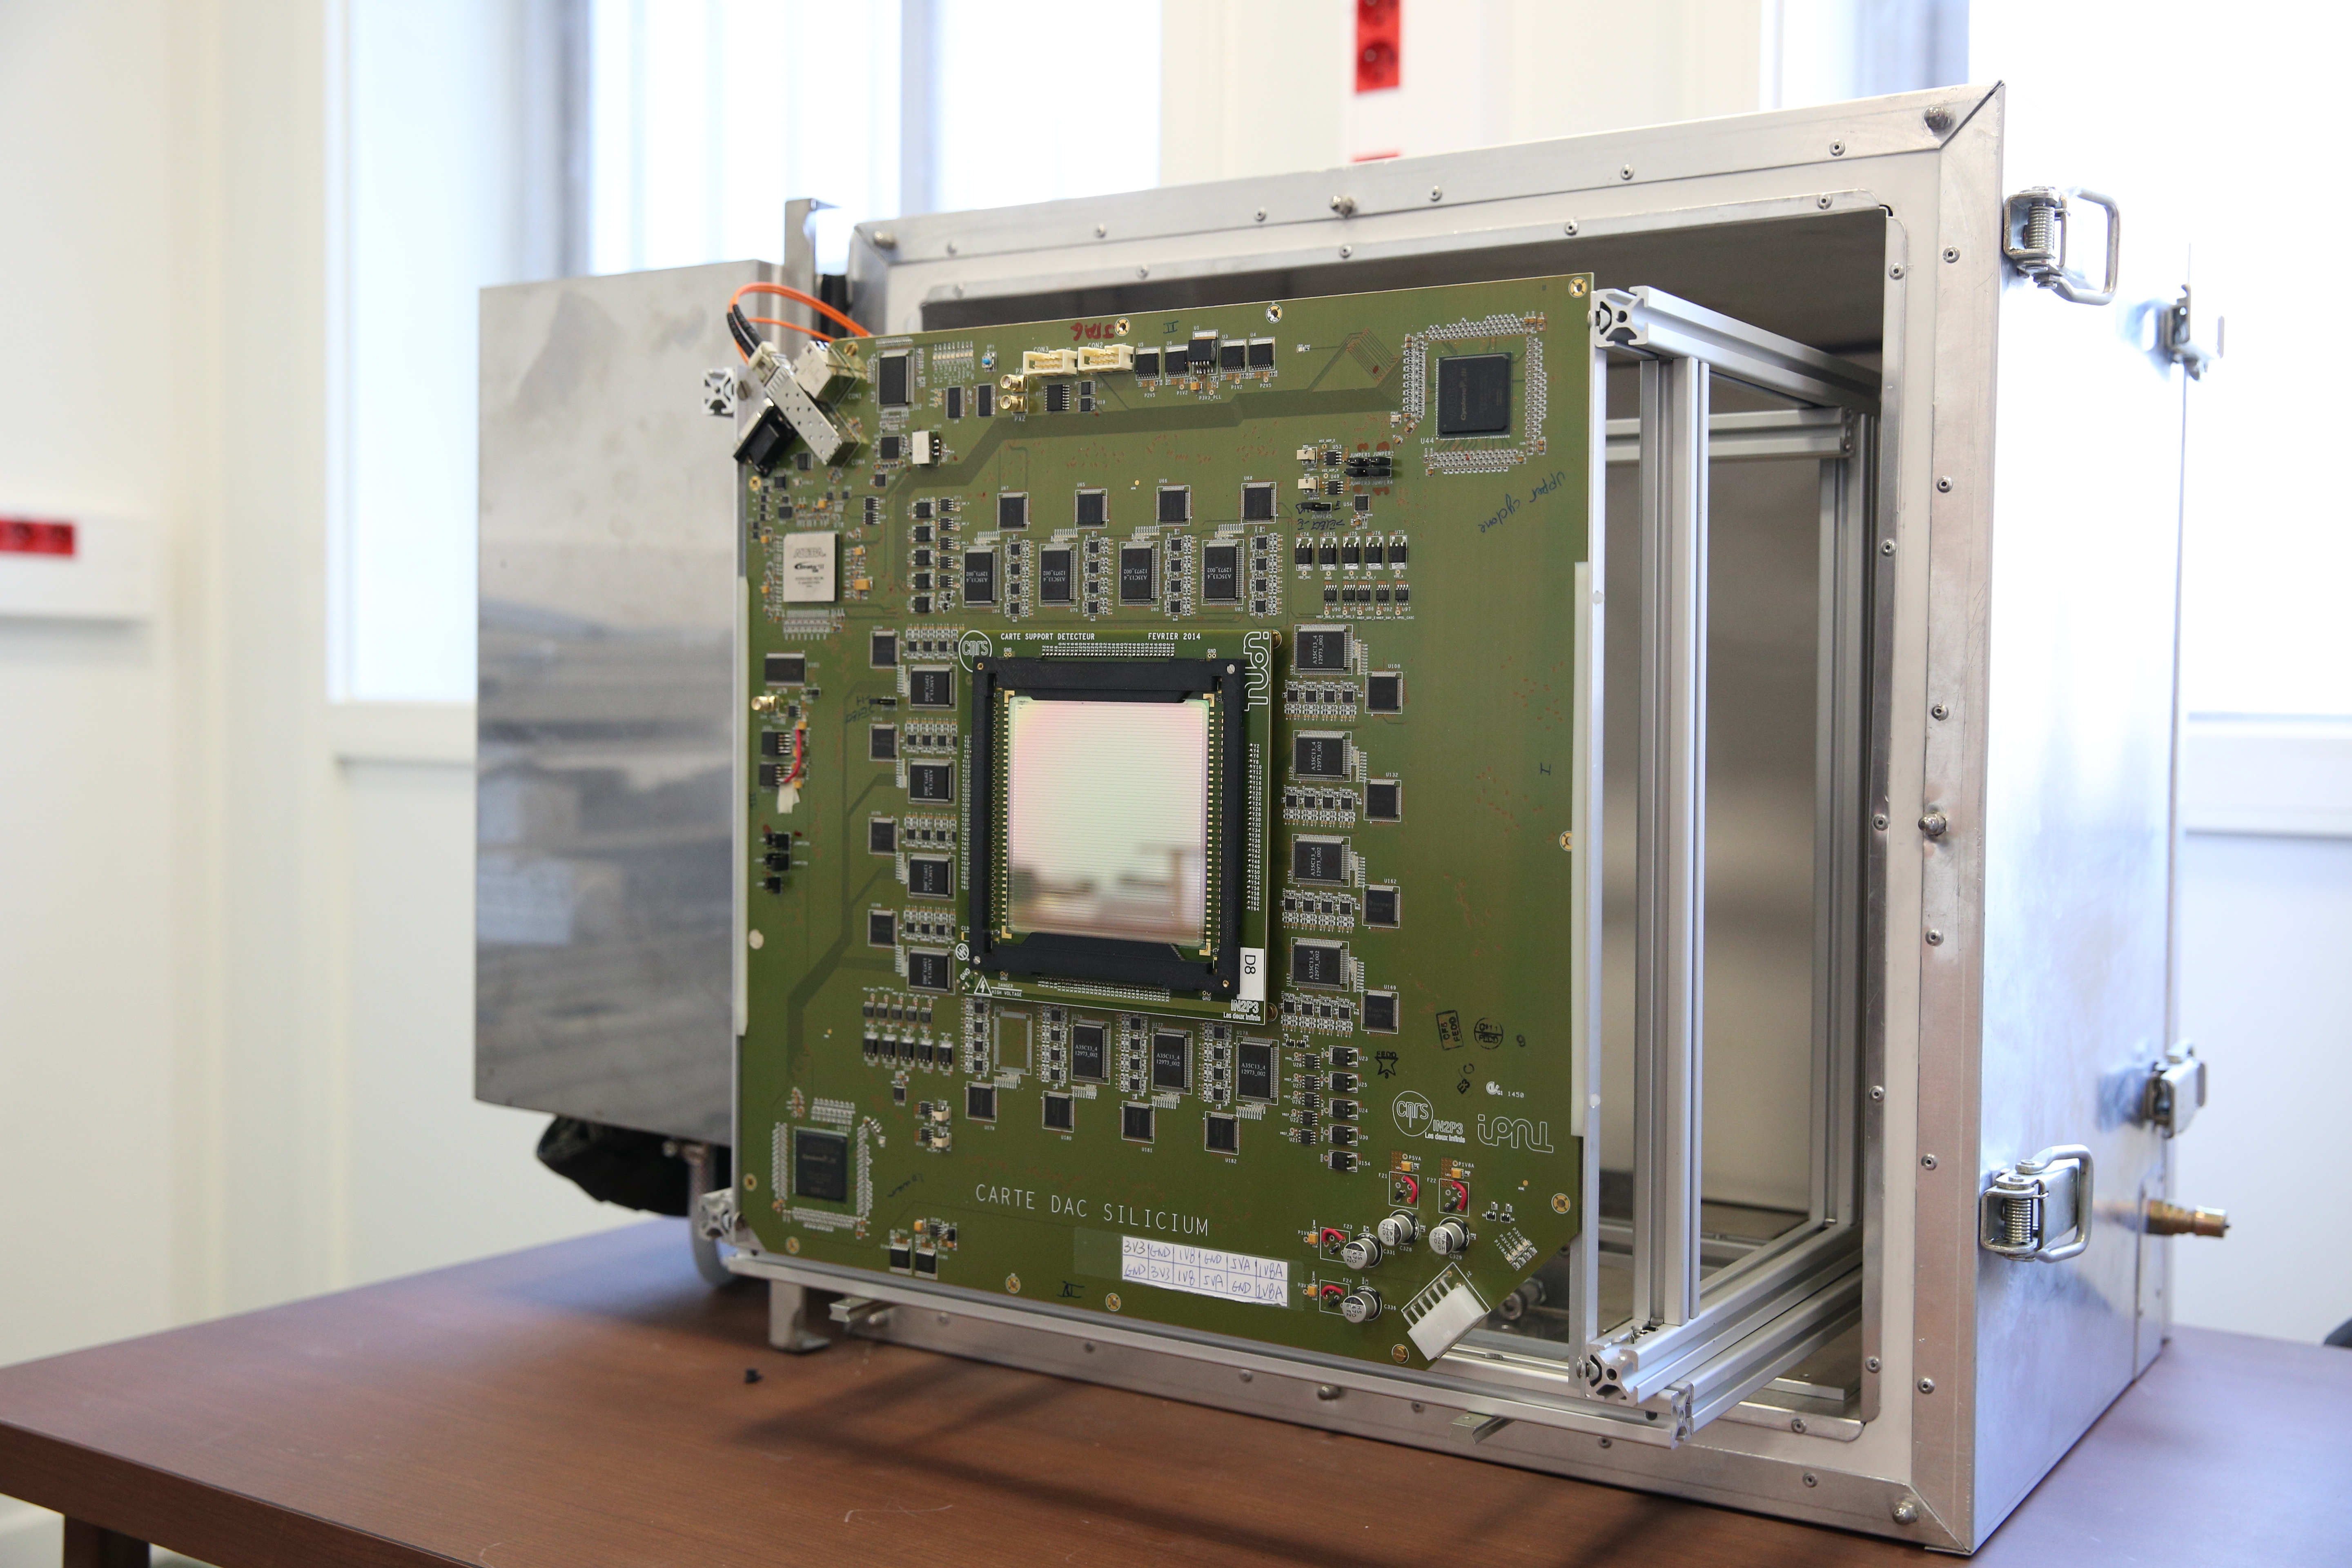
\includegraphics[width=1\textwidth, height=16em]{03_GraphicFiles/chapter3_CLaRySproto/Scatterer/ScattererThermalBox.JPG}
\caption{Scatterer silicon layer with its \gls{fe} card in the thermal regulated box (described in section~\ref{chap3::subsubsec::ScattThermBox}).}
\label{chap3::fig::ScattPicture}
\end{subfigure}
\caption{Overview of the scatterer layers, with its working principle (a) and a picture of the detector connected to the \gls{fe} card in the thermal regulated box (b).}
\label{chap3::fig::scatterer}
\end{figure} 

Each layer has an active volume of 96$\times$96$\times$2~mm$^{3}$, segmented with 64 strips per detection plane. The strip pitch is 1.41~mm, for a strip width of 1.31~mm. The applied polarization voltage is nominally -750~V, and it is uniformly shared on the whole surface to obtain a homogeneous depletion region. A guard ring, composed of 23 strips surrounding the read-out ones on the p side, ensures the desired voltage gradient. The more peripheral strip of the guard ring is connected to the high voltage, while the n side has a single strip for the guard ring, connected to the ground. The p and n read-out strips are then connected to the \gls{fe} electronics via bonding cables.\\
The \gls{fe} electronics card has been developed by the \gls{ipnl} electronics group and is described in details in section~\ref{chap3::subsubsec::ScattFEcard}. The silicon detector is directly plugged on the card, and the mechanical support for the scatterer stack has been studied according to the card size, as shown in \figurename~\ref{chap3::fig::ScattPicture}.\\   
Among the 10 received \glspl{dssd}, only 7 fulfilled the requirements imposed by the Compton camera application, mainly in terms of noise level (leakage current); 3 layer have been rejected, so that the final prototype scatterer is composed of 7 silicon planes.\\
The 7 selected layers have been characterized with a temporary acquisition system in terms of leakage current at different temperatures. The results of these measurements can be found in~\cite{Ley2015}. The measurements allowed to verify the producer specifications in terms of polarization voltage to be applied for a complete detector depletion, as well as to identify the noisy strips and create a complete characterization database. In addition to this, they highlighted the need to cool the detectors down with respect to the room temperature (25\textdegree{}C) in order to reduce the leakage current to acceptable levels, and so reducing the total noise level, affecting the detector performance. In order to accomplish the cooling task and respect, at the same time, the clinical restrictions, a thermal regulated box based on cold air pump has been designed and produced. It operates as the scatterer stack mechanical support, and it is described in section~\ref{chap3::subsubsec::ScattThermBox}.\\
      
 

\subsubsection{Scatterer Front-End card}\label{chap3::subsubsec::ScattFEcard}
As mentioned in the previous paragraph, the main requirement for the scatterer detector modules is a very good energy resolution. The desired working performance can be quantified as follows:
\begin{itemize}
\item 1~keV \gls{fwhm} energy resolution;
\item 1.41~mm spatial resolution (corresponding to the strip pitch);
\item 15~ns \gls{fwhm} time resolution.
\end{itemize} 

The scatterer \gls{fe} card has been developed by the \gls{ipnl} electronics group in order to achieve this performance. It is composed of two well separated sections, analog and digital, which must be kept separated in the card layout in order to minimize the contribution of the digital noise on the treatment of the analog signals. Moreover, in order to reduce the electronic noise, the analog section must be placed as close as possible to the detector, to minimize the signal path length.\\
At first, a dedicated \gls{asic} has been designed and developed to treat the signals directly coming from the \gls{dssd}~\parencite{Dahoumane2014}. Each \gls{asic} 
processes 8 detectors channels, so that 8 \gls{asic} per plane are required for the read-out of a complete silicon layer. This section represents the core of the analog stage. The \gls{asic} has been designed and tested to achieve the desired performance in terms of \gls{enc}, which must be lower than 118 electrons \gls{rms} in order to obtain the 1~keV \gls{fwhm} energy resolution, signal dynamics and accepted detection rate. The analog raw signal first passes through a \gls{csa}, which returns an analog amplified signal. This pulse can be further amplified with a \gls{shs} based on a \gls{cr-rc} filter, which filters and shapes the signal in about 1~\charmus, or via a fast amplifier (with 15~ns shaping time). The first mode is used for a refined charge (deposited energy) measurement and can be employed for detector tests and characterization, while the second is the standard working one which allows for fast energy and time measurements. The amplified signal finally passes through a discriminator, which gives a digital output. Analog (from \gls{csa} or \gls{shs}) and digital signals are then sent to the digital stage of the card for the measurement of time, position and energy. To be noticed \\
The digital stage is mainly composed of one \gls{adc} module per \gls{asic} and two \glspl{fpga}. The analog signal from the \gls{asic} is processed by the \gls{adc}, which is a 12-bit module with 8 channels, with a sampling rate of 100~\gls{mpsp}. Each \gls{adc} returns 16 \gls{lvds} pairs (2 per channel), which are sent to the \glspl{fpga} together with two clock signals (two \gls{lvds} pairs) and the 8 digital outputs of the \gls{asic}. So, 44 input channels of the \gls{fpga} are used for the acquisition of 8 read-out channels (one \gls{asic}). Two \glspl{fpga} Altera Cyclone III~\parencite{Altera2012} are installed on the card to handle the signals coming from the whole detector (128 channels, 64 per detection plane): both of them are equipped with a \gls{tdc} for the time measurement.\\
A third \gls{fpga} (Altera StratixII GX~\parencite{Altera2009}) is finally installed on the card to handle the processed data collection and the communication with the acquisition system, described in section~\ref{chap3::subsec::cameraElectronicsDAQ}, via a 3~Gbit/s link.\\
The \gls{asic} has been developed in three versions, and the cards have been optimized during the development process and produced in its final version (shown in \figurename~\ref{chap3::fig::scattDAQcard}) in the spring 2017. The 7 cards are now available and the development of the \gls{fpga} firmware is ongoing.\\
More details about the card layout, components and operating principle, as well as a description of the tests performed during the development can be found in~\cite{Chen2017} and~\cite{Dahoumane2012}.    

\subsubsection{Scatterer thermal regulated box}\label{chap3::subsubsec::ScattThermBox}

The results of the leakage current tests performed on the silicon detectors showed the need of cooling the detector down to achieve the required performance in terms of noise, which affects the spatial, time and energy resolutions. The leakage current has been studied in temperature cycles in the range -40 - +40~\textdegree{}C, and an overall consistent behavior has been observed both on N and P strips of the detector. The leakage current slightly increases in the range -40 - 0~\textdegree{}C, with values in the range 0 - 8~nA for the analyzed strips, and then drastically increases beyond 0~\textdegree{}C, with peaks of more then 80~nA at +40~\textdegree{}C. The complete description of the performed measurements and the detailed results can be found in~\cite{Ley2015}.\\
A cooling system is needed for the silicon detectors operations: it must be able to keep the temperature constant and below, at least, 0~\textdegree{}C, preferably around -20~\textdegree{}C where the leakage current is more stable in case of small temperature variations. The clinical environment limitations must be considered to design such a cooling system (portability, gas, noise level), as well as the material budget and the mechanical integration with the other camera components.\\
The implemented solution consists in the thermal regulated box shown in \figurename~\ref{chap3::fig::ScattPicture}, together with one of the silicon layers. The size of the box is 490$\times$490$\times$300~mm$^3$, and the structure is composed of 2~mm of aluminum and three insulation layers of 10~mm of silica aerogel Spaceloft\textsuperscript{\textregistered}~\parencite{Spaceloft2011}, for an equivalent thickness of 2~mm of silicon (0.7\% of interaction probability for 1~MeV photons). The cooling is performed via an electric air pump, which is able to keep the temperature inside the box at -20~\textdegree{}C with a 400~W haet evacuation power. The heat power produced by the 7 silicon \gls{fe} cards in operation must be verified, but the estimate confirms the effectiveness of the thermal box nominal performance. Once card and detector will be fully operational, a test will be performed to check the temperature stability inside the box.\\
The 	\gls{fe} cards and the silicon layers are fixed inside the box via a mechanical support designed and produced by the \gls{ipnl} mechanics group. The support, which ensures a millimeter position accuracy, is fixed on metal rails which allow to easily handle each detector layer. A scheme of the thermal box and the internal support is shown in \figurename~\ref{chap3::fig::thermalBox}.
    
\begin{figure}
\begin{subfigure}[t]{.5\textwidth}
\centering
\includegraphics[width=1\textwidth, height = 5.7cm]{03_GraphicFiles/chapter3_CLaRySproto/Scatterer/DAQ_card.JPG}
\caption{Final version of the scatterer \gls{fe} card with the silicon detector layer.}
\label{chap3::fig::scattDAQcard}
\end{subfigure}
\begin{subfigure}[t]{.5\textwidth}
\centering
\includegraphics[width=1\textwidth, trim={5cm 0 5cm 0}, clip = true, height = 5.7cm]{03_GraphicFiles/chapter3_CLaRySproto/Scatterer/Rack_cartes_Si_2.jpg}
\caption{Scheme of the scatterer stack thermal box and internal mechanical support.}
\label{chap3::fig::thermalBox}
\end{subfigure}
\caption{Scatterer silicon layers equipment: final version of the \gls{fe} card (a) and scheme of the detector integration in the thermal regulated box (b).}
\label{chap3::fig::scattererCardMech}
\end{figure} 

%%%%%%%%%%%%%%%%%%%%%%%%%%%%%%%%%%   COLLIMATOR  %%%%%%%%%%%%%%%%%%%%%%%%%%%%%%%%%%%%%%%%%%%%

\subsection{Collimator}\label{chap3::subsec::collimator}
 
The multi-collimated camera is equipped with a multi-slit collimator, with tungsten slabs. Its design has been extensively studied in Monte Carlo simulations~\parencite{Pinto2014}, and it can be easily adapted to different geometrical configurations of the absorber detector and to various monitoring requirements. In particular, the distance between neighboring slabs can be modified, as well as the number of total slabs, in order to find the best trade-off between detection efficiency and spatial resolution; this depends on the distance patient-collimator, on the required extension of the field of view and on the desired monitoring time. Two identical collimators of 30$\times$14$\times$17~cm$^{3}$ have been produced, in order to be able to set several absorber configurations in the transverse direction (extended version along the beam axis or in the perpendicular direction). In \figurename~\ref{chap3::fig::collimatorPicture} a picture of the tungsten collimator is presented, while in \figurename~\ref{chap3::fig::collimatorScheme} we show a schematic view of a possible multi-collimated camera configuration.\\

\begin{figure}
\begin{subfigure}[t]{.5\textwidth}
\centering
\includegraphics[width=\linewidth, trim={0 0 0 0.5cm},clip = true, height = 5cm]{03_GraphicFiles/chapter3_CLaRySproto/Collimator/Collimator.pdf}
\caption{Multi-slit tungsten collimator.}
\label{chap3::fig::collimatorPicture}
\end{subfigure}
\begin{subfigure}[t]{.5\textwidth}
\centering
\includegraphics[width=\linewidth, trim={3cm 0 0 0},clip = true, height = 5cm]{03_GraphicFiles/chapter3_CLaRySproto/schemes/AbsoberCollimator.jpg}
\caption{Scheme of the multi-slit collimated camera configuration.}
\label{chap3::fig::collimatorScheme}
\end{subfigure}
\caption{Tungsten collimator and its setup in the multi-slit collimated camera. The two tungsten multi-slit collimators are placed in front of a 6$\times$5 \gls{bgo} block absorber setup in its mechanical support (see section~\ref{chap3::subsec::absorber}).}
\label{chap3::fig::collimatorFig}
\end{figure} 


%%%%%%%%%%%%%%%%%%%%%%%%%%%%%%%%%%   ABSORBER  %%%%%%%%%%%%%%%%%%%%%%%%%%%%%%%%%%%%%%%%%%%%

\subsection{Absorber}\label{chap3::subsec::absorber}

The Compton and multi-collimated camera absorber was initially conceived as a very large surface plane composed of 96 \gls{bgo} blocks recovered from a dismantled \gls{pet} system HR+ by SIEMENS, documented in~\parencite{Adam1997, Brix1997}.\\ 
%%%From BGO paper %%%%%%%%
\gls{bgo} is one of the most used scintillators for gamma detection applications, thanks to a good energy resolution and a optimal gamma detection efficiency. Moreover, the absence of internal radioactivity which characterizes other scintillator materials employed in the same field (i.e.~\gls{lyso}, \gls{lso}), makes it suitable for low noise detectors, required by a Compton camera to reduce the amount of random coincidences, one of the main sources of background for the application in ion beam therapy monitoring~\parencite{Ortega2015}. As highlighted in~\parencite{HuesoGonzalez2015}, \gls{lyso} and \gls{lso} show overall better performances with respect to \gls{bgo} for what concerns energy, time and spatial resolution, due to an about 4 times higher light yield, but the gap is reduced for the detection of gamma rays in the prompt-gamma energy range (especially beyond 1~MeV). The limited cost of \gls{bgo} with respect to \gls{lso} and the comparable performances in the prompt-gamma energy range make it an optimal solution for prompt-gamma camera prototypes.\\
Each \gls{bgo} block has a surface of 3.5$\times$3.8~cm$^2$, with a thickness of 3.0~cm. The mono-block \gls{bgo} crystal is streaked in a 8$\times$8 pseudo-pixel matrix; a reflecting material is inserted between the pseudo-pixels to improve the light collection and optimize the spatial information accuracy via pixel separation. The read-out is achieved via four \gls{pm} tubes per block, composing a quartet, coupled to the block back surface. Thanks to the internal streaked structure of the block, the scintillation light is shared on the four \glspl{pm} depending on the pseudo-pixel where the interaction takes place (in case of multiple interactions more than 1 pseudo-pixel can be involved). The streaks have a different thickness according to their position in the block: they fully cover the block thickness on the block borders and they progressively shorten towards the block center, with a mono-block structure in the central block section on the entrance face. The reconstruction of the position of interaction is done via Anger logic, i.e.~with a center of gravity calculation.\\
The whole set of recovered blocks was supposed to undergo a \enquote{reconditioning} process, including the \gls{pm} removal, the crystal back surface polishing with diamond-based abrasive tool, the single \glspl{pm} gain characterization and grouping in quartets with similar gains, the final re-coupling of the \glspl{pm} and block shielding.\\ A set of \enquote{reconditioned} blocks have been tested with the method described in section~\ref{chap3::sec::charMeasurements} and their performance have been compared to a set of original blocks. An overall degradation of the detection performance has been verified on all the tested \enquote{reconditioned} blocks, which showed lower amplitude output signals probably link to a reduction of the collected scintillation light. Various correction methods have been tested, with unsatisfactory results. According to the outcome of these tests, summarized in~\cite{Sandjong2017}, the collaboration finally opted to adapt the camera design for the use of original, \enquote{non-reconditioned} \gls{bgo} blocks.\\    
Thirty original blocks are now available to compose the absorber detector. In addition to the already presented features, it must be noticed that the lateral surfaces of the original blocks, as well as the half of the \gls{pm} length, are covered by a reflecting material which ensures the complete collection of the scintillation light. This is probably a component which was not well reproduced during the reconditioning process. The whole structure is then protected by a 1~mm thick aluminum foil, which also isolates from external light contamination.\\
\figurename~\ref{chap3::fig::block_noPM} shows one \gls{bgo} block before the coupling to the \gls{pm} quartet: the streaked structure is clearly visible, as well as the white reflecting material separating the pseudo-pixels and the one surrounding the block lateral sides. As mentioned, the same material also covers part of the photo-multiplier tubes, as shown in picture~\ref{chap3::fig::originalBlock_noAl}, where the four \glspl{pm} are glued to the block back surface. The described aluminum cover is visible in \figurename~\ref{chap3::fig::originalBlock_withAl}, while in \figurename~\ref{chap3::fig::BGOblockScheme} a scheme of a block together with the related \gls{pm} quartet is given. The spatial reconstruction logic is also reported in the same figure. To be noticed that the streaked structure of the pseudo-pixels depends on their position in the block: the reflecting streak covers about three fourth of the block thickness for the for the lateral pseudo-pixels, while it is limited to half of the block thickness for the central ones.\\ 

\begin{figure}
\begin{subfigure}[t]{.5\textwidth}
\centering
\includegraphics[width=1\textwidth, height=16em]{03_GraphicFiles/chapter3_CLaRySproto/Absorber/images/block_noPM}
\caption{\gls{bgo} block with its pseudo-pixel internal structure.}
\label{chap3::fig::block_noPM}
\end{subfigure}
\begin{subfigure}[t]{.5\textwidth}
\centering
\includegraphics[width=1\textwidth, height=16em]{03_GraphicFiles/chapter3_CLaRySproto/Absorber/images/originalBlock_noAluminum}
\caption{\gls{bgo} crystal coupled to \gls{PM} quartet and covered with white reflecting material.}
\label{chap3::fig::originalBlock_noAl}
\end{subfigure}\newline
\begin{subfigure}[t]{.5\textwidth}
\centering
\includegraphics[width=1\textwidth, height=16em]{03_GraphicFiles/chapter3_CLaRySproto/Absorber/images/originalBlock_withAluminum}
\caption{\gls{bgo} complete module with aluminum cover.}
\label{chap3::fig::originalBlock_withAl}
\end{subfigure}
\begin{subfigure}[t]{.5\textwidth}
\centering
\includegraphics[width=1\textwidth, height=16em]{03_GraphicFiles/chapter3_CLaRySproto/Absorber/block_scheme.pdf}
\caption{Scheme of a \gls{bgo} block and its spatial reconstruction logic.}
\label{chap3::fig::BGOblockScheme} 
\end{subfigure}
\caption{Components of an absorber module and its working principle.}
\label{chap5::fig::BGO_block}
\end{figure}


\subsubsection{Absorber Front-End and read-out cards}\label{chap3::subsubsec::AbsorberFEcard}

A custom front-end card has been designed and produced by the \gls{lpc} research group \gls{avirm} and is used for the read-out of each \gls{bgo} block. The card is equipped with four voltage modulators which divide the provided high voltage on the 4 photo multiplier tubes. The voltage sent to each \gls{pm} can be mechanically tuned via screw-potentiometers on these modules. A $\varpm$~5~V low voltage is applied to the cards as supply for the differential amplifier modules, one per \gls{pm}. Differential output channels are used to send the \gls{pm} signals to the read-out card, called \gls{asm} board, via flat cables. A picture of the \gls{fe} card is given in \figurename~\ref{chap3::fig::FEcard}. To be noticed that four analog output channels has been added on some cards in order to allow laboratory tests with a signal treatment based on standard electronics modules, as described in section~\ref{chap3::sec::charMeasurements}. These outputs retrieve the signal before the differential amplification stage.\\ 

\begin{figure}
\begin{subfigure}[htbp]{0.5\textwidth}
\centering
\includegraphics[width=\linewidth, angle = -90]{03_GraphicFiles/chapter3_CLaRySproto/Absorber/images/FEcard}
\caption{\gls{fe} card of the absorber \gls{bgo} detectors. 4 analog outputs have been added for test purpose.}
\label{chap3::fig::FEcard} 
\end{subfigure}
\begin{subfigure}[htbp]{0.5\textwidth}
\centering
\includegraphics[width=0.89\linewidth,]{03_GraphicFiles/chapter3_CLaRySproto/Absorber/ASMcard.jpg}
\caption{\gls{asm} board of the absorber \gls{bgo} detectors. Each board performs the read-out of 6 blocks.}
\label{chap3::fig::ASMcard} 
\end{subfigure}
\caption{Absorber read-out electronics: \gls{fe} card (a) and \gls{asm} board (b).}
\label{chap5::fig::AbsorberCards}
\end{figure}

The \gls{pm} signals amplified by the \gls{fe} card are received by the \gls{asm} boards. Developed by the \gls{lpc} \gls{avirm} group, it is based on the \gls{vme} standard and designed for the application in the \gls{dpga} \gls{pet} system, equipped with \gls{lyso} mono-crystals, grouped in quartets and read-out by the same \gls{fe} card described above. The adaptation to the gamma camera application, so that for the \gls{bgo} modules signal treatment, involves only the firmware part, while the design of the board is unchanged. Each board has 24 differential inputs and it is so able to read the signals from 6 \gls{bgo} blocks; a total of 5 boards are then needed for the complete read-out of the gamma camera absorber (30 blocks). The incoming signals are treated by three intermediate cards  equipped with a \gls{drs}4 chip~\parencite{Ritt2009}, designed and developed at the \gls{psi}, with 8 sampling channels at a maximum frequency of 5~\gls{gsps} (200~ps) for 1024 samples, and an \gls{adc} 12~bit-20~MHz module. The sampling frequency of the \gls{drs}4 can be modified to fit with the specific application: in particular, the \gls{bgo} blocks produces wider signals with respect to the \gls{lyso} crystals of the \gls{dpga}. A \gls{fpga} Altera Cyclone IV GX~\parencite{Altera2016} receives and handles the digital outputs of the three intermediate cards and is in charge of sending the date to the acquisition system via a 3~Gbit/s optical link. The \gls{fpga} also governs the generation of the pre-trigger signal which is sent to an auxiliary board called \gls{thor} in order to start the acquisition of the gamma cameras, as detailed in section~\ref{chap3::subsec::cameraElectronicsDAQ}.\\

\underline{Absorber acquisition with development card} \\

During the development of the final camera acquisition system based on the \gls{utca} equipment, which required a dedicated firmware development ad testing process, a temporary acquisition system has been set for the absorber \gls{bgo} blocks, mainly dedicated to the test and characterization of the \gls{asm} boards. It is based on a development commercial electronics card, provided by Terasic (Altera University Program), equipped with an \gls{fpga} Altera Cyclone V~\parencite{Terasic2015}. The card \gls{fpga} can be programmed for the needed tasks, and it is directly connected to an acquisition PC via Ethernet cable. Three \gls{hsmc} connectors allows for the connection to an expansion board SFP-HSMC~\parencite{Terasic2009}, again by Terasic (Altera University Program), provided with a second \gls{fpga} and with optical fiber input/output connectors for the interface to the \gls{asm} boards. A single optical input is configured for this acquisition setup, with the firmware developed by the \gls{avirm} group in \gls{lpc} and adapted at the \gls{ipnl}; one single \gls{asm} card can be connected to the board, so that a maximum of 6 \gls{bgo} block can be read-out at the same time. A picture of the development card connected to the mezzanine is given in \figurename~\ref{chap3::fig::absDevelcard}. \figurename~\ref{chap3::fig::softDevelCard} shows an example of the user interface and data visualization of the C++ based acquisition software developed and provided byt the \gls{avirm} group.   

\begin{figure}
\begin{subfigure}[htbp]{0.5\textwidth}
\centering
\includegraphics[width=0.75\linewidth, angle = 90]{03_GraphicFiles/chapter3_CLaRySproto/Absorber/develCard_zoom.jpg}
\caption{Altera development card for the absorber \gls{bgo} detectors.}
\label{chap3::fig::absDevelcard} 
\end{subfigure}
\begin{subfigure}[htbp]{0.5\textwidth}
\centering
\includegraphics[width=\linewidth]{03_GraphicFiles/chapter3_CLaRySproto/Absorber/ASMcard.jpg}
\caption{Example of acquisition software interface for the absorber \gls{asm} card acquisition base on the Altera development card.}
\label{chap3::fig::softDevelCard} 
\end{subfigure}
\caption{Details of the temporary absorber acquisition based on the Altera development card.}
\label{chap5::fig::AbsorberDevelCards}
\end{figure}

         
 

\subsubsection{Absorber mechanical support}\label{chap3::subsubsec::AbsorberMechanics}

A first mechanical structure for the absorber detector was initially conceived by the \gls{lpc} group in order to hold up to 100 modules, foreseen by the original camera design. The reduction of the number of available blocks caused by the \enquote{reconditioning} process failure make necessary an adaptation of such a support. The new design has been carried out by the mechanics group of the \gls{ipnl} in order to be compact and flexible in terms of detection modules setup. \figurename~\ref{chap3::fig::absorber_scheme} displays both a picture and a scheme of the absorber configuration with its mechanical support. The two lateral sides are built with \gls{pmma} boards connected by metal bars, and the \gls{bgo} blocks can be arranged in up to 5 rows of variable size, ranging from 3 to 7 blocks. Each block row is supported by a thin metal foil, designed to reduce at minimum the blocks separation and to respect the original ring geometry deriving from the SIEMENS \gls{pet} system. The blocks composing a row are then laterally pressed via two screws on the two sides of the structure, which can also be used to adapt the rows relative position horizontally. On the back side, a metal bar is added to avoid undesired movements, and the \gls{fe} cards are fixed with plastic pillars. The realized support results to be versatile, compact and adapted to the prototype tests for both the Compton camera (where a squared setup is preferred) and the multi-collimated one (where the collimator geometry must be fit by the absorber geometrical configuration).       

\begin{figure}
\begin{subfigure}[b]{.5\textwidth}
\centering
\includegraphics[width=1\textwidth, height=16em]{03_GraphicFiles/chapter3_CLaRySproto/Absorber/images/absorber_picture.JPG}
\caption{Picture of the absorber detector in its mechanical support.}
\label{chap3::fig::absorberPicture}
\end{subfigure}
\begin{subfigure}[b]{.5\textwidth}
\centering
\includegraphics[width=1\textwidth, height=16em]{03_GraphicFiles/chapter3_CLaRySproto/Absorber/images/Absorbeur.jpg}
\caption{Scheme of the absorber detector with its mechanical support.}
\label{chap3::fig::absorber30Scheme}
\end{subfigure}
\caption{Absorber front view with the \gls{bgo} block lines arranged in the mechanical support (a). Scheme of the \gls{bgo} absorber with its mechanical support (b).}
\label{chap3::fig::absorber_scheme}
\end{figure}

%%%%%%%%%%%%%%%%%%%%%%%%%%%%%%%%%%   HODOSCOPE  %%%%%%%%%%%%%%%%%%%%%%%%%%%%%%%%%%%%%%%%%%%%

\subsection{Beam tagging hodoscope}\label{chap3::subsec::hodoscope}

A beam tagging hodoscope is being developed in parallel to the two gamma cameras, mainly for background rejection and reconstruction optimization purposes [CIT]. As already mentioned, the detection of prompt-gammas (with mechanical or \enquote{electronical} collimation), is affected by the presence of other secondary particles produced during the ion beam irradiation, mainly neutrons. This background source can be efficiently identified and removed my applying \gls{tof} selection windows to the data acquisition. The \gls{tof} measurements can be performed using the accelerator radio-frequency signal as reference, but a direct beam detection results to be more accurate. An auxiliary detector is then needed before the beam interaction in the patient.\\ 
The \gls{clarys} hodoscope prototype is designed to provide space and time information about the incoming primary beam, particle by particle or bunch by bunch, depending on the beam intensity and detector efficiency and rate acceptance which must be characterized. In addition to the already explained use of the time information, a space primary particle tagging can be used to improve the reconstruction accuracy and constraint the possible reconstructed emission vertex in case of analytic reconstruction approach for both the multi-collimated and Compton cameras (see chapter~\ref{chap::2}).\\  
The detector under development is based on squared 1~mm$^{2}$ polystyrene scintillating fibers BCF-12, 140~mm in length, provided by Saint Gobain~\parencite{SaintGobain2017}. A picture of the hodoscope on its mechanical support (detailed in the following) is presented in \figurename~\ref{chap3::fig::HodoscopeMain}. The fibers are arranged into two perpendicular planes for a two-dimensional spatial information: each plane is composed of 128 fibers, for a total active area (for 2D measurements in coincidence) of 128$\times$128~mm$^{2}$. The active detector surface is completely covered with black reflective tape, which shields from external light. The scintillation light produced in the fibers by a ionizing particle deposing energy is transported to the read-out system via FORETEC optical fibers (1.55~cm diameter, 1~m length), which are connected to the scintillating fibers thanks to a custom mechanical support and to a proper gluing process (see \figurename~\ref{chap3::fig::HodoMounting}). Each scintillating fibers is read-out on both sides to optimize the detector efficiency and improve the time resolution which is not depending on the interaction position along the fiber with this configuration, so that the total number of read-out channels is 512. The signal read-out is ensured by 8 multi-anode \glspl{pm} Hamamatsu H8500~\parencite{Hamamatsu2006} shown in \figurename~\ref{chap3::fig::PMH8500}. The optical fibers are connected to the \gls{pm} anode surfaces through a plastic custom mask, shown in \figurename~\ref{chap3::fig::PMmask}. The \glspl{pm} are equipped with custom black boxes which operate as mechanical support and external light protection (see \figurename~\ref{chap3::fig::HodoMounting}). In order to provide further light isolation, the whole \gls{pm} boxes are covered with black tape.\\
The optical fibers are connected to the \glspl{pm} with the aim of increasing the maximum counting rate. 4 \glspl{pm} are dedicated to the read-out of the horizontal fibers, and 4 to the vertical ones, and the neighboring fibers are connected to different \glspl{pm}. An active area of 4$\times$4~mm$^{2}$ on the two planes is then read-out by all the 8 \glspl{pm}. Moreover, the two sides of the same scintillating fiber are connected on the same \gls{pm}. This fiber connection logic also improve the detector robustness; in case of problem on one \gls{pm}, only 1~mm each 4~mm is lost on a single plane, so that the detection of the beam is still possible on the whole active area.\\  
Each \gls{pm} is connected to a single custom \gls{fe} card. The hodoscope \gls{fe} cards have been developed by the \gls{ipnl} electronics group: their design is described in section~\ref{chap3::subsubsec::HodoFEcard}. 8 \gls{fe} cards are then used for the read-out, and the collected data are sent to the acquisition system described in section~\ref{chap3::subsec::cameraElectronicsDAQ}.

\begin{figure}[!htbp]
\centering
\includegraphics[width=0.6\textwidth]{03_GraphicFiles/chapter3_CLaRySproto/Hodoscope/Hodoscope_onTable.jpg}
\caption{128$\times$128 scintillating fiber hodoscope on its 2-dimensional moving support.}
\label{chap3::fig::HodoscopeMain}
\end{figure}

\begin{figure}
\begin{subfigure}[t]{0.5\textwidth}
\centering
\includegraphics[width=1\textwidth]{03_GraphicFiles/chapter3_CLaRySproto/Hodoscope/Hodoscope_mounting.jpg}
\caption{Scintillating fiber hodoscope during mounting process.}
\label{chap3::fig::HodoMounting}
\end{subfigure}
\begin{subfigure}[t]{0.5\textwidth}
\centering
\includegraphics[width=1\textwidth]{03_GraphicFiles/chapter3_CLaRySproto/Hodoscope/hodoPMfiberConnection.pdf}
\caption{Scheme of the scintillating fiber connection to the \glspl{pm} (top) and of the double-sided fiber read-out (bottom).}
\label{chap3::fig::HodoPMfiberConn}
\end{subfigure}
\newline
\begin{subfigure}[t]{0.5\textwidth}
\centering
\includegraphics[width=1\textwidth, height = 6cm]{03_GraphicFiles/chapter3_CLaRySproto/Hodoscope/H8500.png}
\caption{Hodoscope read-out \glspl{pm} Hamamatsu H8500.}
\label{chap3::fig::PMH8500}
\end{subfigure}
\begin{subfigure}[t]{.5\textwidth}
\centering
\includegraphics[width=1\textwidth, trim = {0 3cm 0 5cm}, clip = true, height = 6cm]{03_GraphicFiles/chapter3_CLaRySproto/Hodoscope/Hodoscope_PMmask.JPG}
\caption{\gls{pm} plastic mask for optical fiber connection.}
\label{chap3::fig::PMmask}
\end{subfigure}
\caption{Details of the scintillating fiber hodoscope setup.}
\label{chap3::fig::HodoscopeParts}
\end{figure}


\subsubsection{Hodoscope Front-End card}\label{chap3::subsubsec::HodoFEcard}

The hodoscope is designed to tag in space and time the incoming beam ions, so that the signal read-out must be optimized to provide accurate time measurements and an high detection rate acceptance, with reduced dead time and detection efficiency close to 100\%. In particular, the design requirements include a maximum counting rate acceptance of 10$^{8}$~Hz per detection plane, with a time resolution of 1~ns~\parencite{Krimmer2014}.  The hodoscope \gls{fe} card shown in \figurename~\ref{chap3::fig::HodoscopeFEcard} has been developed by the \gls{ipnl} electronics group to fulfill the listed requirements. The Hamamatsu \gls{pm} is connected to the 64-channel connector (4 connectors of 16 channels each) and two custom \glspl{asic} are dedicated to the data first treatment (32 channels each).\\
  
\begin{figure}
\centering
\begin{subfigure}[t]{.34\textwidth}
\centering
\includegraphics[width=\linewidth, height = 6cm]{03_GraphicFiles/chapter3_CLaRySproto/Hodoscope/HodoCard1.jpg}
\caption{Hodoscope \gls{fe} card.}
\label{chap3::fig::HodoscopeFEcard}
\end{subfigure}
\begin{subfigure}[t]{.56\textwidth}
\centering
\includegraphics[width=\linewidth, trim = {0 0 1cm 0}, clip = true, height = 6cm]{03_GraphicFiles/chapter3_CLaRySproto/Hodoscope/HodoScheme.png}
\caption{Hodoscope mechanical support scheme.}
\label{chap3::fig::HodoscopeSchemeMech}
\end{subfigure}
\caption{HODOPIC board (a) and scheme of the beam-tagging hodoscope two-dimensional moving support (b).}
\label{chap3::fig::HodoPic}
\end{figure}

A first version of the \gls{fe} \gls{asic} has been developed in 2012 by the group \gls{micrhau} for the read-out of 8 channels (designed for the 32$\times$32 fiber hodoscope prototype described in section~\ref{chap3::subsubsec::SmallHodoProto}). The input part is composed of a current conveyor, and the output one has two sections: a current discriminator and a charge pre-amplifier for the charge measurements in test mode~\parencite{Deng2012, Deng2013}. In addition, the \gls{asic} gain can be tuned channel by channel, so that the response of each \gls{pm} output channel can be fine tuned with respect to the others.\\
The second version of the \gls{asic} includes all the features of the first version, with the addition of a \gls{tdc} based on a 160~MHz clock for a more accurate time tagging of the detected events. Moreover, a \gls{dll} is installed to divide the main clock in 32 intervals: for each event, the \gls{dll} state is stored in a 32 bit register and then encoded in a 5-bit Gray decoder. As a result, the \gls{tdc} has a 6.25~ns dynamics, with a sampling step of 195~ps and a time resolution of 58.8~ps \gls{rms}, for a maximum accepted rate of 10$^{8}$~Hz~\parencite{Deng2012b}.\\
The third and final \gls{asic} version, called HODOPIC, is adapted to the big size hodoscope (512 read-out channels), with the extension to 32 channels and with the \gls{tdc} implemented on the second version. An external \gls{adc} is used for the charge measurement in test mode for a single channel, selected via slow control. All the \gls{asic} outputs are sent to a \gls{fpga} installed on the card for the actual time measurement and data decoding. The \gls{fpga} finally handles the data transmission to the acquisition system, depending on the card version.\\
A first card has been developed to test the first \gls{asic} version with the 32$\times$32 fiber hodoscope. It is based on a \gls{fpga} Altera Cyclone III~\parencite{Altera2012} and on 9 \glspl{asic}, with a LabVIEW acquisition. A single card is enough for the read-out of the complete small hodoscope prototype. This first setup has been tested on beam at the \gls{ganil} and the \gls{hit}, and a sub-ns time resolution has been verified, together with the expected 1~mm spatial resolution on the two fiber planes and an efficiency of more then 90\% at a 10$^{6}$ acquisition rate.\\
The second prototype of the card, shown in \figurename~\ref{chap3::fig::HodoscopeFEcard}, has been adapted to the 512-channel hodoscope described in the previous section and to the gamma camera acquisition system described in~\ref{chap3::subsec::cameraElectronicsDAQ}: each card has two HODOPIC \glspl{asic}, 32 channels each, so that it is designed for the read-out of a single 64-anode \gls{pm}. 8 cards are then needed for the read-out of the whole hodoscope. This version is based on a \gls{fpga} Altera StratixII GX~\parencite{Altera2009}, and the connection to the acquisition is ensured by a 3~Gbit/s optical link. 4 digital input-output channels are installed for test and validation purpose, together with an Ethernet port.\\
Further details about the different card versions and the applied validation tests can be found in~\cite{Chen2017}.\\
The hodoscope card firmware has been developed in 2017 and tested in simplified versions on beam, as detailed in chapter~\ref{chap::6}.
           

\subsubsection{Hodoscope mechanical support}\label{chap3::subsubsec::HodoMechanics}

The beam tagging hodoscope is set between the beam nozzle and the patient and requires a dedicated mechanical support. In order to profit of the large active area and to be able to remotely control the hodoscope position in the beam transverse plane, the detector is mounted on a 2-dimensional moving table (see the picture in \figurename~\ref{chap3::fig::HodoscopeMain}), which also supports the \gls{fe} cards. Detector and \gls{fe} cards are then integral and translate together. A scheme of the moving table is given in \figurename~\ref{chap3::fig::HodoscopeSchemeMech}.\\
The 2-axis table is provided by Beijing Winner Optical Instruments; it is composed of two motorized linear stages, connected via a right angle bracket. The two stages have a moving range of 30~cm each and the stepper motors have a step resolution of 20~\charmum. The employed motor controller is a Newport XPS-Q8~\parencite{Newport2017}, equipped with 8 channels for the simultaneous control of a maximum of 8 motors. The movements are steered with an online interface or with a LabVIEW based program, which will be integrated in the final setup of the slow control software under development with the cameras.

\subsubsection{Small hodoscope prototypes}\label{chap3::subsubsec::SmallHodoProto}
Before the production of the large active surface hodoscope prototype described in section~\ref{chap3::subsec::hodoscope}, two smaller prototypes have been produced and tested in order to assess the potential of such a kind of detector for the required application. The first and simplest version consisted of one single scintillating fiber per plane, and the readout was performed with two \gls{pm} tubes directly coupled to the scintillating fibers, without optical fibers. A picture of this prototype is given in \figurename~\ref{chap3::fig::singleFibHodo}. This simple version of the detector has been used as a demonstrator of the basic detection principle.\\ 

\begin{figure}
\begin{subfigure}[t]{.5\textwidth}
\centering
\includegraphics[width=0.8\textwidth]{03_GraphicFiles/chapter3_CLaRySproto/Hodoscope/hodo2.jpg}
\caption{Hodoscope small prototype, 1$\times$1 scintillating fibers.}
\label{chap3::fig::singleFibHodo}
\end{subfigure}
\begin{subfigure}[t]{.5\textwidth}
\centering
\includegraphics[width=0.8\textwidth]{03_GraphicFiles/chapter3_CLaRySproto/Hodoscope/hodo32_withCard.jpg}
\caption{Hodoscope small prototype, 32$\times$32 scintillating fibers, connected to the HODOPIC \gls{fe} board.}
\label{chap3::fig::Hodoscope32}
\end{subfigure}
\caption{Hodoscope small prototypes.}
\label{chap3::fig::HodoSmall}
\end{figure}

A second small size version of the final detector has been produced with almost the same features as the large area prototype but with simplified read-out logic. It is equipped with two perpendicular planes of 32 1~mm$^{2}$ scintillating fibers each (Saint Gobain BCF-10~\parencite{SaintGobain2017}), with a length of 4~cm and a total active area for a 2D read-out of 32$\times$32~mm$^{2}$. As in the big hodoscope, the scintillating fibers are coupled to FORETEC optical fibers which transfer the scintillation light to 4 Hamamatsu H8500 \glspl{pm}. 16 channels per \gls{pm} are used, so that 2 \glspl{pm} are dedicated to the horizontal fibers and 2 to the vertical ones, and the signal read-out is performed on a single side of the scintillating fibers. As the total number of read-out channels is 64, a single \gls{fe} card is enough for the whole detector. In \figurename~\ref{chap3::fig::Hodoscope32} the 32$\times$32-fiber hodoscope prototype is shown together with its \gls{fe} card; 4 connections cables (16 channels each) are used to couple the \glspl{pm} to the \gls{fe} card.\\
The 32$\times$32-fiber hodoscope prototype has been tested in 2014 on proton and carbon ion beams (at the \gls{ganil} - 75~MeV/u $^{13}$C, \gls{hit} - protons and carbon ions at various energy, \gls{ipno} - 25~MeV protons) with the first version of the \gls{fe} card (see section~\ref{chap3::subsubsec::HodoFEcard}): an efficiency of more than 90\% has been retrieved, with a time resolution of 1~ns \gls{fwhm} (timing measurements performed with respect to the accelerator high frequency signal). Some more details about this beam tests results are given in chapter~\ref{chap::6}. The final version of the \gls{fe} card has been also tested with this detector, and the test description and results are presented in chapter~\ref{chap::6}.  
   

%%%%%%%%%%%%%%%%%%%%%%%%%%%%%%%%%%   ELECTRONICS/DAQ  %%%%%%%%%%%%%%%%%%%%%%%%%%%%%%%%%%%%%%%%%%%%

\subsection{Camera acquisition system}\label{chap3::subsec::cameraElectronicsDAQ}

The \gls{tof} gamma cameras developed by the \gls{clarys} collaboration are composed of various detection sections: beam tagging hodoscope and \gls{bgo} absorber for the multi-slit collimated camera, with the addition of the silicon scatterer stack for the Compton camera. The acquisition system must be able to handle the data flux from the different components, for a total of 20 \gls{fe} cards (7 for the silicon scatterer, 8 for the hodoscope and 5 for the absorber), select the events according to the chosen trigger logic and create and send the data packet with the right format to the acquisition PC.\\
The system is based on the \gls{utca} standard; originally conceived as an adaptation of the \gls{atca} systems used in the telecommunication field for high-flux data transfers, it is employed for relatively simpler tasks and adopted in the particle physics domain since less than ten years~\parencite{Cachemiche2012, Abellan2013}. A standard \gls{utca} crate equipped with a \gls{mch} (shown in \figurename~\ref{chap3::fig::uTCAcrate}) is used as general purpose support for the \gls{amc}, which is the section adapted for each specific application. An \gls{amc}40 has been developed for high energy physics applications, in particular for the \gls{lhcb} experiment at \gls{cern}, and has been adapted for the gamma camera acquisition system by the \gls{cppm} research group (see \figurename~\ref{chap3::fig::AMC40}). This card includes a \gls{fpga} Altera Stratix V~\parencite{Altera2015}, 24 optical inputs at 4.8~Gbit/s and 12 at 9.6~Gbit/s, a 1~Gbit/s Ethernet output for the connection to the acquisition PC. In addition to the \gls{utca} based components, an intermediate card in \gls{vme} format completes the acquisition system. The so-called \gls{thor} card (see \figurename~\ref{chap3::fig::THOR}), developed in \gls{vme} format at \gls{lpc} in parallel to the \gls{asm} card, is used to generate and share the clock signal common to the whole electronics cards for synchronization purpose (40~MHz) and to govern the pre-trigger and trigger signals as explained in the following lines.\\  


\begin{figure}
\begin{subfigure}[htbp]{.55\textwidth}
\centering
\includegraphics[width=\linewidth]{03_GraphicFiles/chapter3_CLaRySproto/Electronics_Acquisition/uTCAcrate_1.jpg}
\caption{\gls{utca} crate with the \gls{amc}40 board.}
\label{chap3::fig::uTCAcrate}
\end{subfigure}
\begin{subfigure}[htbp]{.41\textwidth}
\centering
\includegraphics[width=\linewidth, angle = -90]{03_GraphicFiles/chapter3_CLaRySproto/Electronics_Acquisition/AMC40_ipnl_top.jpg}
\caption{\gls{amc}40 board.}
\label{chap3::fig::AMC40}
\end{subfigure}
\newline
\begin{subfigure}[b]{\textwidth}
\centering
\includegraphics[width=0.8\linewidth]{03_GraphicFiles/chapter3_CLaRySproto/Electronics_Acquisition/THOR.pdf}
\caption{\gls{thor} card.}
\label{chap3::fig::THOR}
\end{subfigure}
\caption{Acquisition system components: \gls{utca} crate (a), \gls{amc}40 board (b) and \gls{thor} card (c).}
\label{chap3::fig::AcquisitionSystem}
\end{figure}


For both cameras, the acquisition starts in case the absorber section detects an interaction: the \gls{asm} involved card deals with the creation of a pre-trigger signal, which corresponds to the digital output signal and contains a time stamp (see the \gls{asm} card description in section~\ref{chap3::subsubsec::AbsorberFEcard}). The pre-trigger is sent to the \gls{thor} card who governs its distribution to the other system components.\\ 
In the multi-slit collimated camera, the pre-trigger signal directly operates as a trigger validating the data collection from absorber and hodoscope. In the Compton camera, the \gls{thor} card initially sends the pre-trigger to the scatterer \gls{fe} cards, which explore their buffer looking for events in the coincidence time window; if a coincidence is found, a trigger signal is generated by the scatterer \gls{fe} card and sent to the acquisition system, which then starts the data read-out from all the detectors. An graphical overview of the complete acquisition system and logic is given in \figurename~\ref{chap3::fig::DAQscheme}.\\
The \gls{amc}40 card makes use of three buffers for the three detector sections, where the collected data are stored until the creation of packets of the selected size to be sent to the acquisition PC. The data transfer is achieved via a 1~Gbit/s Ethernet link, and the chosen standard is the \gls{udp}. The data format has been fixed at the camera conception stage and slightly modified following the electronics developments; it is deeply described in the appendix~\ref{chap::appA}, which also reports the expected data flow obtained in previous simulation studies.\\  
In addition to the already explained functions, the \gls{utca} is also in charge of handling the slow control signals for the configuration of the detector \gls{fe} cards. The chosen format is in this case the \gls{tcp}, which is more reliable and ensures a feedback in case of communication failure. The possible slow control signals are detailed in appendix~\ref{chap::appA}.\\

\begin{figure}[!htbp]
\centering
\includegraphics[width=\textwidth, trim = {0 2cm 0 2cm}, clip = true]{03_GraphicFiles/chapter3_CLaRySproto/Electronics_Acquisition/acqLogic_complete.pdf}
\caption{Schematic view of the Compton camera acquisition system. For the multi-collimated camera, the trigger and pre-trigger signals are the same.}
\label{chap3::fig::DAQscheme}
\end{figure}

%%%%%%%%%%%%%%%%%%%%%%%%%%%%%%%%%%   SOFTWARE  %%%%%%%%%%%%%%%%%%%%%%%%%%%%%%%%%%%%%%%%%%%%

\subsection{Camera acquisition, monitoring and slow control software}\label{chap3::subsec::cameraSoftware}

The \gls{udp} data packets sent by the \gls{utca} acquisition system via Ethernet link are received by the acquisition PC thanks to a C++ based acquisition software, developed at the \gls{ipnl}. The software decodes the data packets and builds the events by grouping the data from the two (for the multi-slit collimated camera) or three (for the Compton camera) detection sections according to the time stamp. During the decoding process, the software also verify the received data format and can highlight problems in the data encoding by the \gls{utca}; this feature is used during the test phase to check the functionality of the \gls{amc}40 firmware. The reconstructed events are then stored in binary files with the structure presented in appendix~\ref{chap::appA}. The data file size can be selected by fixing the number of events stored per run in the acquisition run, knowing that each event can be composed by slightly different number of bits, according to the amount of detector modules involved. The file collection corresponding to the same run will be then grouped at the analysis stage. The number of events per file must be tuned taking care of the available \gls{ram} (32~Gb), where the data are temporarily stored before the writing process on the hard-disk. In \figurename~\ref{chap3::fig::daqSoftware} the minimal graphical interface developed for the acquisition software is shown.\\

\begin{figure}
\begin{subfigure}[t]{.5\textwidth}
\centering
\includegraphics[width=0.75\textwidth]{03_GraphicFiles/chapter3_CLaRySproto/Electronics_Acquisition/DAQsoft.png}
\caption{Acquisition software user interface.}
\label{chap3::fig::daqSoftware}
\end{subfigure}
\begin{subfigure}[t]{.5\textwidth}
\centering
\includegraphics[width=1\textwidth]{03_GraphicFiles/chapter3_CLaRySproto/Electronics_Acquisition/monitoringEx.pdf}
\caption{Example of monitoring software visualization for the beam tagging hodoscope (applied to the 32$\times$32 fiber prototype).}
\label{chap3::fig::monitoringSoftware}
\end{subfigure}
\caption{Software tools: user interface of the acquisition C++ software (a) and example of the ROOT monitoring software visualization for the beam tagging hodoscope 32$\times$32 fiber prototype.}
\label{chap3::fig::SoftwareAll}
\end{figure}

A monitoring software has been developed in order to have a direct real-time feedback on the camera data acquisition. The software can show some information about the ongoing data collection, and it is at present designed to work on a single detector section (hodoscope, scatterer or absorber). It is based on ROOT with the following working logic: during the acquisition, it continuously searches for new data files in the storage folder, and analyses in the desired way a selected number of events per file, directly from the binary format. An example of the visualized output for an hodoscope monitoring is shown in \figurename~\ref{chap3::fig::monitoringSoftware}. This picture corresponds to an acquisition performed during a beam test at the \gls{cal}, where the 32$\times$32 fiber hodoscope have been tested, together with the monitoring software. More details about the beam test are given in chapter~\ref{chap::6}.\\ As mentioned, the present version of the software is not yet adapted to the monitoring of the whole camera, even if it can handle at least two detectors with minor modifications. In addition to this, it is not automatically synchronized with the acquisition software, and not optimized in terms of needed calculation time. In the next future the planned upgrade will slightly modify the working logic by directly connection the monitoring to the acquisition: the acquisition software will automatically send a selected fraction of events to the monitoring output during the acquisition, so that the search for data files would not be anymore necessary. This will drastically reduce the monitoring dead time and calculation time, achieving an actual online control.\\
Acquisition and monitoring software has been tested thanks to a data simulator developed in C++, which is able to create data \gls{udp} packets with the correct format and send them on the same Ethernet port used for the data collection, simulating a server-client communication.\\

As mentioned in section~	\ref{chap3::subsec::cameraElectronicsDAQ}, the \gls{utca} handles both the data collection and transfer and the slow-control of the whole system, where with slow-control we intend the configuration of all the electronics cards (discriminator thresholds, channel gains, \gls{asic} reset signals, working mode, etc.) and the read-out of the feedback signals. The development of the slow-control software is ongoing at the \gls{ipnl}: it is designed in LabVIEW and includes all the needed controls in a single user interface. A dedicated PC is foreseen for this task, connected to the \gls{utca} via \gls{tcp} protocol. The slow-control software will also govern the high and low voltage suppliers for the detectors and acquisition electronics boards, the scatterer thermal box temperature setup and control, the steering of the 2D positiong table dedicated to the hodoscope, and the steering of the camera moving table, described in the next section. All the listed instruments will be connected to a patch panel, and a local network will be created for the camera equipment.      

%%%%%%%%%%%%%%%%%%%%%%%%%%%%%%%%%%   MECHANICAL SUPPORT  %%%%%%%%%%%%%%%%%%%%%%%%%%%%%%%%%%%%%%%%%%%%

\subsection{Camera integration and mechanical support}\label{chap3::subsec::CameraMechanics}

In order to setup the two camera configurations (multi-slit and Compton), the described components, together with the related mechanical supports, must be integrated in an integral system, with the exception of the beam tagging hodoscope who has its own dedicated mechanical support, being placed between the beam nozzle and the target. A general mechanical structure is then needed to support the camera; it is required to be movable, as compact as possible but at the same time robust and large enough to support absorber and scatterer (or collimator), for a total maximum weight of about 100~Kg. In addition to this, it should be possible to remotely control the position of the various camera components in order to adapt their position in 3D with respect to the beam line and to the target.\\
The realized solution is shown in \figurename~\ref{chap3::fig::pictureTable}. It is composed of two sections: a positioning table on wheels, designed and provided by Rose \& Krieger, equipped with 4 telescopic feet, and a 4-axis moving table installed on it, developed by Kinetic System. The wheels allow to first position the camera, and the 4 telescopic feet are used to regulate with 1~mm precision the whole system height, in the range 630~mm - 1280~mm from the ground, to be adapted to the specific beam line. The feet are expected to be able to support a maximum weight of 150~Kg. The telescopic feet are not connected to the slow-control but are controlled by a remote controller on the table itself. On the top surface of the table, 1200$\times$750~mm$^2$, the 4-axis moving table is fixed and allows to adapt the camera position in 3D (distance camera-target, height, direction parallel to the beam line) with a 100~\charmum resolution and a range of 40~cm. In addition to this, a fourth axis allows to adjust the distance between the two detector components in the direction perpendicular to the beam line, in a range of 30~cm (to be noticed that this range is reduced by the size of the scatterer thermal box). The four axes are connected to the positioning table patch panel, which is directly controlled by the slow-control program in LabVIEW. Finally, a further manual control allows to rotate the whole system with respect to the table axis, in a range of $\varpm$ 10 degrees.\\
In \figurename~\ref{chap3::fig::schemeTable} we present the mechanical scheme of the complete positioning table, with the Compton camera installed on it.\\ 

\begin{figure}
\begin{subfigure}[t]{.5\textwidth}
\centering
\includegraphics[width=1\textwidth, trim= {1cm 0 1cm 0}, clip = true, height=5cm]{03_GraphicFiles/chapter3_CLaRySproto/Mechanics/TableCameraSchemeBlue.jpg}
\caption{Schematic view of the Compton camera integration on the positioning table.}
\label{chap3::fig::schemeTable}
\end{subfigure}
\begin{subfigure}[t]{.5\textwidth}
\centering
\includegraphics[width=1\textwidth]{03_GraphicFiles/chapter3_CLaRySproto/Mechanics/Table.JPG}
\caption{Gamma camera position table.}
\label{chap3::fig::pictureTable}
\end{subfigure}
\caption{Details of the gamma camera integration and mechanical support.}
\label{chap3::fig::CameraIntegration}
\end{figure}

In \figurename~\ref{chap3::fig::cameraAllPicture} we show a view of the three detectors composing the Compton camera, with one scatterer layer installed in the thermal box and the absorber mounted on the positioning table, and the beam tagging hodoscope on the right side on its dedicated mechanical support.\\

\begin{figure}[!htbp]
\centering
\includegraphics[width=\textwidth]{03_GraphicFiles/chapter3_CLaRySproto/camera_complete.JPG}
\caption{Complete Compton camera with beam tagging hodoscope on the developed mechanical supports.}
\label{chap3::fig::cameraAllPicture}
\end{figure}

\newpage

%%%%%%%%%%%%%%%%%%%%%%%%%%%%%%%%%%   CHARACTERIZATION MEASUREMENTS  %%%%%%%%%%%%%%%%%%%%%%%%%%%%%%%%%%%%%%%%%%%%

\section{Camera component characterization and development status}\label{chap3::sec::charMeasurements}

As detailed in the previous sections, the \gls{clarys} \gls{tof} gamma cameras are equipped with various detector components with very different features. Each part must be separately studied in order to characterize its behavior and allow the final camera integration and operation.\\
I mostly worked on the beam tagging hodoscope and on the \gls{bgo} absorber, and in the next paragraphs the performed measurements are described in details. Concerning the scatterer stack, the results achieved before the beginning of my PhD thesis are briefly described for the sake of completeness.\\
The results presented in this section also introduce the following one (~\ref{chap3::sec::Next}), where all the development steps still needed for a clinical implementation of the cameras are explained.\\

\subsection{Hodoscope \glspl{pm} characterization}\label{chap3::subsec::hodoPMchar}         

The beam tagging hodoscope read-out is performed via 8 multi-anode \glspl{pm}, Hamamatsu H8500~\parencite{Hamamatsu2006}, shown in \figurename~\ref{chap3::fig::PMH8500}. In order to guarantee a uniform response of the whole detector active area, composed of 256 scintillating fibers, the \glspl{pm} must be previously characterized in terms of gain with a light source of fixed and known wave-length and intensity. The source selected for the measurements is a blue \gls{led} (Hewlett-Packard HLMP-CB), installed on the test-bench shown in \figurename~\ref{chap3::fig::hodo_testBenchPM} and described in the following. The test-bench has been developed by the \gls{lpc} group (see~\cite{Gaglione2013}) and adapted at the \gls{ipnl} to a different acquisition system.\\
The goal of the characterization measurements is to trace a gain map of the whole \gls{pm} surface, with the aim of storing calibration data to be used to both tune the \gls{pm} working parameters (supply voltage and threshold) and correct the collected data. This is achieved by scanning the \gls{pm} photo-cathode surface with the \gls{led}. The \gls{led} is so mounted on a motorized double-axis table, controlled by two G203V stepper modules provided by GeckoDrive Motor Controls~\parencite{GeckoDrive2010}. The two axes have a total range of 20~cm each, and the step resolution achieved by the controllers is 20~\charmum. A metal support is set on the table in order to fix the \gls{led}. It produces light pulses synchronized with a pulse generator, which is also used as trigger signal for the acquisition system, as detailed later. The light pulse produced by the \gls{led} is split into two pulses with a 45\textdegree{} mirror: one pulse is sent to the H8500 \gls{pm} to be tested via optical fiber, in order to obtain a light beam perpendicular to the cathode surface (\gls{fwhm} beam width estimated in 0.5~mm), the second one is detected by an Hamamatsu R5600 \gls{pm}~\parencite{Hamamatsu1995}, used as reference for the correction of \gls{led} temperature fluctuations. The \gls{pm} under tests if fixed below the optical fiber output with a plastic support, not connected to the moving table. The whole described system is contained in a black box for external light shielding.\\
The output signals from the H8500 \gls{pm} are initially amplified by custom pre-amplification cards: 8 cards are available and have been characterized in terms of amplification gain. Once amplified, the signals H8500 \gls{pm}, together with the output of the reference \gls{pm}, are sent to the acquisition system composed of a National Instrument PXI Express 1082~\parencite{NationalInstruments2010} equipped with two 8-channel flash \gls{adc} modules (NI PXI-5105) and a two-channel ultra-fast digitizer (NI PXI-5154). The flash \gls{adc} modules have a maximum sampling rate of 60~MHz and are used for the read-out of the H8500 \gls{pm} signals, while the ultra-fast digitizer, able to sample at a frequency up to 1~GHz, is used for the reference \gls{pm}.\\
The acquisition and control software is developed with LabVIEW (2009) installed on the PXI; a picture of the software user interface is shown in \figurename~\ref{chap3::fig::hodo_LabView}. The PXI receives the signals form the two \glspl{pm} and is also connected to the table stepper modules, so that the LabVIEW software can handle and synchronized data acquisition and table movements. The table movements can be automatized via LabVIEW macros, where step size, number and direction are stored and then used for the acquisition. The acquisition trigger, as mentioned, is given by the pulse generator which also control the light pulses of the \gls{led}; in this way, a fixed number of pulses per table position can be recorded, and the measurement process is completely automatic. During the acquisition, the LabVIEW software automatically correct the collected data according to the reference \gls{pm} signal amplitude and to the pre-amplification card gain.\\
Given the limited number of flash \gls{adc} channels, only 16 \gls{pm} pixels can be characterized per acquisition; four acquisitions are needed to scan the complete \gls{pm} surface.\\
 
\begin{figure}
\begin{subfigure}[t]{1\textwidth}
\centering
\includegraphics[width=0.7\textwidth]{03_GraphicFiles/chapter3_CLaRySproto/Hodoscope/testBenchPM.jpg}
\caption{Overview of the test-bench setup for the Hamamatsu \glsps{pm} characterization.}
\label{chap3::fig::hodo_testBenchPM}
\end{subfigure}
\newline
\begin{subfigure}[t]{.5\textwidth}
\centering
\includegraphics[width=1\textwidth, height = 5.cm]{03_GraphicFiles/chapter3_CLaRySproto/Electronics_Acquisition/PXI_ipnl.jpg}
\caption{National Instruments PXIe acquisition system.}
\label{chap3::fig::PXI_NI}
\end{subfigure}
\begin{subfigure}[t]{.5\textwidth}
\centering
\includegraphics[width=1\textwidth, height = 5.cm]{03_GraphicFiles/chapter3_CLaRySproto/Hodoscope/hodoTests.jpg}
\caption{Example of LabVIEW software interface for the Hamamatsu 	\glspl{pm} characterization.}
\label{chap3::fig::hodo_LabView}
\end{subfigure}
\caption{Test-bench and tools for the characterization measurements performed on the Hamamatsu \glspl{pm} of the beam tagging hodoscope.}
\label{chap3::fig::hodoPMtest}
\end{figure}

Each performed acquisition is set to scan a matrix of 4$\times$4 \gls{pm} pixels, and safety margins are arranged on the \gls{pm} sides in order to ensure a complete surface irradiation. As shown in the schematic view of the \gls{pm} in \figurename~\ref{chap3::fig::hodoPMscheme}, the total \gls{pm} size is 52$\times$52~mm$^{2}$, for an active area of about 49$\times$49~mm$^{2}$. The active area of the pixels on the borders is slightly wider than the central ones. In order to optimize the measurement process, a preliminary analysis has been done for the definition of the needed step length, and the details are reported in~\cite{Coudurier2015}. A trade-off between measurement accuracy, required time and collected data size has been found with a step of 800~\charmum, so that each pixel is scanned with approximately 64 measurement points and the transition between neighboring pixels can be appreciated. To be noticed that for each irradiated point, 100 \gls{led} pulses are sent to the detector and the average amplitude value is  calculated and collected.\\  
The 8 Hamamatsu \glspl{pm} have been completely scanned with and without the optical fiber mask used in the hodoscope and shown in \figurename~\ref{chap3::fig::PMmask}, and the results are shown here for one reference \gls{pm}. A complete result database has been created for calibration purpose.\\

\begin{figure}
\begin{subfigure}[t]{.5\textwidth}
\centering
\includegraphics[width=1\textwidth]{03_GraphicFiles/chapter3_CLaRySproto/Hodoscope/PM_specs_mod.pdf}
\caption{Scheme and quotation of the Hamamatsu H8500 multi-anode \glspl{pm}.}
\label{chap3::fig::hodoPMscheme}
\end{subfigure}
\begin{subfigure}[t]{.5\textwidth}
\centering
\includegraphics[width=1\textwidth]{03_GraphicFiles/chapter3_CLaRySproto/Hodoscope/scan_logic.pdf}
\caption{Scheme of the scan performed for the Hamamatsu \gsl{pm} characterization measurements.}
\label{chap3::fig::hodoPMscanScheme}
\end{subfigure}
\caption{Details of the hodoscope \glspl{pm} and of the performed characterization measurements.}
\label{chap3::fig::hodoScanDetails}
\end{figure}


\begin{figure}
\begin{subfigure}[t]{.5\textwidth}
\centering
\includegraphics[width=1\textwidth, height = 5.8cm ]{03_GraphicFiles/chapter3_CLaRySproto/Hodoscope/PMchar/2Dmap_noMask.pdf}
\caption{2D map without fiber mask.}
\label{chap3::fig::hodoPMchar2DnoMask}
\end{subfigure}
\begin{subfigure}[t]{.5\textwidth}
\centering
\includegraphics[width=1\textwidth, height = 5.8cm ]{03_GraphicFiles/chapter3_CLaRySproto/Hodoscope/PMchar/2Dmap_withMask.pdf}
\caption{2D map with fiber mask.}
\label{chap3::fig::hodoPMchar2DnoMask}
\end{subfigure}
\caption{Two-dimensional response maps of one of the Hamamatsu \glspl{pm} for the scintillating fiber hodoscope readout, obtained with the irradiation with a blue 	\gls{led}.}
\label{chap3::fig::hodoPMchar2Dmaps}
\end{figure}





\subsection{Hodoscope fiber test with electron source}\label{chap3::subsec::hodoBetatest}


\subsection{Absorber \gls{bgo} blocks characterization}\label{chap3::subsec::absBGOchar}

The \gls{bgo} modules composing the Compton and multi-collimated camera absorber have been recovered form a SIEMENS \gls{pet} system: they have been originally optimized for the detection of 511~keV photons from positron annihilation, and they have to be tested for the new gamma detection system, which must be able to deal with photons in the prompt-gamma energy range, i.e.~from some hundreds of keV to a few MeV.\\ 
Each block must be characterized in terms of spatial and energy response, and the read-out \glspl{pm} have to be calibrated to obtain a uniform response on the whole block surface (see section~\ref{chap3::subsec::absorber} for the detector description). The employed method relies on the work presented in~\cite{Rogers1994} and~\cite{Tornai1994} and on the calibration process described in~\cite{Golnik2015} and~\cite{HuesoGonzalez2015}, and has been extended with more refined features.\\
The measurements are performed with the irradiation with gamma sources, emitting photons at defined energies: in particular, we used 511~keV and 1275~keV photons from a $^{22}$Na source, and the two photons emitted by a $^{60}$Co source, at energies of 1173~keV and 1332~keV.\\
The employed $^{22}$Na source is a cylindrical source with a diameter of 1~cm, and an activity of about 400~kBq: it has been placed at a distance of about 5~cm from the block entrance surface, with the center of the source facing the center of the block transverse surface. The $^{60}$Co source has been installed in a lead cylindrical container (12~cm radius and 35~cm height), equipped with three different apertures: point-like (2$\times$2~mm$^2$), linear (2$\times$50~mm$^2$) and squared (50$\times$50~mm$^2$). The design of the lead container has been studied in simulation to ensure the proper radiation protection, and produced according to the specifications defined by the \gls{ipnl} mechanics group. The activity of the $^{60}$Co source is about 1.7~MBq, and the square shape has been used to obtain an homogeneous irradiation of the \gls{bgo} block, with the block set with the center of the entrance surface corresponding to the source position, at a distance of 12~cm.\\
The signals produced by the four \glspl{pm} of each block are collected via four analog outputs on the front-end card (see picture~\ref{chap3::fig::FEcard}). The four retrieved signals per event are treated via standard \gls{nim} modules in order to be adapted to the acquisition systems and measurement purposes.\\
Two different acquisition systems have been used for this characterization work. First, the PXIe described in section~\ref{chap3::subsec::hodoPMchar} with its two flash \gls{adc} read-out modules, 8 channels each, is used for the spatial and energy characterization and calibration of the tested blocks. The raw signals coming from the four \glspl{pm} are amplified and shaped via \gls{nim} modules, which have been fine tuned via a pulse generator in order to adapt the amplification factor of each channel (an amplification factor of about 50 has been applied to the raw signals). The amplified signals are then split in order to be treated for trigger purpose. The trigger for the acquisition is based on the sum of the four signals, and a fixed threshold is applied for background rejection. The employed discriminator provides the logical trigger signal, which is sent to the trigger input of the \gls{adc} modules on the PXI. The four amplified signals, conveniently delayed, are sent as inputs to the \gls{adc} modules on the PXI, together with the sum signal which is used for experimental verification of the acquisition setup. A LabVIEW based acquisition software, developed for this particular application by the \gls{ipnl} group, provides real time event visualization together with a partial, on-line spatial reconstruction of the events, and stores them in text files for further analysis. A second threshold can be set at the software level in case particular selections are needed during the acquisition, otherwise the event selection is performed at the analysis stage.\\
Concerning the timing characterization measurements, an eight-channel signal digitizer at 3.2~GS/s has been employed for high time resolution acquisitions. The so-called WaveCatcher, shown in \figurename~\ref{chap3::fig::WaveCatcher}, has been developed by the \gls{lal} in Orsay and the \gls{irfu} in CEA-Saclay, and its features are detailed in~\cite{Breton2014}. The digitizer is connected to the acquisition PC via \gls{usb} cable, and the data read-out and storage is performed thanks to a custom acquisition software.  The measurements are based on the coincidence detection of back-to-back 511~keV photons emitted by a $^{22}$Na radioactive source, in order to be able to compare the time response of the tested \gls{bgo} block to a reference fast timing scintillator. An external trigger is then provided to the WaveCatcher by treating the \gls{bgo} block and reference scintillator signals with logic coincidence \gls{nim} modules, after proper discrimination. Further details are given in section~\ref{chap3::subsubsec::absTimeMethod}.

\begin{figure}
\begin{subfigure}[t]{.45\textwidth}
\centering
\includegraphics[width=1\textwidth]{03_GraphicFiles/chapter3_CLaRySproto/Electronics_Acquisition/WaveCatcher.jpg}
\caption{Wave Catcher: 8-channel 3.2~GS/s signal digitizer.}
\label{chap3::fig::WaveCatcher}
\end{subfigure}
\begin{subfigure}[t]{.55\textwidth}
\centering
\includegraphics[width=1\textwidth]{03_GraphicFiles/chapter3_CLaRySproto/Absorber/images/timing_meas_scheme.png}
\caption{Scheme of the time response characterization test-bench.}
\label{chap3::fig::BGOtime_meas_scheme}
\end{subfigure}
\caption{Details about the \gls{bgo} block time response characterization.}
\label{chap3::fig::BGO_timingDaq}
\end{figure}

\subsubsection{Space and energy calibration and characterization}\label{chap3::subsubsec::absSpaceEnMethod}

The space and energy calibration process is mainly divided into three stages:
\begin{itemize}
\item \underline{Channel equalization ($^{22}$Na)}: the block is irradiated with the $^{22}$Na source and the raw \gls{adc} distributions for the four \glspl{pm} are retrieved. The last falloff in the raw \gls{adc} spectra are taken as reference to equalize the distributions. Four energy calibration factors are extracted and used to the data correction; this correction corresponds to a \gls{pm} gain equalization.

\item \underline{Pixel identification ($^{60}$Co)}: once the calibration factor are extracted thanks to the $^{22}$Na irradiation data, the block is exposed to the $^{60}$Co source. The collected data are analyzed as in the previous step and calibrated according to the already calculated correction factors. The energy spectrum, the mono-dimensional spatial projections and the flood map are produced. The custom algorithm briefly described in the following section~\ref{chap3::subsubsec::absPixel_ID_algo} has been developed to identify the pseudo-pixel positions on the flood map. It is applied to the $^{60}$Co irradiation data and the pseudo-pixel position map is stored. 

\item \underline{Pixel energy calibration}: the $^{22}$Na irradiation data are re-analyzed in this last calibration step in order to assign each interaction to a single pseudo-pixel according to the pixel position map obtained with the $^{60}$Co data. The energy spectrum of each pixel can be then produced and the two identified peaks (corresponding to the two photon energies emitted by the $^{22}$Na source - 511~keV and 1275~keV) can be used to equalize the pseudo-pixel response. The sum of all the pixels spectra produces the block energy spectrum. At this stage, the \gls{adc} channel values are calibrated to obtain the absorbed energy values in keV.     
\end{itemize}

It is worth to notice that the $^{60}$Co irradiation is useful for the pixel identification given the high energy and narrow energy range of the emitted photons. The equalization factors obtained with the $^{22}$Na source irradiation have been verified to be consistent with the $^{60}$Co irradiation data, as expected. In addition to this, the pixel position map obtained with the $^{60}$Co irradiation data has been verified to fit with the $^{22}$Na data, which presents larger distributions around the pseudo-pixel center. The whole method results to be robust.

\subsubsection{Qualitative test of spatial reconstruction accuracy}\label{chap3::subsubsec::test_spatial_scan}

Specific acquisitions have been devoted to the test of the block spatial accuracy potential. The detector is expected to be able to locate the collected interaction on the pseudo-pixel grid, but the possible sub-pixel accuracy can be tested with a collimated source scan of the block surface. The $^{60}$Co source has been employed for this purpose, with the linear aperture. The block has been placed on a moving table with no distance between its entrance surface and the collimator aperture. The whole surface have been irradiated with horizontal and vertical movements of 1~mm and 2~mm per step. The collected data have been calibrated with the factors obtained with the homogeneous $^{22}$Na irradiation, as explained in the previous section. The results are shown and qualitatively discussed in section~\ref{chap3::subsubsec::absBlockSpatialAcc}. 

PUT ALSO POINT-LIKE SCAN ????

\subsubsection{Pixel identification and energy calibration algorithm}\label{chap3::subsubsec::absPixel_ID_algo}
An automatic algorithm has been developed to identify the block pseudo-pixel positions starting from the calibrated and reconstructed data. Starting from the integrated mono-dimensional spatial projections along the two axes obtained from the calibrated flood map, the distributions peaks and valleys are derived with the ROOT methods included in the TSpectrum class and simple analytic calculations. With the resulting valley positions, a grid is created on the flood map with a pixel-by-pixel center of gravity calculation: each grid portion should contain a single peak, corresponding to the center of the related pseudo-pixel. Spatial reconstruction artifacts can determine a non complete identification of the 64 pseudo-pixels, and the algorithm is able to check for errors of this kind. In case the identified valleys are less then seven on each axis (corresponding to a 8$\times$8 pseudo-pixel array), the projection of each identified region (rows and columns) on the two axis is created and re-analyzed looking for peaks and valleys as before. The values obtained for the rows and columns are compared and a new, fine-tuned grid is produced. This process can be iterated a given number of times if a complete grid is not obtained. Once the pseudo-pixels grid is fixed, the maximum of each region is automatically identified and its position defines the pseudo-pixel center relative position in the map. The event data are then assigned to the pseudo-pixels with the application of the following process. A new grid composed of the average points on the borders between pixels is created and the reconstructed event position is compared to each point of this map to identify the most likely pseudo-pixel. This is done by calculating the minimal distance between a column and a row average point with respect to the reconstructed event and then calculating two external products, between the vector connecting the reconstructed point and closest column (row) average point and the vector connecting this average point to the previous or next one on the same column (row). The sign of the products defines the column (row) where to assign the interaction. 
Knowing the relative position of the interaction point with respect to the two minimal distance points on row and column, the correct pseudo-pixel is identified.    
A more simple approach can be based on the research of the minimal distance between the reconstructed event position and the center of the identified pseudo-pixels. This method has been tested and showed some assignment uncertainties due to the position distortions on the pseudo-pixels map. 


\subsubsection{Time response characterization method}\label{chap3::subsubsec::absTimeMethod}

The test-bench for the time response characterization has been set as shown in \figurename~\ref{chap3::fig::BGOtime_meas_scheme}. A \gls{baf2} mono-block scintillator, read-out by a single photo-multiplier tube, has been used as reference detector. Its excellent time resolution makes it suitable for relative timing measurements in comparison to the \gls{bgo} blocks. The reference scintillator and the \gls{bgo} block under test have been set at arbitrary distances from the $^{22}$Na source with the aim of detecting in coincidence the two 511~keV back-to-back photons resulting from the positron annihilation. The four raw signals coming out from the \gls{bgo} block are summed with a \gls{nim} linear fan-in/fan-out module, and the resulting signal is sent to a leading edge discriminator and converted to a logic signal according to a fixed threshold. The single signal emerging from the reference detector passes through a selected threshold and is converted to digital. The two digital signals, 100~ns width, are then sent to a logic coincidence module to create the trigger input for the WaveCatcher acquisition system described in section~\ref{chap3::subsec::absBGOchar}. The four \gls{bgo} output raw signals, the reference scintillator raw output signal and the sum of the four raw \gls{bgo} signals are sent to the WaveCatcher for digitization.\\
For each coincidence event, the six collected signals are analyzed with focus on the signal rising edge. The time corresponding to the amplitude maximum and to 20\%, 30\%, 50\% and 80\% of the maximum is retrieved for constant fraction discrimination tests. In addition to this, a fixed threshold is used for fixed value discrimination.\\
Different comparison methods have been tested in order to identify the more robust one for the definition of the time resolution of the blocks. The chaotic structure of the single \gls{bgo} raw signals leads to very variable results depending on the defined threshold, and the more stable results are given by the comparison of the sum of the four \gls{bgo} signals and the reference scintillator with the arrival time identified by a fixed tuned threshold. With this method, the arrival time of each signal can be defined and the time difference distribution of the two signals can be produced.\\
The same analysis has been applied to a data set obtained with two identical \gls{baf2} detectors exposed to the $^{22}$Na source in coincidence. This data set allowed for the definition of the reference scintillator time resolution.\\
The resulting \gls{bgo} time resolution is defined as the \gls{fwhm} of arrival time difference distribution between \gls{bgo} block and reference scintillator, with the subtraction of the reference scintillator contribution via uncertainties composition calculation.\\


\subsubsection{Results: \gls{pm} gain equalization}\label{chap3::subsubsec::absPMgainCal}
Figures~\ref{chap3::fig::absPM_amp},~\ref{chap3::fig::absXYprofiles},~\ref{chap3::fig::absADCspectrum},~\ref{chap3::fig::absFloodMap} show the effect of the \gls{pm} gain equalization on the data collected with the reference \gls{bgo} block irradiated with the $^{22}$Na source.
Figures~\ref{chap3::fig::absPM_rawProfiles} and~\ref{chap3::fig::absPM_calProfiles} show the raw and equalized \gls{adc} profiles of the four read-out photo-multipliers (the peaks above 3000 \gls{adc} counts in \figurename~\ref{chap3::fig::absPM_rawProfiles} correspond to the saturation of the \gls{nim} linear fan-in/fan-out module used to handle the data read-out; these values are rejected during the equalization stage).
Figures~\ref{chap3::fig::abssingleAxisRawProfile} and~\ref{chap3::fig::abssingleAxisCalProfile} show the projection on the two axes of the position of interaction reconstructed via Anger logic, before (left) and after (right) the \gls{pm} gain equalization.
Figures~\ref{chap3::fig::absRaw_Espectrum} and~\ref{chap3::fig::absCal_Espectrum} show the \gls{adc} event spectrum, obtained by the sum of the \gls{adc} values of the four \glspl{pm}, before (left) and after (right) the \gls{pm} gain equalization.
Figures~\ref{chap3::fig::absraw_floodMap} and~\ref{chap3::fig::abscal_floodMap} show the two dimensional event position map (this will be called \enquote{flood map} in the following) , before (left) and after (right) the \gls{pm} gain equalization; the interaction position is reconstructed via Anger logic (see \figurename~\ref{chap3::fig::BGOblockScheme} for details).

\begin{figure}
\begin{subfigure}[t]{0.5\textwidth}
\centering
\includegraphics[width=1\textwidth]{03_GraphicFiles/chapter3_CLaRySproto/Absorber/images_charResults_Na22/1_Raw_PMAmp.pdf}
\caption{Before gain equalization.}
\label{chap3::fig::absPM_rawProfiles}
\end{subfigure}
\begin{subfigure}[t]{0.5\textwidth}
\centering
\includegraphics[width=1\textwidth]{03_GraphicFiles/chapter3_CLaRySproto/Absorber/images_charResults_Na22/2_Cal_PMAmp_noSum.pdf}
\caption{After gain equalization.}
\label{chap3::fig::absPM_calProfiles}
\end{subfigure}
\caption{\gls{pm} signal amplitude spectra before (a) and after (b) the \gls{pm} gain equalization.}
\label{chap3::fig::absPM_amp}
\end{figure}

\begin{figure}
\begin{subfigure}[t]{0.5\textwidth}
\centering
\includegraphics[width=1\textwidth]{03_GraphicFiles/chapter3_CLaRySproto/Absorber/images_charResults_Na22/1_Raw_profileXY_int.pdf}
\caption{Before gain equalization.}
\label{chap3::fig::abssingleAxisRawProfile}
\end{subfigure}
\begin{subfigure}[t]{0.5\textwidth}
\centering
\includegraphics[width=1\textwidth]{03_GraphicFiles/chapter3_CLaRySproto/Absorber/images_charResults_Na22/2_Cal_profileXY_int.pdf}
\caption{After gain equalization.}
\label{chap3::fig::abssingleAxisCalProfile}
\end{subfigure}
\caption{1D integrated position distribution on the two transverse dimensions before (a) and after (b) the \gls{pm} gain equalization. Blue curves: horizontal dimension. Green curves: vertical dimension.}
\label{chap3::fig::absXYprofiles}
\end{figure}

\begin{figure} [!h]
\begin{subfigure}[t]{0.5\textwidth}
\centering
\includegraphics[width=1\textwidth]{03_GraphicFiles/chapter3_CLaRySproto/Absorber/images_charResults_Na22/1_Raw_energy_spectrum.pdf}
\caption{Before gain equalization.}
\label{chap3::fig::absRaw_Espectrum}
\end{subfigure}
\begin{subfigure}[t]{0.5\textwidth}
\centering
\includegraphics[width=1\textwidth]{03_GraphicFiles/chapter3_CLaRySproto/Absorber/images_charResults_Na22/2_Cal_energy_spectrum.pdf}
\caption{After gain equalization.}
\label{chap3::fig::absCal_Espectrum}
\end{subfigure}
\caption{Block energy spectrum before (a) and after (b) the \gls{pm} gain equalization.}
\label{chap3::fig::absADCspectrum}
\end{figure}

\begin{figure} [!h]
\begin{subfigure}[t]{0.5\textwidth}
\centering
\includegraphics[width=1\textwidth]{03_GraphicFiles/chapter3_CLaRySproto/Absorber/images_charResults_Na22/1_Raw_FLOODMAP.pdf}
\caption{Before gain equalization.}
\label{chap3::fig::absraw_floodMap}
\end{subfigure}
\begin{subfigure}[t]{0.5\textwidth}
\centering
\includegraphics[width=1\textwidth]{03_GraphicFiles/chapter3_CLaRySproto/Absorber/images_charResults_Na22/2_Cal_FLOODMAP.pdf}
\caption{After gain equalization.}
\label{chap3::fig::abscal_floodMap}
\end{subfigure}
\caption{2D reconstructed position map before (a) and after (b) the \gls{pm} gain equalization.}
\label{chap3::fig::absFloodMap}
\end{figure}

As shown by Figures~\ref{chap3::fig::absPM_amp} to~\ref{chap3::fig::absFloodMap}, the \gls{pm} gain equalization performed in this first calibration step is mandatory to optimize the spatial and energy response of the tested block. \figurename~\ref{chap3::fig::abssingleAxisCalProfile} highlights the better definition of the pseudo-pixels ensured by the gain equalization: the peak-to-valley ratio is increased, in particular for the most external pixels. The spatial response improvement is also reflected in a better energy response, as shown in \figurename~\ref{chap3::fig::absCal_Espectrum}, where the two energy peaks of the $^{22}$Na source are more narrow with respect to the ones obtained with the raw data. The obtained energy response is still not satisfactory, and the next steps of the calibration process are dedicated to the improvement of this result. The flood map in \figurename~\ref{chap3::fig::abscal_floodMap} shows how the gain equalization and the offset tuning allow to arrange the position map over the whole block surface; the borders are better defined and the pseudo-pixels on the block limits (especially on the corner) are better separated. 


\subsubsection{Results: block spatial accuracy}\label{chap3::subsubsec::absBlockSpatialAcc}

\begin{figure}
\begin{subfigure}[t]{0.5\textwidth}
\centering
\includegraphics[width=\textwidth]{03_GraphicFiles/chapter3_CLaRySproto/Absorber/images_scan/line_2mm/run8_floodMap.pdf}
\caption{Aperture center relative X position: \\ -0.675}
\label{chap3::fig::scan_map1}
\end{subfigure}
\begin{subfigure}[t]{0.5\textwidth}
\centering
\includegraphics[width=\textwidth]{03_GraphicFiles/chapter3_CLaRySproto/Absorber/images_scan/line_2mm/run9_floodMap.pdf}
\caption{Aperture center relative X position: \\ -0.560}
\label{chap3::fig::scan_map2}
\end{subfigure}\newline
\begin{subfigure}[t]{0.5\textwidth}
\centering
\includegraphics[width=\textwidth]{03_GraphicFiles/chapter3_CLaRySproto/Absorber/images_scan/line_2mm/run10_floodMap.pdf}
\caption{Aperture center relative X position: \\ -0.445}
\label{chap3::fig::scan_map3}
\end{subfigure}
\begin{subfigure}[t]{0.5\textwidth}
\centering
\includegraphics[width=\textwidth]{03_GraphicFiles/chapter3_CLaRySproto/Absorber/images_scan/line_2mm/run11_floodMap.pdf}
\caption{Aperture center relative X position: \\ -0.330}
\label{chap3::fig::scan_map4}
\end{subfigure}
\caption{2D reconstructed position maps during a 2-mm step scan performed with the $^{60}$Co source with the line aperture from the left to the right size of the block surface. 4 reference measurements points, the position of the aperture is shown by the semi-transparent yellow band.}
\label{chap3::fig::ScanFloodMap}
\end{figure}

\begin{figure}
\begin{subfigure}[t]{0.5\textwidth}
\centering
\includegraphics[width=\textwidth]{03_GraphicFiles/chapter3_CLaRySproto/Absorber/images_scan/line_2mm_vert/run12_floodMap.pdf}
\caption{Aperture center relative Y position: \\ -0.100}
\label{chap3::fig::scan_map1_vert}
\end{subfigure}
\begin{subfigure}[t]{0.5\textwidth}
\centering
\includegraphics[width=\textwidth]{03_GraphicFiles/chapter3_CLaRySproto/Absorber/images_scan/line_2mm_vert/run13_floodMap.pdf}
\caption{Aperture center relative Y position: \\ 0.015}
\label{chap3::fig::scan_map2_vert}
\end{subfigure}\newline
\begin{subfigure}[t]{0.5\textwidth}
\centering
\includegraphics[width=\textwidth]{03_GraphicFiles/chapter3_CLaRySproto/Absorber/images_scan/line_2mm_vert/run14_floodMap.pdf}
\caption{Aperture center relative Y position: \\ 0.130}
\label{chap3::fig::scan_map3_vert}
\end{subfigure}
\begin{subfigure}[t]{0.5\textwidth}
\centering
\includegraphics[width=\textwidth]{03_GraphicFiles/chapter3_CLaRySproto/Absorber/images_scan/line_2mm_vert/run15_floodMap.pdf}
\caption{Aperture center relative Y position: \\ 0.245}
\label{chap3::fig::scan_map4_vert}
\end{subfigure}
\caption{2D reconstructed position maps during a 2-mm step scan performed with the $^{60}$Co source with the line aperture from the bottom to the top side of the block surface. 4 reference measurements points, the position of the aperture is shown by the semi-transparent yellow band.}
\label{chap3::fig::ScanFloodMap_Vert}
\end{figure}


\figurename~\ref{chap3::fig::ScanFloodMap} shows four consecutive steps of the $^{60}$Co source collimated irradiation, with a 2-mm step movement from left to right and the linear aperture set in vertical position. A qualitative analysis is enough to appreciate the block spatial accuracy limitation. The presented four points of the scan irradiated a total of three pseudo-pixel columns, moving from the left geometrical border of one column to the center of the next one. As shown by \figurename~\ref{chap3::fig::scan_map2} and~\ref{chap3::fig::scan_map4}, as the collimator aperture position is in front of the center of a pixel column, the whole pseudo-pixel surface is reconstructed, and a better accuracy (2~mm expected, which is the size of the aperture) is not verified. This can be verified by comparing the shown pseudo-pixel columns to the same column in \figurename~\ref{chap3::fig::abscal_floodMap}, obtained with the homogeneous irradiation. In case the aperture faces the border between two pixel columns (\figurename~\ref{chap3::fig::scan_map1} and~\ref{chap3::fig::scan_map3}), the events are shared between the two. This could show a possibility of sub-pixel resolution for integrated measurements, which is anyway not reproducible on a single event basis. The same behavior has been verified with a vertical scan (shown from \figurename~\ref{chap3::fig::scan_map1_vert} to \figurename~\ref{chap3::fig::scan_map4_vert}); the collimator and table configurations has been keep unchanged, while the block has been turned of 90\textdegree.\\ 
In order to further confirm these results, a scan with reduced step size (1~mm) has been performed with the same collimator aperture, and no modifications have been detected in the spatial distribution of events for the steps centered on the same pseudo-pixel column. As before, when the collimator aperture faces the limit between two pseudo-pixels columns, the events are equally distributed on the two. 9 measurement positions for this 1~mm scan are shown from \figurename~\ref{chap3::fig::scan_map1_1mm} to \figurename~\ref{chap3::fig::scan_map9_1mm}.\\ 

\begin{figure}
\centering
\begin{subfigure}[t]{0.32\textwidth}
\centering
\includegraphics[width=\textwidth]{03_GraphicFiles/chapter3_CLaRySproto/Absorber/images_scan/line_1mm/run00014_floodMap.pdf}
\caption{Aperture center relative X position: \\ -0.400}
\label{chap3::fig::scan_map1_1mm}
\end{subfigure}
\begin{subfigure}[t]{0.32\textwidth}
\centering
\includegraphics[width=\textwidth]{03_GraphicFiles/chapter3_CLaRySproto/Absorber/images_scan/line_1mm/run00015_floodMap.pdf}
\caption{Aperture center relative X position: \\ -0.342}
\label{chap3::fig::scan_map2_1mm}
\end{subfigure}
\begin{subfigure}[t]{0.32\textwidth}
\centering
\includegraphics[width=\textwidth]{03_GraphicFiles/chapter3_CLaRySproto/Absorber/images_scan/line_1mm/run00016_floodMap.pdf}
\caption{Aperture center relative X position: \\ -0.285}
\label{chap3::fig::scan_map3_1mm}
\end{subfigure}
\newline
\begin{subfigure}[t]{0.32\textwidth}
\centering
\includegraphics[width=\textwidth]{03_GraphicFiles/chapter3_CLaRySproto/Absorber/images_scan/line_1mm/run00017_floodMap.pdf}
\caption{Aperture center relative X position: \\ -0.227}
\label{chap3::fig::scan_map4_1mm}
\end{subfigure}
\begin{subfigure}[t]{0.32\textwidth}
\centering
\includegraphics[width=\textwidth]{03_GraphicFiles/chapter3_CLaRySproto/Absorber/images_scan/line_1mm/run00018_floodMap.pdf}
\caption{Aperture center relative X position: \\ -0.170}
\label{chap3::fig::scan_map5_1mm}
\end{subfigure}
\begin{subfigure}[t]{0.32\textwidth}
\centering
\includegraphics[width=\textwidth]{03_GraphicFiles/chapter3_CLaRySproto/Absorber/images_scan/line_1mm/run00019_floodMap.pdf}
\caption{Aperture center relative X position: \\ -0.112}
\label{chap3::fig::scan_map6_1mm}
\end{subfigure}
\newline
\begin{subfigure}[t]{0.32\textwidth}
\centering
\includegraphics[width=\textwidth]{03_GraphicFiles/chapter3_CLaRySproto/Absorber/images_scan/line_1mm/run00020_floodMap.pdf}
\caption{Aperture center relative X position: \\ -0.055}
\label{chap3::fig::scan_map7_1mm}
\end{subfigure}
\begin{subfigure}[t]{0.32\textwidth}
\centering
\includegraphics[width=\textwidth]{03_GraphicFiles/chapter3_CLaRySproto/Absorber/images_scan/line_1mm/run00021_floodMap.pdf}
\caption{Aperture center relative X position: \\ 0.003}
\label{chap3::fig::scan_map8_1mm}
\end{subfigure}
\begin{subfigure}[t]{0.32\textwidth}
\centering
\includegraphics[width=\textwidth]{03_GraphicFiles/chapter3_CLaRySproto/Absorber/images_scan/line_1mm/run00022_floodMap.pdf}
\caption{Aperture center relative X position: \\ 0.061}
\label{chap3::fig::scan_map9_1mm}
\end{subfigure}
\caption{2D reconstructed position maps during a 1-mm step scan performed with the $^{60}$Co source with the line aperture. 9 reference measurements points, the position of the aperture is shown by the semi-transparent yellow band.}
\label{chap3::fig::ScanFloodMap_1mm}
\end{figure}

All these set of data verify that the spatial reconstruction accuracy of the employed blocks is limited to the pseudo-pixel size, and a sub-pixel resolution is not achievable on a single event basis. 


\subsubsection{Pixel identification}\label{chap3::subsubsec::absPixelID}

The results of the pixel identification algorithm described in section~\ref{chap3::subsubsec::absPixel_ID_algo} are shown in \figurename~\ref{chap3::fig::abspixID_analysis}. \figurename~\ref{chap3::fig::abslineColID} shows the identified average values of the pseudo-pixels positions on the two transverse dimensions. As already detailed in the description section, starting from these average positions, the single pseudo-pixels positions in rows and columns are extracted and the \enquote{valleys} between neighboring pseudo-pixels are used to define the grid shown in \figurename~\ref{chap3::fig::absfloodWithPix} together with the pseudo-pixel center position map.\\
\begin{figure}
\begin{subfigure}[t]{0.5\textwidth}
\centering
\includegraphics[width=1\textwidth]{03_GraphicFiles/chapter3_CLaRySproto/Absorber/images_charResults_Co60/3_Cal_XYProfiles_withPeaks.pdf}
\caption{1D spatial integrated distributions with reconstructed peaks.}
\label{chap3::fig::abslineColID}
\end{subfigure}
\begin{subfigure}[t]{0.5\textwidth}
\centering
\includegraphics[width=1\textwidth]{03_GraphicFiles/chapter3_CLaRySproto/Absorber/images_charResults_Co60/3_Cal_FLOODMAP_pixels_Regions.pdf}
\caption{2D position map with reconstructed pseudo-pixel centers and areas.}
\label{chap3::fig::absfloodWithPix}
\end{subfigure}
\caption{1D integrated position distributions on the two transverse dimensions with the retrieved position of the pseudo-pixel average center (a). Reconstructed 2D map with the identified pseudo-pixels positions and surfaces.}
\label{chap3::fig::abspixID_analysis}
\end{figure}

\subsubsection{Pixel energy calibration}\label{chap3::subsubsec::absPixelEcal}

Once the pseudo-pixel positions and the related grid are defined, each interaction can be assigned to a single pixel. The energy spectrum of each pixel is then separately studied in order to equalize the energy response on a pixel basis.\\
The assignation method exploits the auxiliary position map shown in \figurename~\ref{chap3::fig::absavPosMap}. The points composing the new map are calculated as the \enquote{valleys} between two neighboring pixels in the two directions (horizontal direction for the red points and vertical direction for the white ones). The column and row points at the minimal distance with respect to the reconstructed interaction position are then identified (and so also the interaction relative position with respect to these two points) and used to calculate the two external products explained in section~\ref{chap3::subsubsec::absPixel_ID_algo}; the sign of the two products uniquely define the pseudo-pixel where to assign the collected event. In \figurename~\ref{chap3::fig::absvectors} an example of the vectors employed for the calculations is presented together with the calculations logic. In \figurename~\ref{chap3::fig::abspixAssCheck} a scheme of the interaction position assignment to the pseudo-pixel is shown: a color has been given to each reconstructed point according to the pseudo-pixel region where it has been assigned by the described method. The method robustness is verified by the comparison of this map to the grid in \figurename~\ref{chap3::fig::absfloodWithPix} and~\ref{chap3::fig::absavPosMap}.   

\begin{figure} [!h]
\centering
\includegraphics[width=0.7\textwidth]{03_GraphicFiles/chapter3_CLaRySproto/Absorber/images_charResults_Co60/3_Cal_FLOODMAP_averPoints.pdf}\\
\caption{Auxiliary position map used for the assignment of the reconstructed events to a single pixel. The highlighted points represent the \enquote{valleys} between neighboring pixels on their separation borders.}
\label{chap3::fig::absavPosMap}
\end{figure}

\begin{figure}
\begin{subfigure}[t]{0.5\textwidth}
\centering
\includegraphics[width=1\textwidth]{03_GraphicFiles/chapter3_CLaRySproto/Absorber/images_charResults_Co60/vector_def.pdf}
\caption{Event assignment to pseudo-pixel logic.}
\label{chap3::fig::absvectors}
\end{subfigure}
\begin{subfigure}[t]{0.5\textwidth}
\centering
\includegraphics[width=1\textwidth, height = 6cm]{03_GraphicFiles/chapter3_CLaRySproto/Absorber/images_charResults_Na22/3_2PixelAssignment.png}
\caption{2D map of the reconstructed event assignations to pseudo-pixels.}
\label{chap3::fig::abspixAssCheck}
\end{subfigure}
\caption{Logic for the event assignment to a single pixel (left) and 2D map of the resulting interaction assignment (right): each event is colored according to the chosen pseudo-pixel. }
\label{chap3::fig::abspixAssignment}
\end{figure}

In \figurename~\ref{chap3::fig::abspixCal_analysis} the results of the pseudo-pixel energy calibration are shown. \figurename~\ref{chap3::fig::abssinglePixCal} (left) shows the overlap of the energy spectra for 60 pseudo-pixels before the energy calibration and equalization. The 4 pseudo-pixels on the corners show a very different energy response and are not included in this picture. This is probably due to a not complete light collection. The different response of each pixel to the two energy peaks is clearly visible. For each spectrum the low energy peak is assigned to 511~keV, while the high energy one to 1275~keV. In this way, the spectra are linearly calibrated and equalized, as shown in \figurename~\ref{chap3::fig::abssinglePixCal} (right). For the 4 corner pseudo-pixels, the calibration is based only on the 1275~keV peak, while the 511~keV reference peak is substituted by the null ADC value.\\
Once the single pixel energy responses are equalized and calibrated, the whole block energy spectrum can be derived with the sum of the all pixels. In \figurename~\ref{chap3::fig::absEspectrumCal} (left) the \gls{adc} spectrum is shown before the equalization process, while in \figurename~\ref{chap3::fig::absEspectrumCal} (right) the calibrated energy spectrum is presented. In \figurename~\ref{chap3::fig::absEspectrumCal} (left) the energy spectra related to three reference position on the block surface are reported: this makes possible to appreciate  the different contributions to the non-calibrated spectrum and the behavior of different block sections. The block peripheral pixels show an overall lower light collection and probably include a large amount of non completely absorbed events. Concerning the central pixels, the slight in-homogeneity is probably due to the streaked structure which guides less than on the borders the scintillation photons.\\
The two spectra are represented in logarithmic scale in order to better appreciate the calibration effect: it allows to optimize the energy response on the two spectroscopic lines of the $^{22}$Na source. At this stage, the energy resolutions of the block can be defined as the \gls{fwhm} of the two energy peaks.\\
In \tablename~\ref{chap3::tab::absresComp}, the energy resolutions derived after the calibration process are compared to the raw ones, obtained by the non-calibrated data.


\begin{table}[!htbp]
\centering
\caption{Comparison of the results obtained with the two pixel-assignment methods.}
\label{chap3::tab::absresComp}
\begin{tabular}{P{3cm} P{4cm} P{4cm}}
\toprule
\rowcolor{myColorMainA!20} 
 	& \textbf{Energy resolution} & \textbf{Energy resolution} \\
\rowcolor{myColorMainA!20} 
	& \textbf{@ 511~keV} & \textbf{@ 1275~keV } \\
\rowcolor{myColorMainA!20} 
 	& \textbf{\gls{fwhm} [\%]} & \textbf{\gls{fwhm} [\%]} \\
\midrule
\textbf{Before} & 46.12& 39.43\\
\textbf{equalization} & [\% ADC counts]& [\% ADC counts]\\
\midrule

\textbf{After} &23.03& 18.04 \\
\textbf{equalization} & [\% keV]& [\% keV]\\
\bottomrule
\end{tabular}
\end{table}

The results reported in \tablename~\ref{chap3::tab::absresComp} show the need for the implemented calibration process, which allows to optimize the \gls{bgo} block spatial and energy response. 

\begin{figure}
\begin{subfigure}[t]{1\textwidth}
\centering
\includegraphics[width=0.8\textwidth]{03_GraphicFiles/chapter3_CLaRySproto/Absorber/images/EspectraOverlap_noAngles.pdf}
\caption{Single pixel energy spectrum before (left) and after (right) equalization.}
\label{chap3::fig::abssinglePixCal}
\end{subfigure}
\begin{subfigure}[t]{1\textwidth}
\centering
\includegraphics[width=0.8\textwidth]{03_GraphicFiles/chapter3_CLaRySproto/Absorber/images/Espectra_withSingles.pdf}
\caption{Block energy spectrum before (left) and after (right) pixel response equalization.}
\label{chap3::fig::absEspectrumCal}
\end{subfigure}
\caption{Single pseudo-pixels (a) and whole block (b) energy spectra with the $^{22}$Na source before (left) and after (right) the calibration process. The whole block spectra are reported in logarithmic scale. Three non calibrated spectra of pixels in reference positions (border, mid-center and center area) on the block are also reported with the non calibrated spectrum.}
\label{chap3::fig::abspixCal_analysis}
\end{figure}

Thanks to the assignment of each reconstructed event to a single pseudo-pixel, the relative efficiency can be evaluated on a single pseudo-pixel basis. The two color maps in \figurename~\ref{chap3::fig::absefficiency} show the number of events collected by the 64 pseudo-pixels during the $^{22}$Na source homogeneous irradiation, with an energy selection performed on the two photons energy emitted by the source (511~keV events in \figurename~\ref{chap3::fig::abseffLE} and 1275~keV events in \figurename~\ref{chap3::fig::abseffHE}). The entries are normalized to the maximum number of entries in a pseudo-pixel, detected for a 511~keV energy selection.

\begin{figure}
\begin{subfigure}[t]{0.5\textwidth}
\centering
\includegraphics[width=1\textwidth]{03_GraphicFiles/chapter3_CLaRySproto/Absorber/images/eff_map_LE_norm.pdf}
\caption{511~keV.}
\label{chap3::fig::abseffLE}
\end{subfigure}
\begin{subfigure}[t]{0.5\textwidth}
\centering
\includegraphics[width=1\textwidth]{03_GraphicFiles/chapter3_CLaRySproto/Absorber/images/eff_map_HE_norm.pdf}
\caption{1275~keV.}
\label{chap3::fig::abseffHE}
\end{subfigure}
\caption{Relative number of entries for each pseudo-pixel as a function of the pixel relative position, represented by the row and column numbers (0 to 8 from left to right and bottom to top of the block surface). \figurename (a) shows the entries in a selected energy window around 511~keV, \figurename (b) in an energy window around 1275~keV. All the entries are normalized to the maximum collected number of entries, corresponding to 511~keV events in the central section of the block.}
\label{chap3::fig::absefficiency}
\end{figure}

Figures~\ref{chap3::fig::abseffLE} and~\ref{chap3::fig::abseffHE} show that the expected homogeneous distribution of events over the whole block surface is confirmed for the central pseudo-pixels of central lines (1 to 6), while the block borders present a factor 2-3 lower detection efficiency. In particular, the pseudo-pixels on the 4 corners (line 0 and 7, pseudo-pixels 0 and 7), have an efficiency of a factor between 5 and 6 lower with respect to the center of the block surface. This effect is partially due to geometrical factors, given the fact that the side pseudo-pixels are slightly smaller with respect to the central one (as also shown by the reconstructed 2D map in \figurename~\ref{chap3::fig::absfloodWithPix}). In addition to this, the light collection is probably less performing in case of photons interacting on the block borders, causing the lost of events. By comparing the two maps, an overall reduced efficiency for the detection of photons beyond 1~MeV is verified. This is expected given the photons full absorption probability in \gls{bgo} at 511~keV and 1275~keV, estimated in about 80\% and 70\% respectively. In order to fully understand the relative and absolute efficiency of each block section, an irradiation with a collimated source scanning the whole active area is foreseen. This will allow one to precisely define the detection rate variations on the block active area.

\subsubsection{Time characterization}\label{chap3::subsubsec::timeChar}

\figurename~\ref{chap3::fig::abstimeDiff} shows the distribution of arrival time differences between the reference \gls{baf2} detector and the tested \gls{bgo} block. The time resolution is defined as the \gls{fwhm} of this distribution.

\begin{figure}
 \centering
  \includegraphics[width=0.7\textwidth]{03_GraphicFiles/chapter3_CLaRySproto/Absorber/images/timeDiff_distr.pdf}
  \caption{Distribution of arrival time differences between reference scintillator and \gls{bgo} block.}	
  \label{chap3::fig::abstimeDiff}
\end{figure}

\subsubsection{Results for the 30 blocks}\label{chap3::subsubsec::30blocksRes}

In \tablename~\ref{chap3::tab::absresults30Blocks} the results obtained for the calibration and characterization of a set of 10 blocks are listed.
The characterized blocks shows very uniform results, with an average energy resolution of 25\% \gls{fwhm} at 511~keV and 20\% \gls{fwhm} at 1275~keV and an average time resolution of 4.42~ns \gls{fwhm} tested with coincidences of 511~keV photons. Both the energy and time resolution are expected to be improved for the detection of photons in the prompt-gamma energy range, in particular above 1~MeV.

\begin{table}[!htbp]
\centering
\caption{Calibration  and characterization results for 10 tested \gls{bgo} blocks.}
\label{chap3::tab::absresults30Blocks}
\begin{tabular}{P{2.8cm} P{3.6cm} P{3.6cm} P{3.6cm}}
\toprule
\rowcolor{myColorMainA!20} 
\textbf{\gls{bgo} block} 	& \textbf{Energy resolution} & \textbf{Energy resolution} & \textbf{Time}\\
\rowcolor{myColorMainA!20} 
\textbf{ID} 	& \textbf{@ 511~keV} & \textbf{@ 1275~keV } & \textbf{resolution}\\
\rowcolor{myColorMainA!20} 
 	& \textbf{\gls{fwhm} [\%]} & \textbf{\gls{fwhm} [\%]} & \textbf{\gls{fwhm} [ns]}\\
\midrule
\textbf{Ref. block} & & &\\
\textbf{7627} & \textbf{23}& \textbf{18}& \textbf{4.0}\\
\midrule
3166 & 27& 24& 4.4\\
3171 & 23& 18& 4.4\\
3184 & 24& 20& 4.3\\
3232 & 24& 20& 3.6\\
3280 & 24& 19& 4.3\\
3322 & 25& 20& 4.2\\
3972 & & & 5.2\\
4368 & 25& 20& 5.3\\
5243 & 25 & 19 & 3.9\\
6823 & & & 1.7\\
7130 & & & 4.9\\
7218 & 25& 21& 2.1\\
7240 & 25& 20& 6.7\\
7258 & 26& 19& 4.9\\
7369 & 23& 19& 4.3\\
7424 & 25& 21& 4.9\\
7581 & 26& 23& 4.1\\
7586 & 26& 24& 4.4\\
7601 & 24& 19& 4.1\\
7612 & 23& 19& 4.1\\
7624 &   &   & 3.9\\
7651 & 24& 20& 3.9\\
7657 & 24& 19& 2.7\\
14676 & 25& 19& 5.1\\
31210 & 25& 21& 4.8\\
\midrule
3375 & & & 1 pixel not found, timing 6.4\\
3252 & & & problem PM 0, timing 5.8\\
7644 & & & problem PM 2\\
21097 & & & problem PM 2\\
7653 & & & 1 pixel not found, timing 2.3\\


\midrule
\textbf{Complete set} & 25 $\varpm$ 1& 20 $\varpm$ 2& 4.4 $\varpm$ 0.5\\
\bottomrule
\end{tabular}
\end{table}

%The CLaRyS collaboration is developing in parallel two gamma cameras for ion beam therapy monitoring and nuclear medicine applications. At present, the detector components are being tested separately for characterization purposes. We described here the method developed to calibrate and characterize the response of the bismuth germanate blocks composing the absorber of the two cameras, and we presented the results for a reference set of blocks. The test method has been inspired by previous works, in particular by the work reported in~\cite{m}. In addition to the \gls{pm} gain equilibration and to the pixel-based energy calibration, we added here an automatic algorithm for the pseudo-pixel position identification and an improved method to assign each interaction to the proper pseudo-pixel. This algorithm also allowed us to analyze the efficiency of the studied blocks in different zones. Finally, we estimated the time resolution of the studied blocks. 

%The retrieved energy and time resolutions respect the design expectations; they have been extracted here with relatively low energy photons, and they are expected to improve for the detection of photons in the prompt-gamma energy range. The detection efficiency is generally lower on the block borders, in particular in the four angles, and it decreases at increasing incident gamma energy. It must be noticed that the tested blocks have been produced and optimized for PET applications, and so to detect 511~keV photons. At higher energy, not only the detection efficiency is reduced, by the depth of interaction probably plays a major role and the light sharing ensured by the block streaked structure results less performing; as a result, the event reconstruction and assignment to the proper pixel is less accurate. In order to properly estimate the absolute detection efficiency on a single pixel basis, a collimated photon irradiation is needed.

%All the tests shown here have been performed with a temporary acquisition system, while the final acquisition of the camera is still under test for optimization. The calibration factors used in this phase can be easily adapted with the final acquisition, which makes use of the same pre-amplification cards described in~\ref{sec:MatMeth} and shown in figure~\ref{fig:FEcard}.

%The presented calibration method can be further improved, mostly for what concerns the assignment of the reconstructed events to a single pseudo-pixel. More complex algorithms can be implemented, but the present one is a good trade-off between accuracy and calculation time.

%The whole set of \gls{bgo} blocks composing the absorber detector will be tested and characterized with this method, and the whole system will be tested on beam in the next future after verification of the acquisition chain.

\newpage

%%%%%%%%%%%%%%%%%%%%%%%%%%%%%%%%%%   NEXT  %%%%%%%%%%%%%%%%%%%%%%%%%%%%%%%%%%%%%%%%%%%%

\section{Next steps and perspectives}\label{chap3::sec::Next}




\clearpage
%\printbibliography[heading=subbibintoc]


\chapter{Compton camera application for ion beam therapy monitoring}\label{chap::4}

\vfill

\minitoc

\newpage

\glsresetall
\glsunset{clarys} 


\clearpage
%\printbibliography[heading=subbibintoc]


\chapter{Compton camera application in nuclear medicine}\label{chap::5}


The results presented in this chapter have been published in~\parencite{Fontana2017_PMB} and~\parencite{Fontana2017_APPB}.

\vfill

\minitoc

\newpage

\glsresetall
\glsunset{clarys} 

\gls{spect} is one of the most widespread techniques for nuclear medicine diagnostics examinations. In most of the clinical cases, a radiotracer is injected in the patient and the emitted $\gamma$-rays are collected by scintillating detectors coupled to physical collimation systems. This process leads to the reconstruction of a planar transmission image. Such a kind of imaging tool relies on the first idea proposed by Hal Anger~\parencite{Anger1958, Anger1964}, and it is now commercially available in different variants with peculiar features and applications. A complete system is often composed of at least two rotating detection heads, allowing a tomographic data acquisition and the reconstruction of a three-dimensional image of the radiotracer distribution (see chapter~\ref{chap::1} for further details).

The main consequence of the collimation system is a forced trade-off between sensitivity and spatial resolution: The spatial resolution is completely determined by the collimator geometry, and it can only be increased by reducing the collimator hole size, at the expense of a reduction in the detector sensitivity since fewer photons survive the mechanical selection. Moreover, the collimator thickness and septa limit the primary energy acceptance, and the performance of Anger cameras generally downgrades as energy increases. %mod ref 1   

In order to overcome this mechanical collimator limitation, it is natural to move towards an \enquote{electronic collimation}, where the emitted photons are tracked and the emission point is reconstructed via Compton kinematics, and so to the application of Compton cameras in this field~\parencite{Everett1977, Singh1983}.

L. Han and colleagues~\parencite{Han2008} have performed a simulation work comparing a standard Anger camera and a Compton camera prototype for a fixed source energy of 364~keV (iodine-131 gamma ray emission). The expected enhanced detection efficiency associated to the Compton camera with respect to the Anger system was estimated to a factor 20 at the tested energy, while the spatial resolution was compared for equal imaging time. 

Starting from the results of Han and colleagues, we tested in simulation the performance of the \gls{clarys} Compton camera prototype (see chapter~\ref{chap::3}) for the application in \gls{spect}. The aim of this simulation work consists in extending the aforementioned study to a wide energy range, with simplified analysis methods. The \gls{clarys} prototype is compared to the Infinia Anger camera delivered by General Electrics Healthcare~\parencite{GeneralElectrics2006}. The detector performances are compared in terms of efficiency and spatial response with the exposure to mono-energetic point-like radioactive sources at different energies, ranging from 245~keV to 2.614~MeV. The noise components related to the target (patient), such as photon attenuation, photon diffusion, patient movements, are common for both detectors and not considered in this context.

It should be noticed that the Compton detection principle requires coincidences between the two detector sections (scatterer and absorber), so that the random coincidence rate plays a fundamental role in the complete system performance, like in \gls{pet} machines. The effect of these random coincidences will therefore be investigated. Moreover, a reliable Compton scattering cone reconstruction requires a precise energy resolution for the scatterer section of the detector. The influence of this parameter will be studied. Finally, the Doppler broadening effect will be quantified to give the physical limits of the Compton imaging technique knowing that silicon corresponds to the lowest $Z$ material available for gamma detection with precise energy resolution. A comparison with a different possible scatterer material is also performed for verification.

All the obtained results are discussed with direct reference to~\parencite{Han2008}, focusing on the possible advantages offered by the use of a Compton camera (in particular the \gls{clarys} prototype), which intrinsically introduce the possibility to update the clinical standards in terms of source kinds, energies and activities, examination duration, patient dose, imaging techniques.


\section{Material and methods}\label{chap5::sec::mat_met}
In this section, the sources of gamma rays simulated for the study are presented and discussed and the two simulated systems are described in detail, as well as the proposed analysis techniques. In addition to this, some comments are given about the criteria chosen to represent a relevant comparison between the two investigated detectors.

\subsection{Radioactive sources}\label{chap5::subsec::rad_sources}

Both  simulated systems have been exposed to monochromatic point-like gamma sources in air.
The performance of the two cameras has been studied in terms of spatial resolution and detection efficiency as a function of the gamma source energy, related to actual radioemitters, already used in clinical practice or suggested for this kind of application in previous works~\parencite{Nurdan2015}. The explored energy range was chosen having in mind the possible clinical usage of Compton systems like the one developed by the \gls{clarys} collaboration, to extend the present field of application of \gls{spect} imaging.

In table~\ref{chap5::tab::table_sources}, the characteristics of the considered radioactive sources are given. Most of the sources do not emit gamma rays at a single energy, but only the ones selected for this study are presented in the table, together with the related branching ratio.

\begin{table}[!htbp]
\centering
\caption{Radioactive sources used in the comparison study. Decay mode list: EC for electron capture, $\mathrm{\beta}-$ for electron emission, $\mathrm{\beta}+$  for positron emission, IT for isomeric transition. Half-life expressed in days (d), hours (h) or minutes (m). Data extracted using the National Nuclear Data Center On-Line Data Service from the Evaluated Nuclear Structure Data File database, file revised as of (2017-05-17)~\parencite{Bath1992}.}
\label{chap5::tab::table_sources}
\begin{tabular}{m{3cm} P{3cm} P{3cm} P{2cm} P{2cm}}
\toprule
\rowcolor{myColorMainA!20}
\textbf{Isotope}           & \textbf{Gamma energy [keV]} & \textbf{Branching ratio [$\%$]}& \textbf{Decay mode} & \textbf{Half-life}  \\
\midrule
Indium 111 		  & 245 		&	94.1	      & EC          & 2.8 d       \\
Iodine 131		  & 364		&	81.5      & $\mathrm{\beta}-$         & 8 d         \\
Yttrium 91m		  & 555		&	95.0      & IT         & 50 m        \\
Bismuth 212		  & 727		&	 6.7      & $\mathrm{\beta}-$         & 60 m        \\
Iodine 132		  & 773		&	75.6      & $\mathrm{\beta}-$         & 2.3 h       \\
Iron 59		  	  & 1099 - 1292 & 56.5 - 43.2	& $\mathrm{\beta}-$       & 45 d     \\
Zinc 65		  	  & 1116 	&	50.0  	  & EC / $\mathrm{\beta}+$     & 244 d       \\
Calcium 47		  & 1297		&	67.0      & $\mathrm{\beta}-$         & 4.5 d       \\
Magnesium 28		  & 1342 	&	54.0 	  & $\mathrm{\beta}-$         & 21 h        \\
Sodium 24		  & 1368		&	100.0        & $\mathrm{\beta}-$         & 25 h        \\
Potassium 42  	  & 1524		&	18.1        & $\mathrm{\beta}-$         & 12 h        \\
Thallium 208		  & 2614		&	99.8        & $\mathrm{\beta}-$         & 3 m      \\
\bottomrule

\end{tabular}
\end{table}

\subsection{Compton camera simulation and data analysis}\label{chap5::subsec::CC_simu}
\subsubsection{Simulation settings}\label{chap5::subsubsec::CC_settings}
\begin{figure}
  \centering
  \includegraphics[width=1.1\linewidth]{03_GraphicFiles/chapter5_SPECTsimu/SPECT/schema_withRedAbs}
  \caption{Sketch of the simulated geometry of the two systems: Anger camera (left) and Compton camera (right), in 3 dimensions (top line) and side projection (bottom line).}
  \label{chap5::fig::geometry_schema}
\end{figure}

The simulation code for the Compton camera was developed with \gls{geant4} v.9.6 and the camera design is based on the specifications of the prototype at present under development by the \gls{clarys} collaboration, detailed in chapter~\ref{chap::3}. It should be noticed that the real size of the detector components slightly differs from the ones reproduced in simulation, which have been used in the code for simplicity. The geometric setting of the camera has initially been optimized for the application in ion therapy monitoring via prompt-gamma emission and has been adapted for \gls{spect} for this study in order to maximize the similarities between the two systems (Compton and Anger camera) in terms of detector acceptance, as detailed in the following. A \gls{spect} specific optimization would depend on the choice of the particular gamma energy and it has not been studied yet.

The distance between the last silicon plane (center) and the center of the absorber is set to 15~cm (see Figure~\ref{chap5::fig:geometry_schema}).  Moreover, the absorber size has been adapted to be as close as possible to the Anger camera detector, maintaining the real \gls{bgo} block size. As a result, a matrix of 8$\times$6 blocks has been arranged, for a total surface of 28$\times$21~cm$^{2}$.
In the work of Han and colleagues~\parencite{Han2008} a Philips camera was described in GATE as Anger system and the same NaI absorber detector was adapted for the simulation of the Compton system with the introduction of silicon pad detectors as scatterer part. The two geometries compared in this study are slightly different but the common absorber size strategy has been maintained.

The values for energy and spatial resolution of the silicon and \gls{bgo} detectors used in the simulation were derived from the first tests performed on the detector prototypes (see chapter~\ref{chap::3}). For the silicon planes, the energy resolution is obtained from the \gls{enc}:

\begin{equation}
\sigma_{E}\, = \,W_{Si} \sqrt{\mathrm{ENC}^{2} + F_{Si}\frac{E_{dep}}{W_{Si}}},
\label{chap5::eq::E_res_ENC}
\end{equation}
where $F_{Si}\,=$0.115 is the silicon Fano factor, $E_{dep}$ is the energy released in the detector (in eV) and $W_{Si}$ is the energy required to create an electron-hole pair in silicon (3.6~eV). The ENC strongly affects the detector performance and it will be analyzed in the following. 

The spatial resolution was set according to the geometric parameters considering that the employed double-sided silicon strip detectors have a total of 64 strips per side, with a pitch of 1.4~mm. The position of each interaction is set in the center of the strip where it is recorded in both detection planes. Charge sharing on neighbor strips can in principle allow for sub-pitch resolution, but according to preliminary characterization measurements the probability of such a kind of events is less than 10\%. The interaction depth is set as the center of the involved detector slab. The time resolution has been set to 20.0~ns \gls{fwhm} based on characterization measurements performed at the \gls{ganil} accelerator in France.

The energy and timing resolution in the \gls{bgo} blocks are set to 21\% \gls{fwhm} and 3.0~ns \gls{fwhm} respectively, also based on characterization measurements performed with a cesium-137 source (662~keV gamma ray emission) and at the \gls{ganil} with prototype blocks. The spatial resolution, as for the silicon planes, is not experimentally measured yet and it is therefore fixed to the size of a single pixel. Each block surface is streaked with an 8$\times$8 pixel matrix, 4.4~mm side, not reproduced in the simulation code. Each interaction is assigned to the center of the pixel where it is localized at the analysis stage, while the interaction depth is set at the center of the involved block.

\subsubsection{Data collection and analysis}\label{chap5::subsubsec::CC_analysis}
The radioactive source is placed at 10~cm from the first silicon detector, in the center of the scatterer stack transverse surface, and the number of simulated primaries is set to 10$^{7}$ gammas per energy step. To speed up the simulation, the primary gammas are emitted in a direction within the acceptance cone defined by the first Compton camera silicon plane. All results are then normalized to the full solid angle. 


All the events with at least one interaction in a silicon plane or at least one interaction in a \gls{bgo} block are stored during the simulation process in two data sets, one per detector section. A small fraction of events presents interactions in more than one scatterer plane ($<1$\% at 245~keV) and/or in more than one \gls{bgo} block ($\sim$8\% at 245~keV). This kind of events leads to ambiguities in the cone reconstruction, because the cone vertex and axis are not univocally defined, and it is not treatable via \gls{lm-mlem} reconstruction. Alternative reconstruction algorithms (such as the one included in the \gls{megalib}~\parencite{Zoglauer2006}) are able to estimate the most likely scenario for multiple interactions, at the expense of larger uncertainties and longer calculation time. The multiple interactions events, representing approximatly 8\% of the total at 245~keV, are then refused in this study for simplicity. This choice reduces the detection efficiency, so that the value obtained in this work could be seen as the lower limit for this kind of detection system. Once the two lists of events are built, the time coincidences are defined according to the source activity, the detector geometry and the single detection section time resolution. Finally, the emission points are reconstructed with a \gls{lm-mlem} algorithm developed by the \gls{creatis} institute in Lyon~\parencite{Lojacono2013}. The iterative algorithm reconstructs the Compton cones from the position and energy deposited in the scatterer stack and in the absorber blocks. A reconstruction volume must be defined, as well as a voxel 3 dimensional matrix in this volume. For this study the reconstruction volume has been fixed to $\mathrm{5\times5\times5}$~$\mathrm{cm^{3}}$ around the source, with a matrix of $\mathrm{51\times51\times51}$~voxels, and 15 algorithm iterations: this number is a compromise between reconstruction performance and calculation time.

\subsubsection{Compton camera study for SPECT application}\label{CC_SPECT}
As already mentioned in the introduction, a critical parameter in the Compton camera performances is the scatterer detector energy resolution. The goal of the instrumental development is to obtain an energy resolution as close to 1~keV ($\sigma_{E}$) as possible. The silicon detectors composing the stack have been tested at various temperatures in order to understand the behavior of the electronic noise and of the leakage current, and the read-out electronics is being developed with the aim to reduce the electronic noise. The first laboratory tests showed an energy resolution at 25$\degree$C of approximately 10-15~keV \gls{fwhm} with a first read-out card prototype. The new card has been tested with simulated signals and gives a noise level closer to the expectations. No data are yet available to determine the detector energy resolution at different temperatures and with the final card version. In the simulation two different resolutions have been considered in order to verify the influence of this parameter on the final reconstructed image. The two chosen values are $\mathrm{\sigma_{E}\,=\,2\,keV}$ and $\mathrm{\sigma_{E}\,=\,4\,keV}$, corresponding to about 5~keV and 9.5~keV \gls{fwhm}, respectively, both calculated at 200~keV of released energy using equation~\ref{chap5::eq::E_res_ENC}. The influence of Doppler broadening has also been studied by disabling the Doppler effect in the simulation with the energy resolution set to $\mathrm{\sigma_{E}\,=\,2\,keV}$. Finally, a different possible scatterer material, \gls{cdte}, has been tested at the same resolution in order to verify the expected advantage given by the choice of silicon.

A coincidence study is mandatory to define the source activity to be used in the simulations dedicated to the benchmark with the Anger camera. Timing information is not included in the simulation code and a time structure must be assigned to the simulated primaries in the data analysis stage. A reference time is chosen randomly from an uniform distribution between 0~s and the data acquisition time and assigned to a primary photon. The data acquisition time ($\mathrm{T_{DAQ}}$) is calculated as the expected time needed for the emission of the desired number of primaries ($\mathrm{N_{primaries}}$) according to the source activity $\mathrm{A_{source}}$:

\begin{equation}
T_{DAQ}\, = \,\frac{N_{primaries}}{A_{source}}.
\label{chap5::eq::DAQ_time}
\end{equation} 

The source activity is not fixed at the simulation stage but only during data analysis afterwards. It can therefore be easily modified to perform a study of the camera performance with different kinds of sources. The scatterer and absorber interaction times are calculated with respect to the reference primary emission and included in the related data sets for the analysis.

Two sets of data are produced as output of this analysis, one for the scatterer and one for the absorber: Each element in the two sets corresponds to an interaction in the detector and includes the interaction 3 dimensional position, energy released, time with respect to the total data acquisition time and primary reference index provided by the simulation. The elements in the two data lists are ordered for increasing time. The detectors time resolution specified in section~\ref{chap5::subsec::CC_simu} and a time window set to 20~ns, corresponding to a 3~$\mathrm{\sigma}$ acceptance are then used for the coincidence definition for different source activities. The time of each element in the absorber data set is compared to the time of the elements  in the scatterer data set. A coincidence is defined when the scatterer event time is within the time window centered in the absorber event time. Each element is used one time only, and the analysis continues until the end of the absorber data list. If the two  elements (one from the scatterer data set and one from the absorber one) forming a coincidence have the same reference index, they correspond to interactions of the same primary photons and the coincidence is then a true one. If the reference index is different for the two elements, the coincidence is random. The number of true and random coincidences has been studied as a function of the source activity in a range of clinical interest between 1~MBq and 500~MBq, for a fixed energy value of 555~keV. The variation of the influence of random coincidences as a function of the energy was also investigated at a fixed source activity of 200~MBq.

The scatterer energy resolution and the source activity have been fixed for the benchmark study. The choice of their values is discussed in section \ref{chap5::sec::Results_CC_SPECT}. 

\subsection{Anger camera simulation and data analysis}\label{chap5::subsec::Anger_descr}

\subsubsection{Simulation settings}\label{chap5::subsubsec::AC_settings}
The Anger camera system is simulated with \gls{gate} v.7.1 and it is based on the General Electrics Healthcare Infinia \gls{spect} system~\parencite{GeneralElectrics2006}, a commercial clinical camera with parallel hole collimator and \gls{naitl} scintillator. A single detection head is simulated in order to obtain a direct performance comparison to the Compton system.

The chosen configuration includes a \gls{hegp} lead collimator, 6.6~cm thick, with a surface of 28$\times$19~cm$^{2}$ (see Figure~\ref{chap5::fig::geometry_schema}). The parallel hole grid is composed of hexagonal shaped holes, 0.2~cm radius, arranged in a quincunx structure, with a septal thickness of 1.8~mm. This collimator is optimized for energies below 364~keV, corresponding to the main gamma emission energy of iodine-131. The \gls{naitl} crystal is simulated as a single block of 28$\times$19$\times$1~cm$^{3}$, in contact with the collimator back surface and read out by photo-multiplier tubes. The photo-multiplier grid is represented with a glass block of 2.5~cm thickness behind the crystal, with the same transverse surface (see Figure~\ref{chap5::fig::geometry_schema}). The spatial and energy resolutions have been set according to the manufacturer specifications. Unless otherwise stated, their values correspond to one standard deviation. A lower detected energy threshold has been set to 80~keV.

The source is placed at 10~cm distance from the collimator surface (the distance chosen in the Infinia data sheet), and its transverse position corresponds to the center of the central collimator hole. For each source energy, 10$^{8}$ primary photons are simulated in 4$\pi$. An event corresponds to single or multiple interaction of a photon (or secondary particle produced by the photon interaction in the collimator) in the \gls{naitl} crystal. All the detected interactions are computed and the gamma interaction position is calculated during the simulation as the center of gravity of the positions of all the hits (energy transfers of secondary electrons), with the deposited energy as weight for the calculation. The deposited energy corresponds to the sum of the energies released during each hit. A set of interaction points and energy deposited is then stored. 


\subsubsection{Data analysis}\label{chap5::subsubsec::AC_dataTreat}
Four source primary energies have been chosen as references of the studied energy range and are used in the following to show the analysis method and the study results. The low energy range is represented by the indium-111 emission at 245~keV, the first energy above the Anger camera construction limit has been set to 555~keV (yttrium-91m), while iron-59 at 1099~keV and potassium-42 at 1524~keV have been chosen to represent the medium and high energy range respectively. 

Figure~\ref{chap5::fig::distr_with_fit} presents the raw radial event distributions for the four reference energies. Each distribution bin content is normalized according to the surface of the circular region corresponding to each radius. The first distribution bin always corresponds to the radius of the central collimator hole, with the partial inclusion of the surrounding septa. This choice is determined by the detector and collimator geometry and by the source position. It is possible to list three different kinds of events contributing to the radial distributions:
\begin{enumerate}
\item photons passing through the collimators holes without interactions,
\item photons traversing the collimator septa without interactions,
\item photons interacting in the collimator septa.
\end{enumerate} 
Only the first listed contribution transports true spatial information about the source location, and these photons generate the signal. All other kinds of events contribute to the background, which rapidly increases with the primary photon energy.

A background rejection is performed in order to extract the distribution corresponding to the signal. The complex background contribution cannot be determined analytically, we therefore approximated the background profile as a linear fit to the tail of the radial distribution. The fit limits have been defined as follows:
\begin{itemize}
\item[-] the lower limit is calculated as the radial distance where the photon flux on the \gls{naitl} detector is reduced to a fraction $\mathrm{\frac{1}{e}}$ by absorption effect in the collimator septa;
\item[-] the upper limit has been fixed to the half of the collimator smaller lateral side (95~mm), in order to avoid any kind of geometric effect due the binning choice or the normalization surface selection. The bin size creates artifacts in the radial distribution corresponding to the collimator limits, because three different geometries are involved: the circular surface covered by each distribution bin, the hexagonal shape of the collimator holes and the rectangular collimator geometry.
\end{itemize}
The estimated background profile is subtracted from the raw distribution and the result is used as reference of the image signal (figure~\ref{chap5::fig::distr_with_fit}).

\begin{figure}
\begin{subfigure}[b]{.5\textwidth}
  \centering
  \includegraphics[width=.9\linewidth]{03_GraphicFiles/chapter5_SPECTsimu/SPECT/anger/radial_distr/fit_245keV}
  \caption{245~keV}
  \label{fig:rad_distr_fit_245keV}
\end{subfigure}
\begin{subfigure}[b]{.5\textwidth}
  \centering
  \includegraphics[width=.9\linewidth]{03_GraphicFiles/chapter5_SPECTsimu/SPECT/anger/radial_distr/fit_555keV}
  \caption{555~keV}
  \label{fig:rad_distr_fit_555keV}
\end{subfigure}
\begin{subfigure}[b]{.5\textwidth}
  \centering
  \includegraphics[width=.9\linewidth]{03_GraphicFiles/chapter5_SPECTsimu/SPECT/anger/radial_distr/fit_1099keV}
  \caption{1099~keV}
  \label{fig:rad_distr_fit_1099keV}
\end{subfigure}
\begin{subfigure}[b]{.5\textwidth}
  \centering
  \includegraphics[width=.9\linewidth]{03_GraphicFiles/chapter5_SPECTsimu/SPECT/anger/radial_distr/fit_1524keV}
  \caption{1524~keV}
  \label{fig:rad_distr_fit_1524keV}
\end{subfigure}
\caption{Radial event distribution normalized by the circular surface corresponding to each bin for 4 representative source energies, with the linear fit performed for background rejection. The total number of simulated primaries for each data set is $\mathrm{10^{8}}$.}
\label{chap5::fig::distr_with_fit}
\end{figure}

Two validation tests have been performed in order to check this analysis method. 
First, according to the geometry of the collimator and to the mass attenuation coefficient of \gls{naitl}~\parencite{Hubbell1987}, we evaluated the expected number of entries in the first distribution bin (before normalization), corresponding to the central collimator hole in front of the source. The calculation is performed with the attenuation law of photons in 1~cm of \gls{naitl}. A dedicated set of simulations has been performed equivalent to the ones for the Anger camera described in section~\ref{chap5::subsubsec::AC_settings}, but using an ideal detector and a reduced number of photons of 10$^7$. No uncertainties are applied on the position of photon interactions to avoid resolution effects and the background is estimated via a linear fit as described above. The obtained entries in the first distribution bin after the fit selection are compared to the ones obtained with the theoretical calculation. In figure~\ref{chap5::fig::firstBinCheck} the results are shown as a function of the source energy.


\begin{figure}[h]
  \centering
  \includegraphics[width=.6\textwidth]{03_GraphicFiles/chapter5_SPECTsimu/SPECT/anger/firstBinInVSenergy}
\caption{Comparison between expected entries in the central collimator hole (blue dashed curve) calculated according to pure geometrical factors and detector interaction cross section and simulated detected entries after background rejection (red solid curve) with null spatial resolution (ideal detector) to avoid resolution effects and lower energy threshold set to 80~keV.}
\label{chap5::fig::firstBinCheck}
\end{figure}

There is a good agreement between the values calculated with the attenuation law and the simulation data selected with the fit-based background subtraction, and the detected variations from the ideal trend are within the statistical fluctuations. A slight overall effect of under-detection is observed (about 10\% on average), while the single value at 245~keV shows an opposite behavior (with a difference of less than 20\%). This is related to the chosen fit function.

As a second validation, an additional set of simulations has been performed with the same settings as defined in section \ref{chap5::subsubsec::AC_settings} but with an infinitely dense collimator. The raw radial distributions obtained with this set of simulation is compared to the radial distribution 'derived' by the simulations with nominal settings after the application of the fit-based background subtraction. The results are shown in figure~\ref{chap5::fig::distr_infAbs}.

\begin{figure}
\begin{subfigure}{.5\textwidth}
  \centering
  \includegraphics[width=.9\linewidth]{03_GraphicFiles/chapter5_SPECTsimu/SPECT/anger/inf_abs/overlap_infAbs_245keV_normMax}
  \caption{245~keV}
  \label{chap5::fig::rad_distr_infAbs_245keV}
\end{subfigure}
\begin{subfigure}{.5\textwidth}
  \centering
  \includegraphics[width=.9\linewidth]{03_GraphicFiles/chapter5_SPECTsimu/SPECT/anger/inf_abs/overlap_infAbs_555keV_normMax}
  \caption{555~keV}
  \label{chap5::fig::rad_distr_infAbs_555keV}
\end{subfigure}
\begin{subfigure}{.5\textwidth}
  \centering
  \includegraphics[width=.9\linewidth]{03_GraphicFiles/chapter5_SPECTsimu/SPECT/anger/inf_abs/overlap_infAbs_1099keV_normMax}
  \caption{1099~keV}
  \label{chap5::fig::rad_distr_infAbs_1099keV}
\end{subfigure}
\begin{subfigure}{.5\textwidth}
  \centering
  \includegraphics[width=.9\linewidth]{03_GraphicFiles/chapter5_SPECTsimu/SPECT/anger/inf_abs/overlap_infAbs_1524keV_normMax}
  \caption{1524~keV}
  \label{chap5::fig::rad_distr_infAbs_1524keV}
\end{subfigure}
\caption{Normalized radial distribution with background rejection (red solid lines) compared to normalized radial distribution for infinite density collimator (blue dashed lines).}
\label{chap5::fig::distr_infAbs}
\end{figure}

It can be noticed that the distribution overall trend is reproduced by the fit-based background rejection method, the main source of difference being probably the contribution of the scattering in the hole grid surrounding the central one.

The linear fit appears to be a robust way to select the signal transporting spatial information from the source and is applied with no modification for the entire energy range, giving to the analysis method the desired consistency.

\subsection{Figures of merit for the comparison study}\label{chap5::subsec::fom}

The two cameras are studied and compared according to three figures of merit which refer to their main detection parameters: spatial resolution, detection efficiency, and signal-to-background ratio. The definition of these three values must be adapted to the two detectors, keeping in mind their differences: on one side the Anger camera provides a transmission image through a mechanical collimator, with no need for a reconstruction process and with a single detector component; on the other side, the Compton camera relies on event time-coincidences and needs a reconstruction algorithm to obtain the final spatial distribution.

In this study, the imaging process of a point source was simulated. The three figures of merit are therefore evaluated based on the radial event distribution, in order to profit of the radial symmetry of the simulated system.

For the Compton camera, the standard deviation of the radial distribution is used to express the detector spatial resolution, the detection efficiency is defined as the ratio between MLEM reconstructed events and total simulated primaries, and the signal-to-background ratio corresponds to the ratio between the number of reconstructed events and the total number of coincidences selected before the reconstruction with the coincidence analysis.

For the Anger camera, it is difficult to define the spatial resolution, as shown in~\parencite{Cecchin2015}. Here, we use the standard deviation of the signal radial distribution in order to be consistent with the Compton camera definition already proposed (the \enquote{signal} substantive means entries after background rejection). The detection efficiency is defined as the ratio between the number of signal events and the total number of simulated primaries. Finally, the signal-to-background ratio is evaluated as the ratio between the signal events (the entries in the radial distribution after the fit-based background rejection) and the total number of events recorded by the detector (the entries in the raw radial distribution).

\section{Results: Compton camera study for SPECT application}\label{chap5::sec::Results_CC_SPECT}
The results of the characterization of the \gls{clarys} Compton camera prototype for the application in SPECT are presented in the following sections, dedicated to the study of the scatterer detector energy resolution and of the Doppler broadening effect, and to the analysis of the rate of random coincidences, respectively.

\subsection{Influence of Compton camera scatterer detector energy resolution}\label{chap5::subsec::Results_CC_SPECT_ENC}
Figure~\ref{chap5::fig::ENC_study} shows the standard deviation of the radial distribution obtained after the MLEM reconstruction (see section~\ref{chap5::subsubsec::CC_analysis}) as a function of the source energy for the two different analyzed noise levels (Electron Noise Charge - ENC = 500~e$^-$, corresponding to $\mathrm{\sigma_{E}\,=\,2\,keV}$, and ENC =1100~e$^-$, corresponding to $\mathrm{\sigma_{E}\,=\,4\,keV}$). The maximum detected difference is about 35\%, but the influence of the silicon detectors' energy resolution rapidly reduces at increasing energy. In the same figure, the results for the simulation without the Doppler broadening for the lowest energy resolution are shown. It is clear that this parameter has a strong influence for the Compton camera spatial resolution, at least for energies below 2.5~MeV. This result justifies the choice of silicon as scatterer material, because it is the lowest $Z$ available detector and therefore minimizes the Doppler contribution. This is underlined by the black curve corresponding to a Cadmium Telluride (CdTe) detector, i.e. a higher $Z$ material than silicon. For this last study, the electronic noise level has been set for CdTe in order to have the same intrinsic resolution as for silicon ($\mathrm{\sigma_{E}\,=\,2\,keV}$ obtained with equation~\ref{chap5::eq::E_res_ENC}).

\begin{figure}
\begin{subfigure}[t]{.5\textwidth}
\centering
\includegraphics[width=.5\linewidth]{03_GraphicFiles/chapter5_SPECTsimu/SPECT/compton/ENC/rmsVSenergy_ENCstudy_Doppler} 
\caption{}
\label{chap5::subfig::ENCSi}
\end{subfigure}
\begin{subfigure}[t]{.5\textwidth}
\centering
\includegraphics[width=.5\linewidth]{03_GraphicFiles/chapter5_SPECTsimu/SPECT/compton/ENC/rmsVSenergy_ENCstudy_Doppler_CdTe} 
\caption{}
\label{chap5::subfig::ENCSi}
\end{subfigure}
\caption{Reconstructed radial distribution standard deviation as a function of the source energy. Two energy resolution values are set to the silicon detectors ($\mathrm{\sigma_{E}\,=\,2\,keV}$ - red dots solid line - and $\mathrm{\sigma_{E}\,=\,4\,keV}$ - blue dots dashed line), the Doppler broadening effect has been removed (green horizontal triangles dashed line) and the scatterer material has been changed with CdTe solid state detectors (black vertical triangles dashed line), for a fixed energy resolution of $\mathrm{\sigma_{E}\,=\,2\,keV}$.}
\label{chap5::fig::ENC_study}
\end{figure}      
     
For the benchmark with the Anger camera, the ENC value of the Compton camera scatterer components has been fixed to 500~e$^-$, which corresponds to the expected level of noise affecting the silicon detectors at about 0$\degree$C (the silicon detectors are cooled down with a thermal-controlled box) and with the final acquisition card (about 2~keV~$\sigma_{E}$). This value has to be experimentally verified.

\subsection{Compton camera coincidence study}\label{chap5::sec::Results_CC_SPECT_coinc}
Figure~\ref{chap5::fig::timig_en_coinc}~(left) shows the numbers of true and random coincidences as a function of the source activity, ranging between 1 and 500~MBq in order to explore the whole range potentially employed in real examinations. The energy is set to 555~keV.  

\begin{figure}
\begin{subfigure}[t]{.5\textwidth}
\centering
  \includegraphics[width=.95\linewidth]{03_GraphicFiles/chapter5_SPECTsimu/SPECT/compton/timing/CoincidenceCounts}
  \caption{Number of coincidences \\ as a function of the source activity.}
  \label{chap5::fig::timing_counts}
\end{subfigure}
\begin{subfigure}[t]{.5\textwidth}
\centering
  \includegraphics[width=.95\linewidth]{03_GraphicFiles/chapter5_SPECTsimu/SPECT/compton/timing/randomRatioVSenergy}
  \caption{Random coincidence ratio \\ as a function of the gamma energy.}
  \label{chap5::fig::timing_energy}
\end{subfigure}
\caption{(a): number of true (green) and random (red) coincidences as a function of the source activity in the range 1-500~MBq, for the reference energy of 555~keV. (b): Percentage of random coincidences as a function of the source energy, with a fixed source activity of 200~MBq. Compton camera parameters: time resolution FWHM of 20~ns for silicon detectors, 3 ns for \gls{bgo} and a coincidence window of 40~ns. The source branching ratio has been set to 100\% for all sources for simplicity in the comparison of results.}
\label{chap5::fig::timig_en_coinc}
\end{figure} 

At 200~MBq source activity, the same amount of true and random coincidences is observed at 555~keV gamma energy. With activities above this value, the ratio between true and random coincidences is less than one. In principle the reconstruction \gls{lm-mlem} program can partially reject this kind of events and if we consider the expected important increase in detection efficiency guaranteed by the \enquote{electronic collimation}, it results clearly that it is not worth to employ high activity sources (or that a smaller camera can be considered at the expense of the examination time).

For the further analysis and the final detector comparison, the source activity has been then set to 200~MBq, and the number of random coincidences is studied as a function of the source energy. Figure~\ref{chap5::fig::timig_en_coinc}~(right) shows the ratio of detected random coincidences over the total number of reconstructed coincidences (see Section~\ref{chap5::subsubsec::CC_analysis}) as a function of energy for a fixed activity of 200~MBq. The ratio decreases for increasing energies, because the product of
independent interaction probabilities in two detectors decreases faster
than the true coincidence one. Therefore, an increasing reconstruction
efficiency with MLEM is verified (see Section~\ref{chap5::sec::Results_benchmark}).

\section{Results: Benchmark of Compton camera and Anger camera performance}\label{chap5::sec::Results_benchmark}

The analysis methods presented in section~\ref{chap5::subsubsec::CC_analysis} and section~\ref{chap5::subsubsec::AC_dataTreat} for the Compton and Anger camera, respectively, have been applied to the simulated data sets of the two cameras at all energies.

The radial distributions for Anger and Compton camera at the different reference source energies and a source activity of 200~MBq are shown in figure~\ref{chap5::fig::rad_distr_overlap}. The same reference energies selected in section~\ref{chap5::subsubsec::AC_dataTreat} are included here. The radial range is limited to the smaller collimator lateral size (95~mm), according to the fit limits imposed on the Anger camera data (see Section~\ref{chap5::subsubsec::AC_dataTreat}). The curves are normalized to 1 for an easier visual comparison.

\begin{figure}
\begin{subfigure}{.5\textwidth}
\centering
  \includegraphics[width=.95\linewidth]{03_GraphicFiles/chapter5_SPECTsimu/SPECT/anger/radial_distribution_overlap}
  \caption{Anger camera events.}
  \label{chap5::fig::rad_distr_overlap_CA}
\end{subfigure}
\begin{subfigure}{.5\textwidth}
\centering
  \includegraphics[width=.95\linewidth]{03_GraphicFiles/chapter5_SPECTsimu/SPECT/compton/radial_distribution_overlap_sel}
  \caption{Compton camera reconstructed events.}
  \label{chap5::fig::rad_distr_overlap_CC}
\end{subfigure}
\caption{Overlap of the normalized radial distributions for 4 selected source energies.}
\label{chap5::fig::rad_distr_overlap}
\end{figure} 
               
In figures~\ref{chap5::fig::eff_energy_comp}, \ref{chap5::fig::RMS_energy_comp}, and \ref{chap5::fig::sel_eff_energy_comp}, the detection efficiency, the radial distribution standard deviation and the signal-over-noise ratio are respectively shown as a function of the source energy for the two sets of data. Uncertainties (1 standard deviation) are reported for all the values and included in the data points when not visible.


\begin{figure}[h!]
\begin{center}
\hspace{0.4cm} \includegraphics[scale=0.4]{03_GraphicFiles/chapter5_SPECTsimu/SPECT/comparison/reduced_absorber/effVSenergy_overlap}
\caption{Detection efficiency as a function of the source energy. Source activity~=~200~MBq, Compton camera silicon detector $\mathrm{\sigma_{E}\,=\,2\,keV}$.}
\label{chap5::fig::eff_energy_comp}
\end{center}
\end{figure}

\begin{figure}[h!]
\begin{center}
\includegraphics[scale=0.4]{03_GraphicFiles/chapter5_SPECTsimu/SPECT/comparison/reduced_absorber/RMSVSenergy_overlap}
\caption{Standard deviation of the radial event distributions as a function of the source energy. Source activity~=~200~MBq, Compton camera silicon detector $\mathrm{\sigma_{E}\,=\,2\,keV}$.}
\label{chap5::fig::RMS_energy_comp}
\end{center}
\end{figure}

\begin{figure}[h!]
\begin{center}
\includegraphics[scale=0.4]{03_GraphicFiles/chapter5_SPECTsimu/SPECT/comparison/reduced_absorber/SOBVSenergy_overlap}
\caption{Signal-to-background ratio as a function of the source energy. Source activity~=~200~MBq, Compton camera silicon detector $\mathrm{\sigma_{E}\,=\,2\,keV}$.}
\label{chap5::fig::sel_eff_energy_comp}
\end{center}
\end{figure}

From figure~\ref{chap5::fig::eff_energy_comp} one can point out the advantage provided by the absence of a physical collimation system in terms of detector efficiency. It should be noticed that two different scales are applied to figure~\ref{chap5::fig::eff_energy_comp} in order to show the two plots on the same figure and appreciate the variations with respect to the energy. The detection efficiency of the Compton camera is always more than a factor 20 higher than the one of the Anger camera. Although the images of the Anger and Compton cameras are based on different kinds of spatial information (a line and a cone, respectively), the Compton camera efficiency should allow a substantial reduction of the injected source activity and/or of the acquisition time. The efficiency of both cameras constantly decreases with increasing energy, because of the decreasing photon interaction probability. The only exception is found at the lowest considered energy of 245~keV in the Compton camera, due to an increased  probability of photon absorption in the scatterer and, in parallel, a larger fraction of events with wide Compton scattering angles at low gamma energy.

The standard deviation of the radial distribution, shown in figure~\ref{chap5::fig::RMS_energy_comp}, confirms the optimization of the chosen collimator for the Anger camera for low energies (below 364~keV). With the ad-hoc background subtraction operated here, which is not realistic for an extended source, the Anger camera outperforms the Compton one in terms of spatial resolution at low energies (by $>3$~mm at 245~keV and about 1.3~mm at 364~keV). However, above 500~keV, the Compton camera can provide a better spatial resolution with a difference ranging between a fraction of millimeter up to about 2~mm. For energies above 1.5~MeV, the two curves of standard deviation for the two cameras reach similar values ($<0.5$~mm difference at 2614~keV), but figure~\ref{chap5::fig::sel_eff_energy_comp} shows how the background rejection for the Anger camera and the MLEM reconstruction for the Compton system (see Sections~\ref{chap5::subsubsec::AC_dataTreat} and~\ref{chap5::subsubsec::CC_analysis}) affect this result. Above 364~keV, the selection for the background rejection of the Anger camera data drastically reduces the number of events contributing to the final image (the ratio between selected and detected events approaches zero). With an extreme selection, at very high energy the only events contributing to the final image are the events traversing the central hole of the collimator, resulting in an enhanced spatial resolution (see Figure~\ref{chap5::fig::rad_distr_infAbs_1524keV}). The signal-to-background ratio of the Compton camera confirms the expectations concerning the reconstruction algorithm performance: if compared to Figure~\ref{chap5::fig::timig_en_coinc}~(right), the curve in Figure~\ref{chap5::fig::sel_eff_energy_comp} shows how the rejected events correspond approximately to the amount of random coincidences.
              

\section{Discussion}\label{chap5::sec::Conclusions}

The Compton camera under development by the \gls{clarys} collaboration is now at the characterization stage. Originally designed and optimized for the application in ion beam therapy monitoring  for the detection of prompt-gamma rays in a wide energy range (between some hundreds of keV until about 10~MeV), it is here studied as \gls{spect} detector in comparison to a commercial system based on the Anger gamma camera design.

The expected significant enhancement in terms of detection efficiency, for comparable imaging performance in terms of spatial accuracy, has been already proven in simulation in~\parencite{Han2008} with a silicon-sodium iodide based Compton camera prototype at a single primary energy of 364~keV. A factor 20 efficiency gain has been reported.

First of all, the present work aimed to extend these results by testing the two detectors at increasing primary gamma energies, ranging from 245~keV to 2614~keV. A common analysis method has been defined in order to obtain comparable results, always keeping as reference the final image. The results were directly compared in terms of  detection efficiency, spatial resolution (standard deviation of the radial event distribution) and event selection (background rejection for the Anger camera and Maximum Likelihood Expectation Maximization - MLEM - algorithm selection for the Compton camera) via the definition of three figures of merit.

A preliminary study has been performed on the simulated Compton camera data in order to fix the main parameters of the camera simulations, namely the energy resolution of the silicon scatterer detectors and the source activity determining the coincidence rate. Two Electron Noise Charge values have been studied, resulting in a maximum difference in spatial resolution of 35\% at the lowest energies, rapidly decreasing at increasing primary energy. A value of ENC = 500~e$^-$ has been chosen as the closest to the instrumental development expectations and first tests. The influence of the Doppler broadening on the spatial resolution has been also estimated in a factor $\sim$1/3 at 500 keV, then reduced up to $\sim$0 at 2.5 MeV of primary gamma energy, with fixed energy resolution ($\mathrm{\sigma_{E}\,=\,2\,keV}$ - ENC = 500~e$^-$) in the silicon detectors. Moving to the coincidence rate analysis, at the reference energy of 555~keV and with detector time resolution set according to first characterization results, the simulated data have been analyzed by reproducing a source activity in the range 1-500~MBq. The result shows the expected increase in the random coincidence rate at increasing source activity, with a ratio between true and random coincidences close to one at 200~MBq. This value has been chosen as clinical reference for the comparison analysis.

The results discussed in section~\ref{chap5::sec::Results_benchmark} confirm the conclusion of Han et al. about the advantage given by the usage of a Compton system and show how the gain factor in the detector efficiency is maintained at increasing energy. Concerning the detector spatial resolution, the Compton camera outperforms the Anger system at energies above about 500~keV. The Anger camera spatial resolution can be boosted by aggressive background subtraction in the considered case (point-like source image), at the expense of a drastic signal suppression. However, this approach is not reproducible and exploitable in actual clinical conditions and the obtained results are not comparable to the Compton camera performance at the same energy.

The results of this work clearly show the potential of the Compton camera for the application in nuclear medicine examination, opening new possibilities for the clinical implementation. The studied detector has originally been designed and optimized for another application, and it has only been adapted for SPECT here, but not yet optimized in terms of detector geometry (size, position, and inter-detector distances). For an optimized detector, performance is therefore expected to be improved with respect to the presented results. In future development, the reconstruction MLEM algorithm should be adapted to this application and the reconstruction parameters should be studied to further enhance the final performance, in particular for what concerns random coincidence rejection.

Anyway, these first evidences already allow one to investigate the possible modifications introduced by the clinical set of Compton detection systems. The enhanced detection efficiency in parallel with comparable spatial performances paves the way to the diffused usage of less active sources, or alternatively allows a substantial reduction of examination time: as a result, the dose delivered to the patient would be reduced. On the other side, the possible introduction of sources with higher primary emission energy will reduce the effect of photon attenuation in the patient (not studied in this simulation work), improving by definition the spatial information and further reducing the effective dose delivered to the patient. Simple analytic calculations can show how a photon attenuation of about 66\% is foreseen for 364~keV photons in 10~cm of water, while the effect is reduced, for example, to 49 \% at photon energy of 1099~keV~\parencite{Hubbell1987}. Higher energies can be employed also with Anger cameras, at the expense of introducing thicker collimators with reduced holes size, with the result of a reduced efficiency with respect to the analyzed High Energy General Purpose collimator.
Furthermore, a possible implementation of Compton cameras is also foreseen for targeted radionuclide therapy, where the radionuclides used in clinics often have gamma radiation emission at relatively high energy. This signal is difficult to be detected and treated with conventional SPECT cameras, while the Compton detection technique could make it quantitatively exploitable in clinical practice, for both pre- and per- treatment images.
   
Even though Compton cameras intrinsically lead to 3 dimensional images with a single detector head, the spatial resolution associated to the direction normal to the detector planes has to be more deeply studied, but this feature is an additional point in favor of the introduction of Compton systems in the clinical environment, moving beyond the tomographic concept and towards more compact detector solutions. Several studies are ongoing in order to improve the image reconstruction algorithms and, so, the 3 dimensional imaging performance~\parencite{Kuchment2016}. Different detection approaches can also, in principle, lead to improved image quality in 3 dimensions, such as the Compton electron tracking~\parencite{Sonoda2015, Kabuki2007}. Moreover, a further enhancement in image reconstruction should be given by the measurement of the photon depth of interaction: the photon is assumed to interact in the center of the detector components for our prototype, while perpendicularly segmented detectors can ensure an improved resolution in the third dimension and a resulting enhanced reconstruction accuracy, also involving better 3 dimensional imaging capabilities. 

The advantages of the Compton detection principle are here shown thanks to a first detector prototype, but there is still wide room for improvement.       

Once the \gls{clarys} Compton camera will be completed and characterized, tests in clinical environment are foreseen in the field of medical imaging. The actual potential of such a kind of detector will be then quantified with experimental data.

\clearpage
%\printbibliography[heading=subbibintoc]


\chapter{Beam tests}\label{chap::6}

\vfill

\minitoc

\newpage

\glsresetall
\glsunset{clarys} 


As described in chapter~\ref{chap::3}, the components of the \gls{clarys} gamma cameras are at the final characterization phase, and the efforts of the collaboration are presently mainly focused on the optimization of the acquisition chain, including the electronics boards, the \gls{utca} acquisition system and the associated acquisition, monitoring and slow control software. These tasks foresee several measurements campaigns, and three of them have been performed between the end of 2017 and the date of writing (September 2018), and are presented in this chapter. 
All the presented beam tests have been carried out at the \gls{cal} with a 65~MeV proton beam. 

The Nice hadrontherapy platform was the first site in France starting to treat patients in June 1991 with the MEDYCIC cyclotron proton beams. The cyclotron was designed to support regular neutron and proton therapy programs, as well as for the production of $^{18}$F for \gls{pet} applications~\parencite{Mandrillon1989, Mandrillon1992}. The accelerator is a fixed frequency 25~MHz isochronous cyclotron with a peak voltage of 50kV. Negative hydrogen ions are produced by an external source, axially injected and accelerated to 65~MeV. The extraction is performed by a 60$\times$10$^{-6}$ g/cm$^2$ carbon stripping foil and the exiting protons are transported down the beam line to the treatment room~\parencite{Herault2005}, or to the research nozzle used for the presented beam tests. The layout of the MEDICYC facility is shown in \figurename~\ref{chap6::fig::MEDICYC_layout}. The details of the center layout are sketched in \figurename~\ref{chap6::fig::MEDICYC_layoutDetails}, showing the cyclotron , the beam line, the proton therapy treatment room, and the research-dedicated line. The beam is bent by 90\textdegree ~to be sent to the treatment room, while it is extracted without deflection for research purpose.

 \begin{figure}[!htbp]
\centering
\includegraphics[width=0.6\textwidth]{03_GraphicFiles/chapter6_BeamTests/MEDiCYC.pdf}
\caption{Layout of the Nice MEDICYC facility. In~\cite{Mandrillon1992}.}
\label{chap6::fig::MEDICYC_layout}
\end{figure}

 \begin{figure}[!htbp]
\centering
\includegraphics[width=0.7\textwidth]{03_GraphicFiles/chapter6_BeamTests/MEDICYC_scheme.png}
\caption{Layout of the Nice MEDICYC facility with pictures of the components: cyclotron, beam line, and treatment room. The beam nozzle dedicated to research activities is shown by the red arrow (also showing the beam direction) and shown in the picture in the bottom right corner of the scheme.}
\label{chap6::fig::MEDICYC_layoutDetails}
\end{figure}

The \gls{cal} is at present equipped with a Proteus One \gls{iba} treatment facility, with an S2C2 cyclotron~\parencite{Pearson2013}, which is has been finalized in June 2016. The MEDICYC low energy treatment line is dedicated to ocular tumors, while the new high-energy facility allows to treat all other kinds of tumors.

We started from testing the hodoscope acquisition chain in December 2017. As a first minimal approach, the 32$\times$32 fiber hodoscope has been used, given the fact that it can be read out by a single \gls{fe} board, and no synchronization capabilities are required in the \gls{fe} board firmware. The December test allowed to highlight the main limitations affecting the \gls{fe} board, as well as the software governing the \gls{utca} acquisition system.
In the following months, an extensive revision work has been dedicated to the hodoscope \gls{fe} board and to the \gls{utca} firmware. The acquisition software has been also optimized for higher data throughput.  
A new beam test dedicated to the 32$\times$32 fiber hodoscope has been carried out in May 2018, and it is detailed in section~\ref{chap6::sec::may2018}. This test allowed to have a first characterization of the hodoscope with the final acquisition chain on beam, to evaluate the needed improvements and plan the test of first multi-collimated camera configuration. In the following months, indeed, the attention has been focused on the \gls{bgo} absorber blocks, and the read-out through \gls{asm} boards and  \gls{utca} system has been developed at the \gls{ipnl}. A minimal collimated camera setup, including the 32$\times$32 fiber hodoscope (read-out with a single hodoscope \gls{fe} board) and 6 \gls{bgo} blocks (read-out with a single \gls{asm} board) has been tested on beam in the second half of September 2018. The test details are given in section~\ref{chap6::sec::september2018}. 
 
\section{Hodoscope: May 2018}\label{chap6::sec::may2018}
After the improvements implemented on the hodoscope \gls{fe} board and \gls{utca} firmware which followed the first preliminary test in December 2017, the 32$\times$32 fiber hodoscope has been tested with the same configuration in May 2018. The acquisition logic allows to operate the hodoscope in triggered and stand-alone mode: in the first case, the trigger signal is given by the absorber in the collimated camera setup, or by the coincidence between absorber and scatterer in the Compton camera setup. For this test, an external trigger has been provided thanks to two 5$\times$5~cm$^2$ plastic scintillators, read-out by a \gls{pm}, placed on beam upstream and downstream with respect to the hodoscope. The plastic scintillators have been aligned to the hodoscope and one to the other, in order to fully cover the hodoscope active area of 3.2$\times$3.2~cm$^2$. The hodoscope was placed at a distance of 15~cm from the beam nozzle, the plastic scintillator upstream was approximately at 10~cm, the one downstream at 19~cm. A schematic view of the test setup is given in \figurename~\ref{chap6::fig::May_HodoDAQscheme}, and two pictures of the system are shown in \figurename~\ref{chap6::fig::May_HodoSetup}. 


\begin{figure}[!htbp]
\centering
\includegraphics[width=0.7\textwidth]{03_GraphicFiles/chapter6_BeamTests/Nice_May2018/scheme.png}
\caption{Schematic view of the hodoscope and plastic scintillator setup along the beam line.}
\label{chap6::fig::May_HodoDAQscheme}
\end{figure}

\begin{figure}[!htbp]
\begin{subfigure}[t]{.5\textwidth}
\centering
\includegraphics[width=0.9\textwidth]{03_GraphicFiles/chapter6_BeamTests/Nice_May2018/IMG_5181.jpg}
\caption{Picture of the beam test setup from downstream the beam nozzle. The two 5~cm side plastic scintillators are st one upstream and one down stream with respect to the hodoscope. All the system is mounted on a custom support.}
\label{chap6::fig::May_HodoSetupPicture2}
\end{subfigure}
\begin{subfigure}[t]{.5\textwidth}
\centering
\includegraphics[width=0.9\textwidth]{03_GraphicFiles/chapter6_BeamTests/Nice_May2018/IMG_5186.jpg}	
\caption{Picture of the complete beam test setup. Hodoscope and trigger scintillators are fixed to a two-dimensional moving table and set at approximately 15~cm from the nozzle (from the nozzle to the hodoscope center). A third plastic scintillator is fixed outside the beam line (top left corner) to provide intensity monitoring at the high rates not supported by the scintillators on beam.}
\label{chap6::fig::May_HodoSetupPicture}
\end{subfigure}
\caption{Pictures of the hodoscope test setup.}
\label{chap6::fig::May_HodoSetup}
\end{figure}

The hodoscope and the two plastic scintillators have been mounted on the two-dimensional moving table described in chapter~\ref{chap::3}, to adjust the setup position with respect to the beam nozzle. 
The analogical output of the two plastic scintillator was treated with standard \gls{nim} modules: each single signal was converted to logic via a fixed threshold discriminator (threshold set to 50~mV), and two output logic signals were sent as input in a logic coincidence module. The logic coincidence signal was converted to \gls{ttl} logic and sent as trigger input to the hodoscope \gls{fe} board. 
A third plastic scintillator (same kind and size as the other two) was installed outside the beam line approximately 1.5~m far from the beam exit. It is visible in the top left corner of \figurename~\ref{chap6::fig::May_HodoSetupPicture}. The purpose of this third detector is the measurement of high beam intensities through secondary particle detection. The detection rate acceptance of the plastic scintillator is indeed not able to directly follow the cyclotron beam intensity, which is measured by a Faraday cage used for quality assurance on the beam line. The third plastic scintillator is calibrated with the two detectors on beam at low beam intensities, and used to cross check the Faraday cage measurements and, at the same time, verify the acquisition rate reported by the hodoscope in stand-alone mode. 
An online beam intensity monitor is set up with a \gls{vme} based counting acquisition: the signals from the three independent plastic scintillators and the logic coincidence of the two scintillators on beam are sent to a \gls{vme} scaler module, and the counting could be visualized during the acquition to estimate the beam intensity.
As mentioned, the hodoscope can operate with an external trigger or in stand-alone auto-triggered mode. In both cases, the acquisition can be performed by selecting or not the coincidence of the two hodoscope fiber planes (horizontal and vertical). In the following, the coincidence acquisition will be referred to as AND acquisition, and the name OR acquisition will refer to data sets collected with no coincidence selection.  
The detector has been tested in all its possible working modes for various beam intensities, and we present here a selection of the obtained results, then discussed in section~\ref{chap6::subsec::mayDiscussion}.
Finally, at the end of the beam test, the trigger \gls{utca} functionality has been first tested by using two hodoscope boards in order to simulate the trigger production by a different detector connected to the \gls{utca} acquisition system.

A preliminary irradiation has been performed to estimate the beam shape and size at the hodoscope position. A GAFchromic film has been fixed to the hodoscope on the beam nozzle side, as shown in the picture of \figurename~\ref{chap6::fig::May_HodoFilm}, and a 6~s irradiation at about 2~nA beam intensity (measured by the Faraday cage) was performed to record the beam transverse profile. The result is shown in \figurename~\ref{chap6::fig::May_HodoFilmBeam}. The recorded beam size is approximately 2$\times$3.2~cm$^2$ with a rectangular shape. 

\begin{figure}
\begin{subfigure}[t]{.5\textwidth}
\centering
\includegraphics[width=0.9\textwidth]{03_GraphicFiles/chapter6_BeamTests/Nice_May2018/IMG_5170.jpg}
\caption{GAFchromic film fixed on the entrance surface hodoscope to record the beam shape at the hodoscope position.}
\label{chap6::fig::May_HodoFilm}
\end{subfigure}
\begin{subfigure}[t]{.5\textwidth}
\centering
\includegraphics[width=0.9\textwidth]{03_GraphicFiles/chapter6_BeamTests/Nice_May2018/IMG_5849.JPG}	
\caption{Beam shape recorded with a 6~s irradiation at 2~nA beam intensity by a GAFchromic film fixed on the entrance surface of the hodoscope.}
\label{chap6::fig::May_HodoFilmBeam}
\end{subfigure}
\caption{Setup and result of a preliminary irradiation performed to estimate the beam shape at the hodoscope position.}
\label{chap6::fig::May_HodoGAFChrom}
\end{figure}

\subsection{Experimental results}\label{chap6::subsec::mayResults} 
After the tuning of the working parameters (plastic scintillators power supply and threshold, hodoscope \glspl{pm} power supply, \gls{fe} board threshold and gain of the two \glspl{asic}), our intensity monitoring system has been calibrated with the Faraday cage from very low intensities up to clinical intensities. In the following, we will refer to the intensity as a detection rate, measured by the hodoscope monitoring system based on the \gls{fe} board read out, which has been verified to be consistent with such a calibration.
Several test runs have been performed to verify all the acquisition and monitoring features, and to tune the beam intensity, which has been fixed to obtain an initial rate of detected external trigger signals (given by the coincidence of the two plastic scintillators on beam) of about 23~kHz and a corresponding detection rate on the hodoscope of 17~kHz in AND configuration.
As mentioned, the hodoscope detection efficiency has been tested at increasing beam intensity in the range 23-280~kHz of external trigger rate. The efficiency, expressed as percentage rate of recorded events with respect to the trigger counts, is reported as a function of the beam intensity in \figurename~\ref{chap6::fig::May_HodoEffInt}. The efficiency has been evaluated for the two hodoscope working modes (AND and OR). Even if in AND configuration the hodoscope is supposed to record only events with a coincidence between horizontal (x) and vertical (y) fiber planes, single plane events are also recorded; this issue is discussed in section~\ref{chap6::subsec::mayDiscussion}. For this reason, both the single plane and coincidence event detection efficiency are reported in \figurename~\ref{chap6::fig::May_HodoEffInt} for the two working modes of the hodoscope triggered by the external scintillator coincidence signal. In OR configuration, the horizontal-vertical plane coincidences are reconstructed at the analysis stage. Acquisition problems occurred at high trigger rate in hodoscope OR configuration, so that the data point at 280~kHz is missing for the OR configuration curves. 

\begin{figure}[!htbp]
\centering
\includegraphics[width=0.7\textwidth]{03_GraphicFiles/chapter6_BeamTests/Nice_May2018/MAY_Eff_intensity.png}
\caption{Hodoscope detection efficiency as a function of the trigger detected rate for the different acquisition modes. The solid lines corresponds to acquisitions with the hodoscope in AND configuration, the dashed lines to the OR configuration. Red curves represent events with coincidence of horizontal (X) and vertical (Y) fiber planes, while blue curves include single plane and coincidence events.}
\label{chap6::fig::May_HodoEffInt}
\end{figure}

As expected, the detector efficiency slightly decreases for increasing beam intensity. The efficiency for events with coincidence of horizontal and vertical fiber planes ranges between 62 and 58\% and is compatible in AND and OR hodoscope working mode. An efficiency beyond 90\% over the whole beam intensity range has been obtained in OR configuration including both single plane and coincidence events. As mentioned, also in AND configuration single events are recorded and the efficiency for the detection of this kind of events is in the range 67-64\%. 

The hodoscope spatial and time performance have been studied with acquisitions with external trigger and AND of horizontal and vertical fibers configuration, at the lowest beam intensity provided during the test, corresponding to 23~kHz of trigger detection rate. 
In \figurename~\ref{chap6::fig::May_HodoMap2D} the two-dimensional beam profile collected by the hodoscope is shown. To be noticed that each plot bin corresponds to a single 1~mm fiber in the two spatial directions. The collected beam profile perfectly fits with the expectation, with a vertical extension of 30 fibers (30~mm), by considering twice the distance between the profile maximum and the top irradiated bin, and a horizontal extension of about 20 fibers (20~mm). The mono-dimensional profiles shown in \figurename~\ref{chap6::fig::May_Hodoprof1D} for the horizontal (left) and vertical (right) direction confirm the good spatial detection of the beam profile.     

\begin{figure}[!htbp]
\centering
\includegraphics[width=0.8\textwidth]{03_GraphicFiles/chapter6_BeamTests/Nice_May2018/map2D.pdf}
\caption{Two dimensional beam profile recorded by the hodoscope. The bin size corresponds to the hodoscope scintillating fiber size (1~mm).}
\label{chap6::fig::May_HodoMap2D}
\end{figure}

\begin{figure}
\begin{subfigure}[t]{.5\textwidth}
\centering
\includegraphics[width=1.1\textwidth]{03_GraphicFiles/chapter6_BeamTests/Nice_May2018/profileX.png}
\caption{Horizontal plane.}
\label{chap6::fig::May_HodoprofX}
\end{subfigure}
\begin{subfigure}[t]{.5\textwidth}
\centering
\includegraphics[width=1.1\textwidth]{03_GraphicFiles/chapter6_BeamTests/Nice_May2018/profileY.png}	
\caption{Vertical plane.}
\label{chap6::fig::May_HodoprofY}
\end{subfigure}
\caption{Mono-dimensional spatial profiles of the beam recorded by the hodoscope.}
\label{chap6::fig::May_Hodoprof1D}
\end{figure}

The spatial performance of the hodoscope are also determined by the number of fibers involved in each interaction. This parameter has been studied and the results are shown in \figurename~\ref{chap6::fig::May_HodoClusters} for the two axes. As expected, in most of the interactions one single fiber per axis is involved. However, a significant amount of events shows two or more fibers involved in at least one of the two axes. Moreover, since the acquisition was performed in hodoscope AND mode, at least one fiber per axis should be mandatory to validate the event and send it to the \gls{utca} for the acquisition. The presence of events with no fibers hit in one of the two planes confirms the aforementioned problem, discussed in section~\ref{chap6::subsec::mayDiscussion}. 
 
\begin{figure}
\begin{subfigure}[t]{.5\textwidth}
\centering
\includegraphics[width=1.\textwidth]{03_GraphicFiles/chapter6_BeamTests/Nice_May2018/clusterX.png}
\caption{Horizontal plane.}
\label{chap6::fig::May_HodoClusX}
\end{subfigure}
\begin{subfigure}[t]{.5\textwidth}
\centering
\includegraphics[width=1.\textwidth]{03_GraphicFiles/chapter6_BeamTests/Nice_May2018/clusterY.png}	
\caption{Vertical plane.}
\label{chap6::fig::May_HodoClusY}
\end{subfigure}
\caption{Number of involved fibers per event recorded by the hodoscope for the two planes.}
\label{chap6::fig::May_HodoClusters}
\end{figure}

The hodoscope timing performance has been also analyzed with this low beam intensity run. The absolute time (with respect to the board internal clock), is measured separately for the two fiber planes and for the trigger signal. Concerning the fiber plane time, it corresponds to the arrival time of the first event detected in the defined time coincidence window. The coincidence window was fixed, for this test, to 3 board internal clock counts, corresponding to 24~ns. Given the problem detected in the previous analysis, the timing performance analysis is limited to coincidence events selected at the data processing stage.
\figurename~\ref{chap6::fig::May_HodoDeltaT} shows the distributions of the measured time for the two fiber planes (horizontal - left - and vertical - right). The distribution \gls{fwhm} widths are 6.8~ns and 5.3~ns for the x and y plane, respectively. 

\begin{figure}
\begin{subfigure}[t]{.5\textwidth}
\centering
\includegraphics[width=1.1\textwidth, trim={0 0.6cm 0 0} , clip=true]{03_GraphicFiles/chapter6_BeamTests/Nice_May2018/TX-Ttrig.png}
\caption{Horizontal plane.}
\label{chap6::fig::May_HododTx}
\end{subfigure}
\begin{subfigure}[t]{.5\textwidth}
\centering
\includegraphics[width=1.1\textwidth]{03_GraphicFiles/chapter6_BeamTests/Nice_May2018/TY-Ttrig.png}	
\caption{Vertical plane.}
\label{chap6::fig::May_HododTy}
\end{subfigure}
\caption{Distribution of the time difference between the trigger arrival time and the time measured by the two hodoscope fiber planes.}
\label{chap6::fig::May_HodoDeltaT}
\end{figure}

The distribution of the measured absolute time difference between the two fiber planes has also been studied and is reported in \figurename~\ref{chap6::fig::May_HodoDeltaTFibers}. The experimental distribution has a mean value of 2.4~ns and a width \gls{fwhm} of 3.5~ns.

\begin{figure}[!htbp]
\centering
\includegraphics[width=0.75\textwidth]{03_GraphicFiles/chapter6_BeamTests/Nice_May2018/TX-TY.png}
\caption{Distribution of the time difference between the two hodoscope fiber planes for horizontal-vertical plane coincidence events.}
\label{chap6::fig::May_HodoDeltaTFibers}
\end{figure}

\subsection{Discussion}\label{chap6::subsec::mayDiscussion} 

After a preliminary test performed in December 2017, in May 2018 the 32$\times$32 scintillating fiber hodoscope has been tested on beam for the first time with the final \gls{utca}-based acquisition system. The promising results presented in the previous section allowed to estimate the hodoscope performance, highlight the main issues for what concerns the detector, the electronics boards and the acquisition system, and plan the development advancements.
In particular, it has been shown that:
\begin{itemize}
\item a detection efficiency beyond 90\% can be achieved at the explored beam intensity;
\item the hodoscope spatial response it satisfactory and the beam profile has been correctly recorded;
\item in most of the events, 1 or 2 fibers per detection plane are involved;
\item the time response is limited to a 6-7~ns time window.
\end{itemize}

Notwithstanding the encouraging results, the \gls{fe} board and acquisition firmware and software showed some issues during this first test. In particular, the AND configuration showed an unexpected behavior. As mentioned, with this working mode, only events with time coincidence between the horizontal and the vertical fiber planes should be recorded, but also non-coincidence events have been collected. 
Some laboratory tests have been performed after the end of the beam test campaign, and a possible explanation has been found in the data processing at the hodoscope \gls{fe} board level. The analog signals emerging from the hodoscope read-out \glspl{pm} are collected on the board and converted to logic with the application of a fixed threshold. The logic signal time width depends on the time-over-threshold of the analog signal, so that low amplitude analog signals can trigger the acquisition but result in very short logic output. If the AND function implemented on the board to verify the coincidence takes more time than the logic signal width, the coincidence can be triggered but the logic signal related to the hit fiber can be lost. 
This effect could explain the presence of single plane interaction also in AND working mode. In addition, this effect could also be the cause of the low efficiency in AND configuration (below 60\%), and, in general, for the detection of coincidences between the two fiber perpendicular planes, shown in figure~\ref{chap6::fig::May_HodoEffInt}. 
The presented timing performance have been obtained with a preliminary time calculation method. the time measurement features implemented on the \gls{fe} board was still under development at the moment of testing, and the trigger arrival time was measured according to the internal board clock. A dedicated clock with 250~ps resolution was already implemented on the \gls{fe} board for the hodoscope fiber time measurement. The installation of a dedicated \gls{tdc} on the card for the trigger channel is foreseen for the final configuration, for which the \gls{tof} between the absorber and the hodoscope interactions will be measured. The trigger time measurement method affected the time resolution which is below the expectations. The distribution of the time difference between the fibers in the two detection planes was expected to be centered in $t_{x}-t_{y} = 0$, and its width was expected to reflect the hodoscope time resolution, given the superior resolution of the reference clock (250~ps). The obtained results (3.5~ns \gls{fwhm} width, mean value of 2.4~ns) are not satisfactory. This degraded performance is probably due to the time measurement method, which selects the first event in the time coincidence window as time reference. In case of background contamination, un-correlated background events collected in the coincidence window degrades the time resolution. Background events are also the identified cause of events with more than one fiber hit per plane. The data analysis revealed a large amount of events with un-correlated fibers hit in coincidence (spatially separated by more than 2~mm), clear evidence of background contamination.
The planned improvements to the firmware of the hodoscope \gls{fe} boards and a fine tuning of the board working parameters are expected to solve the highlighted issues. In particular, a gain and a threshold are fixed on the hodoscope board \gls{asic} for each read-out channel (each fiber), and an appropriate calibration of their values will probably allow to obtain analog signals with sufficient amplitude to result in larger logic signal, able to trigger the coincidence read-out and be transferred to the data acquisition with non-zero values. This should improve the overall efficiency of the system and guarantee the correct functionality of the AND acquisition setting. Moreover, the proper threshold should reduce the background contamination, thus improving the timing and spatial performance.  
An automatic calibration method has been developed in the summer 2018 in collaboration with an internship student, and applied to characterize the hodoscope board \gls{asic} behavior for background measurements. The same strategy will be applied during a dedicated beam test before the end of 2018 to define the hodoscope optimal working parameters for the monitoring of proton beams. A second dedicated test will be then necessary for the characterization of the hodoscope with carbon ions, which are expected to induce different response due to an increased energy deposit in the scintillating fibers.   
Finally, before the end of this first test, the \gls{utca} trigger capabilities have been tested with two hodoscope cards to mimic the coupling of two camera components. This first attempt allowed to create the bases for the firmware and electronics development of the following months, which aimed to prepare the system for the test of a multi-collimated camera configuration, i.e. the coupling of hodoscope and absorber, performed in September 2018 and described in section~\ref{chap6::sec::september2018}. 


\section{Collimated camera: September 2018}\label{chap6::sec::september2018}

Following the hodoscope test performed in May 2018, the \gls{ipnl} electronics group focused on the integration of the absorber block read-out in the \gls{utca} acquisition system and on the validation of the trigger \gls{utca} handling. The generation of trigger signals by the \gls{bgo} blocks has been tested at the \gls{ipnl} with gamma sources, and the final integration of hodoscope and absorber has been tested on beam in September 2018. 
6 \gls{bgo} blocks composed the minimal multi-collimated camera absorber, read-out by a single \gls{asm} board. As described in chapter~\ref{chap::3}, a \gls{fe} card is connected to each block: it is in charge of splitting the power supply to the four \glspl{pm} and sending the collected signals to the read-out \gls{asm} board. Each \gls{asm} board has 24 channels, so that it is designed for the read-out of a maximum of 6 blocks. The data are sampled at the selected frequency (up to 5 \gls{gsps} for 1024 samples). The integral of each signal (total collected charge) will be calculated on the card and directly sent to the acquisition system in the final camera acquisition configuration, while a test operating mode has been used for this preliminary beam measurements, with all the samples of each signal sent to the acquisition and stored (see section~\ref{chapappA::subsec::absDataFormat}). The selected sampling frequency has been 1 \gls{gsps}, with 1~\charmus signal width digitized. 
One of the two identical tungsten collimators described in chapter~\ref{chap::3} has been placed in front of the absorber blocks. The 32$\times$32 fiber hodoscope has been used for the trigger generation tests and the first \gls{tof} measurements.
A schematic view of the measurement setup is shown in \figurename~\ref{chap6::fig::September_DAQscheme} from top view. 

\begin{figure}[!htbp]
\centering
\includegraphics[width=0.9\textwidth]{03_GraphicFiles/chapter6_BeamTests/Nice_September2018/1Dscheme.png}
\caption{Schematic view of the hodoscope and the multi-collimated camera setup for the beam test at \gls{cal}.}
\label{chap6::fig::September_DAQscheme}
\end{figure}

The hodoscope, mounted on its remotely controlled support, has been set at a distance of 12~cm from the beam nozzle, and aligned to the beam exit. Two \gls{pmma} 5~cm side cubes have been used as target, aligned to the beam line and set 40~cm far from the hodoscope center. The two targets have been disposed one on top of the other to completely stop the beam, which has a spot size increasing with the distance from the nozzle. GAFchromic films have been fixed to the hodoscope entrance surface and to the top target cube, and a 10~s irradiation at approximately 1~nA of beam current allowed to record the beam spot size in the two positions. The results are shown in \figurename~\ref{chap6::fig::September_beamSize}. The beam size close to the nozzle (on the hodoscope surface) is approximately the same as in the previous test (see \figurename~\ref{chap6::fig::May_HodoFilmBeam}), with a 1.5$\times$3~cm$^2$ rectangular shape. The beam spread is evident at the target position, where the spot has ellipsoidal shape, with axes of approximately 5 and 4 cm. The multi-collimated camera was set at 90\textdegree ~with respect to the beam direction, with the collimator entrance surface at a distance of 10~cm from the target. The 6 absorber blocks are in contact to the collimator back face, and disposed in two columns of three blocks each within the custom mechanical support built at \gls{ipnl}, with the center of the column on the nozzle side aligned with the target entrance face. A picture of the complete setup is shown in \figurename~\ref{chap6::fig::September_SetupPicture}, while detailed side and front-views of the multi-collimated camera are given in \figurename~\ref{chap6::fig::September_SetupCameraDetails}.

\begin{figure}[!htbp]
\begin{subfigure}[t]{.5\textwidth}
\centering
\includegraphics[width=1.\textwidth]{03_GraphicFiles/chapter6_BeamTests/Nice_September2018/hodo_target_beam.png}
\caption{Beam size recorder with GAFchromic films on the hodoscope and \gls{pmma} target entrance surfaces.}
\label{chap6::fig::September_beamSize}
\end{subfigure}
\begin{subfigure}[t]{.5\textwidth}
\centering
\includegraphics[width=1.\textwidth]{03_GraphicFiles/chapter6_BeamTests/Nice_September2018/Setup_withColl_withHodo.jpg}	
\caption{Beam test setup including the beam tagging hodoscope 12~cm far from the beam nozzle, the \gls{pmma} cubes (40~cm far from the hodoscope) used as target and set on a support with adjustable height, and multi-collimated camera at 90\textdegree ~with respect to the beam direction. The tungsten collimator entrance face is at 10~cm from the target, and the 6 absorber blocks are in contact with the collimator back face.}
\label{chap6::fig::September_SetupPicture}
\end{subfigure}
\caption{Beam size recorder with GAFchromic films (left) and complete setup of the hodoscope and multi-collimated camera test (right).}
\label{chap6::fig::September_SetupCamera}
\end{figure}

\begin{figure}[!htbp]
\begin{subfigure}[t]{.5\textwidth}
\centering
\includegraphics[width=1.\textwidth, height=5.5cm]{03_GraphicFiles/chapter6_BeamTests/Nice_September2018/Target_Coll_Abs_side.jpg}
\caption{Side view of the multi-collimated camera and \gls{pmma} target setup. The picture is taken from the nozzle side.}
\label{chap6::fig::September_SetupPicture}
\end{subfigure}
\begin{subfigure}[t]{.5\textwidth}
\centering
\includegraphics[width=1.\textwidth, trim = {0 20cm 0 30cm}, clip, height=5.5cm]{03_GraphicFiles/chapter6_BeamTests/Nice_September2018/Target_Coll_Abs_front.jpg}	
\caption{Front view of the multi-collimated camera and \gls{pmma} target setup. The beam direction is from left to right.}
\label{chap6::fig::September_SetupPicture2}
\end{subfigure}
\caption{Detailed views of the multi-collimated camera setup with the \gls{pmma} target cubes.}
\label{chap6::fig::September_SetupCameraDetails}
\end{figure}

The absorber has been initially tested in stand-alone acquisitions to first characterize the \gls{bgo} block response to beam-induced \glspl{pg}. Various runs have been performed with and without the collimator, with the target fixed in the initial position. For the irradiation without collimator, the distance between the target and the absorber blocks has been kept unchanged, and corresponded to 27~cm (10~cm distance target-collimator entrance face + 17~cm collimator thickness). The trigger rate was monitored online, as well as the detection rate of each single block. The power supply of each block has been adjusted with some low beam-intensity acquisitions without collimator to obtain compatible detection rate (in the range 300-400~kHz) on the 6 blocks. The beam current was approximately 150~pA. A set of measurements have been collected with this configuration. With the collimator, the beam current has been increased to obtain similar trigger rates, up to about 1~nA. In particular, two data sets have been collected with the collimator and with the target in two different positions: the initial one, and one shifted of 1~cm in the beam direction increasing the distance from the nozzle.
A second phase of the test has been dedicated to the synchronization of absorber and hodoscope, with the trigger to the hodoscope acquisition given by the absorber blocks (as in the final multi-collimated camera configuration). With the setup including the collimator and the target in the initial position, the beam intensity has been tuned in order to obtain a trigger rate of few kHz, corresponding to an hodoscope stand-alone detection rate of approximately 10~MHz, directly monitored by the hodoscope \gls{fe} board, as done in the May 2018 test described in section~\ref{chap6::sec::may2018}. Several data sets have been collected for different values of the coincidence window, and the \gls{tof} spectra have been produced.
The beam tests allowed to verify on beam the new developed features of the acquisition system, as well as to test for the first time the \gls{bgo} blocks with the final acquisition system, exposed to \glspl{pg}. The main results of the test are presented in the next section and discussed in section~\ref{chap6::subsec::septemberDiscussion}. 
   

\subsection{Experimental results}\label{chap6::subsec::septemberResults} 

\figurename~\ref{chap6::fig::september_rawNoCollimator} shows the data collected by the 6 \gls{bgo} absorber blocks without the collimator during the irradiation of the \gls{pmma} target, as visualized by the online monitoring tool mentioned in section~\ref{chap3::subsec::cameraSoftware}. The left side panels show, from top to bottom, the histogram of the number of hit blocks per events, the integrated distribution of the reconstructed interaction positions along the horizontal and vertical axes. The right panel shows the two-dimensional map of the reconstructed interaction position in the 6 blocks. The beam direction is from left to right in the presented plots. 
The \gls{pm} gain equalization step explained in section~\ref{chap3::subsec::absBGOchar} is already included in the monitoring code. The calibration factors for each \gls{bgo} block used in the beam test have been obtained during previous laboratory tests: the blocks have been exposed to a $^{22}$Na source and the data have been collected with the final acquisition system.  

\begin{figure}[!htbp]
\centering
\includegraphics[width=0.9\textwidth]{03_GraphicFiles/chapter6_BeamTests/Nice_September2018/287_complete_NOcutAppl.png}
\caption{Raw data collected by the 6 absorber \gls{bgo} blocks during an irradiation of the \gls{pmma} without the collimator. On the left side, the top histogram show the number of blocks hit per event, the central and bottom histograms show the projection of the reconstructed interaction positions on the horizontal and vertical direction, respectively. The right side panel show the two-dimensional distribution of the reconstructed interaction positions. No data selection has been applied.}
\label{chap6::fig::september_rawNoCollimator}
\end{figure}

The data set collected without the collimator has been used to fine tune the analysis and calibration parameters (calibration factors, data selection). The results of the complete calibration and analysis processes are shown in the following for one of the employed blocks.

The effect of the \gls{pm} gain equalization are shown in \figurename~\ref{chap6::fig::absPM_amp}, where the signal integral spectra are presented for the four block \glspl{pm} before (left) and after (right) the gain equalization. In the right panel, the calibrated energy spectrum (sum of the four \gls{pm} signal integrals for each event) is also shown. 
The raw signals have been investigated to understand the origin of the peak in the spectra at the highest \gls{adc}/energy values (about 3200$\times$10$^3$ \gls{adc} counts - left plot- and about 5800~keV - right plot) and a significant amount of event presents signal amplitudes which are beyond the \gls{asm} board \gls{adc} saturation limit. Such events are rejected in the following analysis. 

\begin{figure}
\begin{subfigure}[t]{0.5\textwidth}
\centering
\includegraphics[width=1\textwidth]{03_GraphicFiles/chapter6_BeamTests/Nice_September2018/287_noSel/raw_PMhistos.png}
\caption{Before gain equalization.}
\label{chap6::fig::absPM_rawProfiles}
\end{subfigure}
\begin{subfigure}[t]{0.5\textwidth}
\centering
\includegraphics[width=1\textwidth]{03_GraphicFiles/chapter6_BeamTests/Nice_September2018/287_noSel/2_PM_canvas.png}
\caption{After gain equalization.}
\label{chap6::fig::absPM_calProfiles}
\end{subfigure}
\caption{\gls{pm} signal integral spectra.}
\label{chap6::fig::absPM_amp}
\end{figure}

The whole block energy spectra before (left) and after (right) the \gls{pm} gain equalization and event selection are sketched in \figurename~\ref{chap6::fig::absADCspectrum}. The processed spectrum shows the spectrospic gamma peaks expected for the irradiation of a \gls{pmma} target, corresponding to the de-excitation of $^{12}$C (4.44~MeV) and to the neutron capture by hydrogen (2.22~MeV - deuterium binding energy). In addition, the de-excitation of $^{16}$O {6.13~MeV} creates the spectrum slope change visible at about 6000~keV. The energy spectrum shows the contamination of background events below 1~MeV, which will be rejected in the following analysis.

\begin{figure} [!h]
\begin{subfigure}[t]{0.5\textwidth}
\centering
\includegraphics[width=1\textwidth]{03_GraphicFiles/chapter6_BeamTests/Nice_September2018/287_noSel/raw_Espectrum.png}
\caption{Before gain equalization and saturated events rejection.}
\label{chap6::fig::absRaw_Espectrum}
\end{subfigure}
\begin{subfigure}[t]{0.5\textwidth}
\centering
\includegraphics[width=1\textwidth]{03_GraphicFiles/chapter6_BeamTests/Nice_September2018/287_noSel/2_Espectrum_canvas_cal.png}
\caption{After gain equalization and saturated events rejection.}
\label{chap6::fig::absCal_Espectrum}
\end{subfigure}
\caption{Whole block energy spectrum.}
\label{chap6::fig::absADCspectrum}
\end{figure}

The mono-dimensional integrated profiles and the two-dimensional maps of the reconstructed interaction positions are shown in \figurename~\ref{chap6::fig::absXYprofiles} and \figurename~\ref{chap6::fig::absFloodMap}, respectively, before (left) and after (right) the calibration and energy selection processes. 

\begin{figure}
\begin{subfigure}[t]{0.5\textwidth}
\centering
\includegraphics[width=1.05\textwidth]{03_GraphicFiles/chapter6_BeamTests/Nice_September2018/287_noSel/raw_1dProfiles.png}
\caption{Before gain equalization, saturated events rejection, and event energy selection.}
\label{chap6::fig::abssingleAxisRawProfile}
\end{subfigure}
\begin{subfigure}[t]{0.5\textwidth}
\centering
\includegraphics[width=1.05\textwidth]{03_GraphicFiles/chapter6_BeamTests/Nice_September2018/287_noSel/2_profile_canvas_cal.png}
\caption{After gain equalization, saturated events rejection, and event energy selection.}
\label{chap6::fig::abssingleAxisCalProfile}
\end{subfigure}
\caption{1D integrated position distribution on the two transverse dimensions. In the two sub-figures, left side for the horizontal dimension (x), right side for the vertical one (y).}
\label{chap6::fig::absXYprofiles}
\end{figure}

\begin{figure} [!h]
\begin{subfigure}[t]{0.5\textwidth}
\centering
\includegraphics[width=1\textwidth]{03_GraphicFiles//chapter6_BeamTests/Nice_September2018/287_noSel/raw_2dMap.png}
\caption{Before gain equalization, saturated events rejection, and event energy selection..}
\label{chap6::fig::absraw_floodMap}
\end{subfigure}
\begin{subfigure}[t]{0.5\textwidth}
\centering
\includegraphics[width=1\textwidth]{03_GraphicFiles//chapter6_BeamTests/Nice_September2018/287_noSel/2_flood_canvas.png}
\caption{After gain equalization, saturated events rejection, and event energy selection.}
\label{chap6::fig::abscal_floodMap}
\end{subfigure}
\caption{2D maps of the reconstructed interaction positions.}
\label{chap6::fig::absFloodMap}
\end{figure}

The described analysis steps have been applied to the data collected by the 6 blocks, and the resulting distributions are shown in \figurename~\ref{chap6::fig::september_selNoCollimator}, to be compared to \figurename~\ref{chap6::fig::september_rawNoCollimator}.
\begin{figure}[!htbp]
\centering
\includegraphics[width=0.9\textwidth]{03_GraphicFiles/chapter6_BeamTests/Nice_September2018/287_complete_cutAppl.png}
\caption{As for \figurename~\ref{chap6::fig::september_rawNoCollimator}, with the selection of events below the \gls{asm} board \gls{adc} saturation limit and with an deposited energy higher than 1~MeV.}
\label{chap6::fig::september_selNoCollimator}
\end{figure}

Once properly calibrated and selected, the data obtained with the acquisition without collimator have been used to extract efficiency calibration factors to be used for the analysis of the data collected during irradiation with the collimator. As shown in section~\ref{chap3::subsec::absBGOchar}, indeed, the detection efficiency significantly varies on the surface of each block, so that the collected data must be normalized according to the interaction position on the block surface. To be noticed that such an efficiency dis-uniformity is expected to be reduced at increasing gamma incident energy, but the blocks had not been exposed to gamma energies above 1.3~MeV before this beam test. The interaction position profile must be reconstructed along the beam direction (x), so that the normalization factors are extracted by the mono-dimensional x position profile (see \figurename~\ref{chap6::fig::abssingleAxisCalProfile} - left). 

The mono-dimensional interaction position profile along the beam direction for two acquisition with a target relative shift of 1~cm is shown in \figurename~\ref{chap6::fig::september_profiles}. The two profiles have been normalized to their maximum. The bin size has been chosen to represent half of the \gls{bgo} block pseudo-pixel size.

\begin{figure}[!htbp]
\centering
\hspace{-1.5cm} \includegraphics[width=1.1\textwidth]{03_GraphicFiles/chapter6_BeamTests/Nice_September2018/profile_compl.png}
\caption{Mono-dimensional interaction position profile along the beam direction obtained for two acquisitions with the \gls{pmma} target set in two different positions. The red curve corresponds to the run with the target entrance face at 1~cm from the absorber block entrance face in the beam direction, while the blue curve corresponds to a 1~cm shift in the beam direction, so with the target entrance face at 2~cm from the absorber block entrance face.}
\label{chap6::fig::september_profiles}
\end{figure}

The two distribution peaks correspond to the expected proton range in the \gls{pmma} target, which is approximately 2.5~cm considering the residual proton range after the interaction in the hodoscope. A shift in such peaks for the two target positions is visible and estimated in 6~mm. 

As mentioned, in the second part of the beam test the synchronization and timing performance of the coupling of hodoscope and multi-collimated camera have been tested. In \figurename~\ref{chap6::fig::september_TOF} the \gls{tof} spectrum obtained with a 120~ns coincidence window is shown. The \gls{tof} is here defined as the difference between the trigger time and the arrival time of the first interaction recorded in the hodscope, and the coincidence window starts at the trigger arrival time, with the coincidence research performed in the time window preceding the trigger.

\begin{figure}[!htbp]
\centering
\includegraphics[width=0.8\textwidth]{03_GraphicFiles/chapter6_BeamTests/Nice_September2018/TOF_0-120ns_rev_fill_lessBins.png}
\caption{\gls{tof} spectrum obtained with hodoscope and multi-collimated camera with a coincidence window of 120~ns.}
\label{chap6::fig::september_TOF}
\end{figure}

The \gls{tof} distributions shows the beam time structure, with bunches delivered each 20~ns. Two bunches are clearly visible in the presented distribution, and a third one is cut by the end of the coincidence window. The peak at the center of the distribution is caused by a problem in the 250~ps resolution clock value conversion in the hodoscope \gls{fe} board, discussed in section~\ref{chap6::subsec::septemberDiscussion}.  

\subsection{Discussion}\label{chap6::subsec::septemberDiscussion} 

A minimal multi-collimated camera configuration, composed of 6 \gls{bgo} blocks and the tungsten collimator described in chapter~\ref{chap::3}, has been tested on beam with the final \gls{utca}-based acquisition system for the first time. In addition to this, the coupling between absorber and hodoscope has been tested for \gls{tof} measurements. 
The test provided encouraging outcomes: it allowed to obtain a first estimate of the camera performance, even if in a non-optimized version, and to plan the further development needed. 
In particular, \figurename~\ref{chap6::fig::september_profiles} shows the potential of the camera in detecting range shifts in a homogeneous target. For a 1~cm target shift, a 6~mm shift is detected in the peak of the mono-dimensional interaction position profiles. For this test, the 6 employed blocks have been vertically aligned, but different solutions will be studied in future laboratory and beam tests to improve the spatial resolution by relatively shifting the block pseudo-pixel positions in a column. Moreover, the collimator multi-slit width can be varied to asses the best configuration according to the block spatial resolution. 
The retrieved performance are determined by the block calibration process developed with a preliminary acquisition system (see section~\ref{chap3::subsec::absBGOchar}) and for the first time adapted to the final acquisition logic, based on raw signal integrals. 
It must be noticed that the pixel-based energy calibration could not be performed due to the limited statistics. Extensive laboratory tests with the \gls{utca} acquisition system, foreseen in the next months, will allow to optimize the block calibration process, and a performance improvement is expected. Moreover, the block and \gls{asm} card working parameters will be further studied to reduce the amount of events saturating the \gls{adc} limits. However, overall better performance have been verified with a signal amplification stage preceding the conversion to logic (as done with the preliminary acquisition system), so that the development of new \gls{fe} cards including a shaping amplifier dedicated to each block \gls{pm} can in principle significantly improve the detector performance. The proposed solutions will be evaluated in the next future and new tests focused on the absorber detector are already planned before the end of 2018. 
Concerning the \gls{tof} measurements, the beam time structure could be clearly identified, and a data \gls{tof} selection will be tested in next beam measurements. Improvements in the hodoscope \gls{fe} board firmware, already discussed in section~\ref{chap6::subsec::mayDiscussion}, are expected to improve the coincidence time resolution, which will be also enhanced with the aforementioned optimization of the absorber block response. In particular, the shaping-amplification stage proposed for the \gls{bgo} block raw signal would in principle allow for more accurate time measurements. Finally, the time conversion artifacts highlighted in the comments to \figurename~\ref{chap6::fig::september_TOF} have been identified and will be corrected in a new version of the hodoscope \gls{fe} card firmware developed by the \gls{ipnl} electronics group.
The camera performance obtained during this tests are still not satisfactory if considering the design expectations and the monitoring objectives, but all the proposed system improvements are expected to enhance the camera spatial and time response. As mentioned, new beam tests are already planned for the next months: a first test will be dedicated to a detailed characterization of the available set of \gls{bgo} blocks on beam and to fine tune the blocks and \gls{asm} board working parameters, as well as to optimize the collimator geometrical configuration.
  


\clearpage
%\printbibliography[heading=subbibintoc]


% Final Thoughts
DISCUSSION




\clearpage
%\printbibliography[heading=subbibintoc]


% Start appendix
\appendix
%\begin{appendices}
% Appendix A
\chapter{Compton camera data format}\label{chap::appA}

\glsresetall

\glsunset{asm}


\section{Introduction}\label{chapappA::sec::Intro}

This document aims to formalize and fix the Compton camera data format. The structure of the data sent by each detector section (scatterer, absorber and beam hodoscope) to the acquisition card is detailed, as well as the structure of the events sent to the acquisition PC.


\section{General features}\label{chapappA::sec::GenFeat}


\subsection{Common information}\label{chapappA::subsec::cmnInfo}

The detector \gls{fe} cards are connected to the \gls{utca} via optical links, with a speed of 3.0~Gbit/s. The transfer frequency is 150~MHz.\newline
All the \gls{fe} card \glspl{tdc} share the same synchronized clock, at a 40~MHz frequency, which is sent to the cards through an external link.\newline
Every data packet sent to the \gls{utca} by the Front End cards starts with the following information:
\begin{itemize}
	\item N$^{\circ}$ Front End (8 bits);
	\item N$^{\circ}$ Trigger (24 bits);
	\item N$^{\circ}$ Mode (8 bits);
	\item N$^{\circ}$ of element in the packet (8 bits).
\end{itemize}

\subsubsection{Front End number}\label{chapappA::subsubsec::FEnum}

The \gls{fe} number is the identification code of each \gls{fe} card. A mechanical switch on the card defines the ID which is sent in the data packet header.
\newline
In \tablename~\ref{chapappA::tab::FE_numbers} the \gls{fe} number IDs are listed with the corresponding cards.

\begin{table}[!htbp]
\centering
\caption{Front End number associated to each Front End card.}
\label{chapappA::tab::FE_numbers}
\begin{tabular}{P{2cm} P{3cm}}
\toprule
\rowcolor{myColorMainA!20} 
\textbf{\gls{fe} number} 	& \textbf{\gls{fe} card}\\
\midrule
0			&	All detectors \\
\midrule
1			&   Silicon 1\\
2			&	Silicon 2	\\
3        	&	Silicon 3	\\
4			&	Silicon 4	\\
5			&   Silicon 5\\
6			&	Silicon 6	\\
7        	&	Silicon 7	\\
8			&	Silicon 8	\\
9        	&	Silicon 9	\\
10			&	Silicon 10\\
\midrule
11			&	\gls{asm} 1\\
12			&	\gls{asm} 2\\
13			&	\gls{asm} 3\\
14			&	\gls{asm} 4\\
15			&	\gls{asm} 5\\
16			&	\gls{asm} 6\\
17			&	\gls{asm} 7\\
18			&	\gls{asm} 8\\
19			&	\gls{asm} 9\\
20			&	\gls{asm} 10\\
21			&	\gls{asm} 11\\
22			&	\gls{asm} 12\\
23			&	\gls{asm} 13\\
24			&	\gls{asm} 14\\
25			&	\gls{asm} 15\\
26			&	\gls{asm} 16\\
\midrule
27			&   Hodoscope 1\\
28			&	Hodoscope 2	\\
29        	&	Hodoscope 3	\\
30			&	Hodoscope 4	\\
31			&   Hodoscope 5\\
32			&	Hodoscope 6	\\
33        	&	Hodoscope 7	\\
34			&	Hodoscope 8	\\
\midrule
99 			&  \gls{utca}\\
\bottomrule
\end{tabular}
\end{table}

\glsreset{asm}

\subsubsection{Pre-trigger and trigger}\label{chapappA::subsubsec::trigger}

The trigger number identifies each event, where an event is generated every time a coincidence is detected between a \gls{bgo} block and a silicon layer. Once an interaction is detected in a \gls{bgo} block, the associated \gls{asm} card generates a pre-trigger signal which is sent to the \gls{thor} card. This intermediate card shares the pre-trigger signal with the silicon \gls{fe} cards; if an interaction with a compatible time stamp is found in one of the silicon layer, a trigger signal is generated and sent to all the silicon \gls{fe} card, as well as to the \gls{asm} and hodoscope cards via the \gls{thor} card. The trigger signal validates the event, and each \gls{fe} card sends the collected data to the \gls{utca} system. The trigger number allows for a complete event reconstruction by the event builder on the acquisition PC. In \figurename~\ref{chapappA::fig::triggerGeneratio} the trigger generation process is sketched.\newline
To be noticed that each \gls{fe} cards sends the collected data independently from the others.\newline


\underline{Trigger and pre-trigger encoding}\newline

Pre-trigger and trigger signals are used by all the detectors to select the collected data to be sent to the acquisition system. The data selection and transfer must be as fast as possible in order to minimize the trigger latency and camera dead time. In order to reduce the transmission time, pre-trigger and trigger signals have been encoded on 24~bits.\newline
This same trigger number is sent at the beginning of each data packet and is used by the event builder to associate the interactions collected by the three detector sections. With a 24-bit encoding, the trigger number is reset every 1 ns $\times \mathrm{2^{24}} =$ 16,78~ms. This time window is short for the event builder, so that for the physical data it is extended to 32~bits for all the \gls{fe} cards in order to have a reset every 1~ns $\times \mathrm{2^{32}} =$ 4,2~s, which is enough for the reconstruction of the events.


%\begin{landscape}
\begin{figure}
 %\subfloat[Pre-trigger generation in the THOR card.]{\includegraphics[width=0.5\textwidth]{03_GraphicFiles/appendixA_dataFormat/DAQ_update_13-03-15_Diapositive03.jpg}}
 %\subfloat[Pre-trigger sent to the 10 silicon FE cards.]{\includegraphics[width=0.5\textwidth]{03_GraphicFiles/appendixA_dataFormat/DAQ_update_13-03-15_Diapositive04.jpg}}\\
 %\subfloat[A single silicon FE card generates the trigger.]{\includegraphics[width=0.5\textwidth]{03_GraphicFiles/appendixA_dataFormat/DAQ_update_13-03-15_Diapositive05.jpg}}
 %\subfloat[Trigger signal is distributed to all the detectors.]{\includegraphics[width=0.5\textwidth]{03_GraphicFiles/appendixA_dataFormat/DAQ_update_13-03-15_Diapositive06.jpg}}\\
 %\subfloat[The detectors send the collected data to the \charmu-TCA. ]{\includegraphics[width=0.5\textwidth]{03_GraphicFiles/appendixA_dataFormat/DAQ_update_13-03-15_Diapositive07.jpg}}
\begin{subfigure}[b]{0.5\textwidth}
 \centering
\includegraphics[width=0.9\linewidth]{03_GraphicFiles/appendixA_dataFormat/triggerLogic_1.pdf}
\caption[Signal detection on one \gls{asm} card and logical signal sent to the \gls{thor} card.]{An \gls{asm} card detects an interaction and sends a logical signal to the \gls{thor} card.}
\label{chapappA::subfig::triggerLogic_1}
\end{subfigure}%
\begin{subfigure}[b]{0.5\textwidth}
 \centering
\includegraphics[width=0.9\linewidth]{03_GraphicFiles/appendixA_dataFormat/triggerLogic_2.pdf}
\caption[Pre-trigger generation in the \gls{thor} card.]{The \gls{thor} card generates the pre-trigger signal.}
\label{chapappA::subfig::triggerLogic_2}
\end{subfigure}%
\newline
\begin{subfigure}[b]{0.5\textwidth}
 \centering
\includegraphics[width=0.9\linewidth]{03_GraphicFiles/appendixA_dataFormat/triggerLogic_3.pdf}
\caption[Pre-trigger sent to the 10 silicon \gls{fe} cards.]{The pre-trigger is sent to the 10 silicon \gls{fe} cards.}
\label{chapappA::subfig::triggerLogic_3}
\end{subfigure}%
\begin{subfigure}[b]{0.5\textwidth}
 \centering
\includegraphics[width=0.9\linewidth]{03_GraphicFiles/appendixA_dataFormat/triggerLogic_4.pdf}
\caption[A single silicon \gls{fe} card generates the trigger.]{A single silicon \gls{fe} card generates the trigger.}
\label{chapappA::subfig::triggerLogic_4}
\end{subfigure}%
\newline
\begin{subfigure}[b]{0.5\textwidth}
 \centering
\includegraphics[width=0.9\linewidth]{03_GraphicFiles/appendixA_dataFormat/triggerLogic_5.pdf}
\caption[Trigger signal is distributed to all the detectors.]{The trigger signal is distributed to all the detectors.}\label{chapappA::subfig::triggerLogic_5}
\end{subfigure}%
\begin{subfigure}[b]{0.5\textwidth}
 \centering
\includegraphics[width=0.9\linewidth]{03_GraphicFiles/appendixA_dataFormat/triggerLogic_6.pdf}
\caption[The detectors send the collected data to the \gls{utca}.]{The detectors send the collected data to the \gls{utca}.}\label{chapappA::subfig::triggerLogic_6}
\end{subfigure}%
\caption{Data acquisition logic: pre-trigger and trigger generation and readout process.}
\label{chapappA::fig::triggerGeneration}
\end{figure}
%\end{landscape}


\subsubsection{Mode number}\label{chapappA::subsubsec::modeN}

The Compton camera detector components can work in different mode, according to the application requirements. At least two working modes are possible for every detector section: an \enquote{optimal} mode, corresponding to the final camera configuration; a \enquote{test} mode, allowing for the collection of more raw information. Every operating mode presents a peculiar data format, so that the data packets size is not fixed. In order to fix the acquisition tuning, the mode number is defined before its beginning.\newline
The operating mode are identified as following: \newline
\begin{itemize}
	\item N$^{\circ}$ Mode = 1 : $1^{\mathrm{st}}$ mode for silicon
	\item N$^{\circ}$ Mode = 2 : $2^{\mathrm{nd}}$ mode for silicon
	\item N$^{\circ}$ Mode = 3 : $3^{\mathrm{rd}}$ mode for silicon
	\item N$^{\circ}$ Mode = 4 : $4^{\mathrm{th}}$ mode for silicon
	\item N$^{\circ}$ Mode = 5 : $1^{\mathrm{st}}$ mode for \gls{bgo}
	\item N$^{\circ}$ Mode = 6 : $2^{\mathrm{nd}}$ mode for \gls{bgo}
	\item N$^{\circ}$ Mode = 7 : $1^{\mathrm{st}}$ mode for hodoscope
	\item N$^{\circ}$ Mode = 8 : $2^{\mathrm{nd}}$ mode for hodoscope.\newline
\end{itemize}

%La description des différentes possibilités est détaillée par les figures 2, 3 et 4.


\section{Physical data format}\label{chapappA::sec::physDataFormat}

%\subsection{Format spécifique pré-trigger et trigger}

%Le format pour ces deux informations est simplement constitué d'une information: le time stamp.

\subsection{Scatterer detector data format}\label{chapappA::subsec::scattDataFormat}

Four different data formats, corresponding to four working modes, have been defined for the silicon scatterer operation (\figurename~\ref{chapappA::fig::scattDataForm}). For mode 1 and 2, the collected total charge is directly evaluated on the \gls{fe} card via the slow shaper output and one \gls{asic}, while for mode 3 and 4 the \gls{asic} pre-amplifier output directly sends a sampling of the raw signal.  In this last case, the number of samples can be tuned and each sample corresponds to 10 ns. The complete sampling is stored in a dedicated buffer.\newline\newline
\underline{Modes 1 and 3}\newline
In mode 1 and 3, for each detector strip involved in the interaction, the strip ID, total collected charge and time are stored. The interaction position will be calculated via a center of gravity algorithm at the analysis stage. The raw information about the number of involved strips is useful for the evaluation of the signal dispersion in the detector.\newline
\underline{Modes 2 and 4}\newline
In mode 2 and 4, the interaction is calculated on the \gls{fe} card and the number of involved strip is then not stored.\newline

\begin{figure}[htbp]
\centering
\hspace*{-4em}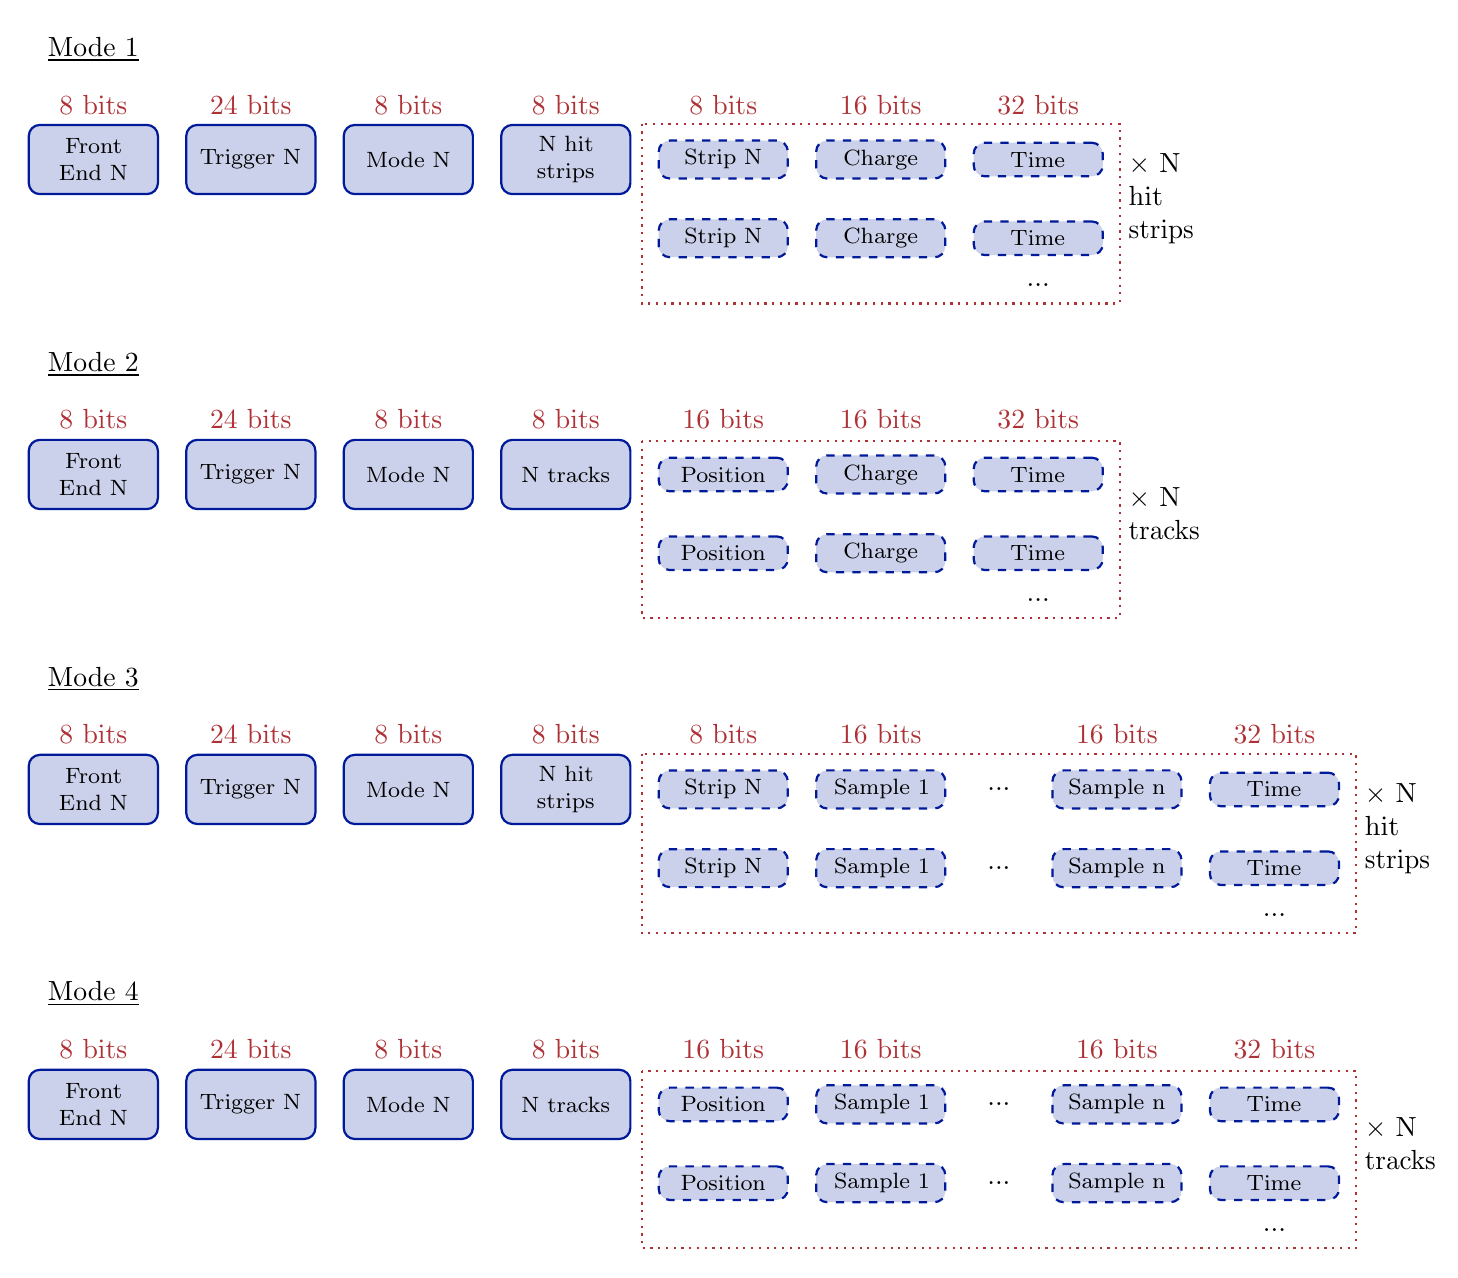
\begin{tikzpicture}
[%
    auto,
    block/.style={
      rectangle,
      draw=myColorMainA,
      thick,
      fill=myColorMainA!20,
      text width=4em,
      align=center,
      rounded corners,
      minimum height=2.5em,
      font=\footnotesize
    },
    block1/.style={
      rectangle,
      draw=myColorMainA,
      thick,
      dashed,
      fill=myColorMainA!20,
      text width=4em,
      align=center,
      rounded corners,
      minimum height=1em,
      font=\footnotesize
    },
    comment/.style={
    text width=2em,
    minimum height=7em
    }
  ]
  %Mode 1
  	\node at (0, -0.6) {\underline{Mode 1}};
  	\node at (0, -1.3) {\textcolor{myColorMainB}{8 bits}} ;
    \node at (2, -1.3) {\textcolor{myColorMainB}{24 bits}} ;
    \node at (4, -1.3) {\textcolor{myColorMainB}{8 bits}} ;
    \node at (6, -1.3) {\textcolor{myColorMainB}{8 bits}} ;
    \node at (8, -1.3) {\textcolor{myColorMainB}{8 bits}} ;
    \node at (10, -1.3) {\textcolor{myColorMainB}{16 bits}} ;
    \node at (12, -1.3) {\textcolor{myColorMainB}{32 bits}} ;
    \draw (0,-2) node[block] (FEN) {Front End N};
    \draw (2,-2) node[block] (TN) {Trigger N};
    \draw      (4,-2) node[block] (MN) {Mode N};
    \draw     (6,-2) node[block] (NHS) {N hit strips};
    \draw      (8,-2) node[block1] (SN) {Strip N};
    \draw     (10,-2) node[block1] (Q) {Charge};
    \draw     (12,-2) node[block1] (T) {Time};
    \draw      (8,-3) node[block1] (SN2) {Strip N};
    \draw     (10,-3) node[block1] (Q2) {Charge};
    \draw     (12,-3) node[block1] (T2) {Time};
    \node at (12,-3.6) {...};
	\draw     (13.5,-2.5) node[comment] (cm) {$\times$ N hit strips};
  
  	\draw[myColorMainB,thick,dotted] ($(SN.north west)+(-0.2,0.2)$)  rectangle ($(T2.south east)+(0.2,-0.6)$);
  	
  	%Mode 2
  	\node at (0, -4.6) {\underline{Mode 2}};
  	\node at (0, -5.3) {\textcolor{myColorMainB}{8 bits}} ;
    \node at (2, -5.3) {\textcolor{myColorMainB}{24 bits}} ;
    \node at (4, -5.3) {\textcolor{myColorMainB}{8 bits}} ;
    \node at (6, -5.3) {\textcolor{myColorMainB}{8 bits}} ;
    \node at (8, -5.3) {\textcolor{myColorMainB}{16 bits}} ;
    \node at (10, -5.3) {\textcolor{myColorMainB}{16 bits}} ;
    \node at (12, -5.3) {\textcolor{myColorMainB}{32 bits}} ;
    \draw (0,-6) node[block] (FEN) {Front End N};
    \draw (2,-6) node[block] (TN) {Trigger N};
    \draw      (4,-6) node[block] (MN) {Mode N};
    \draw     (6,-6) node[block] (NHS) {N tracks};
    \draw      (8,-6) node[block1] (SN) {Position};
    \draw     (10,-6) node[block1] (Q) {Charge};
    \draw     (12,-6) node[block1] (T) {Time};
    \draw      (8,-7) node[block1] (SN2) {Position};
    \draw     (10,-7) node[block1] (Q2) {Charge};
    \draw     (12,-7) node[block1] (T2) {Time};
    \node at (12,-7.6) {...};
	\draw     (13.5,-6.5) node[comment] (cm) {$\times$ N tracks};
  
  	\draw[myColorMainB,thick,dotted] ($(SN.north west)+(-0.2,0.2)$)  rectangle ($(T2.south east)+(0.2,-0.6)$);
  	
  	%Mode 3
  	\node at (0, -8.6) {\underline{Mode 3}};
  	\node at (0, -9.3) {\textcolor{myColorMainB}{8 bits}} ;
    \node at (2, -9.3) {\textcolor{myColorMainB}{24 bits}} ;
    \node at (4, -9.3) {\textcolor{myColorMainB}{8 bits}} ;
    \node at (6, -9.3) {\textcolor{myColorMainB}{8 bits}} ;
    \node at (8, -9.3) {\textcolor{myColorMainB}{8 bits}} ;
    \node at (10, -9.3) {\textcolor{myColorMainB}{16 bits}} ;
    \node at (13, -9.3) {\textcolor{myColorMainB}{16 bits}} ;
    \node at (15, -9.3) {\textcolor{myColorMainB}{32 bits}} ;
    \draw (0,-10) node[block] (FEN) {Front End N};
    \draw (2,-10) node[block] (TN) {Trigger N};
    \draw      (4,-10) node[block] (MN) {Mode N};
    \draw     (6,-10) node[block] (NHS) {N hit strips};
    \draw      (8,-10) node[block1] (SN) {Strip N};
    \draw      (10,-10) node[block1] (S1) {Sample 1};
    \node at (11.5, -10) {...};
    \draw     (13,-10) node[block1] (Sn) {Sample n};
    \draw     (15,-10) node[block1] (T) {Time};
    \draw      (8,-11) node[block1] (SN2) {Strip N};
    \draw      (10,-11) node[block1] (S12) {Sample 1};
    \node at (11.5, -11) {...};
    \draw     (13,-11) node[block1] (Sn2) {Sample n};
    \draw     (15,-11) node[block1] (T2) {Time};
    \node at (15,-11.6) {...};
	\draw     (16.5,-10.5) node[comment] (cm) {$\times$ N hit strips};
  
  	\draw[myColorMainB,thick,dotted] ($(SN.north west)+(-0.2,0.2)$)  rectangle ($(T2.south east)+(0.2,-0.6)$);
  	
  	%Mode 4
  	\node at (0, -12.6) {\underline{Mode 4}};
  	\node at (0, -13.3) {\textcolor{myColorMainB}{8 bits}} ;
    \node at (2, -13.3) {\textcolor{myColorMainB}{24 bits}} ;
    \node at (4, -13.3) {\textcolor{myColorMainB}{8 bits}} ;
    \node at (6, -13.3) {\textcolor{myColorMainB}{8 bits}} ;
    \node at (8, -13.3) {\textcolor{myColorMainB}{16 bits}} ;
    \node at (10, -13.3) {\textcolor{myColorMainB}{16 bits}} ;
    \node at (13, -13.3) {\textcolor{myColorMainB}{16 bits}} ;
    \node at (15, -13.3) {\textcolor{myColorMainB}{32 bits}} ;
    \draw (0,-14) node[block] (FEN) {Front End N};
    \draw (2,-14) node[block] (TN) {Trigger N};
    \draw      (4,-14) node[block] (MN) {Mode N};
    \draw     (6,-14) node[block] (NHS) {N tracks};
    \draw      (8,-14) node[block1] (SN) {Position};
    \draw      (10,-14) node[block1] (S1) {Sample 1};
    \node at (11.5, -14) {...};
    \draw     (13,-14) node[block1] (Sn) {Sample n};
    \draw     (15,-14) node[block1] (T) {Time};
    \draw      (8,-15) node[block1] (Sn2) {Position};
    \draw      (10,-15) node[block1] (S12) {Sample 1};
    \node at (11.5, -15) {...};
    \draw     (13,-15) node[block1] (Sn2) {Sample n};
    \draw     (15,-15) node[block1] (T2) {Time};
    \node at (15,-15.6) {...};
	\draw     (16.5,-14.5) node[comment] (cm) {$\times$ N tracks};
  
  	\draw[myColorMainB,thick,dotted] ($(SN.north west)+(-0.2,0.2)$)  rectangle ($(T2.south east)+(0.2,-0.6)$);
\end{tikzpicture}
\caption{Scatterer detector data format.}
\label{chapappA::fig::scattDataForm}
\end{figure}

\subsection{Absorber detector data format}\label{chapappA::subsec::absDataFormat}
The \gls{bgo} block readout is performed via the \gls{asm} cards. Each card is equipped with 24 input ports (signal \gls{pm}), corresponding to 6 \gls{bgo} blocks. Two possible working modes have been defined for the \gls{bgo} absorber: the collected total charge and time are evaluated on the card, or the \gls{pm} raw signals are sampled and the sampling is sent to the acquisition (\figurename~\ref{chapappA::fig::absDataForm}). Charge and time are then calculated at the analysis stage. This second operating mode can be useful in the test phase but it determines a low acquisition rate, so that it can be used only at low beam intensity.\newline
The complete sampling is stored in a dedicated buffer.

\begin{figure}[htbp]
\centering
\hspace*{-4em}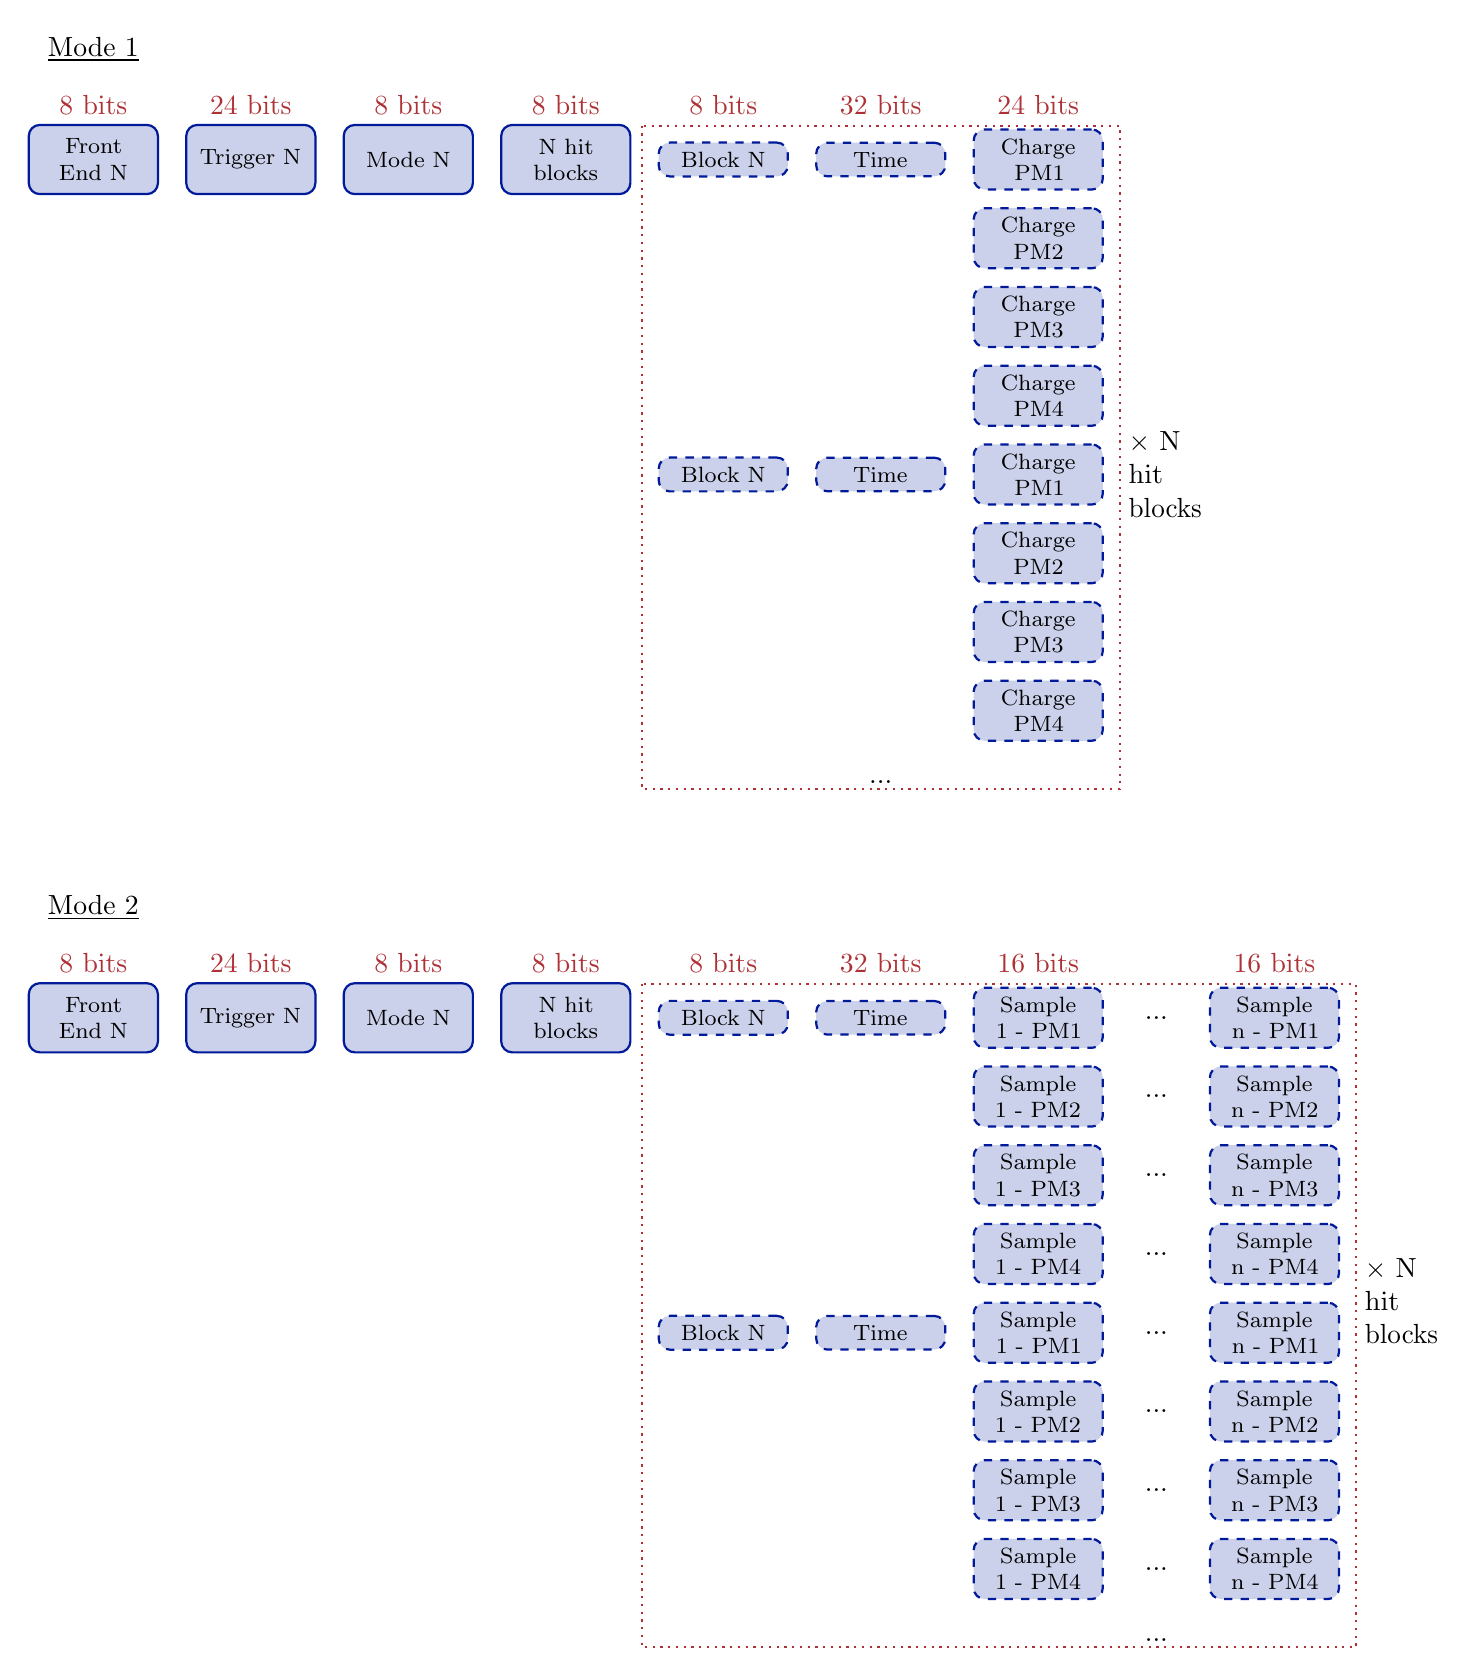
\begin{tikzpicture}
[%
    auto,
    block/.style={
      rectangle,
      draw=myColorMainA,
      thick,
      fill=myColorMainA!20,
      text width=4em,
      align=center,
      rounded corners,
      minimum height=2.5em,
      font=\footnotesize
    },
    block1/.style={
      rectangle,
      draw=myColorMainA,
      thick,
      dashed,
      fill=myColorMainA!20,
      text width=4em,
      align=center,
      rounded corners,
      minimum height=1em,
      font=\footnotesize
    },
    comment/.style={
    text width=2em,
    minimum height=7em
    }
  ]
  %Mode 1
  	\node at (0, -0.6) {\underline{Mode 1}};
  	\node at (0, -1.3) {\textcolor{myColorMainB}{8 bits}} ;
    \node at (2, -1.3) {\textcolor{myColorMainB}{24 bits}} ;
    \node at (4, -1.3) {\textcolor{myColorMainB}{8 bits}} ;
    \node at (6, -1.3) {\textcolor{myColorMainB}{8 bits}} ;
    \node at (8, -1.3) {\textcolor{myColorMainB}{8 bits}} ;
    \node at (10, -1.3) {\textcolor{myColorMainB}{32 bits}} ;
    \node at (12, -1.3) {\textcolor{myColorMainB}{24 bits}} ;
    \draw (0,-2) node[block] (FEN) {Front End N};
    \draw (2,-2) node[block] (TN) {Trigger N};
    \draw      (4,-2) node[block] (MN) {Mode N};
    \draw     (6,-2) node[block] (NHS) {N hit blocks};
    \draw      (8,-2) node[block1] (SN) {Block N};
    \draw     (10,-2) node[block1] (T) {Time};
    \draw     (12,-2) node[block1] (Q1) {Charge PM1};
    \draw     (12,-3) node[block1] (Q2) {Charge PM2};
	\draw     (12,-4) node[block1] (Q3) {Charge PM3};
    \draw     (12,-5) node[block1] (Q4) {Charge PM4};
    \draw      (8,-6) node[block1] (SN_2) {Block N};
    \draw     (10,-6) node[block1] (T_2) {Time};
    \draw     (12,-6) node[block1] (Q1_2) {Charge PM1};
    \draw     (12,-7) node[block1] (Q2_2) {Charge PM2};
	\draw     (12,-8) node[block1] (Q3_2) {Charge PM3};
    \draw     (12,-9) node[block1] (Q4_2) {Charge PM4};        
    \node at (10,-9.9) {...};
	\draw     (13.5,-6) node[comment] (cm) {$\times$ N hit blocks};
  
  	\draw[myColorMainB,thick,dotted] ($(SN.north west)+(-0.2,0.2)$)  rectangle ($(Q4_2.south east)+(0.2,-0.6)$);
  	
  	%Mode 2
  	\node at (0, -11.5) {\underline{Mode 2}};
  	\node at (0, -12.2) {\textcolor{myColorMainB}{8 bits}} ;
    \node at (2, -12.2) {\textcolor{myColorMainB}{24 bits}} ;
    \node at (4, -12.2) {\textcolor{myColorMainB}{8 bits}} ;
    \node at (6, -12.2) {\textcolor{myColorMainB}{8 bits}} ;
    \node at (8, -12.2) {\textcolor{myColorMainB}{8 bits}} ;
    \node at (10, -12.2) {\textcolor{myColorMainB}{32 bits}} ;
    \node at (12, -12.2) {\textcolor{myColorMainB}{16 bits}} ;
    \node at (15, -12.2) {\textcolor{myColorMainB}{16 bits}} ;
        
    \draw (0,-12.9) node[block] (FEN) {Front End N};
    \draw (2,-12.9) node[block] (TN) {Trigger N};
    \draw      (4,-12.9) node[block] (MN) {Mode N};
    \draw     (6,-12.9) node[block] (NHS) {N hit blocks};
    \draw      (8,-12.9) node[block1] (BN) {Block N};
    \draw     (10,-12.9) node[block1] (T) {Time};
    \draw     (12,-12.9) node[block1] (Q1) {Sample 1 - PM1};
    \node at (13.5,-12.9) {...};
	\draw     (15,-12.9) node[block1] (Qn) {Sample n - PM1};
	\draw     (12,-13.9) node[block1] (Q1_2) {Sample 1 - PM2};
    \node at (13.5,-13.9) {...};
	\draw     (15,-13.9) node[block1] (Qn_2) {Sample n - PM2};
	\draw     (12,-14.9) node[block1] (Q1_3) {Sample 1 - PM3};
    \node at (13.5,-14.9) {...};
	\draw     (15,-14.9) node[block1] (Qn_3) {Sample n - PM3};
	\draw     (12,-15.9) node[block1] (Q1_4) {Sample 1 - PM4};
    \node at (13.5,-15.9) {...};
	\draw     (15,-15.9) node[block1] (Qn_4) {Sample n - PM4};
	
	\draw      (8,-16.9) node[block1] (BN_2) {Block N};
    \draw     (10,-16.9) node[block1] (T_2) {Time};
    \draw     (12,-16.9) node[block1] (Q1_2) {Sample 1 - PM1};
    \node at (13.5,-16.9) {...};
	\draw     (15,-16.9) node[block1] (Qn_2) {Sample n - PM1};
	\draw     (12,-17.9) node[block1] (Q1_2_2) {Sample 1 - PM2};
    \node at (13.5,-17.9) {...};
	\draw     (15,-17.9) node[block1] (Qn_2_2) {Sample n - PM2};
	\draw     (12,-18.9) node[block1] (Q1_3_2) {Sample 1 - PM3};
    \node at (13.5,-18.9) {...};
	\draw     (15,-18.9) node[block1] (Qn_3_2) {Sample n - PM3};
	\draw     (12,-19.9) node[block1] (Q1_4_2) {Sample 1 - PM4};
    \node at (13.5,-19.9) {...};
	\draw     (15,-19.9) node[block1] (Qn_4_2) {Sample n - PM4};   
    \node at (13.5,-20.8) {...};
	\draw     (16.5,-16.5) node[comment] (cm) {$\times$ N hit blocks};
  
  	\draw[myColorMainB,thick,dotted] ($(BN.north west)+(-0.2,0.2)$)  rectangle ($(Qn_4_2.south east)+(0.2,-0.6)$);
  	
\end{tikzpicture}
\caption{Absorber detector data format.}
\label{chapappA::fig::absDataForm}
\end{figure}

\subsection{Beam hodoscope data format}\label{chapappA::subsec::hodoDataFormat}
The beam tagging hodoscope is composed of two perpendicular planes of 128 scintillating fibers each. Each fiber is read-out on the two sides, for a total of  512 read-out channels. The output signals are send via optical fibers to 8 64-channel \glspl{pm} H8500 by Hamamatsu. 8 \gls{fe} cards have been developed for the signal collection, one per \gls{pm}, and are equipped with two custom \glspl{asic} (32 channels each) and one \gls{fpga}.\newline
Concerning the \enquote{optimal} mode (1$^{\mathrm{st}}$ operating mode for the hodoscope), the only collected information are the ID of the involved fibers and the interaction time. The \glspl{asic} allow for a minimum time resolution of 10 ns; this means that if two particles interacts in the hodoscope within a 10 ns window, they will be considered as part of a single event.\newline
In test mode, the total collected charge can be calculated. This feature is useful to evaluate the detector aging effect due to radiation exposure. The charge measurement is anyway limited to a single channel per \gls{asic}, so to two channels per \gls{pm}. The \gls{asic} channel able to measure the charge is identified as "N$^{\circ}$ Fiber charge 1" and "N$^{\circ}$ Fiber charge 2".

\begin{figure}[htbp]
\centering
\hspace*{-4em}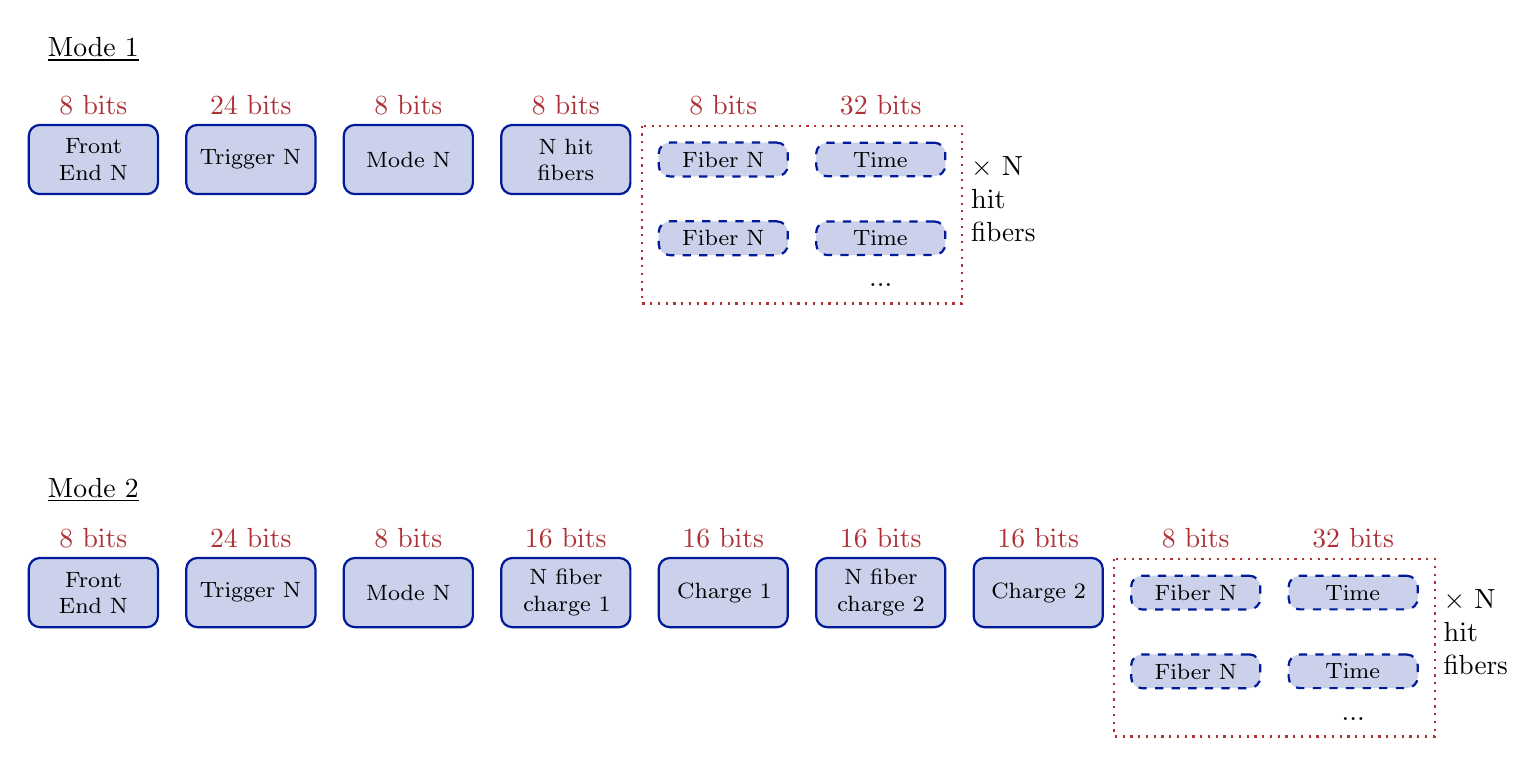
\begin{tikzpicture}
[%
    auto,
    block/.style={
      rectangle,
      draw=myColorMainA,
      thick,
      fill=myColorMainA!20,
      text width=4em,
      align=center,
      rounded corners,
      minimum height=2.5em,
      font=\footnotesize
    },
    block1/.style={
      rectangle,
      draw=myColorMainA,
      thick,
      dashed,
      fill=myColorMainA!20,
      text width=4em,
      align=center,
      rounded corners,
      minimum height=1em,
      font=\footnotesize
    },
    comment/.style={
    text width=2em,
    minimum height=7em
    }
  ]
  %Mode 1
  	\node at (0, -0.6) {\underline{Mode 1}};
  	\node at (0, -1.3) {\textcolor{myColorMainB}{8 bits}} ;
    \node at (2, -1.3) {\textcolor{myColorMainB}{24 bits}} ;
    \node at (4, -1.3) {\textcolor{myColorMainB}{8 bits}} ;
    \node at (6, -1.3) {\textcolor{myColorMainB}{8 bits}} ;
    \node at (8, -1.3) {\textcolor{myColorMainB}{8 bits}} ;
    \node at (10, -1.3) {\textcolor{myColorMainB}{32 bits}} ;
    \draw (0,-2) node[block] (FEN) {Front End N};
    \draw (2,-2) node[block] (TN) {Trigger N};
    \draw      (4,-2) node[block] (MN) {Mode N};
    \draw     (6,-2) node[block] (NHF) {N hit fibers};
    \draw      (8,-2) node[block1] (SN) {Fiber N};
    \draw     (10,-2) node[block1] (T) {Time};
    \draw      (8,-3) node[block1] (SN_2) {Fiber N};
    \draw     (10,-3) node[block1] (T_2) {Time};   
    \node at (10,-3.6) {...};
	\draw     (11.5,-2.5) node[comment] (cm) {$\times$ N hit fibers};
  
  	\draw[myColorMainB,thick,dotted] ($(SN.north west)+(-0.2,0.2)$)  rectangle ($(T_2.south east)+(0.2,-0.6)$);
  	
  	%Mode 2
  	\node at (0, -6.2) {\underline{Mode 2}};
  	\node at (0, -6.8) {\textcolor{myColorMainB}{8 bits}} ;
    \node at (2, -6.8) {\textcolor{myColorMainB}{24 bits}} ;
    \node at (4, -6.8) {\textcolor{myColorMainB}{8 bits}} ;
    \node at (6, -6.8) {\textcolor{myColorMainB}{16 bits}} ;
    \node at (8, -6.8) {\textcolor{myColorMainB}{16 bits}} ;
    \node at (10, -6.8) {\textcolor{myColorMainB}{16 bits}} ;
    \node at (12, -6.8) {\textcolor{myColorMainB}{16 bits}} ;
    \node at (14, -6.8) {\textcolor{myColorMainB}{8 bits}} ;
    \node at (16, -6.8) {\textcolor{myColorMainB}{32 bits}} ;
        
    \draw (0,-7.5) node[block] (FEN) {Front End N};
    \draw (2,-7.5) node[block] (TN) {Trigger N};
    \draw      (4,-7.5) node[block] (MN) {Mode N};
    \draw     (6,-7.5) node[block] (NHS) {N fiber charge 1};
    \draw      (8,-7.5) node[block] (BN) {Charge 1};
    \draw     (10,-7.5) node[block] (NHS) {N fiber charge 2};
    \draw      (12,-7.5) node[block] (BN) {Charge 2};
    \draw      (14,-7.5) node[block1] (SN) {Fiber N};
    \draw     (16,-7.5) node[block1] (T) {Time};
    \draw      (14,-8.5) node[block1] (SN_2) {Fiber N};
    \draw     (16,-8.5) node[block1] (T_2) {Time};  
     \node at (16,-9.1) {...};
	\draw     (17.5,-8) node[comment] (cm) {$\times$ N hit fibers}; 
    
  	\draw[myColorMainB,thick,dotted] ($(SN.north west)+(-0.2,0.2)$)  rectangle ($(T_2.south east)+(0.2,-0.6)$);
  	
\end{tikzpicture}
\caption{Beam hodoscope data format.}
\label{chapappA::fig::hodoDataForm}
\end{figure}

%%%%%%%%%%%%%%%%%%%%%%%%%%%%%%%%%%%%%%%%%%%%%%%%%%%%%%%%%%%%%%%%%%%%%%%%
%%%%%%%%%%%%%%%%%%%%%%%%%%%%%%%%%%%%%%%%%%%%%%%%%%%%%%%%%%%%%%%%%%%%%%%%
%%%%%%%%%%%%%%%%%%%%%%%%%%%%%%%%%%%%%%%%%%%%%%%%%%%%%%%%%%%%%%%%%%%%%%%%

\section{Slow control, trigger and monitoring data format}\label{chapappA::sec::slowCTrigMonDataFormat}

\subsection{Communication architecture}\label{chapappA::subsec::commArch}

The Endpoint architecture is composed of three layers:
\begin{itemize}
	\item application layer
	\item mac (or transport) layer/processor packet
	\item physical layer
\end{itemize}

	\begin{figure} [!hbtp]
	\centering
	\caption{Architecture of communication between DAQ cards and \gls{utca}.}
	\label{chapappA::fig::commDAQuTCA}
	\includegraphics[width=1\textwidth]{03_GraphicFiles/appendixA_dataFormat/DAQ_uTCAImage.pdf}
	\end{figure}


\subsection{Transport protocol and processor packets}\label{chapappA::subsec::transport}

\subsubsection{Definitions}\label{chapappA::subsubsec::transpDefs}
	It is worth to define some useful terms for the following part of the document:

	\begin{itemize}
		\item byte : 8 bits
		\item word : 16 bits
		\item K : control byte
		\item D : data byte
		\item cargo : data group
		\item terminator : packet end
		\item CRC : cyclic redundancy code \newline
	\end{itemize}

The CRC allows one to detect the transmission errors and the data transfer issues. A specific algorithm must be used, as CRC-16 : X16 + X15 + X2 + 1. In the present protocol, a \enquote{parity patter of 16 bits} have been used.

The transport layer ensures a proper packets exchange between two terminals via the data encapsulation. The data come from the application layer and are then sent to the physical layer.\newline
%\textbf{L'encapsulation choisie est 8 bits/10 bits.}\newline

\subsubsection{Data encoding}\label{chapappA::subsubsec::transpDataDec}
For the transport layer, the data structure is created via the addition of a packet header, corresponding to a parity bit, of a 16 bit parity pattern and a bit for the end of the packet.
The data are 8 bits/10 bits encoded. This standard 8 bits/10 bits encoding ensures sufficient data transitions for clock recovery.

\subsubsection{Packets format}\label{chapappA::subsubsec::transpPackForm}

All the data packets have the same structure. A K byte (control symbol) is followed by the cargo to be sent. The end of the packets changes according to the cargo parity.\newline
If the cargo contains an even number of bytes, the packet ends with K.28.6.

\begin{table} [!htbp]
\centering
\caption{Packet with an even byte number cargo.}
\label{chapappA::tab::EvenCargo}
\begin{tabular}{m{1.5cm} M{2.5cm} M{2.5cm} M{4cm}}
\toprule
\rowcolor{myColorMainA!20}
\textbf{Item}  	&\textbf{Packet beginning}		&\textbf{Cargo} 	&\textbf{Packet end}\\
\midrule
1				& One K byte 					& 0 - N D-bytes		& K.28.6	\\
\bottomrule
\end{tabular}
\end{table}

If the cargo contains an odd number of bytes, the packet ends without any control symbol.

\begin{table} [!htbp]
\centering
\caption{Packet with an odd byte number cargo.}
\label{chapappA::tab::OddCargo}
\begin{tabular}{m{1.5cm} M{2.5cm} M{2.5cm} M{4cm}}
\toprule
\rowcolor{myColorMainA!20}
\textbf{Item}  	&\textbf{Packet beginning}		&\textbf{Cargo} 	&\textbf{Packet end}\\
\midrule
1				& One K byte						& 0 - N D-bytes		& Beginning of a new packet	\\
\bottomrule
\end{tabular}
\end{table}

\underline{Remark} :
	\begin{itemize}
		\item SYN packet is a special kind of packet starting with K.28.6 and ending with K.28.5. It is only composed of these two bytes (16 bits). It allows the receiver to find the beginning and the end of the transmitted bytes with the aim to reconstruct the events in parallel. The synchronization speed is 44 Hz (defined by Carlos Abellan).
		\item In order to optimize the throughput, the control symbol at the beginning of the packet can probably be removed (further study needed).
		\end{itemize}



\subsubsection{Possible control symbols}\label{chapappA::subsubsec::ctrlSymbols}

In \tablename~\ref{chapappA::tab::ControlSymbol}, all the possible control symbols are listed (defined by Carlos Abellan).

\begin{table} [!htbp]
\centering
\caption{Control symbol definition.}
\label{chapappA::tab::ControlSymbol}
\begin{tabular}{m{1.5cm} M{2.5cm} M{2.5cm} M{4cm}}
\toprule
\rowcolor{myColorMainA!20}
\textbf{Item}  			&\textbf{Name}		&\textbf{Control code}	&\textbf{Comment}\\
\midrule
1						&K.28.0				&	0x1C					&	Acknowledgement\\
2						&K.28.1				&	0x3C					&	Ask for writing registers\\
3						&K.28.2				&	0x5C					&	Ask for reading registers\\
4						&K.28.3				&	0x7C					&	Special command\\
5						&K.28.4				&	0x9C					&	Monitoring\\
6						&K.28.5				&	0xBC					& 	Default synchronization\\
7						&K.28.6				&	0xDC					& 	IDLE (default) and packet end\\
8						&K.28.7				&	0xFC					&	Pre-trigger\\
9						&K.23.7				&	0xF7					&	Trigger \\
10						&K.27.7				&	0xFB					&	\\
11						&K.29.7				&	0xFD					&	\\
12						&K.30.7				&	0xFE					&	Physical data\\
\bottomrule
\end{tabular}
\end{table}


\subsection{Transport layer}\label{chapappA::subsec::transpLayer}

\subsubsection{Control packet}\label{chapappA::subsubsec::ctrlPacket}

This kind of packet is used to check the link and for the control/command operations.
\begin{itemize}
\item For the link check, two kinds of packets are used: synchronization packet and IDLE packet.
\item For the control/command operations, here are some examples: register configuration,  \gls{fpga} dynamical programming, monitoring, etc.\newline
\end{itemize}

\underline{Control symbol for control} :

\begin{table} [!htbp]
\centering
\caption{Control symbol definition.}
\label{chapappA::tab::ControlSymbolDef}
\begin{tabular}{m{1.5cm} M{2.5cm} M{2.5cm} M{4cm}}
\toprule
\rowcolor{myColorMainA!20}
\textbf{Item}  			& 		\textbf{Name}		& \textbf{Control code}	& \textbf{Comment}\\
\midrule
1				&	K.28.0			&	0x1C			& Acknowledgement	\\
2				&	K.28.1			&	0x3C			& Ask for writing registers	\\
3				&	K.28.2			&	0x5C			& Ask for reading registers	\\
4				&	K.28.3			&	0x7C			& Special command	\\
5				&	K.28.4			&	0x9C			& Monitoring	\\
6				&	K.28.5			&	0xBC		& Synchronization	\\
7				&	K.28.6			&	0xDC		& IDLE (default) and end of packet\\
\bottomrule
\end{tabular}
\end{table}


\underline{Acknowledgement packet (Front End cards $\rightarrow$ \gls{utca})}\newline

This packet is sent by the \gls{fe} cards and interpreted as an acknowledgement by the \gls{utca}. If a part is missing, it is set to zero.
\begin{itemize}
	\item If 0 = validation
	\item If 1 = problem detected
\end{itemize}


\begin{table} [!htbp]
\centering
\caption{Definition of the acknowledgement packet.}
\label{chapappA::tab::AcknPacket}
\begin{tabular}{p{1cm} P{2cm} P{1cm}P{1cm}P{1cm}P{1cm}P{1cm}P{1cm}P{1cm}P{1cm}}
\toprule
\rowcolor{myColorMainA!20}
\textbf{Word}  			& 		\textbf{1$\mathrm{^{st}}$ byte}		& \multicolumn{8}{c}{\textbf{2$\mathrm{^{nd}}$ byte}} 	\\
\midrule
					&						& 7b & 6b& 5b&4b&3b&2b&1b&0b \\
					\cmidrule{3-10}
1				&	K.28.0			&	0	& Pb Front End number & Pb with packet beginning & Pb with packet end & Pb with CRC & Pb with number of received words &  Pb with parity bit of byte 2 & parity bit of the acknowledgement packet	\\
\midrule
2				& \multicolumn{9}{c}{Front End number}\\
\bottomrule
\end{tabular}
\end{table}

\subsubsection{Configuration packets}\label{chapappA::subsubsec::confPackets}

\underline{Writing register process (\gls{utca} $\rightarrow$ Front End cards)}\newline

The process starts with a packet sent by the \gls{utca} asking for the register writing. The receiver (\gls{fe} card) sends back an acknowledgement packet to finish the process. In \tablename~\ref{chapappA::tab::WriteRegister} the format of this writing register packet is reported.

\begin{table} [!htbp]
\centering
\caption{Writing register packet.}
\label{chapappA::tab::WriteRegister}
\begin{tabular}{m{1.5cm} M{2cm} M{3cm} M{5.5cm}}
\toprule
\rowcolor{myColorMainA!20}
\textbf{Word}  			& 	\textbf{1$\mathrm{^{st}}$ byte}	& \textbf{2$\mathrm{^{nd}}$ byte} & \textbf{Comment} \\
\midrule
1				&	K.28.1	& Front End number + 1 parity bit		& N/A  \\
\cmidrule{2-4}
2				&\multicolumn{2}{M{5cm}}{2 bytes with the number of words to be written}& The length is word-based: max $2^{16}-~1$~=~65535 words\\
\cmidrule{2-4}
3 			&      \multicolumn{2}{M{5cm}}{Register address} 		& Address where the writing process starts\\
\cmidrule{2-4}
4..N+3        	&      \multicolumn{2}{M{5cm}}{Data to be written} 		&0000 0000\\
\cmidrule{2-4}
N+4				 & \multicolumn{2}{M{5cm}}{CRC composed of the \enquote{xor} of all bits in the same position, from word 2 to word (N+3)} 		& 	\\
\bottomrule
\end{tabular}
\end{table}


\underline{Reading register process (\gls{utca} $\rightarrow$ Front End cards)}\newline

The process starts with a packet sent by the \gls{utca} asking for the register reading. The receiver (\gls{fe} card) sends back the \enquote{measure packet} if the command is correct, an acknowledgement packet if it is not.\newline
At the beginning of the slow control, the physical addresses on the \gls{fe} cards are read at the address 0.\newline
In \tablename~\ref{chapappA::tab::readRegPacket} the format of this reading register packet is reported.

\begin{table} [!htbp]
\centering
\caption{Reading register packet.}
\label{chapappA::tab::readRegPacket}
\begin{tabular}{m{1.5cm} M{2cm} M{3cm} M{5.5cm}}
\toprule
\rowcolor{myColorMainA!20}
\textbf{Word}  			& 	\textbf{1$\mathrm{^{st}}$ byte}	& \textbf{2$\mathrm{^{nd}}$ byte} & \textbf{Comment} \\
\midrule
1				&	K.28.2	& Front End number + 1 parity bit &  N/A \\
\cmidrule{2-4}
2				&\multicolumn{2}{M{5cm}}{2 bytes with the number of words to be read}	& The length is word-based: max $2^{16}-~1$~=~65535 words\\
\cmidrule{2-4}
3 			&      \multicolumn{2}{M{5cm}}{Address of 1$\mathrm{^{st}}$ data to be read} & Address where the reading process starts\\
\cmidrule{2-4}
4				 & \multicolumn{2}{M{5cm}}{CRC composed of the \enquote{xor} of all bits in the same position, from word 2 to word 3} & /\\
\bottomrule
\end{tabular}
\end{table}

\begin{table} [!htbp]
\centering
\caption{Two special registers(\gls{utca} $\rightarrow$  Front End cards)}
\label{chapaapA::tab::twoSpecReg}
\begin{tabular}{m{1.5cm} M{5.25cm} M{5.25cm} }
\toprule
\rowcolor{myColorMainA!20}
\textbf{Register address}  			& 	\textbf{Details}	& \textbf{Comment} \\
\midrule
0				&	Front End number		&  No writing rights: register in read-only mode. Hard coded on DAQ card.\\
\cmidrule{2-3}
1				&    It defines the working modes & Optimal mode, test mode, collimated camera mode, Compton camera mode, individual detector section test. It is possible to write in the register.  \\
\cmidrule{2-3}
2				& It defines the detector to test (in single detector test mode)		& Scatterer, absorber, hodoscope.\\
\cmidrule{2-3}
3 				& \gls{bgo} number of sampling		& For test mode with the \gls{bgo} blocks signal sampling.\\
\cmidrule{2-3}
4				& Silicon number of sampling	& For test mode with the silicon layers signal sampling.\\
\bottomrule
\end{tabular}
\end{table}


\begin{table} [!htbp]
\centering
\caption{Measurement packet (Front End cards $\rightarrow$ \gls{utca})}
\label{chapappA::tab::measPacket}
\begin{tabular}{m{1.5cm} M{2cm} M{3cm} M{5.5cm}}
\toprule
\rowcolor{myColorMainA!20}
\textbf{Word}  			& 	\textbf{1$\mathrm{^{st}}$ byte}	& \textbf{2$\mathrm{^{nd}}$ byte} & \bf{Comment} \\
\midrule
1				&	K.28.1	&Front End number + 1 parity bit		&\\
\cmidrule{2-4}
2				&\multicolumn{2}{M{5cm}}{2 bytes for the number of data words to send}& The length is word-based: max $2^{16}-~1$~=~65535 words\\
\cmidrule{2-4}
3 			&      \multicolumn{2}{M{5cm}}{Register address} & Address where the writing process starts\\
\cmidrule{2-4}
4..N+3        	&      \multicolumn{2}{M{5cm}}{Read data} &0000 0000\\
\cmidrule{2-4}
N+4				 & \multicolumn{2}{M{5cm}}{CRC composed of the \enquote{xor} of all bits in the same position, from word 2 to word (N+3)}&/\\
\bottomrule
\end{tabular}
\end{table}


\subsubsection{Monitoring process (Front End cards $\rightarrow$ \gls{utca})}\label{chapappA::subsubsec::monitorProcess}

In case of issues, for example when the temperature of a card go beyond a fixed threshold, the DAQ card sends a \enquote{monitoring} packet to the \gls{utca}. There is not a corresponding acknowledgement from the \gls{utca}.\newline


\begin{table} [!htbp]
\centering
\caption{Monitoring packet.}
\label{chapappA::tab::monitorPacket}
\begin{tabular}{m{1.5cm} M{2cm} M{3cm} M{5.5cm}}
\toprule
\rowcolor{myColorMainA!20}
\textbf{Word}  			& 	\textbf{1$\mathrm{^{st}}$ byte}	& \textbf{2$\mathrm{^{nd}}$ byte} & \textbf{Comment} \\
\midrule
	1				&	K.28.4.		& Front End number + 1 parity bit & Message in \tablename~\ref{chapappA::tab::monitoringMess}.\\
\cmidrule{2-4}
	2				&	 \multicolumn{2}{M{5cm}}{15 bits for the message + 1 parity bit} 	& Message in \tablename~\ref{chapappA::tab::monitoringMess}.\\
\bottomrule
\end{tabular}
\end{table}

\begin{table} [!htbp]
\centering
\caption{Monitoring messages.}
\label{chapappA::tab::monitoringMess}
\begin{tabular}{m{0.6cm} M{1.3cm} M{1.cm} M{0.8cm} M{0.8cm} M{0.8cm} M{0.8cm} M{0.8cm} M{0.8cm} M{0.8cm} M{0.8cm} M{2.5cm}}
\toprule
\rowcolor{myColorMainA!20}
\textbf{Item}  			& 		\textbf{Message}		& \textbf{Bit[15] } & \textbf{...} &\textbf{Bit[7]} & \textbf{Bit[6]} & \textbf{Bit[5]} & \textbf{Bit[4]} & \textbf{Bit[3]} & \textbf{Bit[2]} & \textbf{Bit[1]} & \textbf{Comment}\\
\midrule
				&						& \multicolumn{6}{M{5.cm}}{Message type} & \multicolumn{3}{M{2.4cm}}{Further information} & \\
\cmidrule{3-11}
1				&	\gls{fpga} reconfiguration error 			&0&0&	0	& 0&0&1&0&0&0& N/A	\\
\cmidrule{3-11}
2				&	Tem\-pe\-ra\-tu\-re alarm 			&0&0&	0	& 0&1&0&x&x&x& Bit \enquote{x} is 1 if the corresponding detector goes beyond the threshold (0 elsewhere)\\
\cmidrule{3-11}
3				&	Busy							&0&0&	0	& 1&0&0&0&0&0&Front End is not able to send data\\
\cmidrule{3-11}
...				&								&	& &	& & & & & & & \\
\bottomrule
\end{tabular}
\end{table}


\subsubsection{Special command process (\gls{utca} $\rightarrow$ Front End cards)}\label{chapappA::subsec::specCmdProcess}

This process is designed to allow the \gls{utca} to send special commands to the \gls{fe} cards.

\begin{table} [!htbp]
\centering
\caption{Special command packets}
\label{chapappA::tab::specCmdPacket}
\begin{tabular}{m{1.5cm} M{5.25cm} M{5.25cm} }
\toprule
\rowcolor{myColorMainA!20}
\textbf{Word}  			& 	\textbf{1$\mathrm{^{st}}$ byte}	& \textbf{2$\mathrm{^{nd}}$ byte}\\
\midrule
1			& K.28.3	& Front End number + 1 parity bit\\

2				&	 \multicolumn{2}{M{10.5cm}}{15 bits for the special command + 1 parity bit}\\
\bottomrule
\end{tabular}
\end{table}

\begin{table} [!htbp]
\centering
\caption{Special commands examples}
\label{chapappA::tab::specCmdExamples}
\begin{tabular}{m{1.5cm} M{4cm} M{4cm} M{4cm}}
\toprule
\rowcolor{myColorMainA!20}
\textbf{Item}  			& 	\textbf{Command name}	& \textbf{Bit[15..1] of 2$\mathrm{^{nd}}$ word} & \textbf{Comment} \\
\midrule
	1				&	System reset				& "0000 0000 0001  001"  	& Acknowledgement packet missing \\
	2				&	Counter reset			& "0000 0000 0001  000"  	& Acknowledgement packet needed \\
	3				&	Start run					& "0000 0000 0000  100"  	& Acknowledgement packet needed\\
	4				&	Stop run					& "0000 0000 0000  101" 	& Acknowledgement packet needed\\
	5				&	Dynamical \gls{fpga} configuration		& "0000 0000 0000  010" 	& Acknowledgement packet needed\\
	6				&	Veto						& "0000 0000 0000  011" 	& Example: \gls{utca} cannot receive the data. Acknowledgement packet needed\\
\bottomrule
\end{tabular}
\end{table}

A register database (containing the operating mode identification) must be fixed and shared between all the detectors.

\subsection{Data packets (Front End card $\rightarrow$ \gls{utca})}\label{chapappA::subsec::dataPackets}

In the section the packets concerning trigger, pre-trigger and physical data are described.\newline
No acknowledgement is demanded for this kind of packets.

\begin{table} [!htbp]
\centering
\caption{Control symbol for pre-trigger, trigger and physical data.}
\label{chapappA::tab::ctrlSymbolTrigData}
\begin{tabular}{m{1.0cm} M{2cm} M{2cm} M{5cm}}
\toprule
\rowcolor{myColorMainA!20}
\textbf{Item}  			& 	\textbf{Name}	& \textbf{Control code} & \textbf{Comment} \\
\midrule
	1				&	K.28.7	& 0xFC  	& The pre-trigger is generated by the \gls{thor} card and sent to the \gls{utca} who shares it with the silicon layers cards. \\
	2				&	K.23.7	& 0xF7  	& The trigger is generated by a single silicon layer card and sent to the \gls{utca} who shares it with all the \gls{fe} cards.\\

	5				&	K.30.7	& 0xFE	& The \gls{fe} cards send the data.  \\
\bottomrule
\end{tabular}
\end{table}

\underline{Pre-trigger format\newline}

This packet is sent to the \gls{utca} by the \gls{thor} card. The \gls{utca} then shares it with all the silicon \gls{fe} cards.\newline

\begin{table} [!htbp]
\centering
\caption{Pre-trigger packet}
\label{chapappA::tab::preTrigPacket}
\begin{tabular}{m{1.cm} M{3cm} M{5cm}}
\toprule
\rowcolor{myColorMainA!20}
\textbf{Item}  			& 	\textbf{1$\mathrm{^{st}}$ byte}	& \textbf{2$\mathrm{^{nd}}$ - 4$\mathrm{^{th}}$ bytes}\\
\midrule
1			& K.28.7	&	24 bits for the trigger number\\
\bottomrule
\end{tabular}
\end{table}

\underline{Trigger format\newline}

This packet is sent back to the \gls{utca} if a silicon \gls{fe} card finds an interaction in coincidence after the reception of the pre-trigger packet. The trigger is always sent before the physical data packets. The  \gls{utca} then sends the trigger packet to all the \gls{fe} cards (scatterer, absorber, hodoscope).

\begin{table} [!htbp]
\centering
\caption{Trigger packet}
\label{chapappA::tab::triggerPacket}
\begin{tabular}{m{1.cm} M{3cm} M{5cm}}
\toprule
\rowcolor{myColorMainA!20}
\textbf{Item}  			& 	\textbf{1$\mathrm{^{st}}$ byte}	& \textbf{2$\mathrm{^{nd}}$ - 4$\mathrm{^{th}}$ bytes}\\
\midrule
1			& K.23.7	&	24 bits for the trigger number\\
\midrule
\end{tabular}
\end{table}

\underline{Physical data packet format\newline}

This packet sends the \enquote{useful} data to the \gls{utca}. The data format (cargo) is defined in chapter 3.

\begin{table} [!htbp]
\centering
\caption{Physical data packet}
\label{chapappA::tab::physDataPacket}
\begin{tabular}{m{1.cm} M{3cm} M{3cm} M{3cm}}
\toprule
\rowcolor{myColorMainA!20}
\textbf{Item}  			& 	\textbf{1$\mathrm{^{st}}$ byte}	& \textbf{Cargo} & \textbf{End of packet} \\
\midrule
	1				&	K.30.7.		& From 0 to Nbr-1 words of D characters & K.28.6 or the beginning of a new packet.\\
\bottomrule
\end{tabular}
\end{table}

\section{UDP packets format}\label{chapappA::sec::UDPpackForm}

Once the \gls{utca} receives the data from the \gls{fe} cards, a physical event is generated and stored in dedicated buffers. The buffers are then sent to the acquisition PC via UDP packets. Each detector section has its own UDP socket, and three receiving ports are used for the three data fluxes: 60001 for the hodoscope, 60002 for the absorber, 60003 for the scatterer. The content of the data buffers are sent in order to avoid to divide events in different packets, so that each UDP packet is completely independent from the others and contains complete events. The maximum size of a packet is set to 1500 (UDP data = 1472), or to 9000 for the so called \enquote{jumbo frames}, used for high speed acquisitions.\newline
Each UDP packet has a custom defined header, composed of:
\begin{itemize}
\item 32 bits: packet number, starting from 0;
\item 16 bits: number of data structures in the packet;
\end{itemize}
The data structures are then in a list one after the other with the already described format.

\section{Data throughput expected in clinical conditions}\label{chapappA::sec::dataThroughputClinic}

\subsection{Clinical intensities}\label{chapappA::subsec::clinIntensity}

In clinical standards, the beam maximum intensity is:
\begin{itemize}
	\item protons : $10^{10}$ protons/s
	\item carbon ions : $5\times10^7$ C ions/s\newline
\end {itemize}
 %\textbf{Suite à de diverses discussions, tout le monde valide ces chiffres.}\newline

The Compton camera must be designed in order to be able to handle the whole range of clinical intensities. The design reference is then the maximum intensity, about 3.2 nA ($2\times10^{10}$ protons/s) delivered by the cyclotron C230 by IBA. The number of proton delivered per second is higher then the maximum considered rate ($10^{10}$ protons/s).\newline
As shown by the simulation results, the Compton camera can not be used for an online monitoring at the maximum beam intensity for both proton and carbon ion beams. The main limitation comes from the amount of random coincidences detected by the camera for high intensity beams. One possible solution is to deliver a lower intensity beam for the range monitoring before the beginning of the treatment. The results shown here relates to a reduced intensity, corresponding to the one selected via the simulation studies.

\subsubsection{Review: detector and target sizes}\label{chapappA::subsubsec::revDetTargetSize}

Detectors sizes:
\begin{itemize}
	\item Silicon scatterer : 7 silicon layers, 9.6$\times$9.6$\times$0.2 cm$\mathrm{^{3}}$ (first layer 20 cm far from the beam line)
	\item \gls{bgo} absorber: \gls{bgo} block 3.5$\times$3.8$\times$3.0 cm$\mathrm{^{3}}$ (67.5 cm far from the beam line - center of the block)\newline
\end{itemize}
\gls{pmma} target size: cylindrical shape, diameter 15 cm,  20 cm length along the beam direction.


\subsection{Coincidence rate}\label{chapappA::subsec::coincRate}

In \tablename~\ref{chapappA::tab::coincSingleRate} the coincidence and single (pre-trigger) rates expected for the different detector section are listed according to the beam kind and intensity. This values correspond the Compton camera, while for the collimated camera a reduced rate is expected for the absorber due to the presence of the physical collimator.

\begin{table} [!htbp]
\centering
\caption{Coincidence and single rate as a function of the beam intensity. The \gls{bgo} single rate corresponds to the pre-trigger rate.}
\label{chapappA::tab::coincSingleRate}
\begin{tabular}{m{3.2cm} c c c c c c}
\toprule
\rowcolor{myColorMainA!20}
		& \multicolumn{2}{c}{\textbf{Clinical intensity}} &\multicolumn{2}{c}{\textbf{Reduced intensity}} &\multicolumn{2}{c}{ \textbf{Collimated camera}}\\
\midrule		
		& \underline{Protons}& \underline{Carbon ions} & \underline{Protons}& \underline{Carbon ions} &\underline{Protons}& \underline{Carbon ions} \\
\midrule
\textbf{Intensity(ions/s)}		& $2\times10^{10}$	&$5\times10^{7}$  & $1\times10^{8}$& $5\times10^{6}$ &$2\times10^{10}$& $5\times10^{7}$ \\
\textbf{Coincidence rate per incident ion}		& $9\times10^{-4}$&  $8\times10^{-4}$&  $9\times10^{-4}$& $8\times10^{-4}$& / &  / \\
\textbf{Coincidence rate (Hz)}		& $1,8\times10^{7}$&  $4\times10^{4}$&  9$\times10^{4}$& $4\times10^{3}$& / &  / \\
\textbf{Single rate \gls{bgo} (Hz) - 96 blocks}		& 	$7,8\times10^{7}$& $1,4\times10^{6}$ & $3,9\times10^{5}$&$1,4\times10^{5}$ &/&/\\
\textbf{Single rate \gls{bgo} (Hz) - 1 block}		& 	$8,1\times10^{5}$& $1,5\times10^{4}$ & $4\times10^{3}$&$1,5\times10^{3}$ &/&/\\
\textbf{Single rate \gls{bgo} (Hz) - 1 \gls{asm} card (6 blocks)}		& 	$6,5\times10^{6}$& $1,2\times10^{5}$ & $3,2\times10^{4}$&$1,2\times10^{4}$ &/&/\\
\bottomrule
\end{tabular}
\end{table}


The application of the Compton camera at clinical intensity seems not feasible. The caemra distance with respect to the beam line should be increased to lower the rate to 1$\mathrm{\times10^{5}}$ Hz (which means to put the 1$\mathrm{^{st}$ silicon layer 1 m far from the beam line).
For a carbon ion beam at $5\times10^{7}$ Hz, the estimated coincidence rate is $4\times10^{4}$ Hz, with $1,4\times10^{6}$ single rate on the absorber (measurements of coincidence rate on the HIT accelerator adapted to a real camera size with a 40 ns coincidence window, Krimmer ANIMMA 2013).
The data flow between the \gls{utca} and the acquisition PC corresponds to the coincidence rate, due to the fact that only coincidence events are stored.


\subsection{Data flow (Front End cards  $\rightarrow$ \gls{utca})\newline}\label{chapappA::subsec::dataFlow}

The data format previously described has been used to evaluate the data flow between each \gls{fe} card and the \gls{utca}. The calculation is performed according to the \enquote{optimal} mode of each detector. For the \gls{bgo}, we only consider events where the 4 \glspl{pm} are involved. For the silicon layers, two cases are considered:
\begin{itemize}
	\item Case 1 : one single layer with 6 involved strips;
	\item Case 2 : all the 7 layers involved with 6 hit strips per layer.
\end{itemize}
Concerning the hodoscope, we considered an event with one hit fiber readout on the two sides.\newline
The 8bits/10bits encoding in included in the calculation.

\begin{table} [!htbp]
\centering
\caption{Data flux between \gls{fe} cards and \gls{utca}.}
\label{chapappA::tab::dataFlowFEuTCA}
\begin{tabular}{m{3.5cm} c c c c}
\toprule
\rowcolor{myColorMainA!20}
		&\multicolumn{2}{c}{\textbf{Clinical intensity}} &\multicolumn{2}{c}{\textbf{Reduced intensity}} \\
\midrule
		& \underline{Protons}& \underline{Carbon ions} & \underline{Protons}& \underline{Carbon ions} \\
\midrule
\textbf{Intensity (ions/s)}		& $2\times10^{10}$	&$5\times10^{7}$  & $1\times10^{8}$& $5\times10^{6}$  \\
\textbf{Pre-trigger flux (Mbits/s)}		& 	$2,5\times10^{3}$& 47,6 &  13,3&4,76 \\
\textbf{Trigger flux (Mbits/s)}		& 	612& 1,4 & 3,1&0,1\\
\textbf{\gls{bgo} data flux (Mbits/s) - 96 blocks}		& 	$1,7\times10^{5}$& 373 & 873&37,3\\
\textbf{\gls{bgo} data flux (Mbits/s)- 1 block}		& 	$1,7\times10^{3}$& 3,88 & 8,73&0,3 \\
\textbf{\gls{bgo} data flux (Mbits/s) - 1 carte \gls{asm}}		& 	$1,4\times10^{4}$& 31,1 & 69,9&3,1\\
\textbf{Silicon data flux (Mbits/s) - case 1}		& 	$2,3\times10^{5}$& 522 & $1,2\times10^{3}$ & 52,2 \\
\textbf{Silicon data flux (Mbits/s) - case 2}		& 	$1,6\times10^{6}$&  $ 3,7\times10^{3}$ &  $8,2\times10^{3}$&366 \\
\textbf{Hodosocpe data flux (Mbits/s)}		& 	$8,1\times10^{4}$& 180 & 404 &18\\
\bottomrule
\end{tabular}
\end{table}



\subsection{Acquisition data flow (\gls{utca} $\rightarrow$ Acquisition PC)}\label{chapappA::subsec::daqDataFlow}

The data flow from the \gls{utca} to the acquisition PC is detailed here. The UDP encoding is included in the calculation.

\begin{table} [!htbp]
\centering
\caption{Data flow between \gls{utca} and acquisition PC.}
\label{chapappA::tab::dataFlowuTCAPC}
\begin{tabular}{m{3.5cm} c c c c}
\toprule
\rowcolor{myColorMainA!20}
		&\multicolumn{2}{c}{	\textbf{Clinical intensity}} &\multicolumn{2}{c}{ \textbf{Reduced intensity}} \\
\midrule
		& \underline{Protons}& \underline{Carbon ions} & \underline{Protons}& \underline{Carbon ions} \\
\midrule
\textbf{Intensity (ions/s)}		& $2\times10^{10}$	&$5\times10^{7}$  & $1\times10^{8}$& $5\times10^{6}$\\
\textbf{Coincidence rate per incident ion}		& $9\times10^{-4}$&  $8\times10^{-4}$&  $9\times10^{-4}$& $8\times10^{-4}$ \\
\textbf{Coincidence rate (Hz)}		& $1,8\times10^{7}$&  $4\times10^{4}$&  9$\times10^{4}$& $4\times10^{3}$\\
\textbf{Data flow (Mbits/s) - case 1}		&$2,2\times10^{4}$ &  46,7&  112& 5,0\\
\textbf{Data flow (Mbits/s) - case 2}		& $6\times10^{4}$&  133&  300& 13,3\\
\bottomrule
\end{tabular}
\end{table}

\subsection{Conclusions}\label{chapappA::subsec::conclusions}

As already mentioned, the Compton camera application is not feasible at clinical beam intensities. \newline
In order to have an online monitoring of the beam range, a reduced intensity must be foreseen. The main limitation is the rate of random coincidences detected at high intensity, while from the technological point of view no limitations are highlighted by this study. In the collimated camera configuration, where no coincidences are required and the random coincidences limitation is removed, we can then expect to be able to work at real clinical intensity.


% Appendix B
\input{02_Content/Appendix/AppendixB_Electronics.tex}

\endappendix

%%GLOSSARY and list of ACRONYMS
\cleardoublepage

%\printglossaries
\setglossarystyle{mystyle}
\printglossary[title=List of abbreviations, type=\acronymtype]


%%BIBLIOGRAPHY
\cleardoublepage
%\autocite{citekey} % Use
%\newrefsection
%\saverefsection
%\newrefcontext[sorting=nty]
%\nocite{\ReferencesList}

\printbibliography%Print bibliography

\printindex%Print analytical index

%Acknowledgements
\input{02_Content/Acknoledgements/Acknoledgements.tex}

\end{document}
% ------------------------------------------------------------------
%
% #######################
% End: Document
% #######################
